\documentclass[english, 12pt, a4paper, sci, utf8, a-2b, online]{aaltothesis}
\setupthesisfonts

\usepackage[linesnumbered, ruled, vlined]{algorithm2e}
\usepackage{todonotes}

\usepackage{svg}
\usepackage{subcaption}
\usepackage{minted}
\usepackage{float}
\usepackage{graphicx}
\usepackage{longtable}
\usepackage{listings}
\usepackage{xcolor}

\definecolor{gray}{cmyk}{0,0,0,.56}
\definecolor{s07}{cmyk}{.25,1,0,0}     % purple
\definecolor{s09}{cmyk}{.75,.75,.0,.0} % 
% Tinted colors
\definecolor{s14a}{cmyk}{.6,0,1,.25}   % green

% Listings
\lstset{
    basicstyle=\footnotesize\ttfamily,% the size of the fonts that are used for the code
    breakatwhitespace=false,          % sets if automatic breaks should only happen at whitespace
    breaklines=true,                  % sets automatic line breaking
    captionpos=b,                     % sets the caption-position to bottom
    commentstyle=\color{s14a},        % comment style
    deletekeywords={},                % if you want to delete keywords from the given language
    escapeinside={\%*}{*)},           % if you want to add LaTeX within your code
    frame=single,                     % adds a frame around the code
    keywordstyle=\bfseries\ttfamily\color{s09}, % keyword style
    language=Python,                  % the language of the code
    morekeywords={*,...},             % if you want to add more keywords to the set
    numbers=left,                     % where to put the line-numbers; possible values are (none, left, right)
    numbersep=5pt,                    % how far the line-numbers are from the code
    numberstyle=\sffamily\tiny\color{gray}, % the style that is used for the line-numbers
    rulecolor=\color{gray},        % if not set, the frame-color may be changed on line-breaks within not-black text (e.g. comments (green here))
    showspaces=false,                 % show spaces everywhere adding particular underscores; it overrides 'showstringspaces'
    showstringspaces=false,           % underline spaces within strings only
    showtabs=false,                   % show tabs within strings adding particular underscores
    stepnumber=1,                     % the step between two line-numbers. If it's 1, each line will be numbered
    stringstyle=\color{s07},          % string literal style
    tabsize=2,                        % sets default tabsize to 2 spaces
    title=\lstname,                   % show the filename of files included with \lstinputlisting; also try caption instead of title
}

\colorlet{punct}{red!60!black}
\definecolor{delim}{RGB}{20,105,176}
\colorlet{numb}{magenta!60!black}
\newcommand\jsonkey{\color{purple}}
\newcommand\jsonvalue{\color{teal}}

% switch used as the state variable
\makeatletter
\newif\ifisvalue@json

\lstdefinelanguage{json}{
    tabsize             = 4,
    showstringspaces    = false,
    keywords            = {false,true},
    alsoletter          = 0123456789.,
    morestring          = [s]{"}{"},
    stringstyle         = \jsonkey\ifisvalue@json\jsonvalue\fi,
    MoreSelectCharTable = \lst@DefSaveDef{`:}\colon@json{\enterMode@json},
    MoreSelectCharTable = \lst@DefSaveDef{`,}\comma@json{\exitMode@json{\comma@json}},
    MoreSelectCharTable = \lst@DefSaveDef{`\{}\bracket@json{\exitMode@json{\bracket@json}},
    literate=
     *{0}{{{\color{numb}0}}}{1}
      {1}{{{\color{numb}1}}}{1}
      {2}{{{\color{numb}2}}}{1}
      {3}{{{\color{numb}3}}}{1}
      {4}{{{\color{numb}4}}}{1}
      {5}{{{\color{numb}5}}}{1}
      {6}{{{\color{numb}6}}}{1}
      {7}{{{\color{numb}7}}}{1}
      {8}{{{\color{numb}8}}}{1}
      {9}{{{\color{numb}9}}}{1}
      {:}{{{\color{punct}{:}}}}{1}
      {,}{{{\color{punct}{,}}}}{1}
      {\{}{{{\color{delim}{\{}}}}{1}
      {\}}{{{\color{delim}{\}}}}}{1}
      {[}{{{\color{delim}{[}}}}{1}
      {]}{{{\color{delim}{]}}}}{1},
}

% enter "value" mode after encountering a colon
\newcommand\enterMode@json{%
    \colon@json%
    \ifnum\lst@mode=\lst@Pmode%
        \global\isvalue@jsontrue%
    \fi
}

% leave "value" mode: either we hit a comma, or the value is a nested object
\newcommand\exitMode@json[1]{#1\global\isvalue@jsonfalse}

\makeatother

\usepackage[type={CC}, modifier={by-nc-sa}, version={4.0}]{doclicense}

\usepackage{enumitem}
\setlist[itemize]{noitemsep}
\setlist[enumerate]{noitemsep}

\newcommand{\includesvgpath}[2][]{%
    \def\basepath{figures/}%
    \def\filename{#2}%
    \def\options{#1}%
    \edef\fullpath{\basepath\filename}%
    \expandafter\includesvg\expandafter[\options]{\fullpath}%
}

\degreeprogram{Security and Cloud Computing}
\major{Security and Cloud Computing}
\univdegree{MSc}
\thesisauthor{Songlin Jiang}

\thesistitle{Real-Time GPU Usage Alert Service on Pre-Exascale HPC Clusters}

\place{Otaniemi}
\date{\today}

\supervisor{Prof.\ Bo Zhao  (Aalto University), Prof.\ Bernd Dammann (DTU)}
\advisor{Dr.\ Sebastian von Alfthan}
\advisor{Dr.\ Sami Ilvonen}
\collaborativepartner{CSC -- IT Center for Science}

\uselogo{!}
\copyrighttext{\noexpand\textcopyright\ \number\year. This work is 
	licensed under a Creative Commons "Attribution-NonCommercial-ShareAlike 4.0 
	International" (BY-NC-SA 4.0) license.}{\noindent\textcopyright\ \number
	\year \ \doclicenseThis}
\keywords{HPC\spc GPU\spc Monitoring System\spc Alert Service\spc Observability}

\begin{document}
\makecoverpage
\makecopyrightpage
\clearpage

\begin{abstractpage}[english]
%!TEX root = ../Thesis.tex
Improving observability in large-scale distributed computing clusters has always been a complex problem, particularly in High-Performance Computing (HPC). In addition, with increasing workloads that rely on extensive GPU resources, especially AI training jobs, GPUs have become the most power-consuming hardware in the HPC system.

Despite the growing popularity of GPU-accelerated jobs, traditional workload managers in HPC systems, such as Slurm, lack the feature for collecting GPU usage data at job levels. In this master's thesis, we design and implement a real-time GPU usage alert service on top of the Slurm-based job monitoring system for supercomputer systems, i.e., Puhti, Mahti, and the pre-exascale supercomputer LUMI (the fastest supercomputer in Europe according to TOP500 by December 2023) at the CSC-IT Center for Science. We aim to have complete control over the data pipeline and tailor it to fit the characteristics of HPC systems so that it can be performant. We design our own GPU monitoring metrics collection infrastructure from the libraries provided by multiple GPU vendors and an in-memory real-time alert status checker service with the help of database triggers and LISTEN \& NOTIFY. We also develop an alert algorithm to spot inefficient jobs with little usage. In addition, we benchmarked the alert service with random data under extreme conditions designed for pre-exascale supercomputers, and the whole system was stable enough. Finally, we deployed the entire system in production for Puhti and Mahti, and it had been working well for months before we submitted the thesis.

The outcome of this master's thesis empowers supercomputer administrators at CSC -- IT Center for Science to learn about sub-optimal GPU resource utilization for specific jobs in real-time, thus improving energy efficiency and significantly reducing resource waste in HPC clusters.

\end{abstractpage}

\dothesispagenumbering{}

\mychapter{Preface}
%!TEX root = ../Thesis.tex
This M.Sc. thesis was prepared at the CSC – IT Center for Science Ltd., Finland, the Department of Computer Science at the School of Science of Aalto University, and the DTU Compute of the Department of Applied Mathematics and Computer Science at the Technical University of Denmark in fulfillment of the requirements for acquiring a Master of Science (Technology) degree at the Aalto University and a Master of Science degree in Engineering at the Technical University of Denmark, for the SECCLO Master's Program in Security and Cloud Computing (Erasmus Mundus).

The \textbf{supervisors} of this thesis are Prof. Bo Zhao (main) from Aalto University and Prof. Bernd Dammann from the Technical University of Denmark.

The \textbf{advisors} of this thesis are Dr. Sebastian von Alfthan and Dr. Sami Ilvonen from CSC – IT Center for Science Ltd., Finland.

%!TEX root = ../Thesis.tex
\begin{figure}[tb]
  \centering
  
\includegraphics[width=0.6\textwidth]{figures/EM.pdf}
\end{figure}

Without the assistance of others, this thesis would not have come to fruition:

First and foremost, I express my heartfelt gratitude to my supervisor, Prof. Bernd Dammann, and my advisor, Dr. Sami Ilvonen, for generously allocating time amidst their busy schedules to organize bi-weekly meetings throughout the thesis writing phase. Their invaluable advice has been instrumental in shaping this work. I would also like to thank Prof. Bo Zhao and my advisor, Dr. Sebastian von Alfthan, for their unwavering guidance and support. Special thanks to my colleague Mr. Robin Karlsson, who helped me deploy the job graph and alert dashboard to CSC's Open OnDemand, and Mr. Simon Westersund, Dr. Mats Sjöberg, who gave me invaluable feedback for the dashboard design and general usability of the system in production.

I sincerely thank CSC -- IT Center for Science Ltd. for sponsoring this thesis project. I also want to thank the SECCLO Erasmus Mundus Program for granting me a full-ride scholarship, which covered my living expenses during my two-year journey at Aalto University and the Technical University of Denmark (DTU).

Last but certainly not least, I extend my heartfelt appreciation to my family and friends whose unwavering love and support sustained me throughout my master's degree journey over the past two years.


\vspace{2mm}

Otaniemi, \today\\
\vspace{5mm}
{\hfill Songlin Jiang \hspace{1cm}}
\newpage

\thesistableofcontents

\newpage
\addcontentsline{toc}{chapter}{List of Tables}
\listoftables
\addcontentsline{toc}{chapter}{List of Figures}
\listoffigures

\mychapter{Abbreviations}
%!TEX root = ../Thesis.tex
\begin{tabular}{ll}
\textbf{API} & Application Programming Interface \\
\textbf{Cgroups} & Control group \\
\textbf{CLI} & Command Line Interface \\
\textbf{CPU} & Central Processing Unit \\
\textbf{DB} & Database \\
\textbf{GCD} & Graphics Compute Die \\
\textbf{GPT} & Generative Pre-trained Transformer \\
\textbf{GPU} & Graphics Processing Unit \\
\textbf{GUI} & Graphical User Interface \\
\textbf{HPC} & High-Performance Computing \\
\textbf{JSON} & JavaScript Object Notation \\
\textbf{LLM} & Large Language Model \\
\textbf{LSF} & International Business Machines (IBM) Spectrum Load Sharing Facility \\
\textbf{NVMe} & Non-Volatile Memory express \\
\textbf{NVML} & NVIDIA Management Library \\
\textbf{NUMA} & Non-Uniform Memory Access \\
\textbf{PCI} & Peripheral Component Interconnect \\
\textbf{QoS} & Quality of Service \\
\textbf{REST} & Representational State Transfer \\
\textbf{RDBMS} & Relational Database Management System \\
\textbf{ROCm} & Advanced Micro Devices (AMD) Radeon Open Computing platform \\
\textbf{SIMD} & Single Instruction, Multiple Data \\
\textbf{Slurm} & Simple Linux Utility for Resource Management \\
\textbf{SMI} & System Management Interface \\
\textbf{SQL} & Structured Query Language \\
\textbf{TDP} & Thermal Design Power \\
\textbf{TBP} & Typical Board Power \\
\textbf{TMU} & Texture Mapping Units \\
\textbf{TORQUE} & Terascale Open-source Resource and Queue Manager \\
\textbf{UGE} & Univa Grid Engine \\
\end{tabular}


\cleardoublepage
\thispagestyle{empty}
%!TEX root = ../Thesis.tex
\chapter{Introduction}
In this section, we provide an overview of the whole thesis, which includes its foundational background, the identified problem, and the purpose and objectives to be pursued. Additionally, we point out the thesis's work scope, contributions, and structure.

\section{Background}
In contemporary computational science and AI, using HPC systems has become advantageous and indispensable. As the boundaries of human knowledge expand, so do the complexities of the problems we seek to solve. From simulating climate models to analyzing vast datasets in genomics and training deep neural networks to powering advanced simulations in fluid dynamics, HPC emerges as the bedrock for modern scientific research and technological advancement.

At the core of this computational revolution lies the GPU, which has transcended its original purpose in graphics rendering to become the cornerstone of parallel computing. Traditional HPC clusters emphasized CPU-centric computing. However, the rise of heterogeneous computing has introduced supercomputers with accelerators such as the GPU \cite{5289128}. In artificial intelligence, the demand for GPU resources for training has surged dramatically, driven by the increasing complexity of neural network models and the rise of LLMs in recent years. The significance of GPUs in HPC cannot be overstated, as their massively parallel architecture and ability to handle thousands of computational tasks simultaneously have pushed scientific research and AI development to new heights. Indeed, GPUs have redefined the limits of what was once computationally feasible, enabling researchers and engineers to tackle problems of immense scale and complexity with remarkable efficiency and speed.

As a result, effective GPU monitoring has become an indispensable component for ensuring optimal performance, reliability, and resource utilization. Comprehensive monitoring solutions are paramount as computational workloads become increasingly complicated and resource-intensive. GPU monitoring provides invaluable insights into the utilization, temperature, power consumption, and memory usage of GPUs in real-time, enabling researchers and system administrators to identify bottlenecks, preemptively address hardware failures and code bugs, and optimize resource allocation. This proactive approach enhances the overall efficiency and stability of HPC environments, minimizes downtime, and maximizes the return on investment in GPU-accelerated infrastructure.

Furthermore, with the growing popularity of AI applications, from natural language processing to computer vision, the demand for GPU resources continues to grow. Effective monitoring ensures the smooth operation of AI training jobs. It facilitates capacity planning and scalability to ensure that all the resources are used efficiently, allowing HPC users to seamlessly adapt to evolving computational demands. Through the lens of this thesis, we aim to underscore how we conduct GPU monitoring to harness the full potential of HPC in real-world applications, showing its pivotal role in driving innovation, enhancing system performance, and advancing the frontiers of both scientific research and artificial intelligence.

\section{Purpose}
Most of the workload managers in the HPC world lack the GPU monitoring feature. Implementing a real-time GPU usage alert service at the job level on HPC clusters can yield significant benefits across various domains. Notably, it can facilitate the advancement of generative AI development while enhancing the overall sustainability of utilizing the computing cluster.

\subsection{Generative AI}
In January 2024, the European Commission introduced comprehensive measures to bolster European startups and SMEs (Small and Medium-sized Enterprises) in developing AI that upholds EU values and regulations \cite{eu-ai}. This initiative follows the political consensus reached in December 2023 regarding the EU AI Act, which is tailored to support AI startups and foster innovation. It includes a proposal aimed at amending the Regulation of the EuroHPC JU (European High-Performance Computing Joint Undertaking), thereby granting startups and the broader innovation community access to AI-optimized supercomputers -- thus birthing the concept of AI Factories.

AI Factories leverage the supercomputing capacity of the EuroHPC Joint Undertaking to develop trustworthy, cutting-edge generative AI models. Generative AI, now a trendy research area, focuses on creating new content or data that is original and often indistinguishable from human-created content. These models are trained on vast amounts of text data to learn the intricacies of language. They can then generate coherent and contextually relevant text, pictures, sound, and videos in various styles and topics. Through fine-tuning and conditioning on specific prompts or input contexts (prompt engineering), LLMs can generate text that mimics human writing remarkably, making them valuable tools for various creative and practical applications, including content generation, story writing, and even code generation. Most of the generative AI models, such as LLaMA \cite{touvron2023llama}, Gemma \cite{gemmateam2024gemma} as well as OpenAI's GPT series \cite{openai2024gpt4}, use transformers. 

% \begin{figure}[H]
%     \centering
%     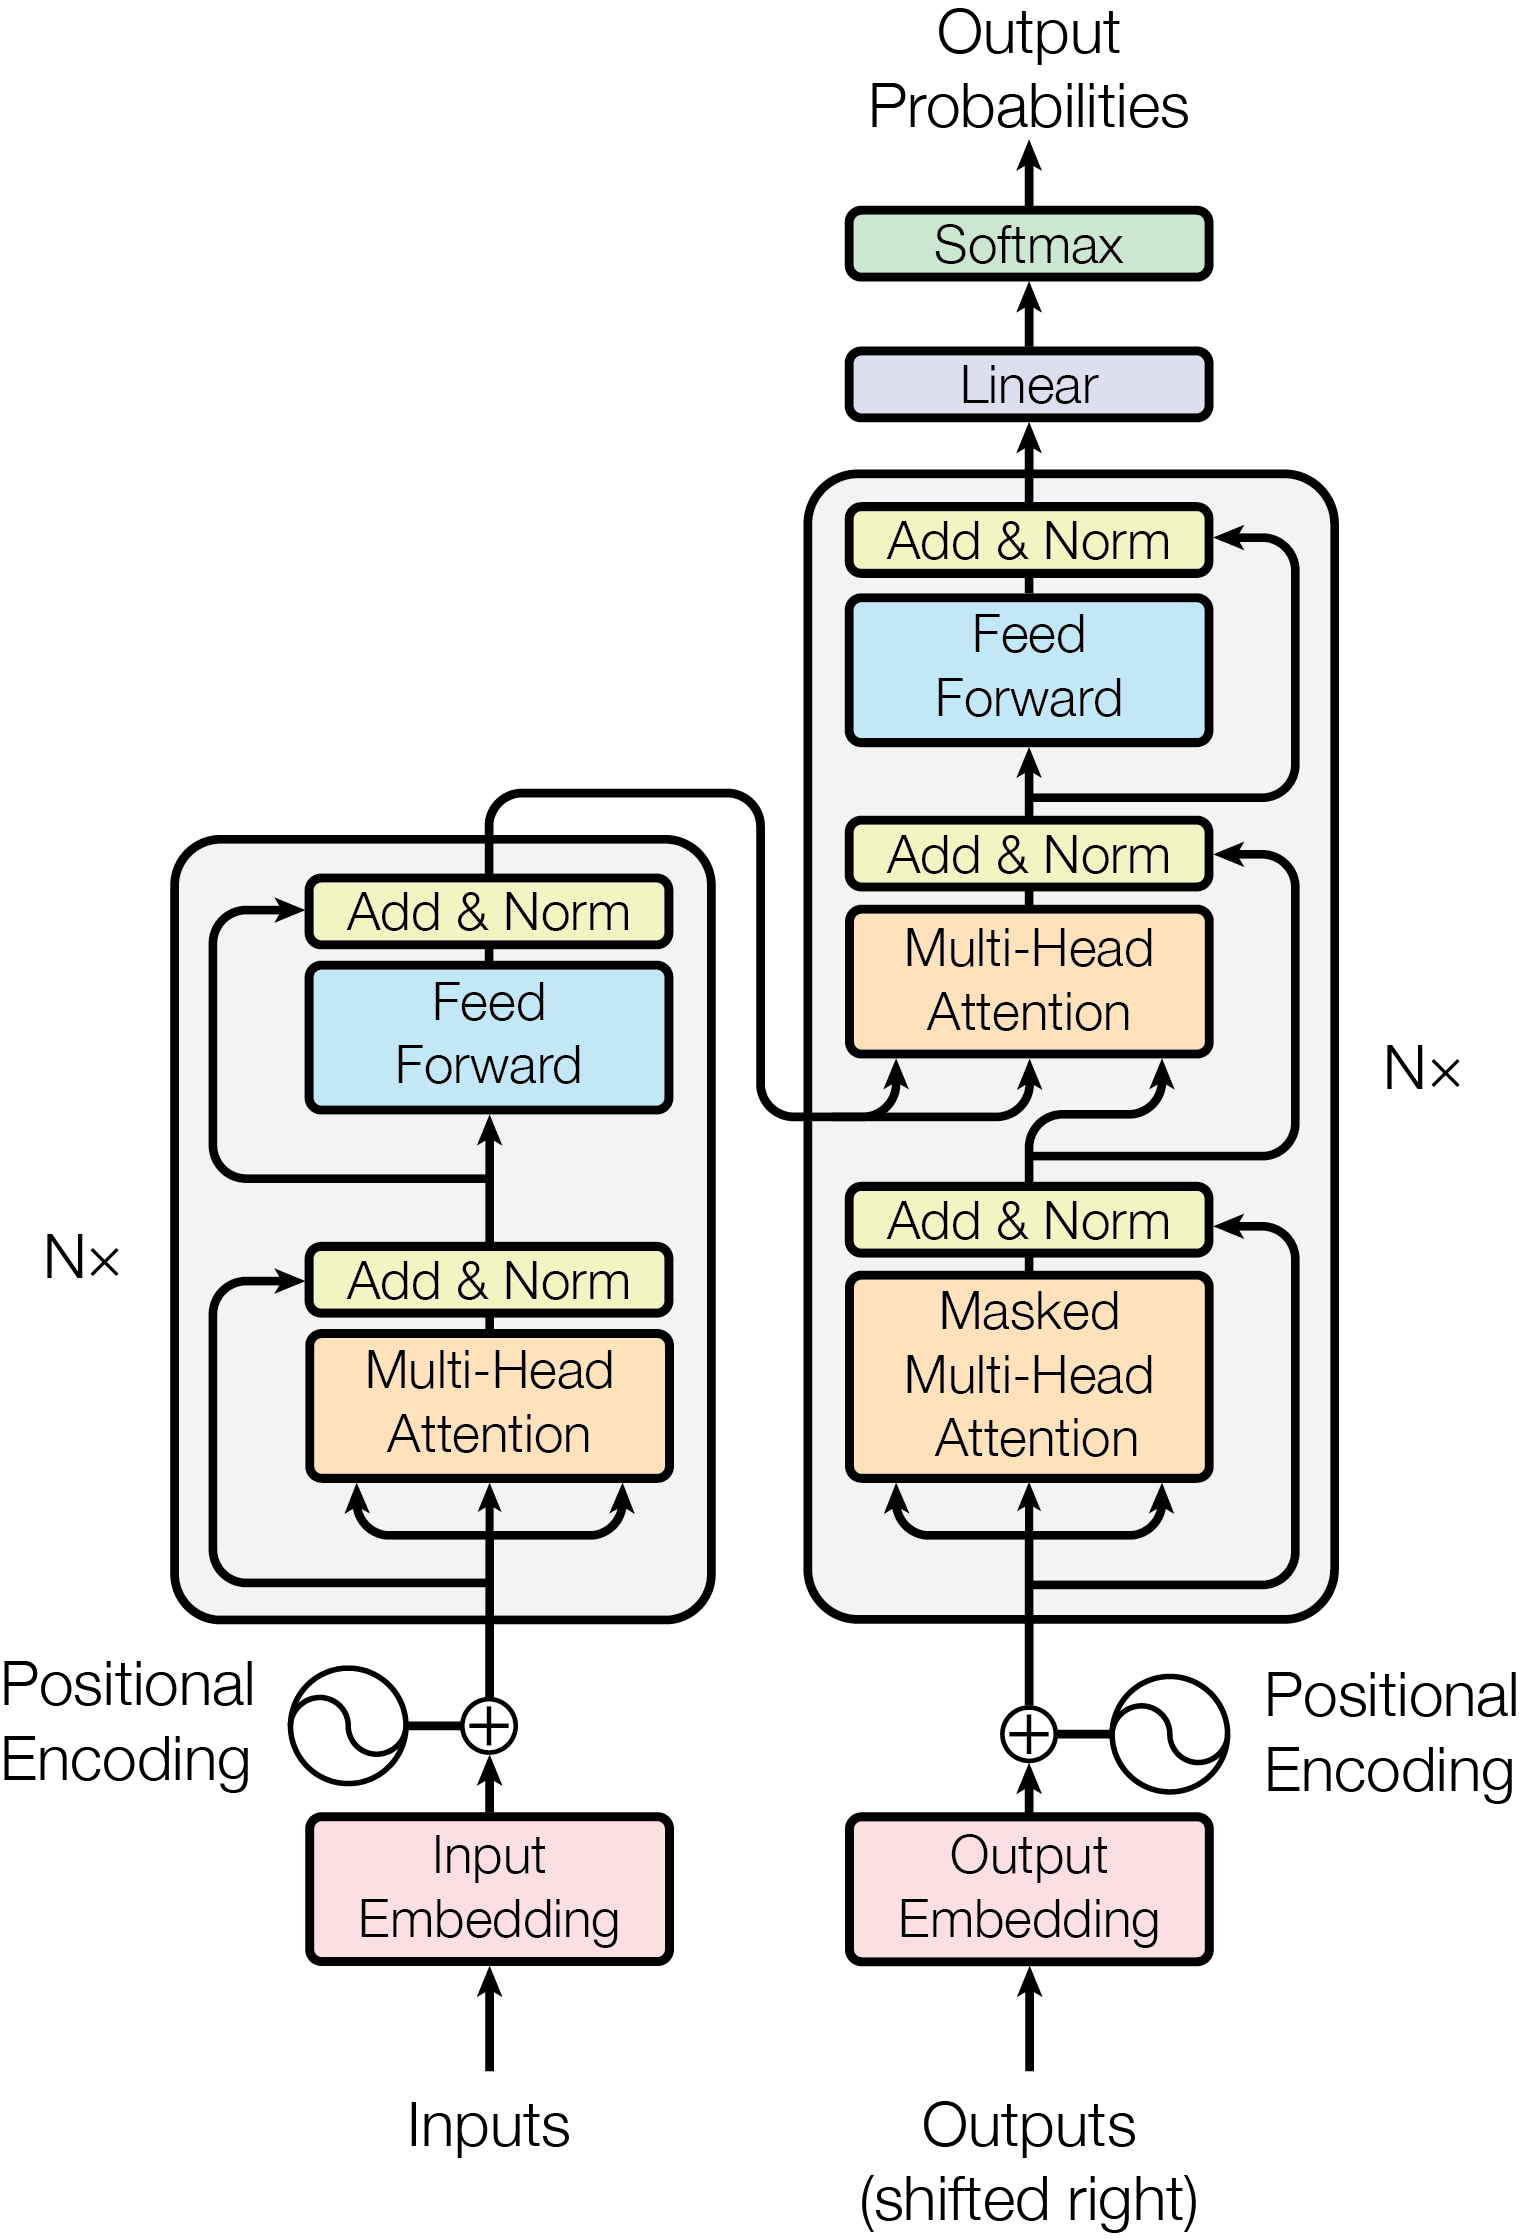
\includegraphics[width=0.6\textwidth]{figures/ModalNet-21.png}
%     \caption{Transformer model architecture \cite{NIPS2017_3f5ee243}}
%     \label{fig_transformers}
% \end{figure}

Transformers employ attention mechanisms to capture dependencies between words in a sequence, allowing them to understand and generate text with greater contextual awareness \cite{NIPS2017_3f5ee243}. The architecture of transformers, characterized by their extensive layers and attention mechanisms, necessitates vast amounts of parallel computation, making them an ideal fit for GPU acceleration.

GPUs excel at handling the matrix multiplications and element-wise operations inherent in the forward and backward passes of transformer models, leveraging their massively parallel architecture to accelerate training and inference processes. Moreover, the large memory bandwidth of GPUs helps process the immense datasets typically associated with LLMs efficiently, which enables scalability. As a result, integrating GPUs in LLM frameworks enhances computational performance. It allows researchers and practitioners to explore more complex models and larger datasets, pushing the boundaries of natural language understanding and generation. 

However, due to the highly intensive model structure and the complicated nature of distributed parallel training and inference logic, those generative AI training programs and inference applications will likely not utilize all the GPUs fully. GPU monitoring and alerting can provide insights into the performance and help identify code bugs and optimization opportunities for AI workloads, thus advancing state-of-the-art AI research and applications.

\subsection{Sustainability}

In HPC environments, GPUs are typically allocated by the device, while the CPU allocates cores. For instance, the LUMI supercomputer, ranked as the fastest in Europe according to TOP500 by December 2023 \cite{TOP500}, uses the AMD Radeon Instinct MI250X GPU Accelerator, which is equipped with 220 compute units (cores), in contrast to the 64-core 3rd Gen EPYC 7A53s Trento CPU \cite{lumi}. While this abundance of cores enables GPUs to efficiently manage numerous mathematical and spatial computations simultaneously, it also makes GPUs the most power-intensive component in a computing system.

Compared with CPUs, inefficient utilization of GPUs can lead to substantial resource wastage, particularly during peak hours when numerous jobs await allocation. As is shown in Table \ref{tab:lumi_resources}, the maximum TDP for the CPU is 280W \cite{amd-epyc-cpu}, whereas the TBP for the GPU is 500W, peaking at 560W \cite{amd-mi250x}. Thus, each allocation on systems like LUMI incurs a mere 4W per core for CPUs, contrasting wildly with the over 250W consumption for GPUs (1 GPU has 2 GCDs in this case here) \cite{lumi}.

\begin{table}[H]
    \centering
    \begin{tabular}{|c|c|c|c|c|c|}
        \hline
        Device & Cores & Maximum Power & Allocable & Allocation Power \\
        \hline
        GPU & 220 & 560W & 2 & 280W \\
        \hline
        CPU & 64 & 280W & 64 & 4.375W \\
        \hline
    \end{tabular}
    \caption{Resources comparison of GPU and CPU for LUMI}
    \label{tab:lumi_resources}
\end{table}

However, knowing the performance and getting alerted for sub-optimal jobs on time poses a challenge for supercomputer administrators. Existing workload managers and job schedulers in HPC systems, such as Slurm and LSF, provide descriptive accounts of CPU and memory usage but lack real-time hardware monitoring capabilities at the job level, and they have no accounting for GPU. They also have no built-in alert systems. As a result, a GPU monitoring and alerting system is urgently needed to help administrators ensure sustainability and reduce carbon emissions. Users may also need this information to debug/improve their code and make their program more environmentally friendly.

\section{Research questions}

By the time we started the thesis, a monitoring system for GPU had already been ready as part of the work during my 2023 summer internship at CSC -- IT Center for Science. As a result, this thesis aims to impact the above areas by implementing an alert service based on our existing monitoring system for supercomputers at CSC. It seeks to address the following research question:

\textbf{
How do we systematically design a service that efficiently and reliably analyzes jobs using GPUs in HPC systems in real-time?
}

This can be divided into the following sub-research questions:

\begin{itemize}
    \item \textit{How to minimize the alert delay with a fix-size window in real-time context?}

This involves exploring efficient methods to streamline detecting and responding to anomalies or critical events promptly.

    \item \textit{How to minimize the performance impact on the database systems?}

This includes optimizing database queries, resource allocation, or employing caching mechanisms to ensure minimal disruption to overall system performance.

    \item \textit{How to reliably maintain a data structure for job alert status check?}

This involves data organization, scalability, and fault tolerance to ensure reliable operation under varying workload conditions.
    
    \item \textit{How to find the most reliable algorithm for generating alerts?}

This includes assessing different algorithms' accuracy, efficiency, and scalability to determine their suitability for real-time alert generation in HPC environments.

\end{itemize}


\section{Contributions}

The contributions of this thesis are as follows:

\begin{itemize}
    \item We have successfully created and deployed the monitoring system and the alert service for Nvidia and AMD GPUs at job level with Slurm on supercomputer systems.
    \item Through an in-depth investigation of the collected monitoring data, an algorithm has been developed to identify and alert jobs with inefficient GPU resource usage. This achievement not only enhances the effectiveness of the alert service but also contributes to optimizing resource utilization and improving overall system efficiency.
    \item By analyzing the collected monitoring data and identifying patterns of inefficient GPU usage, this thesis contributes to a deeper understanding of resource utilization changes and patterns within HPC environments. This knowledge can inform future research and development efforts to optimize GPU-accelerated computing and improve the performance of AI workloads on supercomputers.
\end{itemize}

\section{Thesis structure}

In this thesis, we systematically explore techniques and methodologies for designing and implementing a monitoring system and alert service for GPU resource utilization on HPC clusters. Following the introduction, which provides background information, outlines the application domains, and presents research questions and contributions, the thesis is organized as follows:

Section 2 focuses on the background, which discusses various techniques for building the monitoring system and the alert service. This includes an examination of job schedulers, an overview of HPC systems at CSC (including Puhti, Mahti, and LUMI), an exploration of different monitoring systems such as /proc, Cgroups, NVML, and ROCm-SMI, database techniques including LISTEN \& NOTIFY, triggers, and continuous aggregates, as well as an overview of the time-series database TimescaleDB. Additionally, the section delves into alert algorithms, covering descriptive statistics, K-Means clustering and silhouette analysis, decision trees, and random forests.

Section 3 details the methods we use for the research, covering aspects such as implementing a monitoring system, alert service, and algorithms. This includes developing a monitoring daemon, timescale ingest, timescaleDB, timescale reader, alert algorithms, alert service, and alert dashboard.

In Section 4, benchmark results from both experimental and production setups are presented and analyzed. This includes an overview of the experimental setup, benchmarking results, and insights from production environments by case study.

Section 5 discusses the findings, analyzing related work and their implications and limitations.

Finally, Section 6 provides concluding remarks, including a summary of critical points and suggestions for future work.

\clearpage
%!TEX root = ../Thesis.tex
\chapter{Background}
\label{chap:background}
\section{Job scheduler}
\label{Sec:jobScheduler}
This Chapter briefly overviews the well-known open-source workload manager we use at CSC -- IT Center for Science, Slurm \cite{10.1007/10968987_3}.

Let's first start with some definitions:

\begin{enumerate}
    \item \textbf{Resource Manager} is a software component for overseeing the resources within a cluster, typically under the control of a scheduler. Its responsibilities include:

    \begin{itemize}
        \item Management of various resources such as nodes, CPUs, GPUs, memory, and network.
        \item Coordination of job execution across compute nodes to ensure efficient resource utilization.
        \item Prevention of resource overlap among concurrent jobs.
    \end{itemize}
    \item \textbf{Scheduler} is a software module that manages user jobs within a cluster based on predefined policies. It interacts with users to receive and handle new jobs while controlling the Resource Manager. Key features of a Scheduler include:

    \begin{itemize}
        \item Provision of partitions, queues, and Quality of Service (QoS) settings to enforce policies and limits on job execution.
        \item Implementation of scheduling mechanisms such as backfilling, first-in-first-out (FIFO), etc.
        \item Provision of interfaces for defining job workflows (e.g., job scripts), specifying job dependencies, and issuing commands for job management (e.g., submission, cancellation, etc.).
    \end{itemize}

    \item \textbf{Batch-System} or \textbf{Workload Manager} is the combination of a scheduler and a resource manager, combining the features of both components to manage workload within the cluster efficiently.
\end{enumerate}

% Slurm is vital in orchestrating parallel computing environments, bridging the gap between users and computational resources. At its core, Slurm embodies the roles of a resource manager and a job scheduler. The resource manager is the key, facilitating the execution of parallel jobs across distributed computing nodes. In contrast, the job scheduler dynamically allocates and manages resources to efficiently handle a queue of pending tasks, employing sophisticated scheduling algorithms optimized for various criteria such as network topology, fair-share scheduling, and advanced reservations.

Slurm, initially known as the Simple Linux Utility for Resource Management, emerged in 2002 at Lawrence Livermore National Laboratory as a batch system tailored for Linux clusters. As HPC environments require sophisticated workload managers to efficiently manage and allocate computing resources among multiple users and tasks, it evolved into a sophisticated scheduling framework incorporating advanced plugins.

% Today, Slurm is a robust system. Renowned for its scalability, It has been deployed on most of the world's largest computing systems, catering to diverse computational needs across various domains.

% Designed with scalability in mind, Slurm prides itself on its ability to manage colossal systems. As an open-source software under the GPLv2 (GNU General Public License version 2), Slurm promotes accessibility and fosters an active global development community. Its system administrator-friendly interface, coupled with its emphasis on security and fault tolerance, renders it a favored choice among administrators.

The architecture of Slurm is modular and extensible, with many plugins available to cater to diverse requirements. At the core of Slurm, we have mainly the following three components:

\begin{itemize}
    \item \textbf{Slurmctld} serves as the central management daemon within the Slurm framework, orchestrating the activities of all other Slurm daemons and resources. Its primary functions include the monitoring of system resources and the allocation of these resources to incoming workloads (jobs). Additionally, Slurmctld is a connecting point for accepting and processing job submissions, ensuring efficient utilization of available computing resources.
    \item \textbf{Slurmdbd} offers a secure and centralized interface to interact with the database system, specifically tailored to cater to the needs of Slurm. This daemon enables features such as archiving accounting records and storing essential metadata related to job executions. It ensures the integrity and confidentiality of data while providing seamless access to critical information for administrative and analytical purposes.
    \item \textbf{Slurmd} functions as the compute node daemon, operating at the node level to oversee the execution of computational tasks. Among its key responsibilities, slurmd actively monitors the status of tasks running on the compute nodes, facilitating efficient task management and resource allocation. It also acts as a connecting point for receiving task assignments, launching tasks onto the compute nodes, and terminating tasks as per system requirements or user requests.
\end{itemize}

Slurm plays a crucial role in maximizing the utilization of computational resources and ensuring fair access for users to run their parallel and distributed applications. It offers a powerful yet flexible solution for managing and scheduling computational workloads. Slurm is a preferred choice for orchestrating complex computing infrastructures worldwide, as used by over 65\% of TOP500 systems \cite{aboutslurm}.

% \subsection{LSF}
% IBM Spectrum LSF is a comprehensive workload management platform that handles complex scheduling and resource management in HPC environments. LSF supports various applications, from serial jobs to parallel and distributed computing tasks. It efficiently allocates resources based on priority, policies, and system constraints.

% Key features of LSF include:
% \begin{itemize}
%     \item \textbf{Dynamic Resource Allocation}: LSF can dynamically allocate resources based on the changing workload, optimizing resource utilization.
%     \item \textbf{Job Prioritization}: LSF allows users to set job priority levels, ensuring critical tasks get precedence.
%     \item \textbf{Job Arrays}: LSF supports job arrays, enabling users to submit related jobs as a single entity.
%     \item \textbf{Prolog and Epilog}: LSF allows users to define Prolog and Epilog scripts that run before and after job execution, respectively. Prolog scripts prepare the environment, while Epilog scripts handle cleanup tasks.
% \end{itemize}

% There are also some minor differences between LSF and Slurm:

% \begin{enumerate}
%     \item \textbf{Architecture}:
%     \begin{itemize}
%         \item \textit{LSF}: Proprietary software developed by IBM.
%         \item \textit{Slurm}: Open-source software with a community-driven development model.
%    \end{itemize}

%     \item \textbf{Configuration}:
%     \begin{itemize}
%         \item \textit{LSF}: Configurable with a comprehensive set of parameters.
%         \item \textit{Slurm}: Known for its simple and straightforward configuration.
%     \end{itemize}

%     \item \textbf{Resource Allocation}:
%     \begin{itemize}
%         \item \textit{LSF}: Dynamically allocates resources based on workload changes.
%         \item \textit{Slurm}: Offers flexibility with partitioning and node affinity settings.
%     \end{itemize}

%     \item \textbf{Job Priority}:
%     \begin{itemize}
%         \item \textit{LSF}: Users can set priority levels for jobs.
%         \item \textit{Slurm}: Utilizes Quality of Service (QoS) for defining job execution policies.
%     \end{itemize}
% \end{enumerate}

\section{HPC systems at CSC}
\label{sec:hpc}
Table \ref{tab:gpu_details} shows the GPU statistics for the three HPC systems at the CSC-IT Center for Science: Puhti, Mahti, and LUMI. Understanding the architecture and capabilities of these systems is crucial for tailoring GPU monitoring and alerting strategies and ensuring seamless integration with existing infrastructure. This Section provides an overview of the GPU computing nodes for these HPC systems.

\begin{table}[H]
    \centering
    \begin{tabular}{|c|ccc|}
     \hline
     \textbf{Item} & \textbf{Puhti} & \textbf{Mahti} & \textbf{LUMI} \\
     \hline
     \textbf{Number of GPU nodes} & 80 & 24 & 2928 \\
     \hline
     \textbf{GPU Model} & Nvidia V100 & Nvidia A100 & AMD MI250X \\
     \hline
     \textbf{GPU number per node} & 4 & 4 & 4 / 8 (GCDs) \\
     \hline
     \textbf{Total number of GPUs} & 320 & 96 & 11712 / 23424 (GCDs) \\
     \hline
    \end{tabular}
    \caption{GPU statistics for HPC systems at CSC -- IT Center for Science}
    \label{tab:gpu_details}
\end{table}

\subsection{Puhti}
Puhti \cite{puhti} is an Atos BullSequana X400 cluster. Its AI partition comprises 80 GPU nodes, tailored specifically for artificial intelligence tasks, and collectively achieve a peak performance of 2.7 petaflops. Each node integrates the Intel Xeon Gold 6230 processors of the Cascade Lake family, which has 20 cores running at 2.1 GHz and supports AVX-512 vector instructions \& VNNI instructions for AI inference workloads. We have a total thread count of 80 threads per node (40 per socket). Additionally, we have 4 Nvidia Volta V100 GPUs on each node, each with 32 GB of memory and connected via NVLink. Each node also features 384 GB of main memory and 3.6 TB of high-speed local storage.

\subsection{Mahti}

Mahti \cite{mahti} is an Atos BullSequana XH2000 cluster. It comprises 24 GPU nodes, accumulating a theoretical peak performance of 2.0 petaflops. Each CPU and GPU node has 2 AMD Rome 7H12 CPUs featuring 64 cores each. The CPUs are based on the AMD Zen 2 architecture and operate at a base frequency of 2.6 GHz and a maximum peak frequency of up to 3.3 GHz. They also support the AVX2 vector instruction set. Each core supports simultaneous multi-threading, enabling 256 threads per node.

The GPU nodes have 512 GB of memory and a local 3.8 TB NVMe drive. They also have 4 Nvidia Ampere A100 GPUs, with a subset of nodes featuring split A100 GPUs, which enable lightweight workloads such as interactive tasks, courses, and code development and save energy consumption.

\subsection{LUMI}
\label{subsec:lumi}
By Jun 2024, LUMI \cite{lumi}, one of the three European pre-exascale supercomputers and an HPE Cray EX supercomputer, was the fastest supercomputer in Europe. The GPU partition, LUMI-G, features the primary compute power, which consists of 2978 nodes, as described in Figure \ref{fig_lumig_overview}.

\begin{figure}[H]
    \centering
    \includesvgpath[width=0.9\textwidth]{lumig-overview.svg}
    \caption{LUMI GPU partition overview \cite{lumi}}
    \label{fig_lumig_overview}
\end{figure}

\subsubsection{GPU}

The LUMI-G compute nodes have four AMD MI250X GPUs, each based on the 2nd Gen AMD CDNA architecture. The MI250X GPU is structured as a multi-chip module, which includes two GPU dies referred to as AMD Graphics Compute Dies (GCD). In Slurm and HIP runtime, a single MI250X module is recognized as two GPUs. Thus, in the actual system, the LUMI-G are 8-GPU nodes.

Each GCD has 110 compute units and accesses a 64 GB slice of high-bandwidth memory, totaling 220 compute units and 128 GB of memory per MI250X module. All compute units share an L2 cache with an 8 MB capacity to enhance memory throughput. The cache is divided into 32 slices, capable of delivering 128 B/clock/slice, amounting to a peak theoretical bandwidth of 6.96 TB/s. Including an L2 cache in the MI250X GPU modules enhances synchronization capabilities for algorithms reliant on atomic operations to coordinate communication across the entire GPU. These atomic operations are executed close to the memory within the L2 cache.

\subsubsection{CPU}

The CPU of LUMI-G nodes is a 64-core AMD EPYC 7A53 Trento CPU. These CPU cores, built on the Zen 3 architecture, support AVX2 256-bit vector instructions, enabling a maximum throughput of 16 double-precision FLOP/clock (AVX2 FMA operations). Each core has 32 KiB of private L1 cache, a 32 KiB instruction cache, and 512 KiB of L2 cache. The L3 cache has 32 MiB shared among groups of 8 cores, accumulating 256 MiB of L3 cache per CPU. Configured as 4 NUMA nodes (NPS4), the system allocates 128 GiB of DDR4 memory per NUMA node, resulting in 512 GiB of CPU memory.

\section{Monitoring tools}
A robust selection of monitoring techniques is crucial for capturing accurate metrics, diagnosing performance issues, and ensuring efficient resource utilization. This Section explores various components for building a monitoring system, each offering unique capabilities for monitoring within large-scale distributed computing clusters. Thus, it provides the cornerstone for building an accurate alert algorithm.

\subsection{Cgroups}
Cgroups \cite{7876184} is a Linux kernel feature that enables the isolation and accounting of resources, including CPU, memory, and devices, among a collection of processes. It provides a means to track and manage CPU and memory utilization per process.

Slurm can be configured to use Cgroups to regulate resources allocated to jobs, steps, and tasks and for resource accounting. Cgroups have different controllers (subsystems), each responsible for managing specific resources. Slurm's plugins can utilize multiple controllers, including memory, CPU, devices, freezer, cpuset, and cpuacct. Each enabled controller empowers Slurm to enforce resource constraints on a defined set of processes. Slurm cannot enforce resource constraints through Cgroups for the associated resources if a controller is unavailable. Slurm supports two Cgroup modes through plugins: Legacy mode (Cgroups v1) and Unified Mode (Cgroups v2, introduced in Linux Kernel version 5.8).

% Compared with Cgroup v1, Cgroup v2 introduces several enhancements, including:
% \begin{itemize}
%     \item \textbf{Unified Hierarchy Design}: Cgroup v2 adopts a single unified hierarchy structure within the API, simplifying management operations.
%     \item \textbf{Enhanced Container Delegation}: It provides a safer delegation of sub-trees to containers, ensuring improved isolation.
%     \item \textbf{Integration of New Features}: Cgroup v2 incorporates newer features like Pressure Stall Information (PSI), enhancing resource monitoring capabilities.
%     \item \textbf{Improved Resource Management}: It offers refined resource allocation and isolation across multiple resource types, enhancing system performance.
%     \item \textbf{Unified Memory Accounting}: Cgroup v2 uses unified accounting for various memory allocations, including network and kernel memory.
%     \item \textbf{Handling Non-Immediate Resource Changes}: It introduces support for accounting non-immediate resource changes, such as page cache write-backs.
% \end{itemize}

At CSC, Puhti and Mahti still use Red Hat Enterprise Linux (RHEL) 8, which means Cgroup v1. In contrast, LUMI uses a more recent system, SUSE Linux Enterprise Server (SLES) 15 SP4, which means Cgroup v2. So, we need to support both Cgroup versions to cover the CPU and memory monitoring for all the systems.

Cgroups can form the foundation for understanding CPU and memory consumption. Take Cgroups v1, for example:

\begin{itemize}
    \item \textbf{/sys/fs/cgroup/memory/slurm/uid\_*/job\_*/*/memory.usage\_in\_bytes} tells the memory usage for the job.
    \item \textbf{/sys/fs/cgroup/cpuset/slurm/uid\_*/job\_*/cpuset.cpus} tells the list of CPU cores that are used by the job.
\end{itemize}

\subsection{/proc}
The /proc \cite{5544096} directory is unique within the Linux file system, as it functions as a virtual filesystem. Often described as a process information pseudo-file system, it diverges from traditional directories by not containing actual files of the same size since these files serve as pointers, directing users to the underlying location of process information within the kernel. Thus, it provides runtime system data such as system memory utilization, mounted devices, and hardware configurations.

% The /proc serves as a hub for kernel control and information dissemination -- many system utilities directly access files within this directory to gather essential system data. For instance, commands like \texttt{lsmod} and \texttt{lspci} are essentially shorthand for \texttt{cat /proc/modules} and \texttt{cat /proc/pci}, respectively. Furthermore, modifying files within /proc enables users to interact with kernel parameters, facilitating real-time adjustments to system configurations via sysctl.

% A distinctive characteristic of files within /proc is, that they almost all have a file size of 0, with exceptions like kcore, mtrr, and self.

When browsing the directory, we see those numbered subdirectories corresponding to the unique process ID (PID). By cross-referencing these PIDs with the process table, we can identify and examine specific processes. For instance, if the process table denotes a process with PID 1234, accessing the directory /proc/1234 reveals detailed information about this process.
    
The /proc can also form the basis for understanding CPU and memory consumption. Monitoring processes often involve parsing information from /proc to extract consumption-related statistics according to process IDs, including their memory usage and CPU information:

\begin{itemize}
    \item \textbf{/proc/cpuinfo} helps us know the frequency of CPU cores in the current node.
    \item \textbf{/proc/<PID>/status} helps us know how many CPU cores we got allocated, as well as the current Resident Set Size (RSS) and max RSS, which is the maximum amount of memory used at any time by the process in that job context.
    \item \textbf{/proc/<PID>/maps} provides information about memory mappings for the specified process. It includes a list of memory regions allocated to the process and details such as the starting and ending addresses, permissions, and file mappings, if applicable.
\end{itemize}

\subsection{GPU management library}
\subsubsection{NVML}
NVML \cite{nvml} is a GPU-specific library provided by NVIDIA for managing and monitoring NVIDIA GPU devices. Its C-based API is designed to monitor and control the diverse states of NVIDIA GPU devices. This API offers direct access to the queries and commands accessible through Nvidia-SMI. It can help efficiently manage and monitor NVIDIA GPU devices. NVML exposes a comprehensive set of metrics, including GPU temperature, memory usage, and GPU utilization, allowing for detailed insights into GPU performance.

NVML is a cornerstone for GPU monitoring on systems equipped with NVIDIA GPUs, such as Puhti and Mahti.

\subsubsection{ROCm-SMI}
ROCm-SMI \cite{rocm-smi} is an analogous tool to NVML but tailored for AMD GPUs within the Radeon Open Compute ecosystem. Like NVML, ROCm-SMI provides GPU-specific metrics, allowing for the monitoring and managing of AMD GPU devices.

For HPC clusters that utilize AMD GPUs, such as LUMI, integrating ROCm-SMI into the GPU monitoring framework is essential. In contrast, Puhti and Mahti utilize NVIDIA GPUs, so NVML is used in these two systems.

\section{Time-series databases}

% This Section explores two prominent time-series databases, InfluxDB and TimescaleDB \cite{le2021developing}.

% \subsection{InfluxDB}
% InfluxDB is a high-performance, open-source time series database developed by InfluxData. It is written in Go and is optimized for handling time series data at scale, making it a popular choice for use cases involving monitoring performance metrics, IoT data, and real-time analytics.

% InfluxDB is more than just a time series database. It also includes the InfluxDB User Interface (InfluxDB UI) and Flux, a functional scripting and query language that enables sophisticated data transformation.

% InfluxDB 3.0 \cite{10.1007/978-3-031-42529-5_26}, the newest version of InfluxDB, is built in Rust, a modern programming language designed for performance, safety, and memory management. It features a decoupled architecture that allows computing and storage to be scaled independently. InfluxQL is an SQL-like query language that replaces Flux for working with data in InfluxDB databases.

% \subsection{TimescaleDB}
Time-series data management is a critical aspect of data lifecycle management, mainly due to its complexities. Time-series data, comprising a sequence of data points recorded over discrete time intervals, provides invaluable insights into evolving phenomena spanning milliseconds to years. Widely applicable across various domains, time-series data uses time as the principal axis for data organization.

Effectively managing time-series data involves addressing numerous challenges, ranging from efficient data ingestion to optimized query performance and cost-effective resource utilization. Time-series databases play a pivotal role in storing and analyzing time-stamped data efficiently. Choosing the right time-series database is crucial for managing and querying the vast amount of data generated by monitoring metrics, thus contributing to resolving \textbf{RQ1} in Section \ref{sec:rqs}.

One of the primary challenges in time-series monitoring for HPC jobs is handling high cardinality, which refers to the number of unique sets of data combinations. High cardinality can lead to performance bottlenecks as the database needs to manage and index many unique series, each potentially requiring separate storage and processing resources. This can strain the database system's capacity to ingest data rapidly and execute queries efficiently, especially as the data volume scales. Many non-time-series databases, and other time-series databases, including InfluxDB, will crash as the job to record (cardinality) increases.

\subsubsection{TimescaleDB}

TimescaleDB \cite{timescaledb} emerges as a robust solution, excelling in both rapid data ingestion and streamlined query processing, ensuring comprehensive time-series data management capabilities. TimescaleDB is an open-source time-series database optimized for fast ingest and complex queries. It is engineered on top of the mature RDBMS system PostgreSQL and packaged as an extension. TimescaleDB extends PostgreSQL with time-series-specific optimizations and functions, allowing it to manage time series data efficiently. TimescaleDB supports the full range of SQL functionality, including aggregates, joins, subqueries, and window functions.

Central to TimescaleDB's architecture are \textbf{hypertables}, which serve as fundamental structures for efficient time-series data management as shown in Figure \ref{fig:hypertables-chunks}. Hypertables abstract multiple individual tables that store the data, referred to as chunks, providing users with a unified interface for data interaction. With hypertables, users can execute diverse operations, including data insertion, querying, and schema modifications, seamlessly integrating standard SQL functionalities. Hypertables are particularly advantageous for time-series data management, because they efficiently partition incoming data into smaller, manageable subsets. These data subsets, represented as time-based chunks, enable TimescaleDB to efficiently handle data retention and optimization. Consequently, TimescaleDB can do fast data ingestion and is scalable to ions of rows per second, which is crucial for time-series applications.

\begin{figure}[H]
\centering
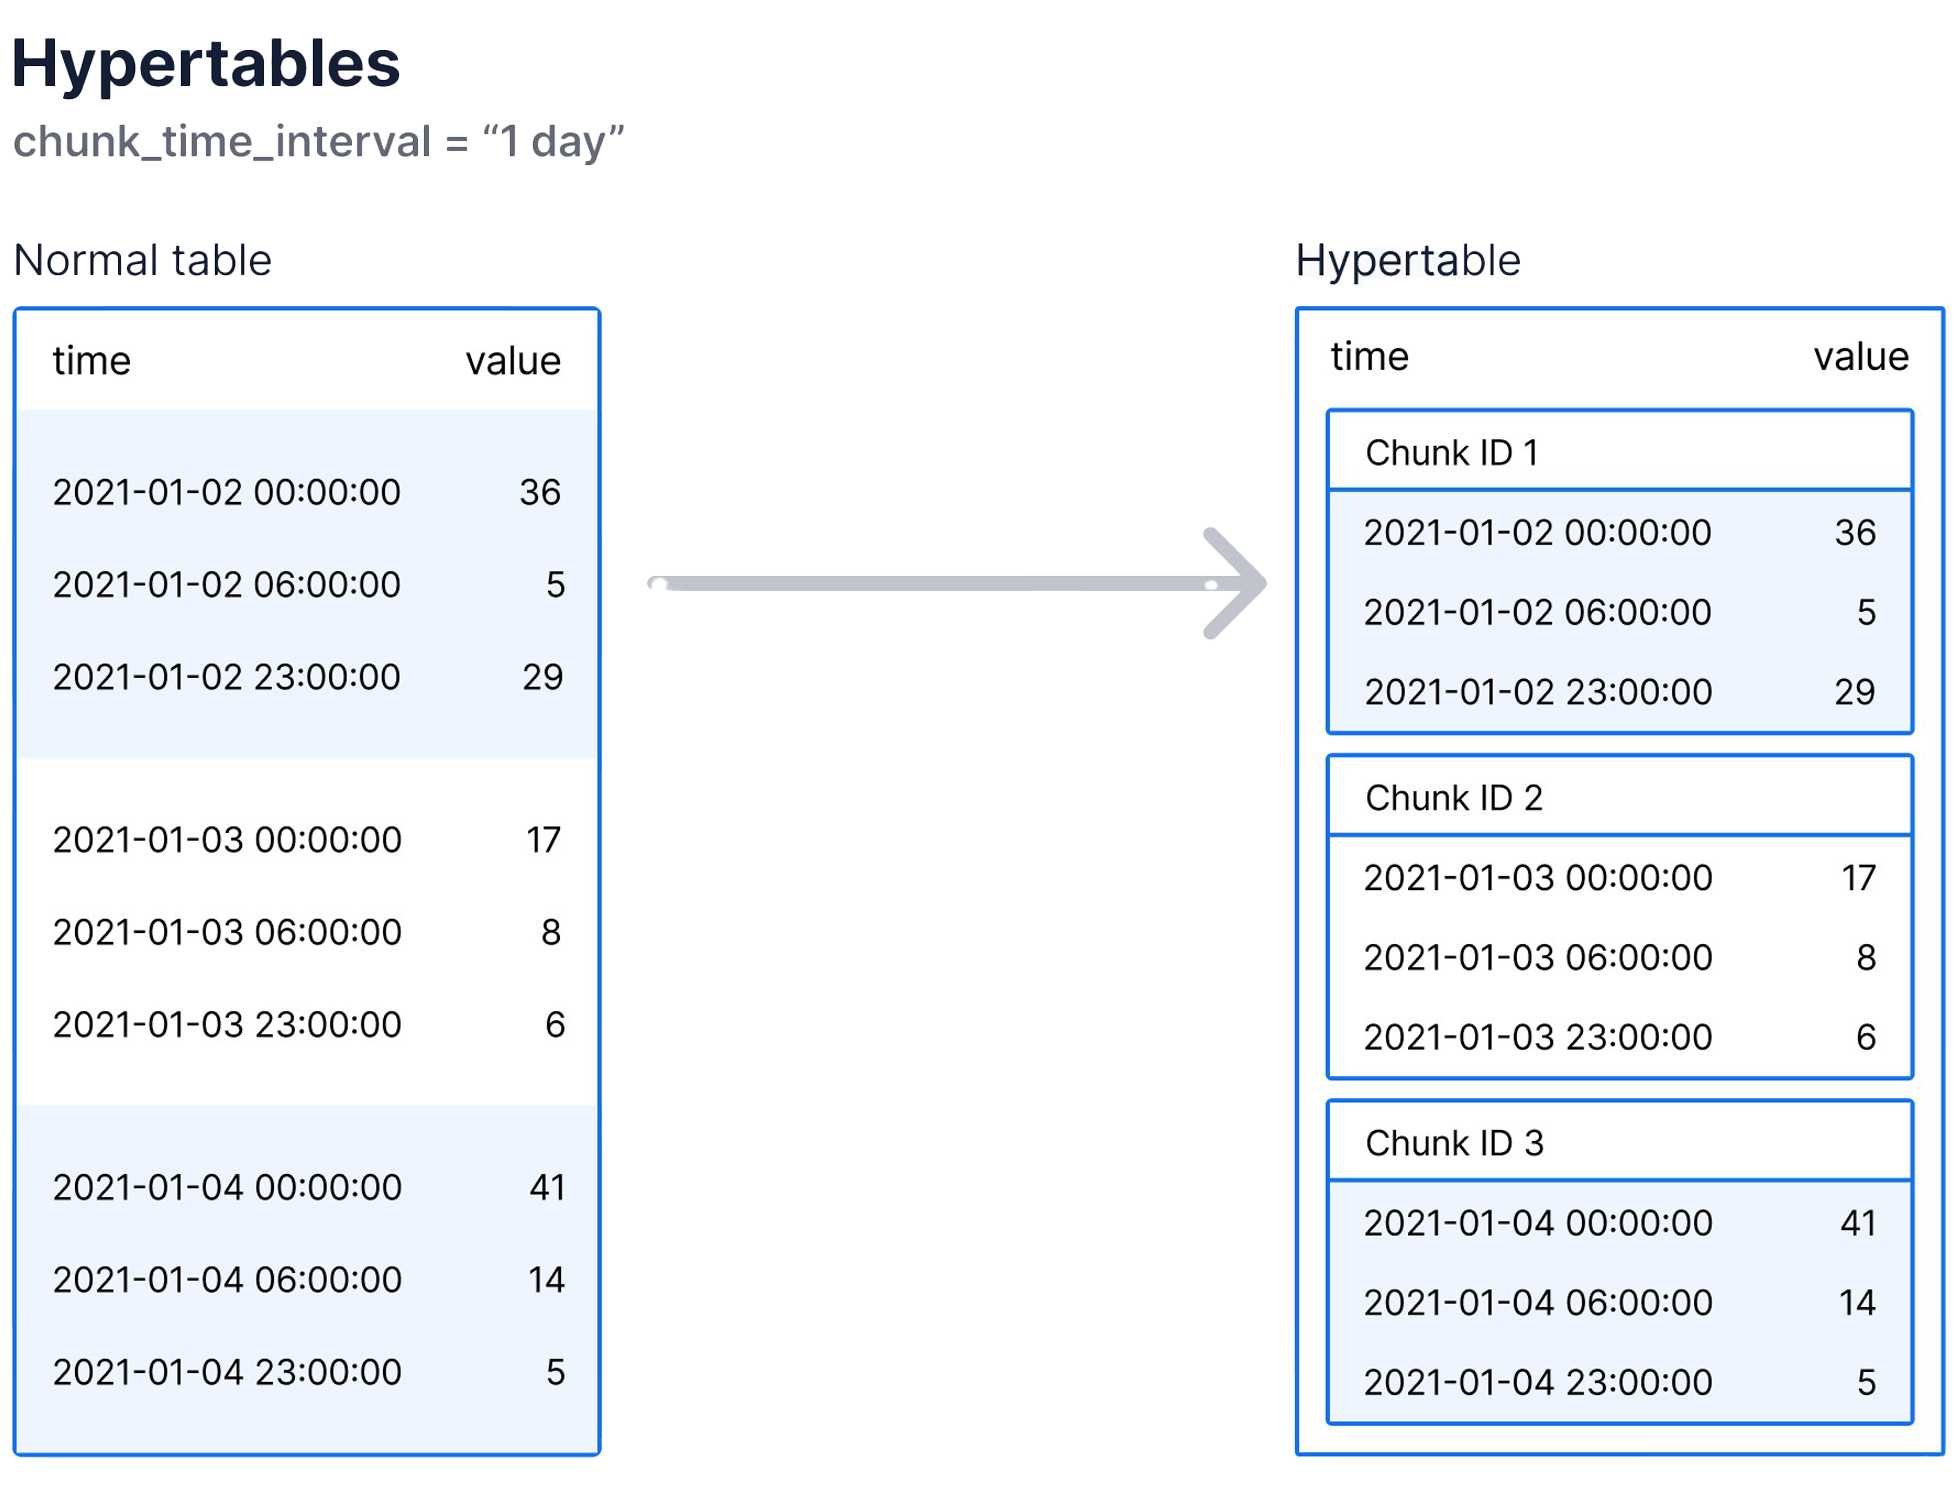
\includegraphics[width=0.9\textwidth]{figures/hypertables-chunks.png}
\caption{Hypertable compared with normal table \cite{hypertables}}
\label{fig:hypertables-chunks}
\end{figure}

Moreover, TimescaleDB effectively addresses cardinality issues. Leveraging hypertables and their automatic partitioning mechanism minimizes the overhead of managing high-cardinality data sets. This partitioning ensures the data is distributed across smaller chunks, reducing the performance impact when querying large datasets and maintaining efficient indexing.

\textbf{Compression} functionalities in TimescaleDB further enhance data storage efficiency. By employing compression algorithms such as delta encoding, delta-of-delta, simple-8b, run-length encoding, etc. \cite{timescaledb-compress}, TimescaleDB significantly reduces disk space utilization, achieving very high compression ratios.

TimescaleDB also facilitates the implementation of \textbf{data retention} policies as background jobs, automating the removal of obsolete data chunks and ensuring efficient data lifecycle management.

These features collectively make TimescaleDB a preferred choice over other time-series databases, especially for applications requiring robust performance under high cardinality conditions.

\section{Database techniques}
Databases are crucial in effectively managing and analyzing time-series data generated in real-time GPU resource monitoring. Our motivation is to create a system that can handle long-term reliable storage and provide near real-time status overviews without heavy SQL searches, thus contributing to resolving both \textbf{RQ1} and \textbf{RQ2} in Section \ref{sec:rqs}. To achieve this, we explore three significant database techniques that can be employed: Triggers, LISTEN \& NOTIFY, and Continuous Aggregates.

\subsection{Triggers}

Triggers \cite{Shaik2023triggers, postgresql-doc} are database elements that automatically respond to specific events or changes in the database. In GPU resource monitoring, a trigger can be activated upon inserting new GPU monitoring data, instantly processing this data and notifying relevant services. This ensures that the data is immediately available for long-term storage and real-time monitoring, facilitating a seamless integration between the two tiers of data management.

% This includes sending notifications via NOTIFY, based on GPU metrics stored in the time-series database.

A trigger in database management serves as a specification, that executes a designated function automatically, whenever a particular type of operation is conducted. The function must be declared as accepting no arguments and returning type triggers. It is important to note, that the trigger function receives input via a specially passed TriggerData structure, rather than conventional function arguments. Triggers can be configured to execute before or after an INSERT, UPDATE, or DELETE operation on a per-row or per-statement basis. Upon occurrence of a trigger event, the designated trigger function is invoked at the appropriate time to handle the event.

PostgreSQL offers two distinct types of triggers: \textbf{per-row (row-level)} triggers and \textbf{per-statement (statement-level)} triggers. Per-row triggers invoke the trigger function once for each row affected by the triggering statement. Conversely, per-statement triggers are invoked only once, when the corresponding statement is executed, irrespective of the number of rows impacted by the statement. Statement-level triggers also lack a mechanism to examine the rows modified by the statement.

Triggers can further be categorized as \textbf{before} triggers or \textbf{after} triggers. Statement-level before triggers are inherently activated before the start of the relevant statement, while statement-level after triggers are triggered upon the end of the statement. On the other hand, row-level before triggers are activated immediately before an operation on a specific row, while row-level after triggers are triggered after the statement but before any statement-level after triggers.

% For per-statement triggers, the trigger functions should, in any case, return NULL. In contrast, trigger functions invoked by per-row triggers can return a table row (a value of type HeapTuple) to the invoking executor. Specifically, a row-level trigger fired before an operation offers the following possibilities:

% \begin{itemize}
%     \item Returning NULL to bypass the operation for the current row, thereby telling the executor to drop the row-level operation that triggered the invocation of the trigger.

%     \item For row-level INSERT and UPDATE triggers exclusively, the returned row assumes the role of the row to be inserted or the row being updated, offering the trigger function the opportunity to modify that row.
% \end{itemize}

% Row-level before triggers, that do not intend to have either of these behaviors must ensure that they return the same row passed in. The return value is disregarded for row-level triggers activated after an operation; hence, they may safely return NULL.

Typically, row-level before triggers are employed for data validation or modification before insertion or updating. Conversely, row-level after triggers are generally utilized to update other tables or perform consistency checks against other tables. This distinction is generated from the fact, that an after trigger can make sure that it is observing the final value of the row, whereas a before trigger cannot. Consequently, if there is no specific rationale for selecting between a before or after the trigger, the before the trigger is preferred for its efficiency, as information about the operation need not be retained until the end of the statement.

% In circumstances where multiple triggers are defined for the same event on a given relation, the related triggers are fired alphabetically by trigger name. In the case of before triggers, the potentially modified row returned by each trigger serves as input to the subsequent trigger. If any before trigger returns NULL, the operation is abandoned for that row, and subsequent triggers are not invoked. Should a trigger function execute SQL commands, these commands may, in turn, trigger additional triggers. This phenomenon, known as \textbf{cascading triggers}, imposes no direct limit on the number of cascade levels. However, trigger programmers must stop infinite recursion from happening in such scenarios.

% During trigger definition, arguments can be specified to facilitate the invocation of different triggers with similar requirements calling the same function. This enables the creation of a generalized trigger function capable of accommodating diverse requirements across multiple tables. The provision of arguments in the trigger definition allows the same function to be leveraged for INSERT events on any table with requisite columns, facilitating automatic tracking of record creation, for instance. Additionally, it can be employed to monitor last-update events if configured as an UPDATE trigger.

The input data within the trigger function includes the trigger event type (e.g., INSERT or UPDATE) and any specified arguments in the CREATE TRIGGER command. For row-level triggers, the input data consists of the NEW row for all types of triggers, and the OLD row for UPDATE and DELETE triggers precisely.

\subsection{LISTEN \& NOTIFY}

LISTEN \& NOTIFY mechanism \cite{Shaik2023listen, postgresql-doc} is a powerful feature in PostgreSQL that provides asynchronous event notification. This technique enables efficient communication between the monitoring infrastructure and other system components, such as the alert service. It helps avoid the overhead of continuous polling and heavy SQL searches, enhancing system efficiency and responsiveness. When a relevant event occurs, such as the arrival of new GPU metrics or job state changes, the NOTIFY command can trigger notifications to any components that have registered interest with the LISTEN command, providing near real-time status updates.

\textbf{LISTEN} command registers the current session as a listener on the notification channel specified by the parameter. All sessions currently listening on the notification channel receive notifications. As a result, each listening session can be notified of its associated client application. Listen registrations of a session are automatically cleared upon the termination of that session.

It is up to the underlying PostgreSQL application programming interface for the client application to detect notification events. For the PostgreSQL driver and toolkit (\textbf{pgx}) package in Golang, listening for notification is a blocking read operation on the underlying socket. It will allocate a connection exclusively for listening purposes, allowing it to be blocked indefinitely.

% For instance, with the libpq library, the application issues LISTEN as a conventional SQL command and periodically calls the PQnotifies function to make sure whether any notification events have been received. 

\textbf{NOTIFY} enables processes accessing a shared PostgreSQL database to exchange information. The data transmitted to the client during a notification event includes the name of the notification channel, the process ID (PID) of the notifying session's server, and the payload string, which defaults to an empty string if unspecified, to client applications previously registered in listening for events on a specified channel within the current database. These notifications are broadcast to all listeners. More complex data structures can be established with database tables, to convey additional information from the notifier to the listeners. 

A practical programming approach to signaling changes to a particular table using NOTIFY involves embedding the NOTIFY command within a trigger, triggered by table insertion.

% It is worth noting that notifications issued within a transaction are only dispatched upon transaction commitment, ensuring consistency in the event of transaction rollback. Notifications received during a transaction are deferred until after completion, to avoid premature delivery in case of a transaction abort.

% Duplicate notifications with identical payload strings within the same transaction deliver only one notification event to listeners. Conversely, notifications with distinct payload strings are treated as distinct events. Additionally, notifications from different transactions are always delivered in the order of transaction commitment, ensuring sequential delivery.

% Implementing LISTEN \& NOTIFY in the monitoring system enhances the responsiveness of the alert service, allowing it to receive notifications about new GPU metrics as they arrive instantly. This approach is precious in scenarios where timely reactions to changes in GPU resource utilization are crucial. By decoupling the notification mechanism from the traditional request-response model via polling, LISTEN \& NOTIFY contributes to the monitoring system's overall efficiency and real-time capabilities.

\subsection{Continuous aggregates}
% Continuous aggregates in TimescaleDB offer a reliable solution for analyzing time-series data trends, leveraging aggregate functions to observe temporal patterns effectively. Unlike traditional approaches, continuous aggregates intelligently update aggregated data, refreshing only relevant portions of chunks based on underlying data modifications. Consequently, continuous aggregates optimize historical query performance while serving as a long-term data repository independent of changes to raw data.

% Continuous Aggregates can contribute to optimizing data storage and query performance. By pre-computing aggregated values at regular intervals, the system can quickly retrieve summarized information for alerting and analysis. This approach ensures the monitoring system maintains responsiveness even as the time series data grows, providing administrators with timely insights into GPU resource utilization trends.

Time-series data tends to experience rapid expansion over time. Consequently, aggregating such data into meaningful summaries often encounters considerable latency. Continuous aggregates \cite{10.14778/3611540.3611559} offer a solution by fastening the data aggregation process.

In scenarios where data is collected at high frequencies, it becomes advantageous to aggregate the data into more considerable time intervals, such as minutes or hours. For instance, when GPU usage readings are recorded every second, computing the average GPU usage for each hour means we must scan the entire dataset and recalculate the average with each query execution. There are generally three ways to do the aggregation within TimescaleDB \cite{ConAggs}:

\begin{itemize}
    \item \textbf{Materialized views} is a conventional PostgreSQL feature used for caching the results of complex queries for subsequent reuse. While materialized views do not update regularly, they can be manually refreshed.

    \item \textbf{Continuous aggregates}, exclusive to TimescaleDB, operate similarly to materialized views, but undergo automatic background updates, as new data is appended to the database. These aggregates are continuously and incrementally updated, resulting in lower resource requirements than materialized views. Furthermore, continuous aggregates are compatible with hypertables, and can be queried like standard tables.

    \item \textbf{Real-time aggregates}, another feature unique to TimescaleDB, share similarities with continuous aggregates. However, incorporate the latest raw data with previously aggregated data, to deliver accurate and up-to-date results without necessitating real-time data aggregation.
\end{itemize}

Continuous aggregates represent a materialized view that undergoes automatic refresh in the background, as new data is introduced or existing data is modified. These aggregates effectively track alterations to the dataset, ensuring the underlying hypertable is consistently updated. Furthermore, the maintenance overhead associated with continuous aggregates is substantially lower than conventional PostgreSQL materialized views. This efficiency allows users to focus on data analysis, rather than database maintenance.

% Given their basis on hypertables, continuous aggregates are queried in the same manner as standard tables. Additionally, users can implement compression or tiered storage configurations on their continuous aggregates. Moreover, continuous aggregates can be nested, enabling the creation of aggregates on top of existing aggregates.

Continuous aggregates comprise the following components:

\begin{itemize}
    \item \textbf{Materialization hypertable}: The intermediary repository for aggregated data, which is retrieved as required. It consists of columns representing various group-by clauses in the query, a chunk column identifying the corresponding data chunk, and partial aggregate columns for each aggregate function specified in the query. The partial columns are crucial in aggregating data across chunks, particularly when groups span multiple chunks.

    \item \textbf{Materialization engine}: Responsible for orchestrating two transactions— the first determines the time range for materialization and updates the invalidation threshold. In contrast, the second executes the actual materialization process. Notably, most work occurs during the second transaction to prevent interference with other operations.

    \item \textbf{Invalidation engine}: Monitors changes to data in the hypertable and ensures timely re-materialization of affected rows. The invalidation prioritizes recent changes to minimize performance overhead.

    \item \textbf{Query engine}: Allows access to aggregated data in materialization hypertable.
\end{itemize}

For real-time continuous aggregates, it provides data by combining pre-aggregated data from materialized views with recent unaggregated data, ensuring that query results remain up-to-date.

% \section{Streaming analytics}

% \subsection{Google Datastream}
% Google Datastream is a serverless and easy-to-use change data capture (CDC) and replication service that lets us synchronize data reliably and with minimal latency. It provides seamless replication of data from operational databases into BigQuery. Datastream supports Oracle, MySQL, and PostgreSQL sources. It enables near real-time insights in BigQuery and offers streamlined integration with Dataflow templates to build custom workflows for loading data into a wide range of destinations.

% \subsection{Google BigQuery}
% Google BigQuery is a fully managed enterprise data warehouse that helps manage and analyze data with built-in features like machine learning, geospatial analysis, and business intelligence. BigQuery's serverless architecture lets us use SQL queries to answer the organization's biggest questions with zero infrastructure management. BigQuery's scalable, distributed analysis engine lets us query terabytes in seconds and petabytes in minutes.

% \subsection{Azure Stream Analytics}
% Azure Stream Analytics is a fully managed stream processing engine designed to analyze and process large volumes of streaming data with sub-millisecond latencies. We can build a streaming data pipeline using Stream Analytics to identify patterns and relationships in data that originate from various input sources. Azure Stream Analytics is also available on the Azure IoT Edge runtime, which enables us to process data directly from IoT devices.

% \subsection{Amazon Kinesis}
% Amazon Kinesis cost-effectively processes and analyzes streaming data at any scale as a fully managed service. With Kinesis, we can ingest real-time data, such as video, audio, application logs, website clickstreams, and IoT telemetry data, for machine learning (ML), analytics, and other applications. Amazon Kinesis Data Streams is a serverless streaming service that simplifies capturing, processing, and storing data streams at any scale.

% \subsection{Kapacitor}
% Kapacitor is an open-source data processing framework that makes it easy to create alerts, run ETL jobs, and detect anomalies. Kapacitor tasks define work to do on a data set using TICKscript syntax. Kapacitor tasks include stream tasks, which replicate data written to InfluxDB in Kapacitor, offloading query overhead and requiring Kapacitor to store the data on disk, and batch tasks, which query and process data for a specified interval.

\section{Alert algorithms}
This Section explores the alert algorithms we can use, including descriptive statistics, decision trees, random forest, and K-Means clustering, thus trying to resolve \textbf{RQ4} in Section \ref{sec:rqs}. Although deep learning models are powerful tools with great flexibility and capacity to learn feature hierarchies from raw data, they come with challenges. They can hardly be used in our case, since they require a large amount of data and substantial computational resources, which makes them less efficient compared to simpler models like decision trees and random forests when dealing with smaller datasets or when computational resources are limited. Furthermore, deep learning models can be challenging to interpret and require careful tuning to avoid over-fitting.

\subsection{Descriptive statistics}
\label{subsec:statistics}
Descriptive statistics is a branch of statistics that summarizes the data through numerical calculations. Its main purpose is to simplify and present data in an easy-to-understand format. Key measures include:

\begin{itemize}
\item \textbf{Central Tendency:} Mean, median, and mode. These measures of central tendency describe a distribution's center position.
\item \textbf{Dispersion:} Standard deviation, range, variance, and interquartile range. These are measures of dispersion that describe the spread of data.
\item \textbf{Skewness and Kurtosis:} These are measures of shape that describe the asymmetry and peakedness of a distribution, respectively.
\end{itemize}

Here is a list of definitions of these possible descriptive statistics:

\begin{itemize}
    \item \textbf{Percentiles (25\%, 50\%, 75\%)}: Statistical measures used to describe the distribution of a dataset. The 25th, 50th, and 75th percentiles are commonly known as the first quartile (Q1), median, and third quartile (Q3) respectively. They represent the values below which a given percentage of observations fall.

\[
\text{{Percentile}}(X, p) = \text{{value below which }} p\% \text{{ of the data fall}}
\]

    \item \textbf{Kurtosis}: Measure of the \textit{tailedness} or \textit{sharpness} of the peak of a distribution. Positive kurtosis indicates a sharper peak (leptokurtic), while negative kurtosis indicates a flatter peak (platykurtic). The formula for kurtosis is given by:

\[
\text{{Kurtosis}}(X) = \frac{n(n+1)}{(n-1)(n-2)(n-3)} \sum_{i=1}^{n} \left(\frac{X_i - \bar{X}}{s}\right)^4 - \frac{3(n-1)^2}{(n-2)(n-3)}
\]

    \item \textbf{Maximum}: The highest value in a dataset, which is the extreme upper end of the distribution.

    \item \textbf{Mean}: The average of all values in the dataset and is calculated as:

\[
\text{{Mean}}(X) = \frac{1}{n} \sum_{i=1}^{n} X_i
\]

    \item \textbf{Minimum}: The lowest value in a dataset represents the distribution's extreme lower end.

    \item \textbf{Skewness}: The asymmetry of a distribution. Positive skewness indicates a longer right tail, while negative skewness indicates a longer left tail. The formula for sample skewness is given by:

\[
\text{{Skewness}}(X) = \frac{n}{(n-1)(n-2)} \sum_{i=1}^{n} \left(\frac{X_i - \bar{X}}{s}\right)^3
\]

    \item \textbf{Variance}: Measure the average squared deviation of each data point from the mean. The formula for sample variance is given by:

\[
\text{{Variance}}(X) = \frac{1}{n-1} \sum_{i=1}^{n} (X_i - \bar{X})^2
\]

    \item \textbf{Standard Deviation}: Measure the variation or dispersion in a dataset. It is calculated as the square root of the variance:

\[
\text{{Standard Deviation}}(X) = \sqrt{\text{{Variance}}(X)}
\]


\end{itemize}

\subsection{Decision tree}

A decision tree \cite{song2015decision} represents possible solutions to a decision based on branches of certain conditions and reaches several conclusions based on the conditions. As shown in Figure \ref{fig_decision_tree}, the main components of a decision tree are:

\begin{itemize}
\item \textbf{Root Node:} Collection of all the data that can be divided into two or more homogeneous sets.
\item \textbf{Splitting:} The process of dividing a parent node into two or more sub-nodes.
\item \textbf{Decision Node:} The split sub-nodes.
\item \textbf{Leaf Node:} Terminal nodes that do not further split.
\end{itemize}

\begin{figure}[H]
    \centering
    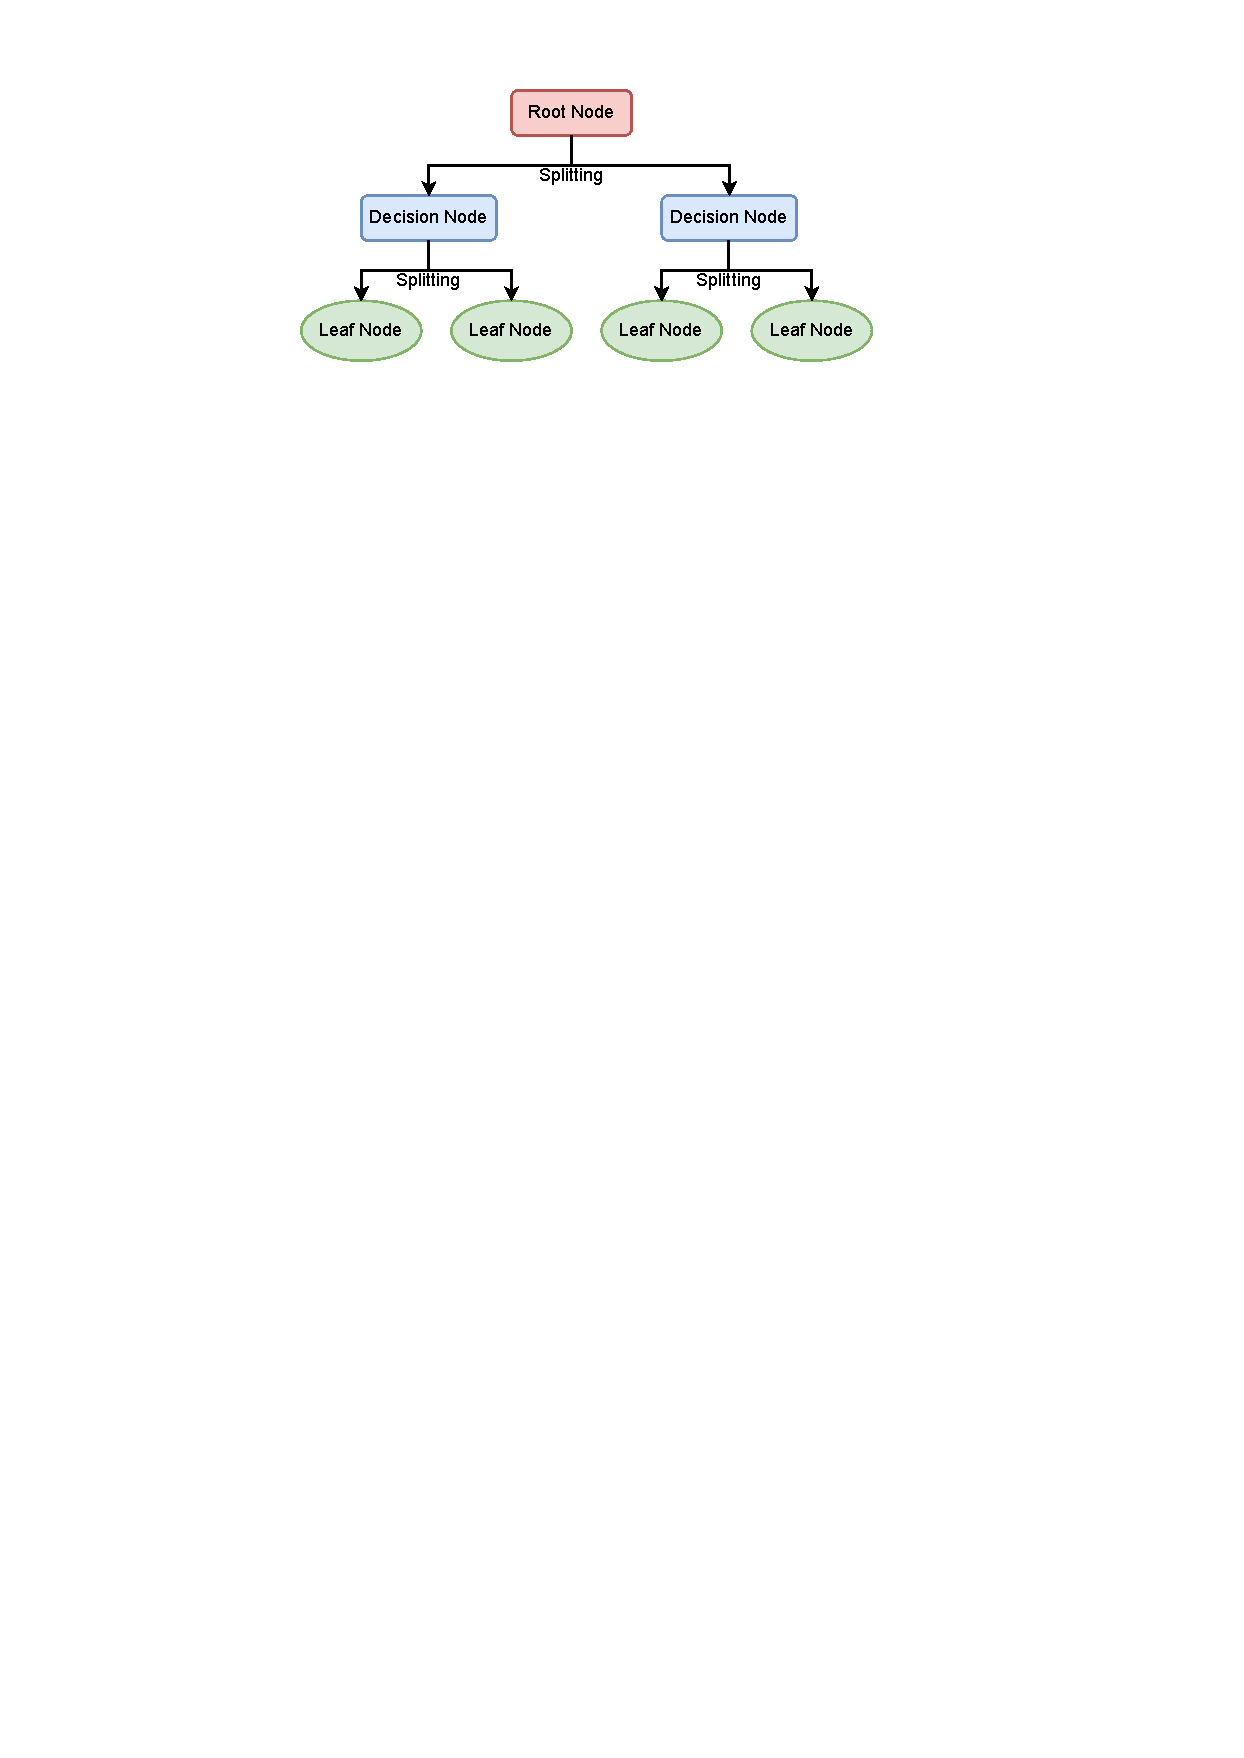
\includegraphics[width=0.6\textwidth]{figures/decision-tree.pdf}
    \caption{Decision tree structure}
    \label{fig_decision_tree}
\end{figure}

\subsection{Random forest}

Random forest \cite{598994} is an ensemble machine learning algorithm with many individual decision trees. Each tree in the random forest gives a prediction, of which the model's final prediction is the most voted class.

Extremely Randomized Trees (or Extra Trees) \cite{geurts2006extremely} is a type of ensemble learning technique that aggregates the results of multiple de-correlated decision trees to reach its final result. The fundamental difference between random forests and extra trees is selecting the cut points to create the decision trees. Extra Trees selects these cut-points comprehensively at random, while traditional decision tree-based algorithms (like Random Forest) select the optimal ones.

\subsection{K-Means clustering and silhouette analysis}
\label{subsec:silhouette}

K-means clustering \cite{Wu2012} is a linear clustering method widely used in data mining and machine learning that aims to partition data into several linearly separable homogeneous groups. It is an unsupervised learning method, meaning a training set is not required, making it more sensible for unlabelled data.

Silhouette analysis \cite{10.1007/978-3-319-62416-7_21} is an unsupervised method used for performance evaluation in machine learning for clustering algorithms such as k-means clustering, which examines the separation distance among resulting clusters and offers a visual means to evaluate parameters such as the number of clusters. The silhouette index in the plot effectively illustrates the proximity of each point within one cluster to points in neighboring clusters that fall within the range of [-1, 1].

Silhouette coefficients close to +1 imply that a sample is far from neighboring clusters, which means good separation. A value of 0 suggests the sample data is on or near the decision boundary between two adjacent clusters. In contrast, negative values imply the possibly wrong classification of a cluster. Furthermore, the thickness of the silhouette plot allows for the visualization of cluster sizes.

% Silhouette analysis can be used to evaluate the validity of the clustering results. It can be compared with the K-means cost function and the original silhouette to find the best way to automate the selection of the best clustering result from a set of K-means clusterings with different parameter configurations.

\section{Summary}
In this Section, we have delved into the intricacies of designing and implementing a real-time GPU monitoring and alerting system for large-scale distributed computing environments, focusing mainly on HPC clusters. By leveraging monitoring techniques, database technologies, and event stream management platforms, we aimed to address the need for efficient resource utilization and performance monitoring in these complex computing infrastructures.

The exploration began with an overview of Slurm, emphasizing its role in resource allocation, job scheduling, and management.

Subsequently, we provided insights into the architecture and specifications of three HPC systems at the CSC-IT Center for Science: Puhti, Mahti, and LUMI. These systems represent state-of-the-art computing clusters with diverse GPU configurations, highlighting the need for a flexible and scalable monitoring solution to accommodate varying hardware architectures.

We then delved into monitoring systems, exploring essential techniques and tools such as /proc, Cgroups, NVML, and ROCm-SMI for capturing resource utilization metrics at both the CPU and GPU levels. Additionally, we discussed the significance of time-series databases like TimescaleDB and related techniques such as triggers, LISTEN \& NOTIFY, and continuous aggregates in efficiently storing and querying monitoring data, enabling real-time analysis and visualization.

% Event stream management platforms such as MapReduce, Apache Spark, Apache Flink, and Apache Kafka/Pulsar were also examined, offering insights into their capabilities and ideal use cases for real-time data processing and analytics.

Finally, we explored various alert algorithms, including descriptive statistics, K-means clustering, silhouette analysis, decision trees, and random forests, as potential methods for identifying patterns or anomalies necessary to catch attention.

\clearpage
%!TEX root = ../Thesis.tex
\chapter{Methods}
\label{chap:methods}
Implementing real-time GPU resource monitoring and alerting involves systematically integrating various components. This chapter provides detailed insight into how we construct such a system, including the architecture, design, and implementation, covering key elements such as the monitoring system, alert service, and associated algorithms.

\section{Research process}
This section outlines the approach to achieving the thesis objectives, including designing, implementing, and evaluating the monitoring system and alert service for GPU resource utilization on HPC clusters.

\begin{enumerate}
    \item \textbf{Requirement Analysis}: We begin with a thorough analysis of the monitoring system and alert service requirements. This involves understanding the needs of HPC administrators and users and identifying key metrics and performance indicators for assessing GPU resource utilization and job efficiency.
    \item \textbf{System Design and Architecture}: The system design and architecture are developed based on the identified requirements. This phase involves defining the components of the monitoring system, including data collection mechanisms, storage infrastructure, and alert generation algorithms. Special attention is given to ensuring scalability, reliability, and compatibility with existing HPC cluster environments.
    \item \textbf{Implementation and Deployment}: With the system architecture finalized, the implementation phase commences. This involves developing the necessary software components for data collection, processing, and alert generation and integrating the monitoring system with the HPC cluster infrastructure. The deployment process includes configuration, testing, and validation to ensure the system operates effectively in a production environment.
    \item \textbf{Data Collection and Analysis}: Once deployed, the monitoring system collects real-time data on GPU usage and job performance. This data is then analyzed to identify patterns of inefficient resource utilization and inform the development of alert generation algorithms. Statistical analysis and machine learning techniques can be employed to extract insights from the collected data and optimize the performance of the alert service.
    \item \textbf{Evaluation and Validation}: The effectiveness and reliability of the monitoring system and alert service are evaluated through comprehensive testing and validation. This includes assessing the accuracy of alert notifications, evaluating the system's responsiveness to dynamic workload conditions, and validating the impact of the alert service on improving GPU resource utilization and job efficiency.
    \item \textbf{Feedback and Iterative Improvement}: Feedback from HPC administrators and users is solicited to identify areas for improvement and refinement. This feedback is incorporated into iterative cycles of system enhancement, enabling continuous improvement of the monitoring system and alert service over time.
    \item \textbf{Documentation and Knowledge Transfer}: Finally, comprehensive documentation is prepared to facilitate knowledge transfer and ensure the sustainability of the implemented solution. This includes user manuals, technical specifications, and best practice guides to support HPC administrators in effectively utilizing the monitoring system and alert service.
\end{enumerate}

Through this systematic methodology, the thesis aims to deliver a robust and effective solution for monitoring and alerting GPU resource utilization on HPC clusters, ultimately contributing to optimizing job scheduling, resource allocation, and overall system efficiency in GPU-accelerated computing environments.

\section{Monitoring system}
One of the issues faced by the users of HPC resources is that it is hard for them to see how well they are using the resources. This is an even bigger issue with the GPU nodes, where users often request GPUs without actually using them, or they may run jobs on the GPUs without putting any significant load.

Our monitoring system at the job level aims to improve observability and enable HPC system admins to find out these situations. It consists of several components with various roles that collect, process, store, and preset different metrics about jobs that are run in HPC systems:

\begin{itemize}
    \item \textbf{Monitoring Server}: Runs on all compute nodes and polls the performance metrics of jobs.
    \item \textbf{Monitoring Client}: Used by the Slurm prolog and epilog script to initiate the job collection.
    \item \textbf{TimescaleDB}: PostgreSQL database with an optimized extension for storing the time-series data and used to store job metrics and metadata.
    \item \textbf{Timescale Ingest}: Receives the metrics data from all monitoring servers and stores them into the TimescaleDB.
    \item \textbf{Timescale Reader}: Backend API loads data from TimescaleDB, enabling frontend UI or command line interface to render job statistics.
    \item \textbf{Timescale Chart}: Web interface to render user usage graphs.
    \item \textbf{Seff}: Command line interface to render user usage tables.
    \item \textbf{Lmod}: Environment module system used at CSC, and we configured the module load hook to send a notification to the monitoring server every time a module is loaded in the hope that we can better use this information to help debug the job as well as do classification on those jobs in the future.
\end{itemize}

% The monitoring system also collects status data and sends them to CSC's centralized logging system, Koivu.

Communication between different components during the lifetime of a job is presented in Figure \ref{fig_monitoring}. This section will then give a detailed description of the monitoring system design and how they work together.

\begin{figure}[H]
    \centering
    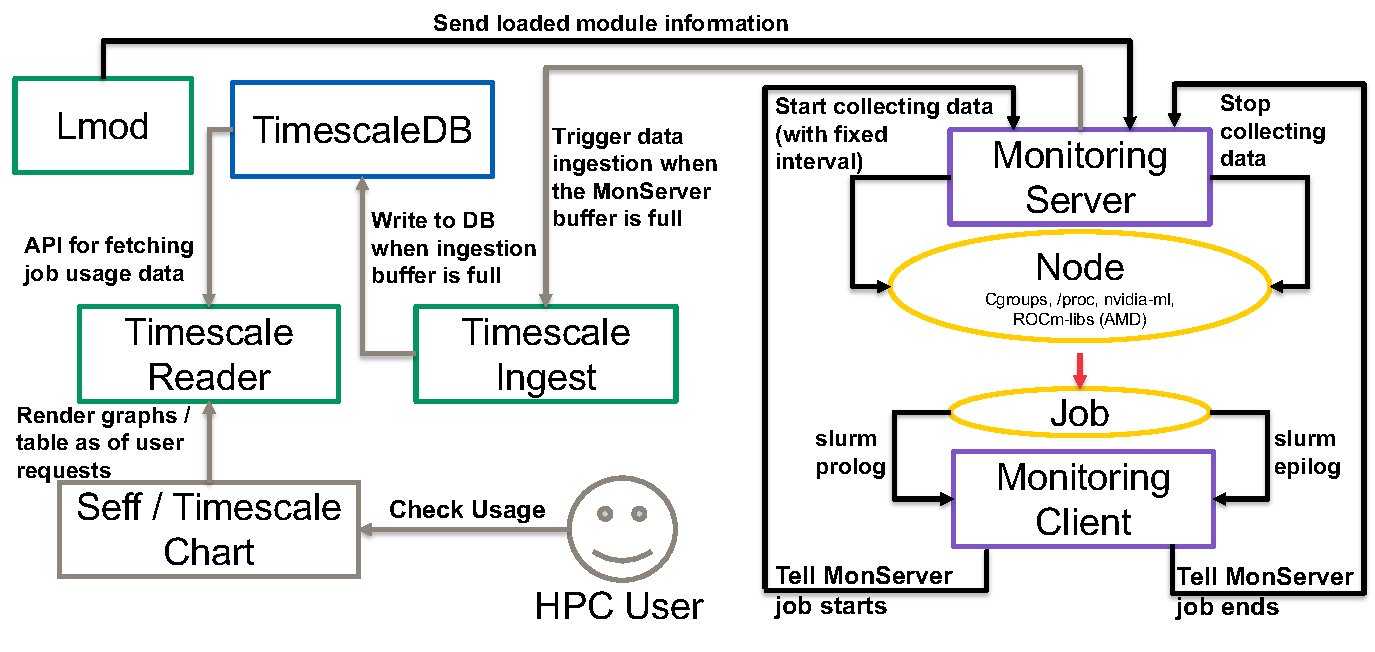
\includegraphics[width=1\textwidth]{figures/monitoring.pdf}
    \caption{Monitoring system structure}
    \label{fig_monitoring}
\end{figure}

\subsection{Monitoring Daemon}

Monitoring Daemon is written in C++ and consists of MonClient and MonServer. MonClient and MonServer are utilities that run on each compute node. They collect the job metadata and metrics and send them out from the node.

MonClient is a CLI utility that passes information about the job start and end to the MonServer process via UDP. MonClient commands are run in prolog and epilog scripts of jobs and tasks in Slurm.

MonServer runs continuously in the background of the compute nodes. It gets information about the job, such as hardware specifications, job ID, and step ID, from the client, collects the metrics of each job accordingly, and sends them to the Timescale Ingest server once the local buffer is complete so we can monitor how the actual hardware resources are used. The metrics that MonServer collects are as follows:

\begin{itemize}
    \item \textbf{CPU usage}: Reads the CPU metrics from \texttt{/proc} for the cores assigned to the job. Since the number of CPU cores can be too large to analyze individual jobs, we can also use the aggregated result of the assigned cores per node.
    \item \textbf{Memory usage per job}: Gets the total memory usage from Cgroups for the job per node. This requires that Slurm is set up to use the Cgroups plugin.
    \item \textbf{Memory usage per process}: Uses the \texttt{ps} command line utility to get the memory usage of processes for a job. \texttt{ps} needs the job step information from prolog and epilog scripts passed by MonClient to get the process ID information.
    \item \textbf{GPU usage}: Reads GPU load, memory, power, temperature, and energy information from Nvidia Management Library / ROCm-SMI for the GPUs assigned to the job.
\end{itemize}

We have intentional delays in collecting the monitoring data to filter out the IO loading period caused by dataset loading and environment initialization so that monitoring can genuinely reflect the use of GPU. Also, those jobs only last for a very short time, so we only collect from those jobs with a meaningful length of data to analyze and reduce the burden of the database and maintain the stability of the whole monitoring infrastructure. Data sent to the Timescale Ingest will be tagged with the job ID, the username, and the step ID if it is for memory usage per process.

We also support dropping those jobs from the collection loop that have exceeded the maximum possible end time configured by the partition or after two weeks in case the job is killed accidentally and the Slurm epilog does not run.


\subsection{Timescale Ingest}

Timescale Ingest offers API for data ingestion through HTTP or UDP. We use PBKDF2-HMAC-SHA256 with AES-GCM to do symmetric encryption on the monitoring data. The server is configured to handle incoming data according to the specified protocol. A UDP server is spun up in a separate thread (goroutine in Golang) if UDP is chosen. If HTTP is selected, the server sets up a route to handle incoming POST requests to the \textbf{/write} API endpoint. The transmitted data format follows the InfluxDB line protocol \cite{influxlineprotocol}.

We have an ingestion buffer to store the data temporarily in memory. Whenever we receive the data, we parse it into an instance of Go's structs. When the buffer is full or after a timeout, we sort the buffer by timestamp, convert them into SQL insert statements, and execute them together. This allows us to reduce the database's write load in batches.

Timescale Ingest implements the graceful shutdown, where a Goroutine uses a channel to wait for an interrupt signal (SIGINT or SIGTERM). Once the interrupt signal is received, the server initiates a graceful shutdown process, which involves creating a context with a timeout of 5 seconds, during which the server attempts to finish handling any ongoing requests and stops receiving new updates. The server is forcibly shut down after the timeout or when all requests are completed. Once the server is shut down, any remaining tasks should be completed. This includes closing the database connection, sending all the data in the buffer, and logging appropriate messages.

In addition to the /write API endpoint as demonstrated above, the API design for the Timescale Ingest is as follows:

\begin{itemize}
    \item \textbf{/version}: Displaying the version information and build time. If the current commit is tagged, \texttt{git describe} starts from the tagged commit and counts how many commits are on top of that tag. It then generates a string in the format of \textit{<tag>-<number\_of\_commits>-<short\_commit\_hash>}, where the tag is the name of the closest annotated one reachable from the commit, the number of commits is the count between the tagged commit and the current commit. The short commit hash is the current commit, abbreviated commit hash (typically seven characters).
    \item \textbf{/status}: A JSON-encoded representation of the server's current status, including information about the metrics being ingested. The JSON output contains fields such as \textit{ok} to indicate whether the operation was successful, \textit{msg} to provide any additional messages if the service has any error, and \textit{status} to contain the JSON-encoded heartbeat information with the key as follows:
    \begin{itemize}
        \item \textbf{BufferSize}: The number of metric items currently stored in the buffer.
        \item \textbf{BufferLimit}: The maximum number of metric items allowed in the buffer.
        % \item \textbf{Columns}: A mapping of column names to their respective data types in the data source schema.
        \item \textbf{CommitCount}: The count of commits made to the database.
        \item \textbf{ReceiveCount}: The count of metric items received by the server.
        \item \textbf{NextCommitTime}: The next time scheduled for committing to the database if the buffer is not full.
        \item \textbf{LastCommitDuration}: The duration it takes to commit the last buffer batch to the database.
        \item \textbf{CommitMetric}: The time taken per metric item to commit the last buffer batch to the database.
    \end{itemize}
    \item \textbf{/healthStatus}: A liveliness check for connection status between the timescale ingest and the database.
\end{itemize}

\subsection{TimescaleDB}
TimescaleDB, as the time-series database, introduces a relational aspect to monitoring. This component stores metrics in a structured manner, allowing for complex SQL queries and analysis. TimescaleDB accommodates the evolving nature of HPC workloads by enabling the retention of historical data. It also accelerates the query speed, which is essential for identifying trends and patterns over time.

Table \ref{tab:gpu_usage} shows how we define the database table for storing the GPU usage data at the job level collected by MonServer. This information gives us a basic idea of how well the job performs using GPUs.

\begin{table}[H]
    \centering
    \begin{tabular}{|l|l|l|}
        \hline
        Column & Type & Explanation \\
        \hline
        timestamp & TIMESTAMP & Time when the data is collected \\
        host & TEXT & Name of the host where data is from \\
        GPU & INT & ID of the GPU in the host machine \\
        username & TEXT & Name of the user that starts the job \\
        job & INT & ID of the job that uses the GPU \\
        load\_gpu & INT & Instantaneous GPU core load (\%, 0-100) \\
        load\_memory & INT & Instantaneous GPU memory load (\%, 0-100) \\
        used\_mem & BIGINT & Instantaneous GPU memory in use (Byte) \\
        total\_mem & BIGINT & Instantaneous GPU memory in total (Byte) \\
        power & INT & Instantaneous GPU power (mW for Nvidia, uW for AMD) \\
        temperature & INT & Instantaneous GPU temperature (°C for Nvidia, m°C for AMD) \\
        \hline
    \end{tabular}
    \caption{Table for storing GPU usage}
    \label{tab:gpu_usage}
\end{table}

Table \ref{tab:slurm_job_metadata} shows how we define the database table for storing the unstructured job information collected by MonClient. The JSON string in the metadata column represents the data structure containing information related to jobs, tasks, and allocated hardware information. Each JSON object corresponds to a specific event or action within Slurm indicated by the type, such as starting or stopping a job, task, or event. Every type follows a similar structure, containing fields such as \textit{method} (indicating the type of event), \textit{slurmInternalID} (job ID assigned by the Slurm workload manager), \textit{hostname} (name of the computing node), and \textit{gpu\_energy} (energy consumption data for GPUs), which contains the PCI Bus ID of each GPU as well as the energy counter when the event is triggered (in Millijoule, mJ). Here is a breakdown of each unique field of the types that happen in order during a job lifetime:

\begin{table}[H]
    \centering
    \begin{tabular}{|l|l|l|}
        \hline
        Column & Type & Explanation \\
        \hline
        timestamp & TIMESTAMP & Time when the data is collected \\
        host & TEXT & Name of the host where data is from \\
        job & INT & ID of the job that uses the GPU \\
        type & TEXT &  Type of the metadata (start/stop job/task, event) \\
        metadata & TEXT & Actual key-value data in JSON format \\
        \hline
    \end{tabular}
    \caption{Table for storing Slurm job metadata}
    \label{tab:slurm_job_metadata}
\end{table}

\begin{enumerate}
    \item \textbf{start-job} indicates initiating a new job. It includes details such as the user name (\textit{user}), user's ID (\textit{uid}), the group ID that the user belongs to (\textit{gid}), the partition that the job belongs to (\textit{partition}), and resource allocations, e.g., GPU and CPU id lists that get allocated to the job). Additionally, it includes the GPU energy counter of all the GPUs that belong to the node.
\begin{lstlisting}[language=JSON]
{
  "method":"start-job",
  "slurmInternalID":8934,
  "hostname":"g1101",
  "user":"dowjohn",
  "uid":100567,
  "gid":100567,
  "partition":"gputest",
  "gpu":"1",
  "cpu":"0-255",
  "gpu_energy":[
    {
      "pciBusId":"00000000:03:00.0",
      "energy":1260156826
    },
    {
      "pciBusId":"00000000:44:00.0",
      "energy":999985444
    },
    {
      "pciBusId":"00000000:84:00.0",
      "energy":793570107
    },
    {
      "pciBusId":"00000000:C4:00.0",
      "energy":708110133
    }
  ]
}
\end{lstlisting}

    \item \textbf{start-task}: indicates the start of a specific task within a job. It contains metadata such as the task's process ID, step ID (\textit{-1} indicates the batch step), node-local task ID for the process within a job (\textit{locaID}), number of processes in the job step or whole heterogeneous job step (\textit{stepTasks}) and loaded modules, which records the modules name as well as their versions separated by a colon. It also includes the GPU energy counter assigned to the job.

\begin{lstlisting}[language=JSON]
{
  "method":"start-task",
  "slurmInternalID":8934,
  "hostname":"g1101",
  "taskPID":44689,
  "stepID":-1,
  "locaID":0,
  "loadedModules":"gcc/11.2.0:openmpi/4.1.2:openblas/0.3.18-omp:csc-tools:StdEnv",
  "gpu_energy":[
    {
      "pciBusId":"00000000:44:00.0",
      "energy":999996492
    }
  ]
}
\end{lstlisting}

\begin{lstlisting}[language=JSON]
{
  "method":"start-task",
  "slurmInternalID":8934,
  "hostname":"g1101",
  "taskPID":45279,
  "stepID":0,
  "locaID":0,
  "stepTasks":1,
  "loadedModules":"csc-tools:StdEnv:gcc/9.4.0:tensorflow/2.12:openblas/0.3.18-omp:openmpi/4.1.2:cuda/11.5.0",
  "gpu_energy":[
    {
      "pciBusId":"00000000:44:00.0",
      "energy":1000040684
    }
  ]
}
\end{lstlisting}

    \item \textbf{event}: denotes the event that happens when the task is running. This can be that a new module is loaded in the job context.

\begin{lstlisting}[language=JSON]
{
  "method":"event",
  "slurmInternalID":8934,
  "stepID":0,
  "eventKind":"module-load",
  "eventField":"tensorflow/2.15"
}

\end{lstlisting}

    \item \textbf{stop-task}: denotes completing or terminating a task within a job. Like the start task, it includes metadata about the task and the energy consumption of GPUs allocated to the job during its execution.

\begin{lstlisting}[language=JSON]
{
  "method":"stop-task",
  "slurmInternalID":8934,
  "hostname":"g1101",
  "taskPID":44689,
  "stepID":0,
  "locaID":0,
  "stepTasks":1,
  "gpu_energy":[
    {
      "pciBusId":"00000000:44:00.0",
      "energy":1001166893
    }
  ]
}
\end{lstlisting}

\begin{lstlisting}[language=JSON]
{
  "method":"stop-task",
  "slurmInternalID":8934,
  "hostname":"g1101",
  "stepID":-1,
  "locaID":0,
  "gpu_energy":[
    {
      "pciBusId":"00000000:44:00.0",
      "energy":1001173148
    }
  ]
}
\end{lstlisting}

    \item \textbf{stop-job}: indicates the completion or termination of a job. It includes metadata about the job and the total energy consumption of all the GPUs inside the job running node during its execution.

\begin{lstlisting}[language=JSON]
{
  "method":"stop-job",
  "slurmInternalID":8934,
  "hostname":"g1101",
  "gpu_energy":[
    {
      "pciBusId":"00000000:03:00.0",
      "energy":1261452017
    },
    {
      "pciBusId":"00000000:44:00.0",
      "energy":1001180831
    },
    {
      "pciBusId":"00000000:84:00.0",
      "energy":794875873
    },
    {
      "pciBusId":"00000000:C4:00.0",
      "energy":709266506
    }
  ]
}
\end{lstlisting}

\end{enumerate}

We use TimescaleDB-specific features to improve query performance. We turn the metrics table into a hypertable with 6-hour chunking. We also create indexes on job IDs, hostnames, and GPU IDs, as those are the keys most commonly used for our SQL group queries. We compress data older than one day and drop data older than 6 months.

We define two triggers and corresponding notification functions in PL/pgSQL -- SQL Procedural language. These triggers are designed to automatically send notifications whenever new data is inserted into table \textit{slurm\_job\_metadata} and \textit{gpu\_usage}.

\begin{lstlisting}[language=SQL]
-- Notify of new job metadata
CREATE OR REPLACE FUNCTION notify_new_job_metadata_insertion()
  RETURNS trigger AS $notify_new_job_metadata_insertion$
BEGIN
  PERFORM pg_notify('job_updates', (NEW.host || '|' || NEW.job || '|' || NEW.type || '|' || NEW.metadata)::text);
  RETURN NEW;
END;
$notify_new_job_metadata_insertion$ LANGUAGE plpgsql;

CREATE TRIGGER job_metadata_insertion_notify_trigger
AFTER INSERT ON slurm_job_metadata
FOR EACH ROW EXECUTE FUNCTION notify_new_job_metadata_insertion();

-- Notify on new gpu_usage_aggregate data
CREATE OR REPLACE FUNCTION notify_new_gpu_usage_insertion()
  RETURNS trigger AS $notify_new_gpu_usage_insertion$
BEGIN
  PERFORM pg_notify('gpu_usage_insertion', (NEW.host || ',' || NEW.gpu || ',' || NEW.job || ',' || NEW.load_gpu || ',' || NEW.load_memory || ',' || NEW.used_mem || ',' || NEW.power || ',' || NEW.temperature)::text);
  RETURN NEW;
END;
$notify_new_gpu_usage_insertion$ LANGUAGE plpgsql;

CREATE TRIGGER gpu_usage_insertion_notify_trigger
AFTER INSERT ON gpu_usage
FOR EACH ROW EXECUTE FUNCTION notify_new_gpu_usage_insertion();
\end{lstlisting}


\begin{itemize}
    \item \textbf{notify\_new\_job\_metadata\_insertion()}: This function retrieves the newly inserted row and constructs a notification message using concatenation (\textit{||}). The message includes all the fields except the timestamp from the inserted row. Finally, the \textit{pg\_notify()} function is called to send a notification to a specific channel named \textit{job\_updates}.
    \item \textbf{job\_metadata\_insertion\_notify\_trigger}: This trigger fires after each insertion into the \textit{slurm\_job\_metadata} table. It is associated with the \\
    \textit{notify\_new\_job\_metadata\_insertion()} function, causing the function to execute automatically whenever new data is inserted into the table.
    \item \textbf{notify\_new\_gpu\_usage\_insertion()}: Similar to the first function, it constructs a notification message using all the fields except the timestamp, username, and total\_mem from the inserted row. It then sends a notification to the \textit{gpu\_usage\_insertion} channel.
    \item \textbf{gpu\_usage\_insertion\_notify\_trigger}: This trigger fires after each insertion into the \textit{gpu\_usage} table and is associated with the \textit{notify\_new\_gpu\_usage\_insertion()} function, triggering it automatically upon insertion of new data.
\end{itemize}

These triggers and notification functions facilitate real-time communication within the database system. They enable other parts of the system to be notified instantly whenever new job metadata or GPU usage data is inserted, allowing for timely updates and actions based on the newly inserted data.

\subsection{Timescale Reader}
The Timescale Reader component facilitates the retrieval of metrics from TimescaleDB for analysis and reporting. It provides a RESTful API for building other elements that support administrators in gaining insights into historical resource utilization, aiding in capacity planning, performance optimization, and trend analysis. It also enables the integration of other components to show statistics to users via GUI or CLI. The Timescale Reader complements the real-time monitoring capabilities, providing a comprehensive view of metrics across different time intervals.

We have a centralized web page that allows users to use the APIs provided by Timescale Reader to check job usage data, as shown in Figure \ref{fig_gpu-usage-history-dashboard}. Figure \ref{fig_gpu-usage-graph} shows one example of a graph rendered via Timescale Chart through Timescale Reader API data. It also has accessibility support to help viewers with vision deficiencies (e.g., color blindness or partial sight) more easily understand the data with patterns and gradients, as shown in Figure \ref{fig_gpu-usage-graph-accessibility}.

\begin{figure}[H]
    \centering
    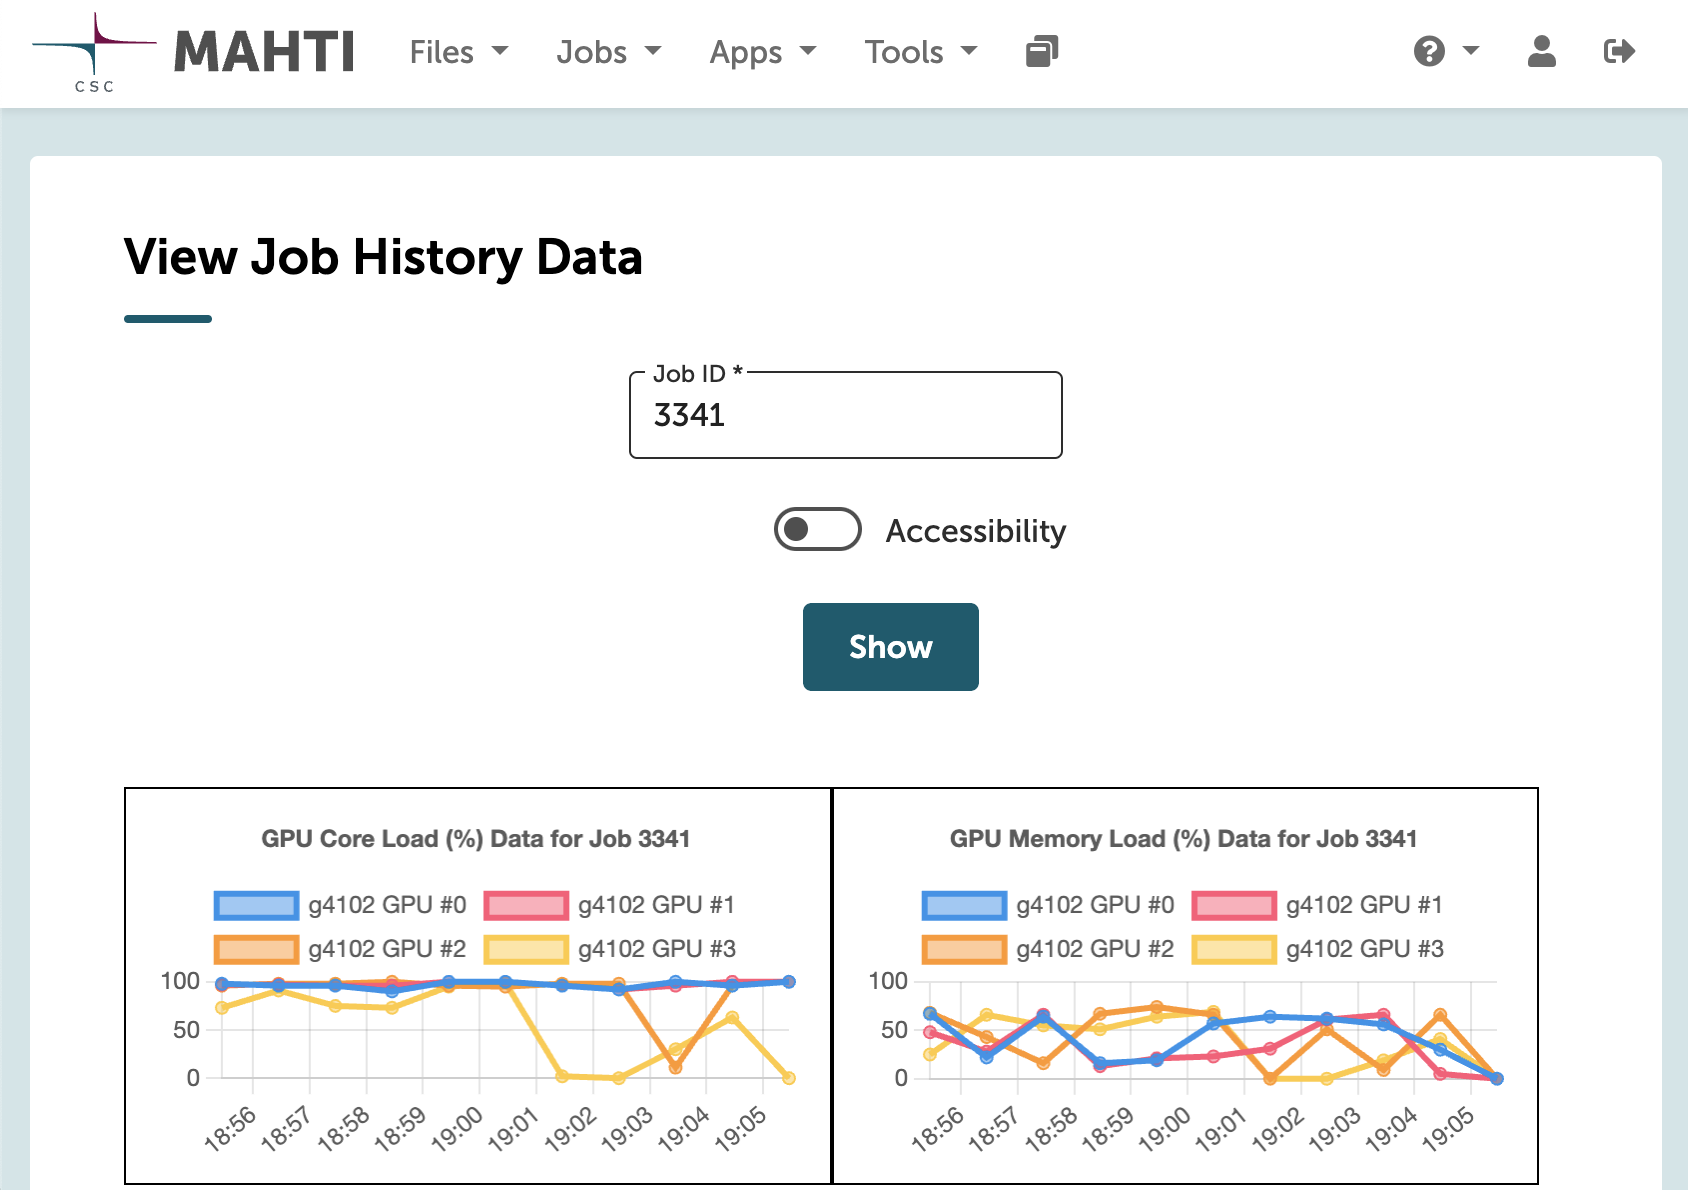
\includegraphics[width=1\textwidth]{figures/data-dashboard.png}
    \caption{GPU usage history checking dashboard}
    \label{fig_gpu-usage-history-dashboard}
\end{figure}

\begin{figure}[H]
    \centering
    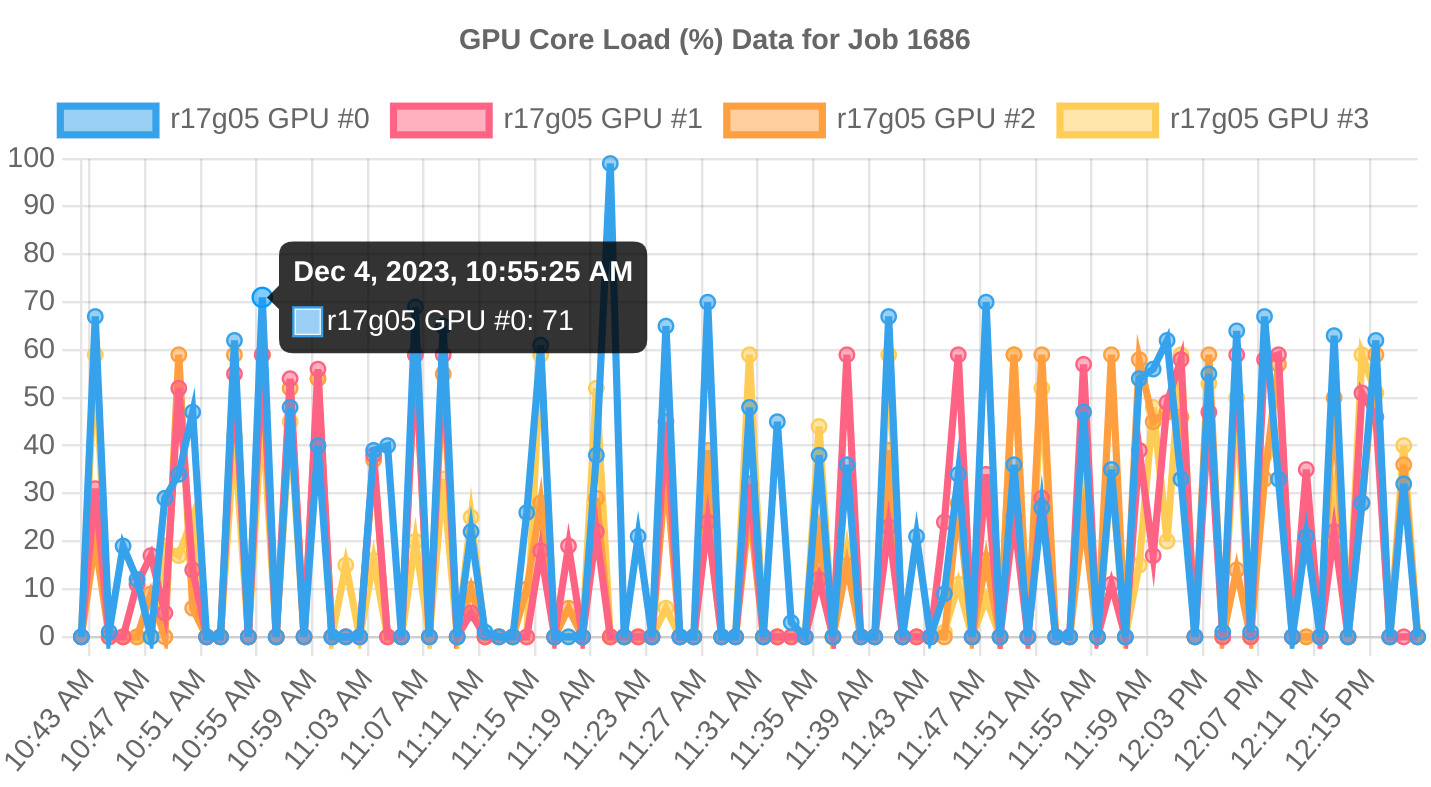
\includegraphics[width=1\textwidth]{figures/usage-graph.png}
    \caption{GPU usage history graph from Timescale Chart}
    \label{fig_gpu-usage-graph}
\end{figure}

\begin{figure}[H]
    \centering
    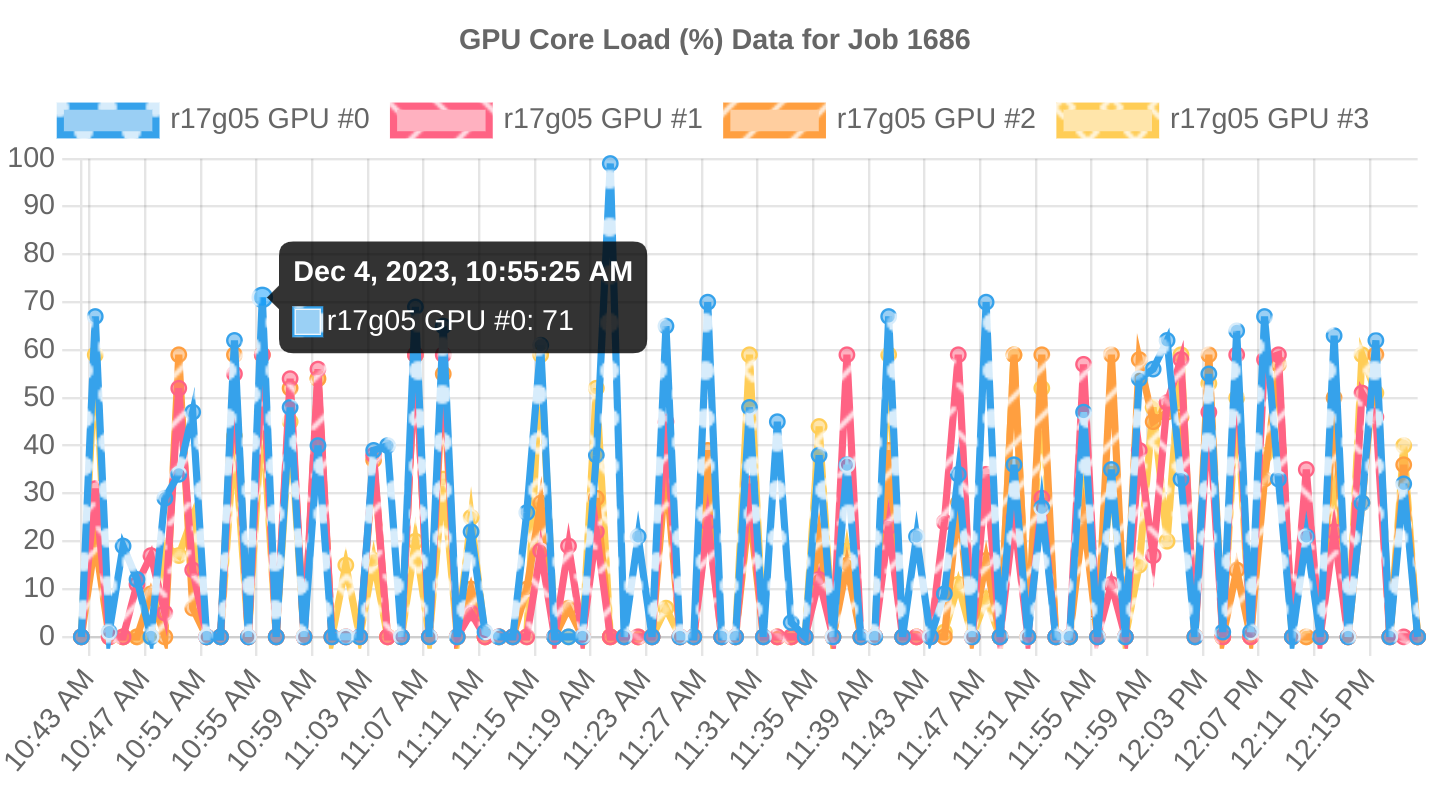
\includegraphics[width=1\textwidth]{figures/usage-accessibility-graph.png}
    \caption{GPU usage history graph from Timescale Chart with accessibility}
    \label{fig_gpu-usage-graph-accessibility}
\end{figure}

Below is an example showing the output of the \textit{seff} command. The GPU job efficiency section is printed via the Timescale Reader API. Here, we show the metrics related to the GPU, including the load, memory, and energy. Each entry shows the hostname, and the GPU ID that are related to the metrics, as well as the aggregated mean, standard deviation, and maximum value for the whole job history.

\begin{lstlisting}
$ seff 5465
Job ID: 5465
Cluster: mahti
User/Group: johndoe/pepr_johndoe
State: COMPLETED (exit code 0)
Nodes: 1
Cores per node: 16
CPU Utilized: 19-19:45:45
CPU Efficiency: 82.58% of 24-00:05:52 core-walltime
Job Wall-clock time: 1-12:00:22
Memory Utilized: 14.41 GB
Memory Efficiency: 22.51% of 64.00 GB
Job consumed 3600.61 CSC billing units based on the following used resources.
Billed project: project_1008888
Non-Interactive BUs: 3600.61
GPU BU: 7201.22
NVME BU: 38.89
GPU job efficiency:
-------------------------------------------------------------------
GPU load
    Hostname      GPU Id      Mean (%)    stdDev (%)       Max (%)
       g5101           0         86.21         18.69         99.00
       g5101           3         78.53         19.65         97.00
-------------------------------------------------------------------
GPU memory
    Hostname      GPU Id    Mean (GiB)  stdDev (GiB)     Max (GiB)
       g5101           0         22.64          0.00         22.64
       g5101           3         22.32          0.00         22.33
-------------------------------------------------------------------
GPU energy
    Hostname      GPU Id   Energy (Wh)
       g5101           0       8532.60
       g5101           3       8664.34
-------------------------------------------------------------------
\end{lstlisting}

To integrate with the existing authentication mechanism, Timescale Reader will check the \textit{From:} header in the HTTP request. The request can set that header's value \textit{*} to unlimited data access. Otherwise, the user name will be set, and access to the data of the jobs will be limited to those jobs started by the user.

The API design for the Timescale Reader is as follows:

\begin{itemize}
    \item \textbf{/version}: Same as Timescale Ingest, it displays the version information and build time.
    \item \textbf{/status}: Liveness checking endpoint.
    \item \textbf{/chart}: Serving the static files for Timescale Chart JS web interface, available parameters can be referred from Table \ref{tab:chart_params}.
    \item \textbf{/getJobs}: Endpoint for listing all the available job IDs in the database with valid GPU monitoring data, meaning those jobs are long enough to collect the data.
    \item \textbf{/getData/:table/:jobid}: Fetching the raw (unaggregated) history data in JSON format to be rendered by Timescale Chart.
    \item \textbf{/getLoad/:metric/:resource/:jobid/:type}: Displaying aggregated result of the history monitoring data.
    \item \textbf{/getGPUEnergy/:jobid}: Displaying the GPU energy counter.
\end{itemize}


\begin{table}[H]
\centering
\caption{Timescale Chart parameter description}
\begin{tabular}{|l|p{10cm}|}
\hline
\textbf{Parameter} & \textbf{Description} \\ \hline
api & API endpoint to read data from, such as \texttt{http://localhost:8001/getData}. Default to be \texttt{/getData} at the same site. \\ \hline
domain & Database table name to read from, such as \texttt{gpu\_usage}. \\ \hline
job & Job ID to be displayed. \\ \hline
title & Title of the chart. \\ \hline
group & Grouping of the data for different domain datasets, such as \texttt{core} (for \texttt{CPU usage}), \texttt{gpu} (for \texttt{GPU usage}), \texttt{pid} (for \texttt{Memory usage by PID}). \\ \hline
metric & Column name of the data to be displayed in the specific table. \\ \hline
name & Name of the group that will be displayed. \\ \hline
divide & Value to divide the data with. \\ \hline
mode & Chart zoom and pan mode, available values are \texttt{xy}, \texttt{x}, \texttt{y}. The default is \texttt{x}, which means zoom only at the x-axis. \\ \hline
type & Chart graph type, default is \texttt{line} \\ \hline
\end{tabular}
\label{tab:chart_params}
\end{table}

The parameters we support for displaying the aggregated result of the history monitoring data, as well as the GPU energy counter, are as follows:

\begin{itemize}
    \item \textbf{display}: 1 for printing in human-readable format, 2 for printing a table (similar to human-readable format but separated by tabs), and any other values will be in JSON format organized by a list of values using the hostname as the top level and hardware ID as the second level.
    \item \textbf{unit}: Specify the unit of the value to be printed.
    \item \textbf{type}: Specify the name of the value.
    \item \textbf{metric}: Specify the metric of the value (average, minimum, maximum, standard deviation, etc.), support multiple metrics separated by \textit{,} (comma).
    \item \textbf{divide}: Divide the data value stored in the database by this specified number.
    \item \textbf{precision}: Specify the precision of the value to be printed. The default is 2. -1 for no rounding.
    \item \textbf{index}: Specify the device's index to get printed. The default is all devices.
    \item \textbf{hide\_device}: 1 for hiding the \texttt{[device]}, other values for printing the \texttt{[device]}.
\end{itemize}

The human-readable printing format is as follows. Note that \#[\text{index}] will only get printed when there is more than one.

\begin{equation*}
[\text{device}]~\#[\text{index}]~([\text{type}] \ [\text{metric}]):~[\text{value}] \ [\text{unit}]
\end{equation*}


\section{Alert algorithms}
The Alert algorithms component comprises predefined algorithms, that determine the conditions under which alerts are triggered. These algorithms consider various factors, including GPU utilization thresholds and temperature limits. The flexibility of the alert algorithms allows for customization --- based on the specific requirements of HPC clusters --- ensuring that alerts are triggered for conditions deemed critical by administrators.

Regarding the design of the alert algorithms for GPU usage: many high-performance computing applications have load-balancing issues regarding pipeline parallelism, and the data has highly fluctuated characteristics for multiple GPU jobs. Thus, alerting only according to average is neither reliable nor practical, as it may not be fixable easily by the user, so those can be non-critical. Machine learning models could be one way to address the data fluctuation issue by recognizing the data pattern.

Unsupervised machine learning, such as reinforcement learning, is hard to train and interpret. Deep learning algorithms are also very slow to run, so they might not fit our need for real-time job analysis. Most importantly, we cannot find a good reward function. The only way seems to be from human feedback.

For supervised machine learning, such as random forests that involve decision trees, although it can be much faster to run, all the data collected from the monitoring system is unlabeled. It is unrealistic for humans to label all those millions of data manually.

In the hope of doing labeling automatically, we also did the silhouette analysis of K-means clustering on the collected GPU monitoring data starting from December 2023 directly, as shown in Figure \ref{fig_silhouette_directly}, as well as features generated with statistical aggregation, as shown in Figure \ref{fig_silhouette_statistics}. Each color in the figure represents a cluster, the red vertical line denotes the average silhouette coefficient value across all clusters. More explanation of silhouette analysis can be found in Subsection \ref{subsec:silhouette}. The result shows that neither of the methods works well since most clusters have the majority proportion of negative coefficient value, and they cannot act as reasonable classifications. 

\begin{figure}[H]
    \centering
        \subfloat[n\_clusters = 2]{
        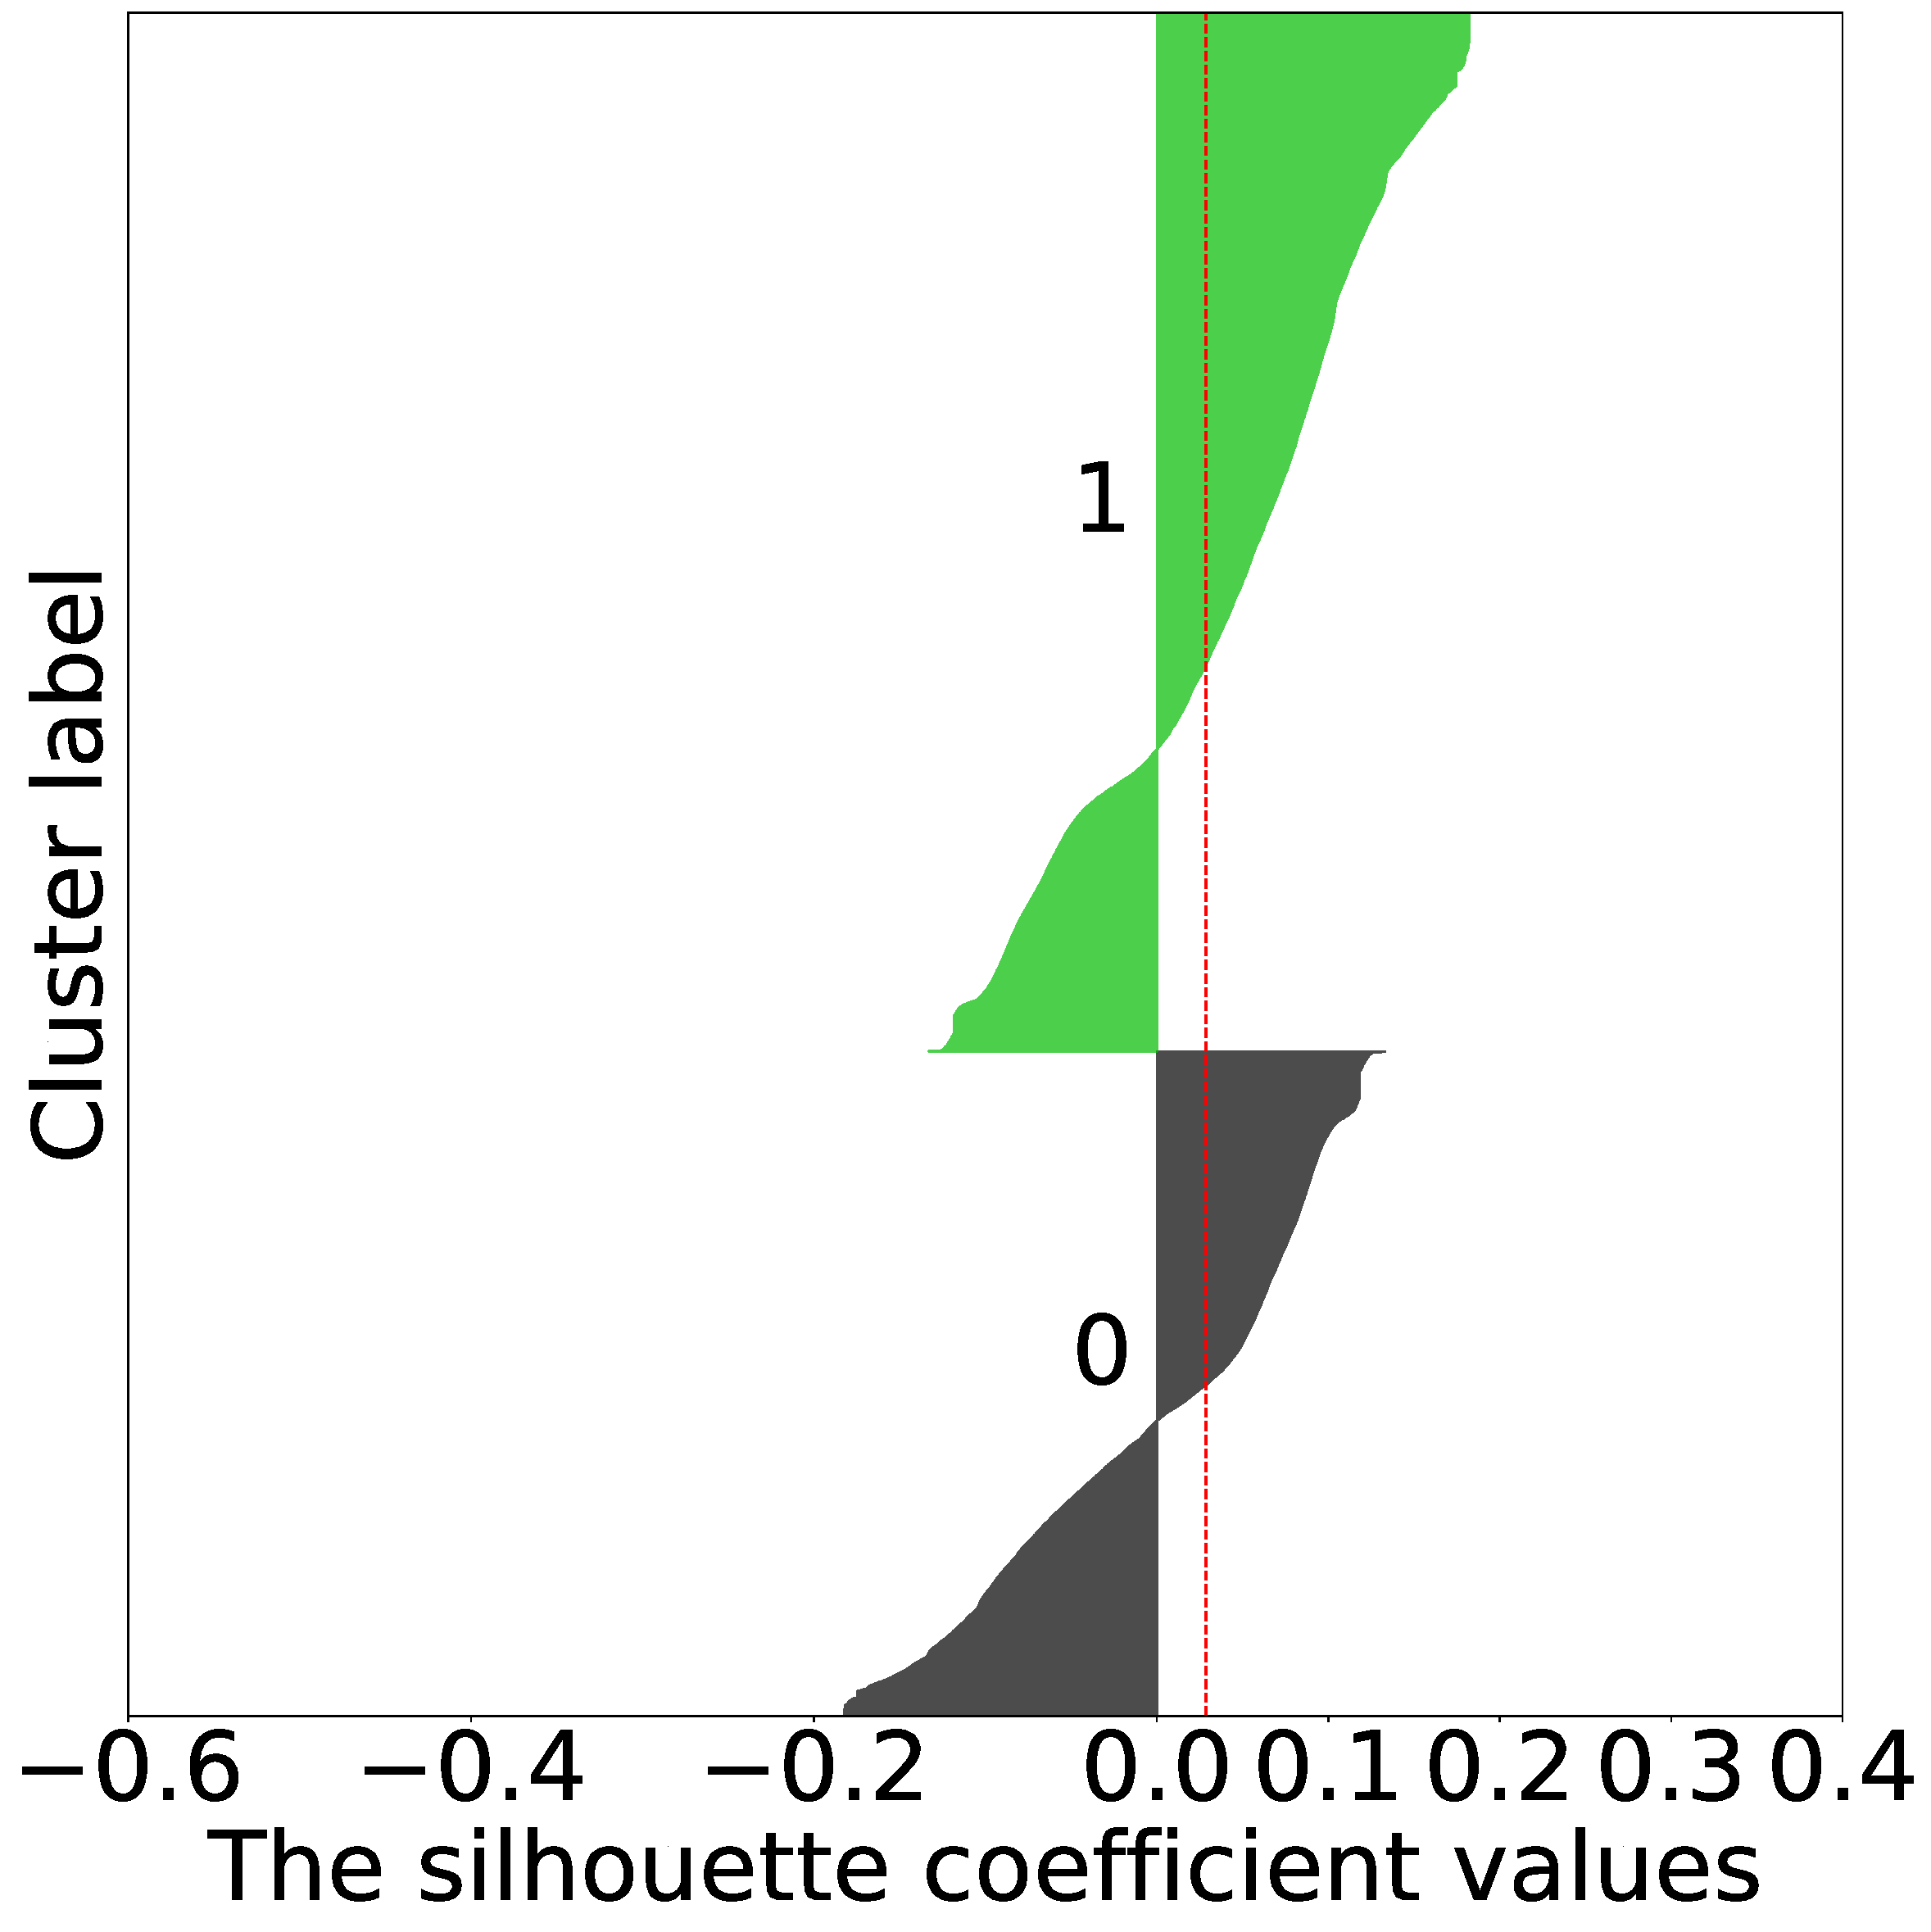
\includegraphics[width=0.33\textwidth]{figures/silhouette/silhouette_directly_2.pdf}
    }
        \subfloat[n\_clusters = 3]{
        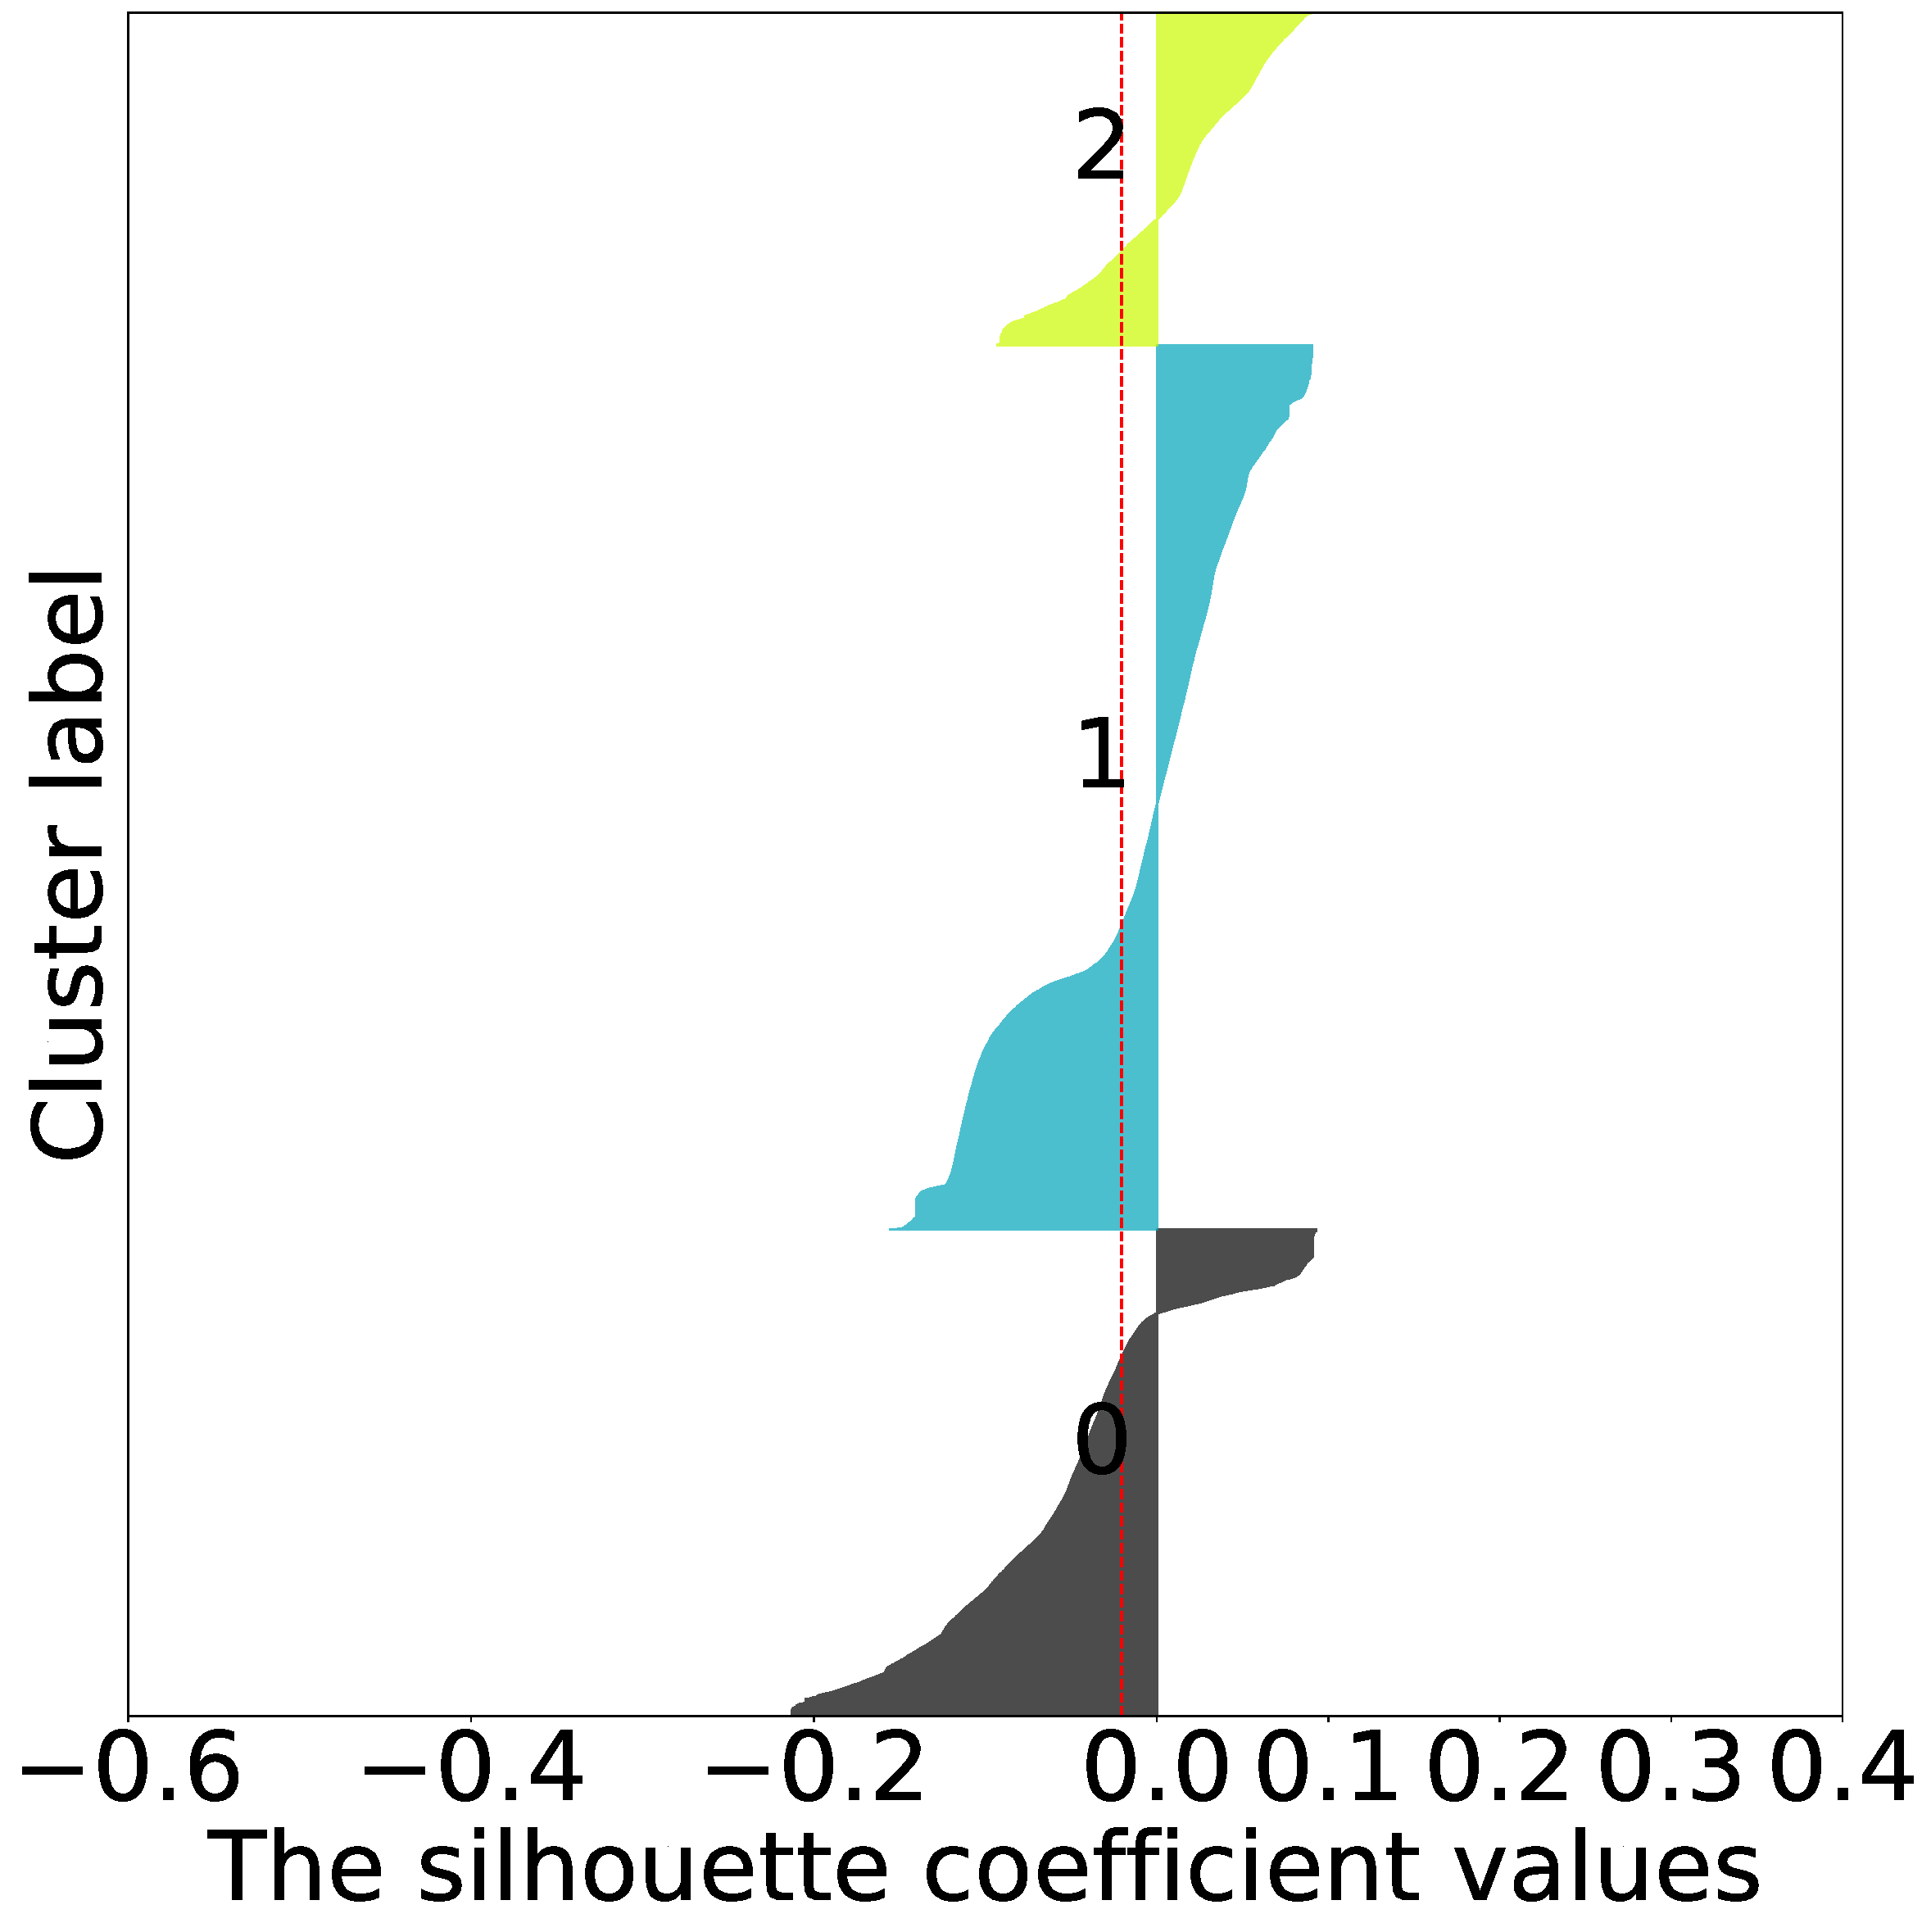
\includegraphics[width=0.33\textwidth]{figures/silhouette/silhouette_directly_3.pdf}
    }
        \subfloat[n\_clusters = 4]{
        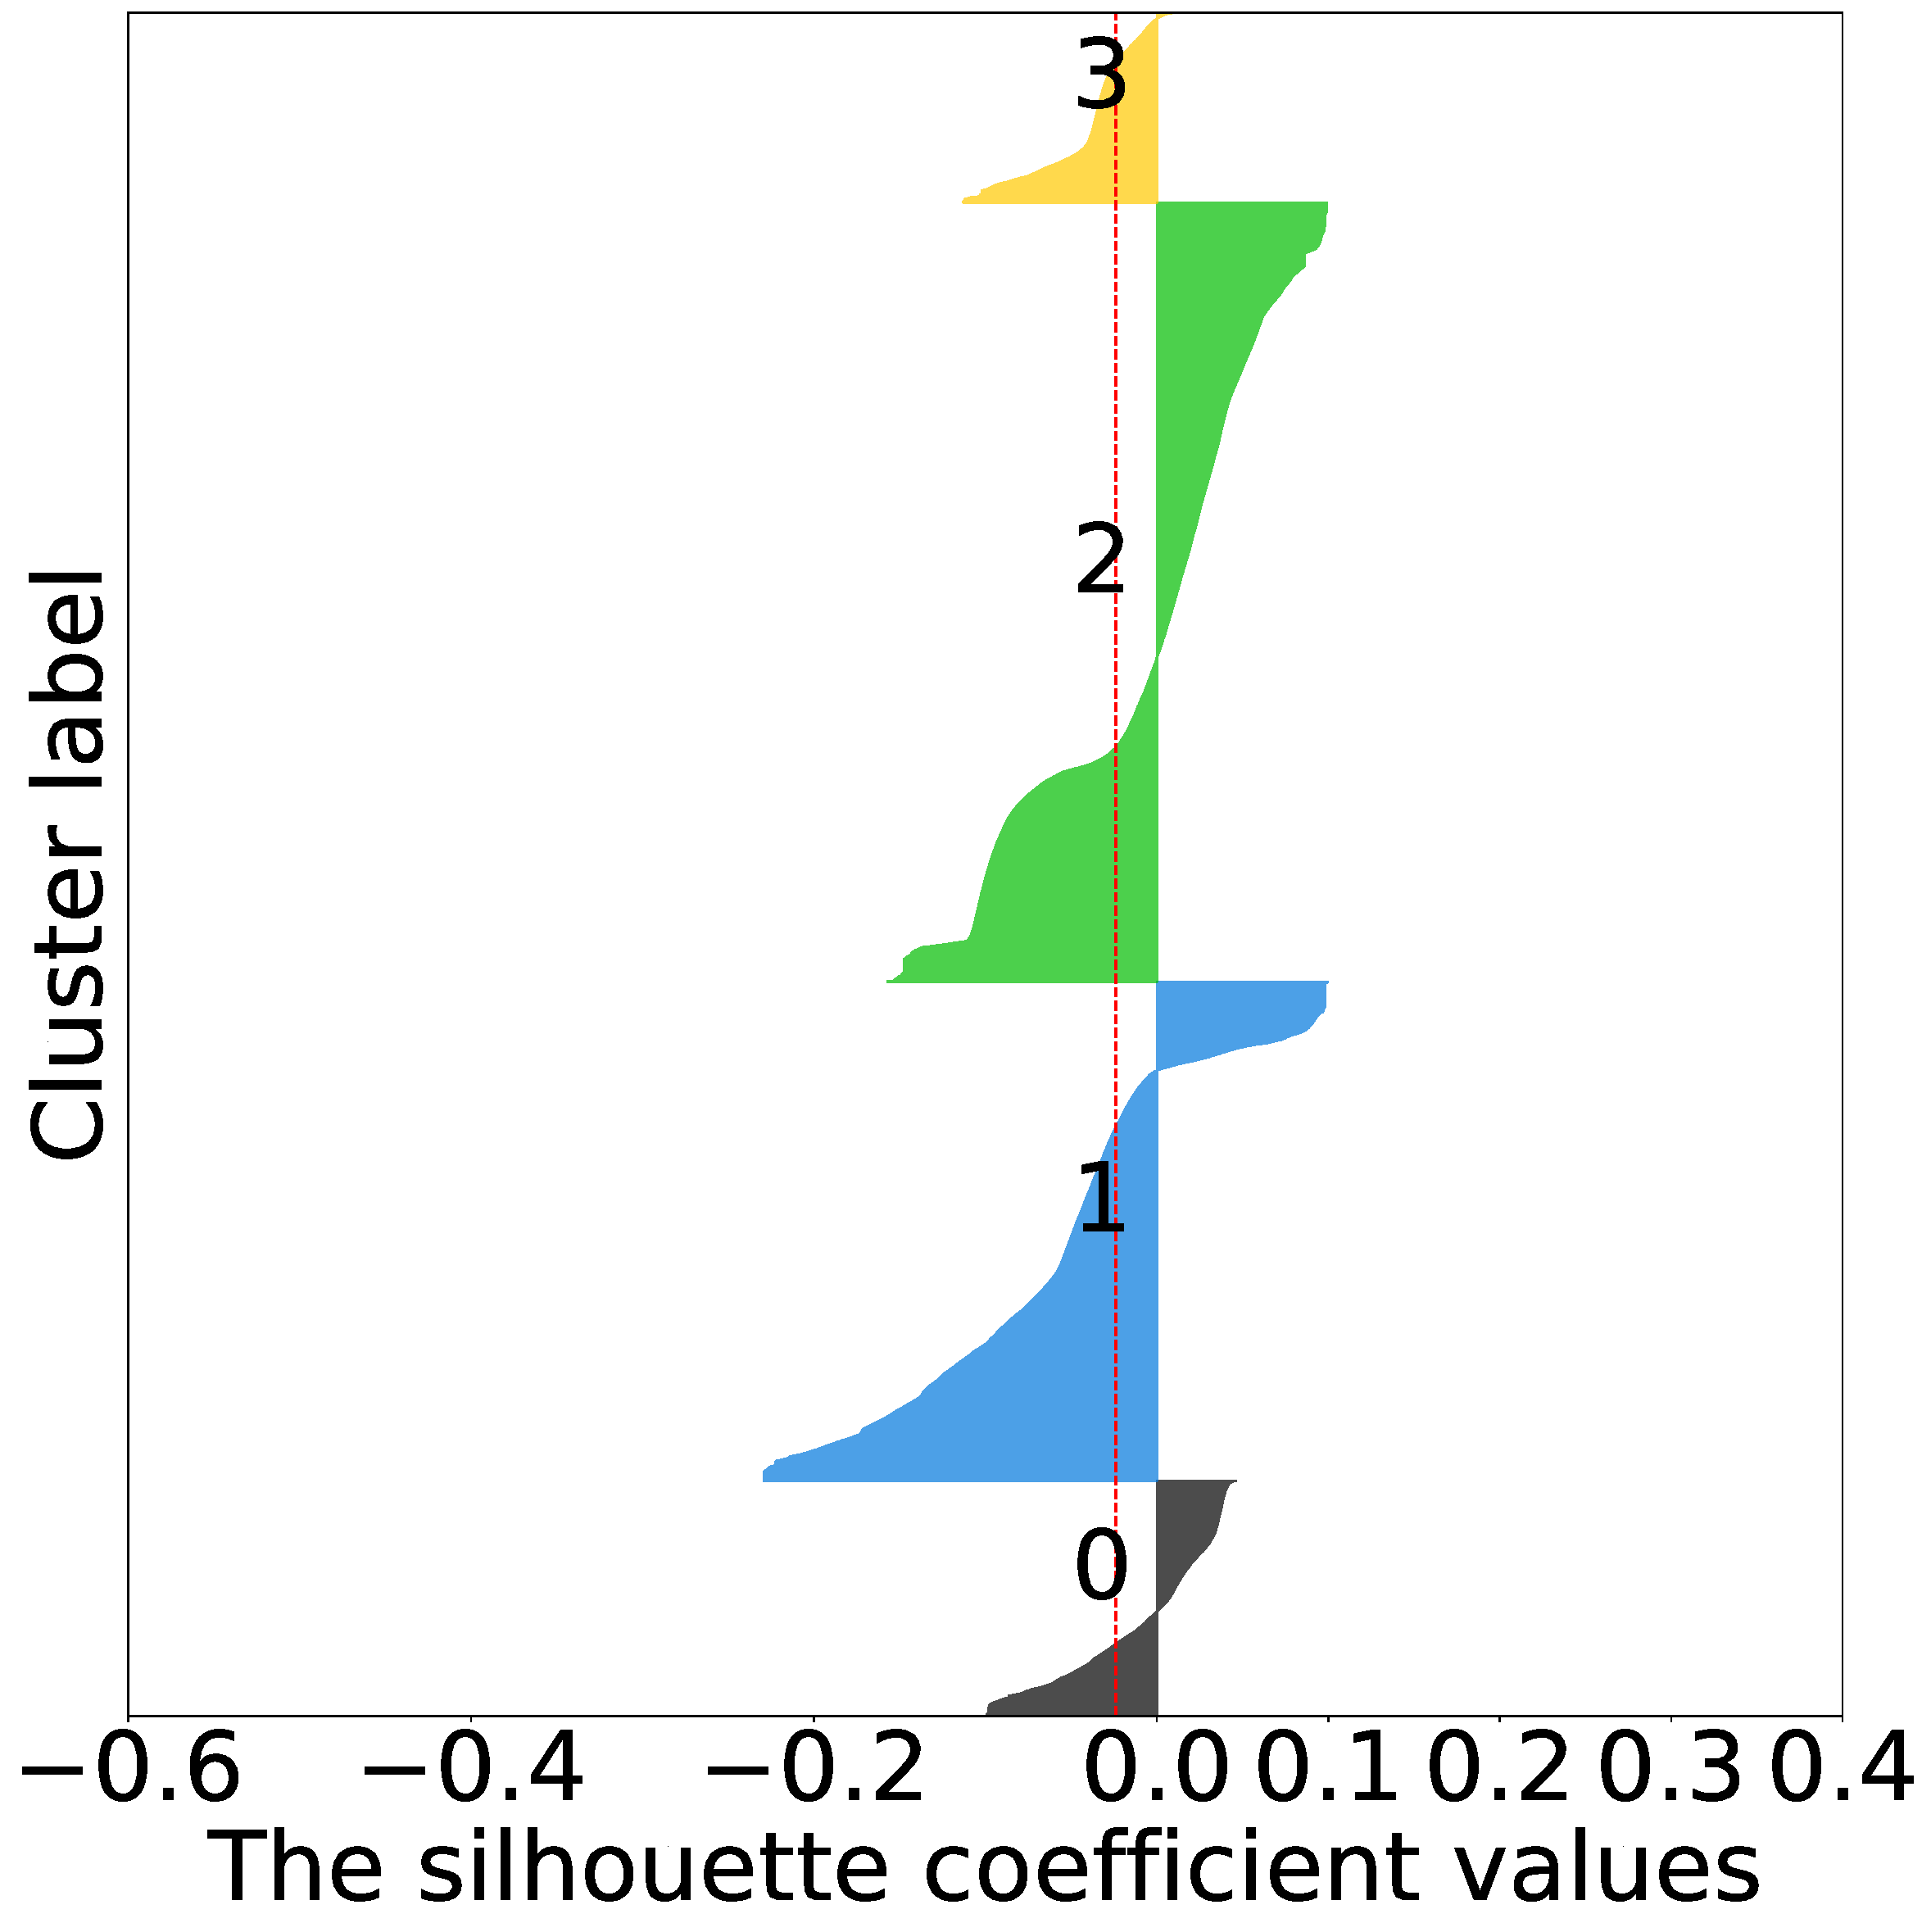
\includegraphics[width=0.33\textwidth]{figures/silhouette/silhouette_directly_4.pdf}
    }\\
        \subfloat[n\_clusters = 5]{
        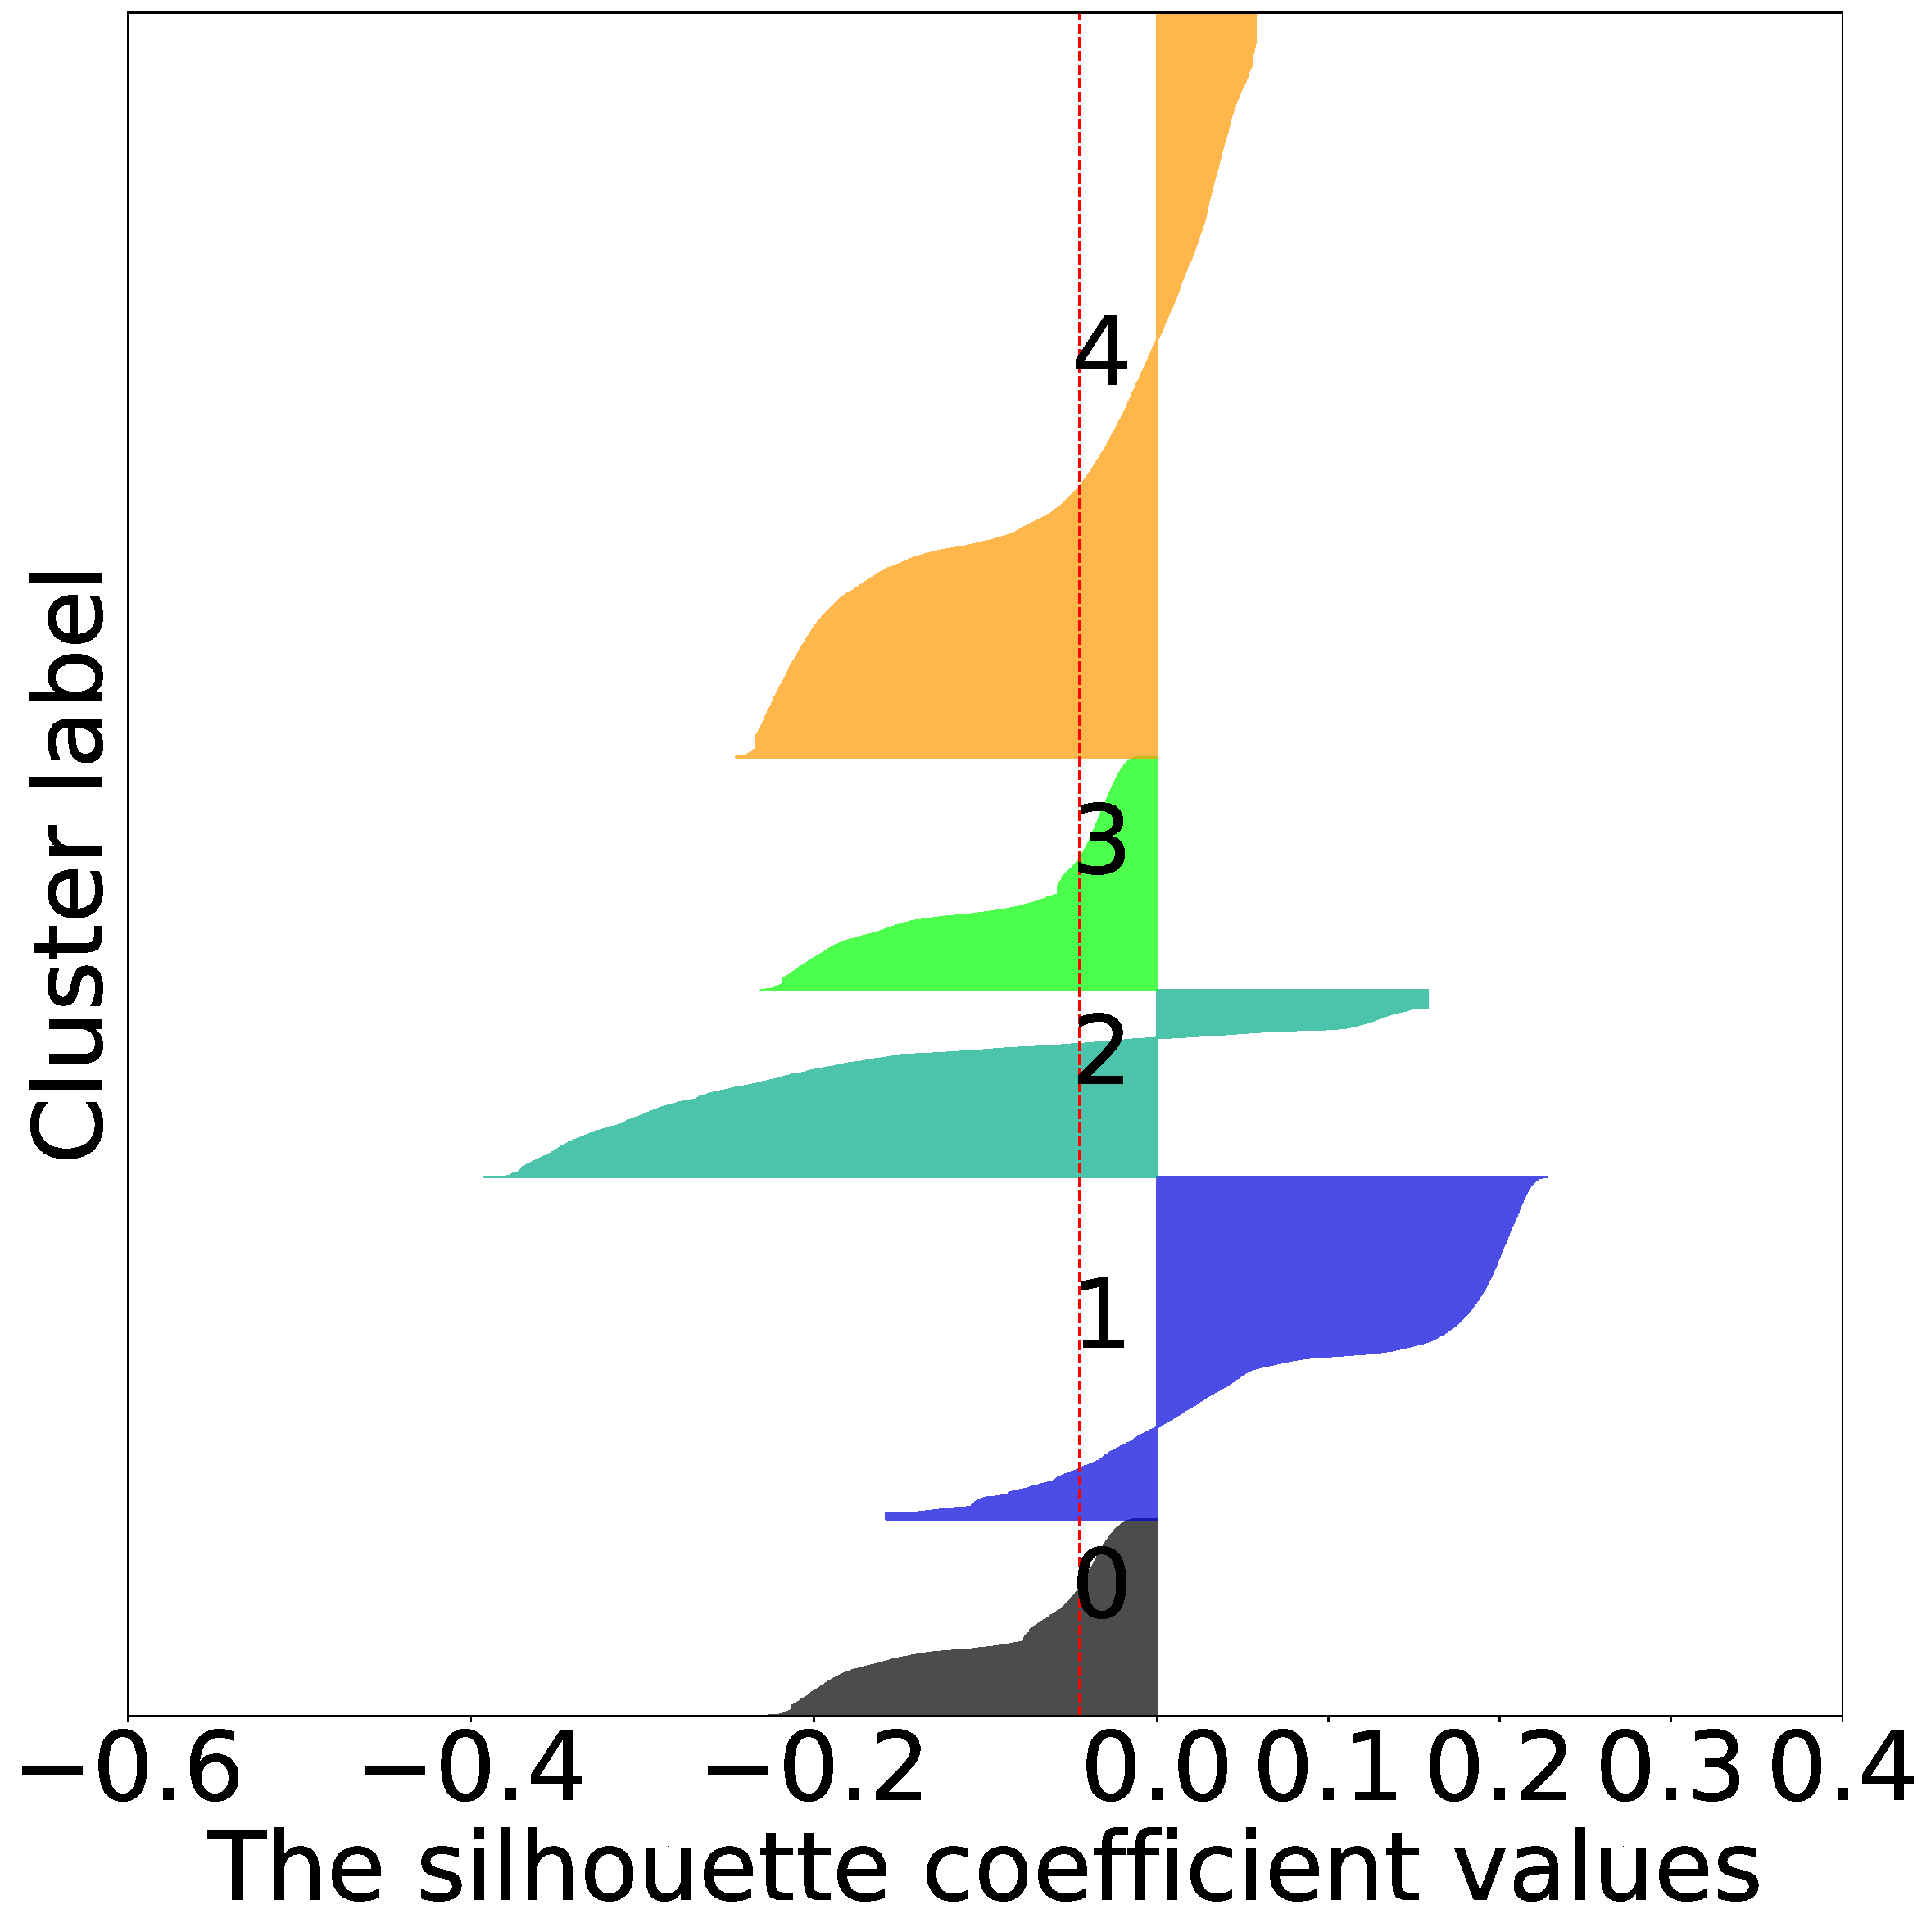
\includegraphics[width=0.33\textwidth]{figures/silhouette/silhouette_directly_5.pdf}
    }
        \subfloat[n\_clusters = 6]{
        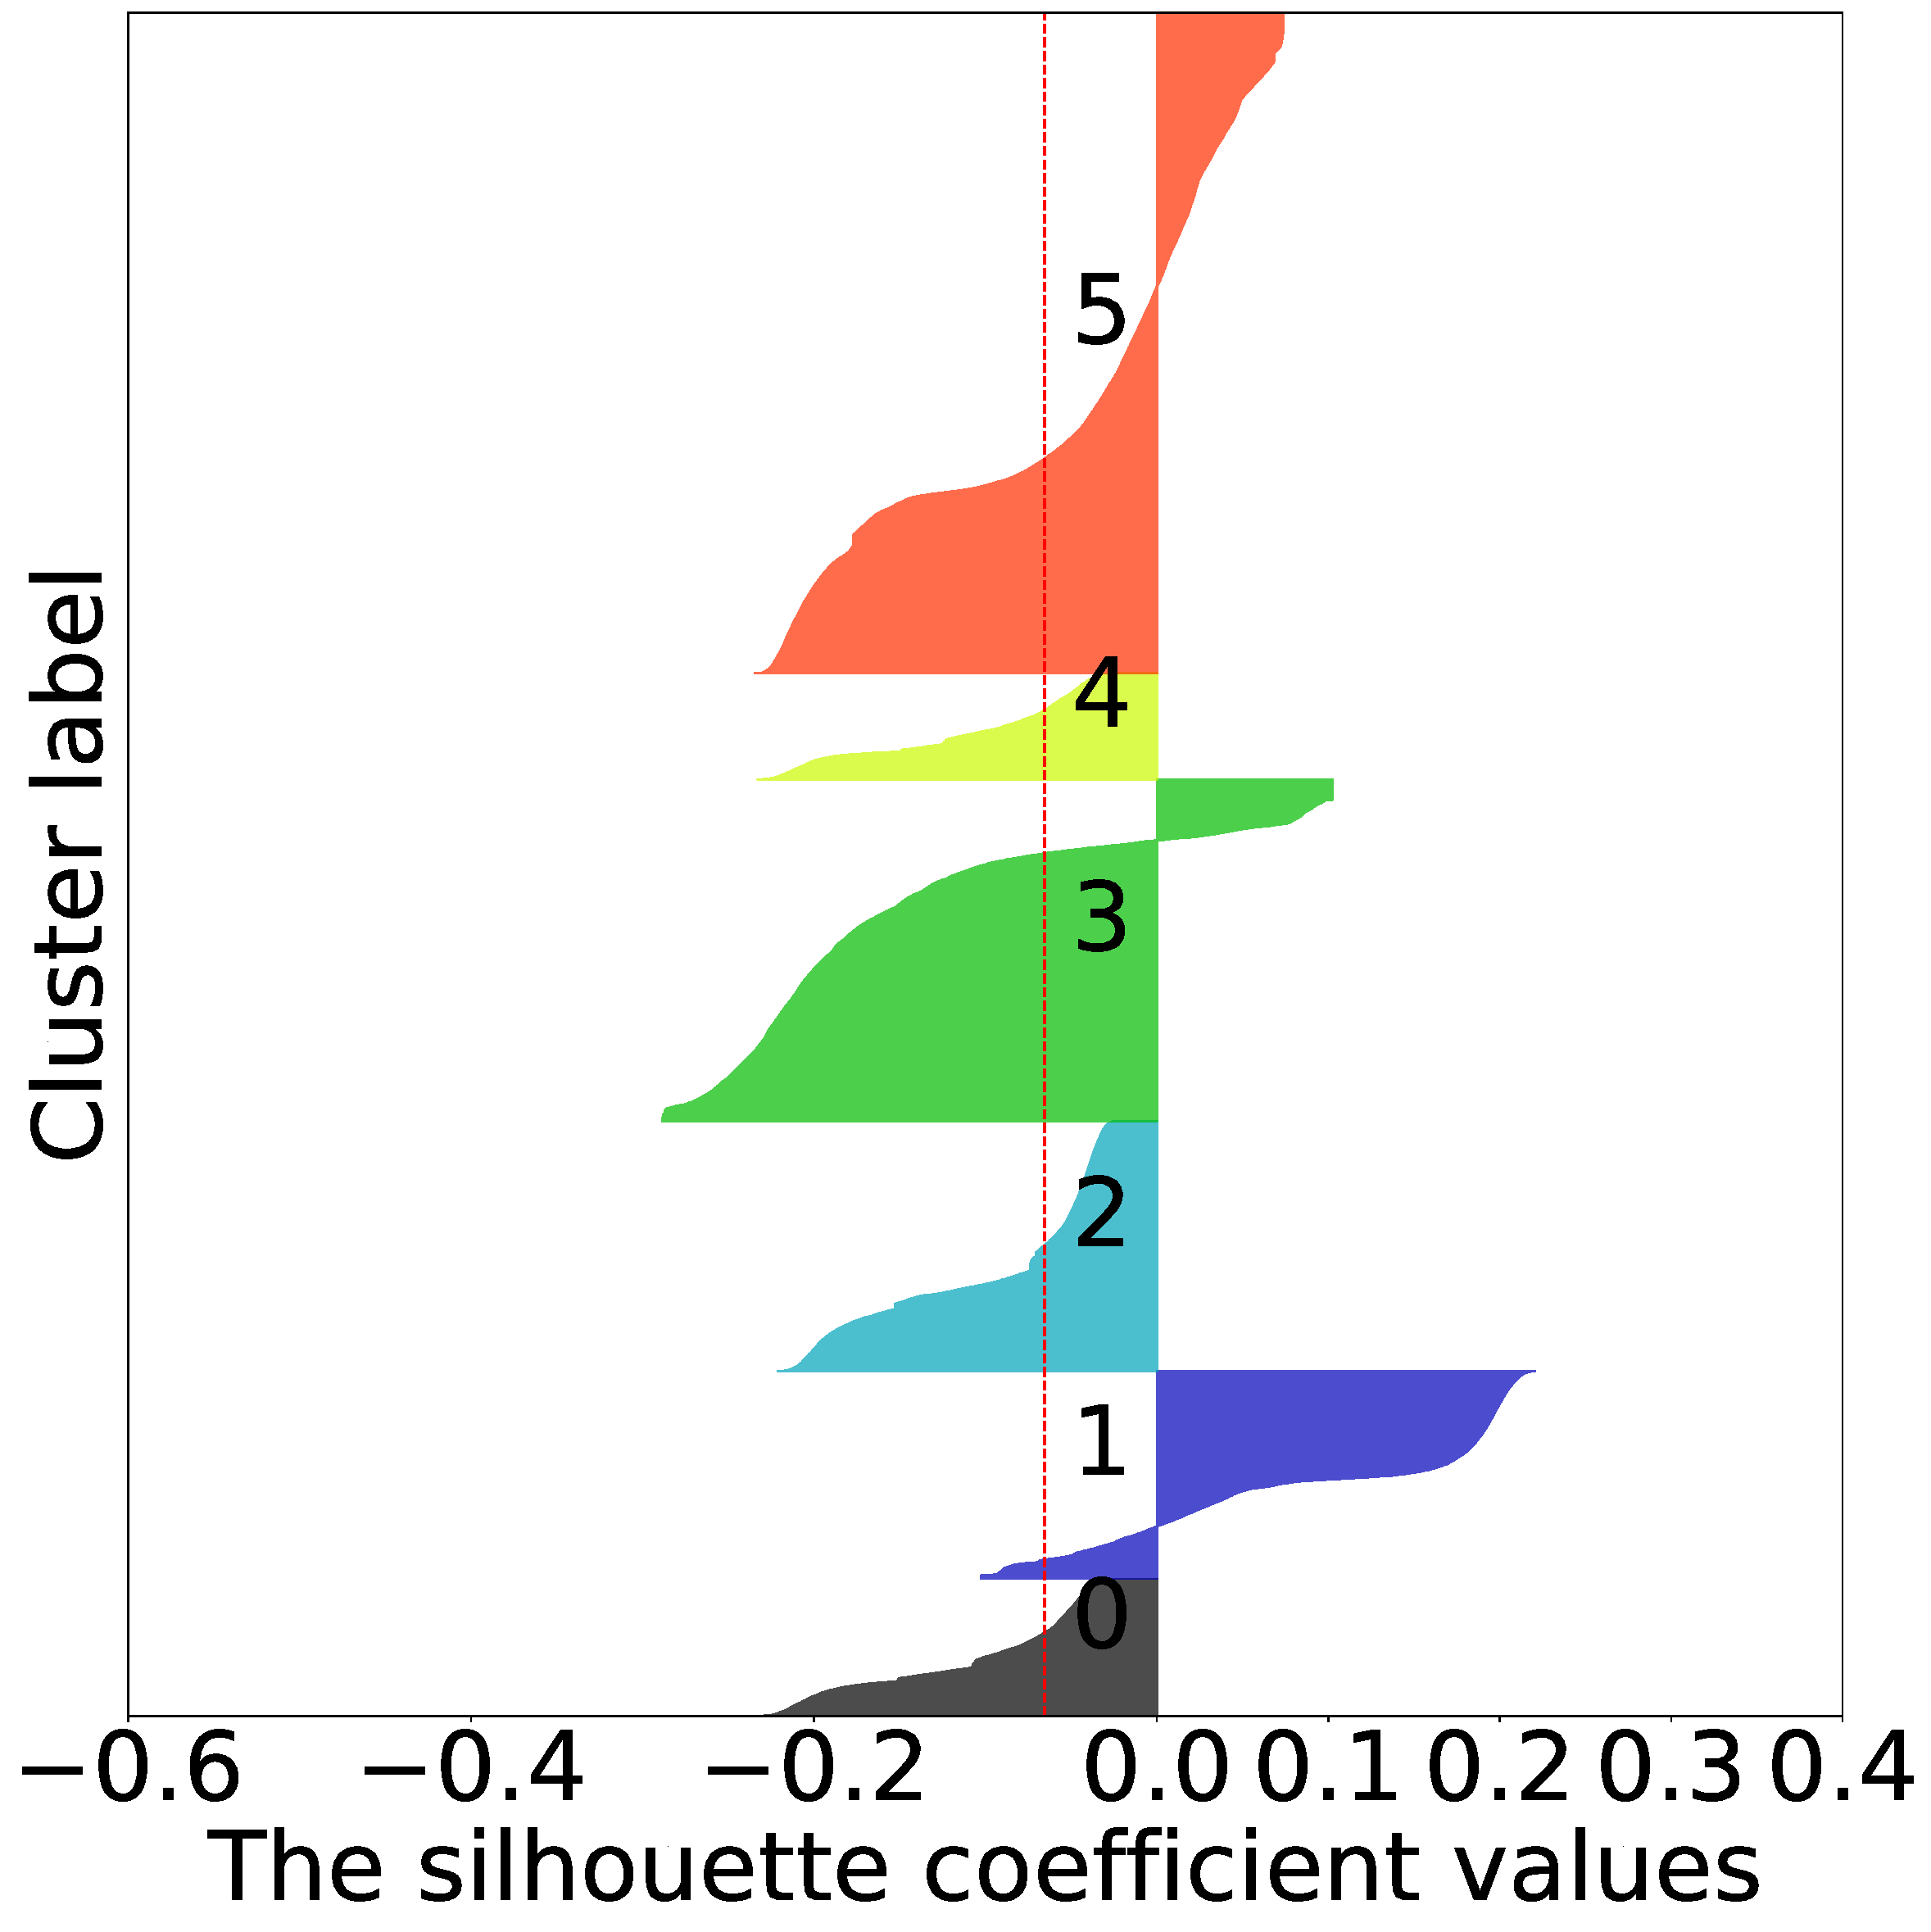
\includegraphics[width=0.33\textwidth]{figures/silhouette/silhouette_directly_6.pdf}
    }
        \subfloat[n\_clusters = 7]{
        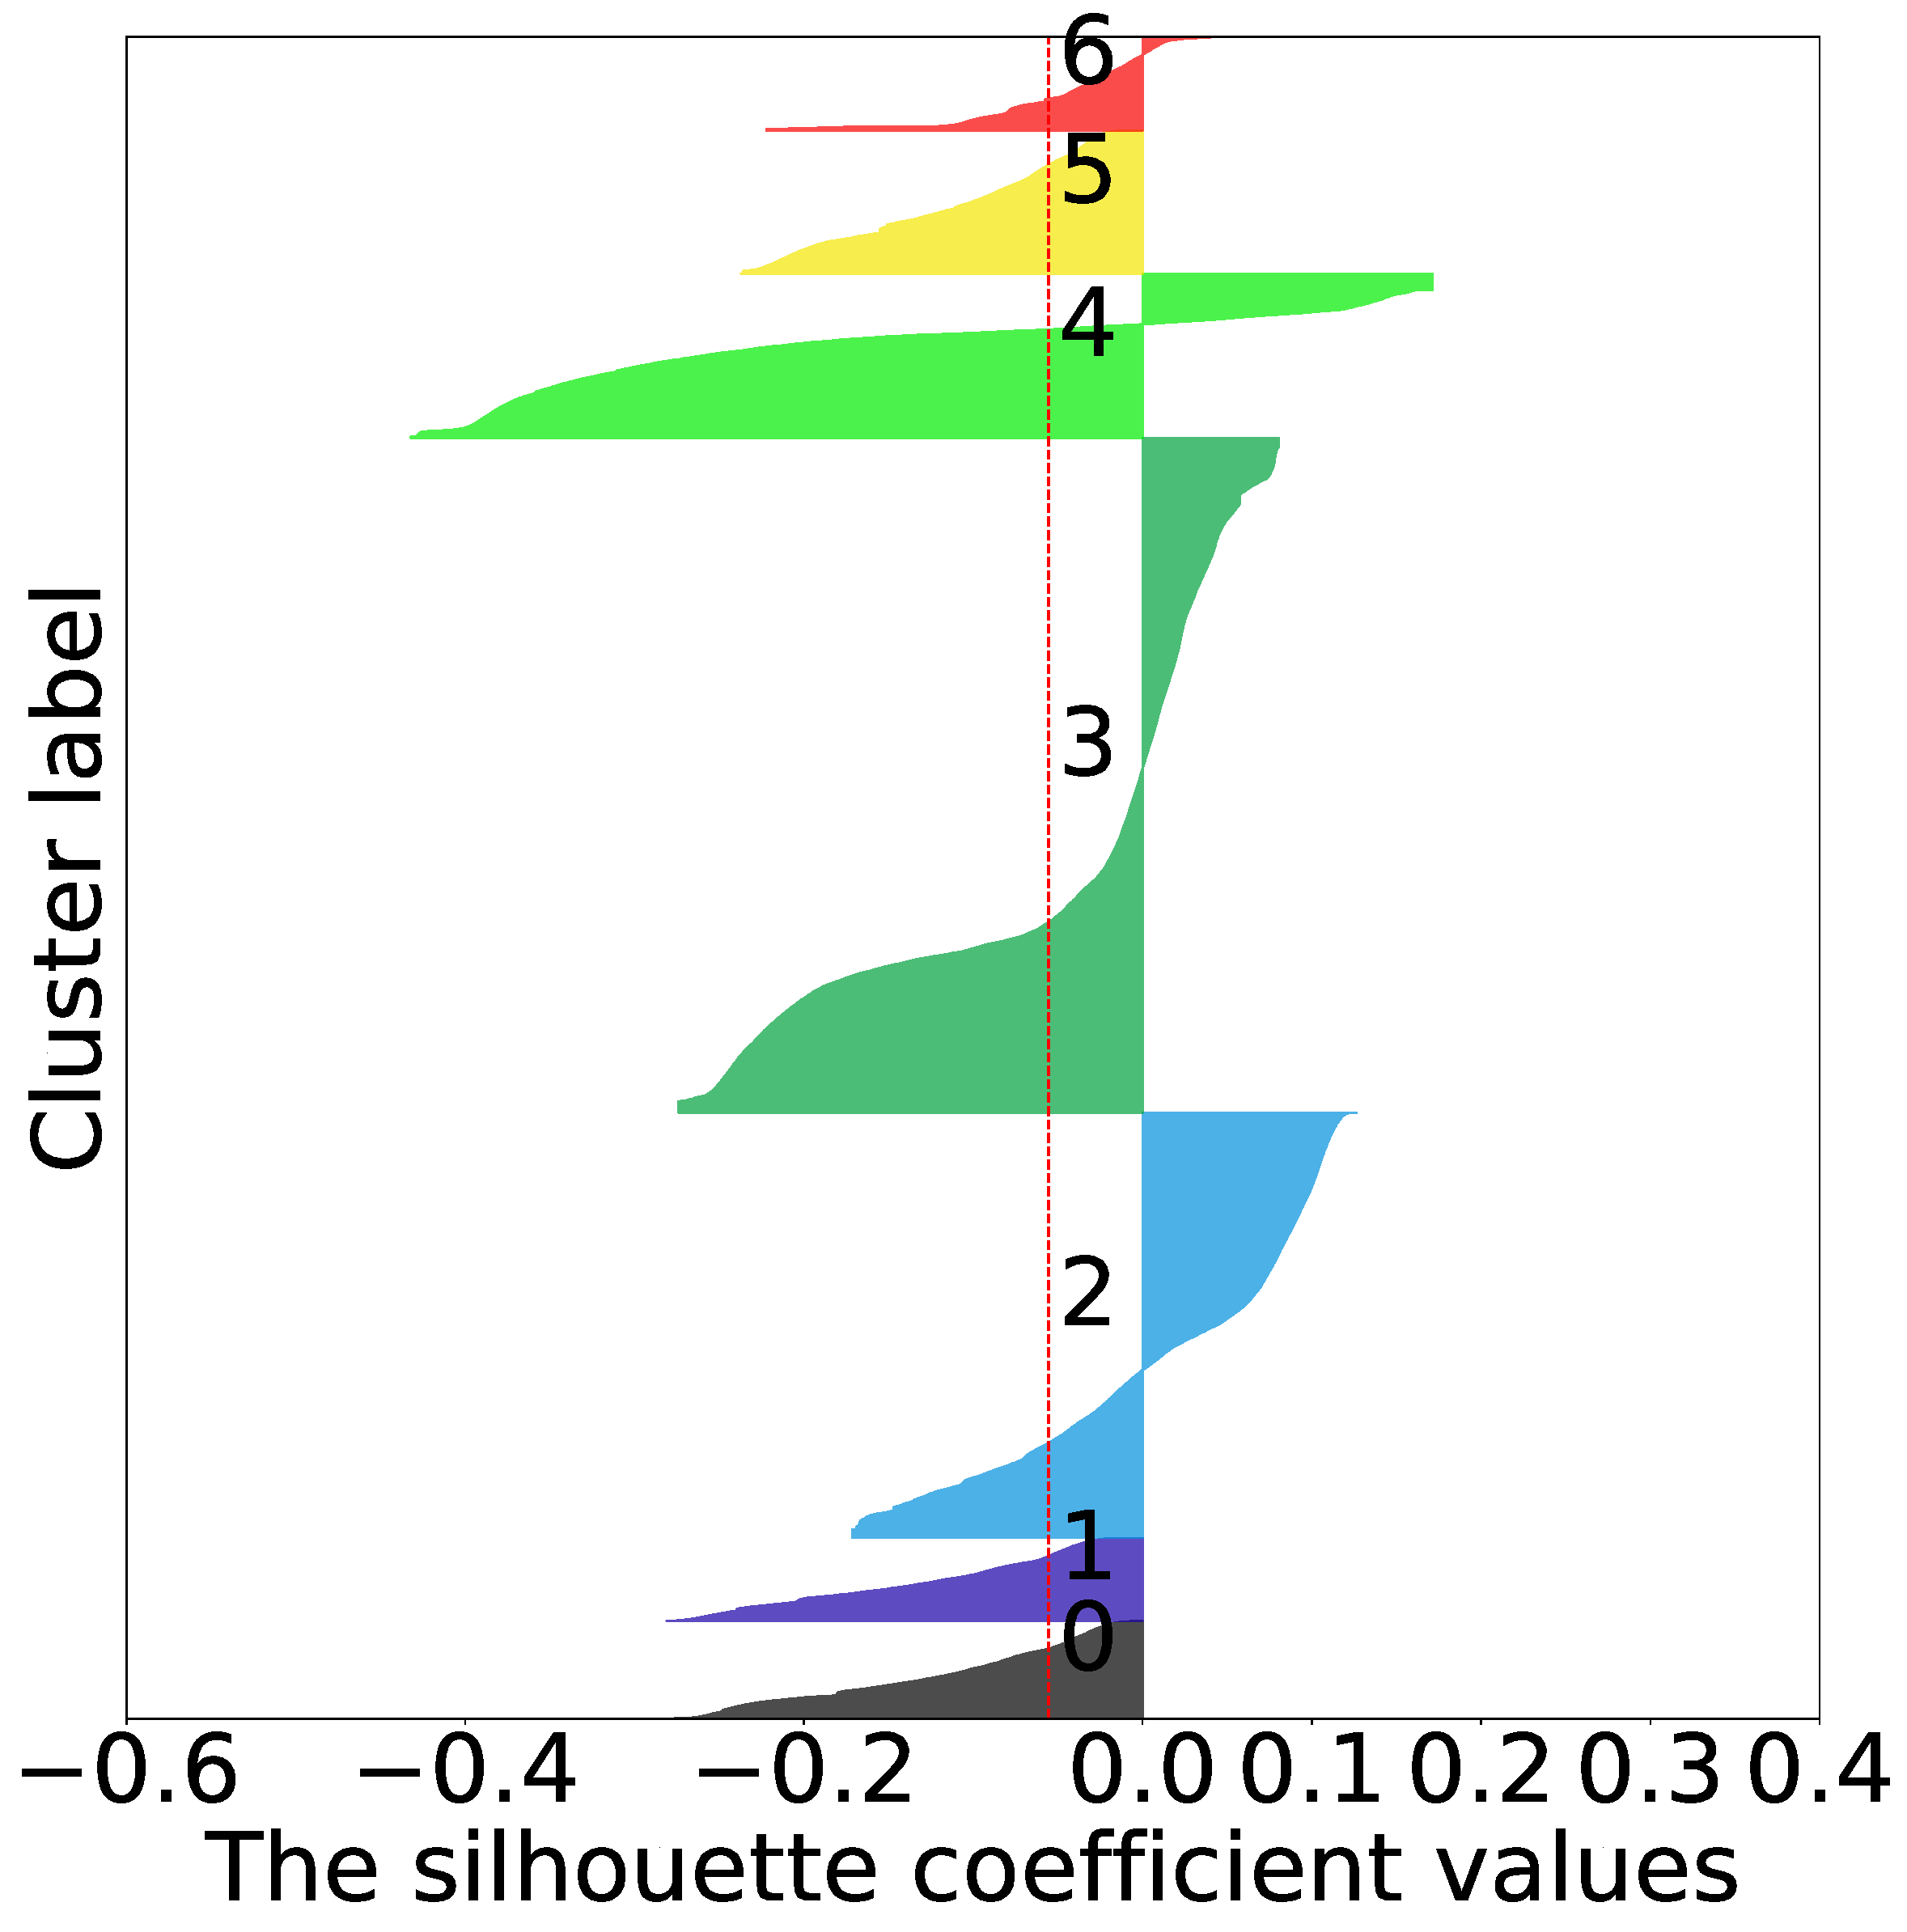
\includegraphics[width=0.33\textwidth]{figures/silhouette/silhouette_directly_7.pdf}
    }\\
        \subfloat[n\_clusters = 8]{
        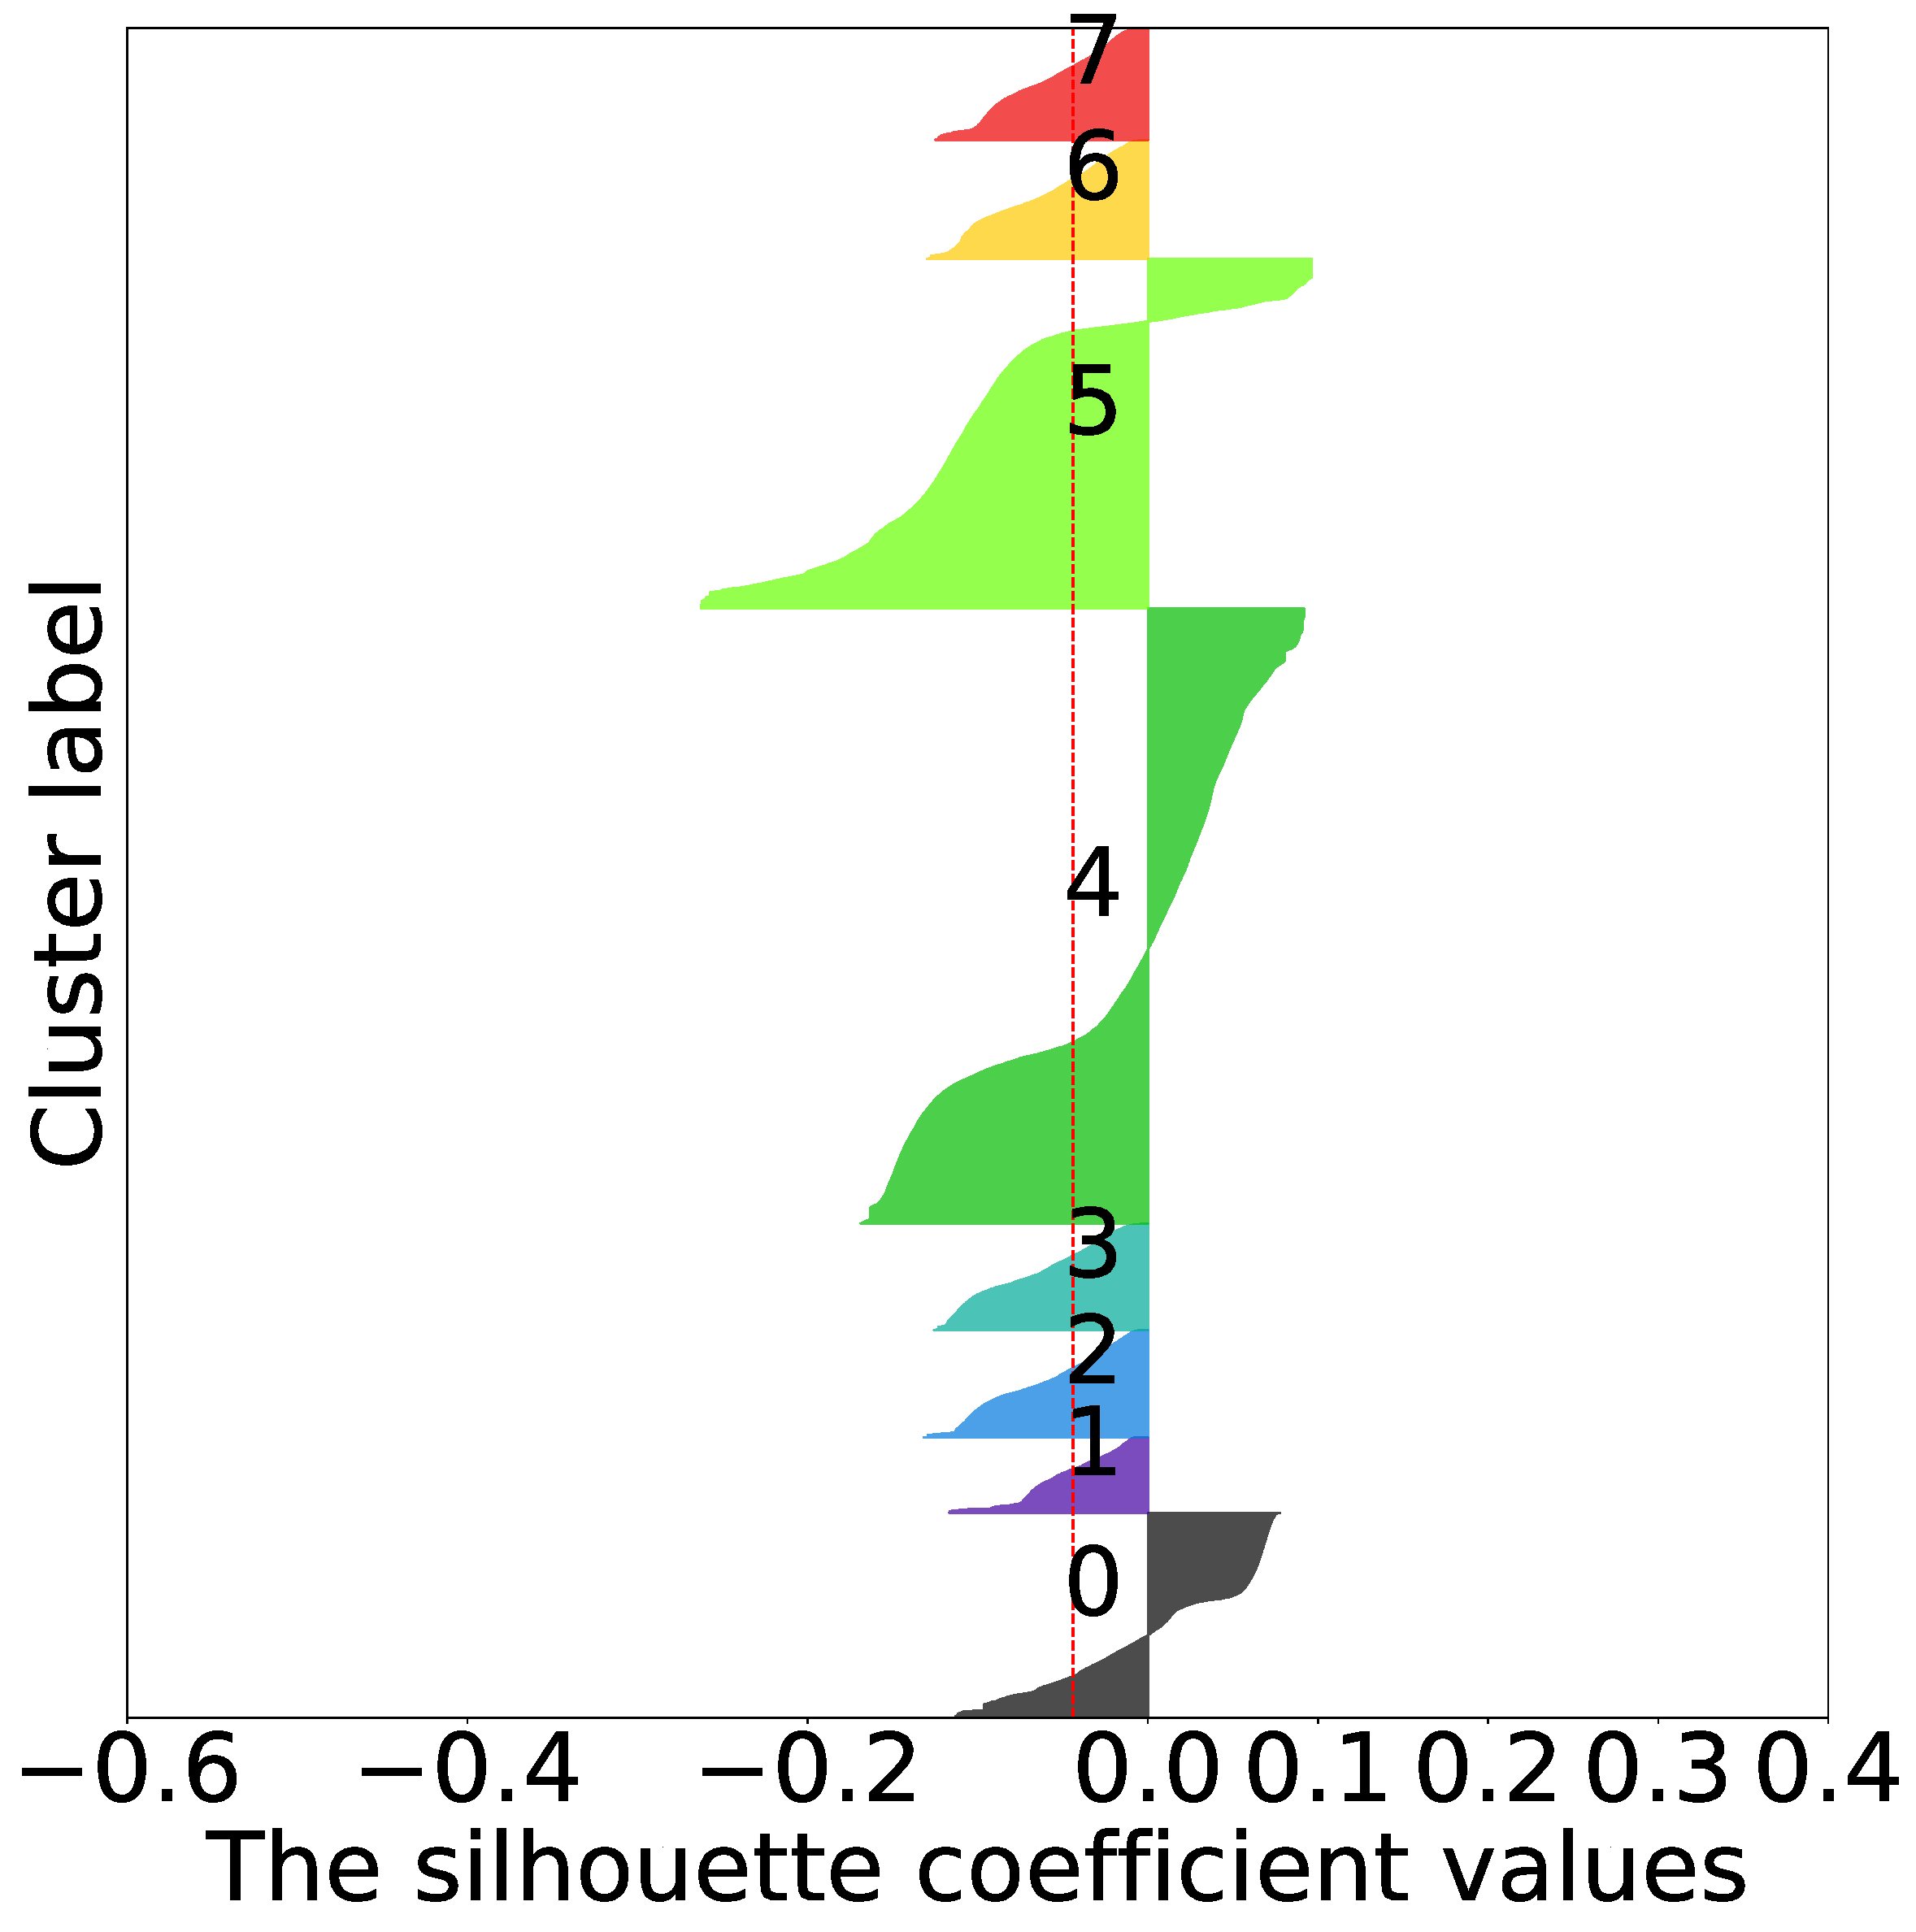
\includegraphics[width=0.33\textwidth]{figures/silhouette/silhouette_directly_8.pdf}
    }
        \subfloat[n\_clusters = 9]{
        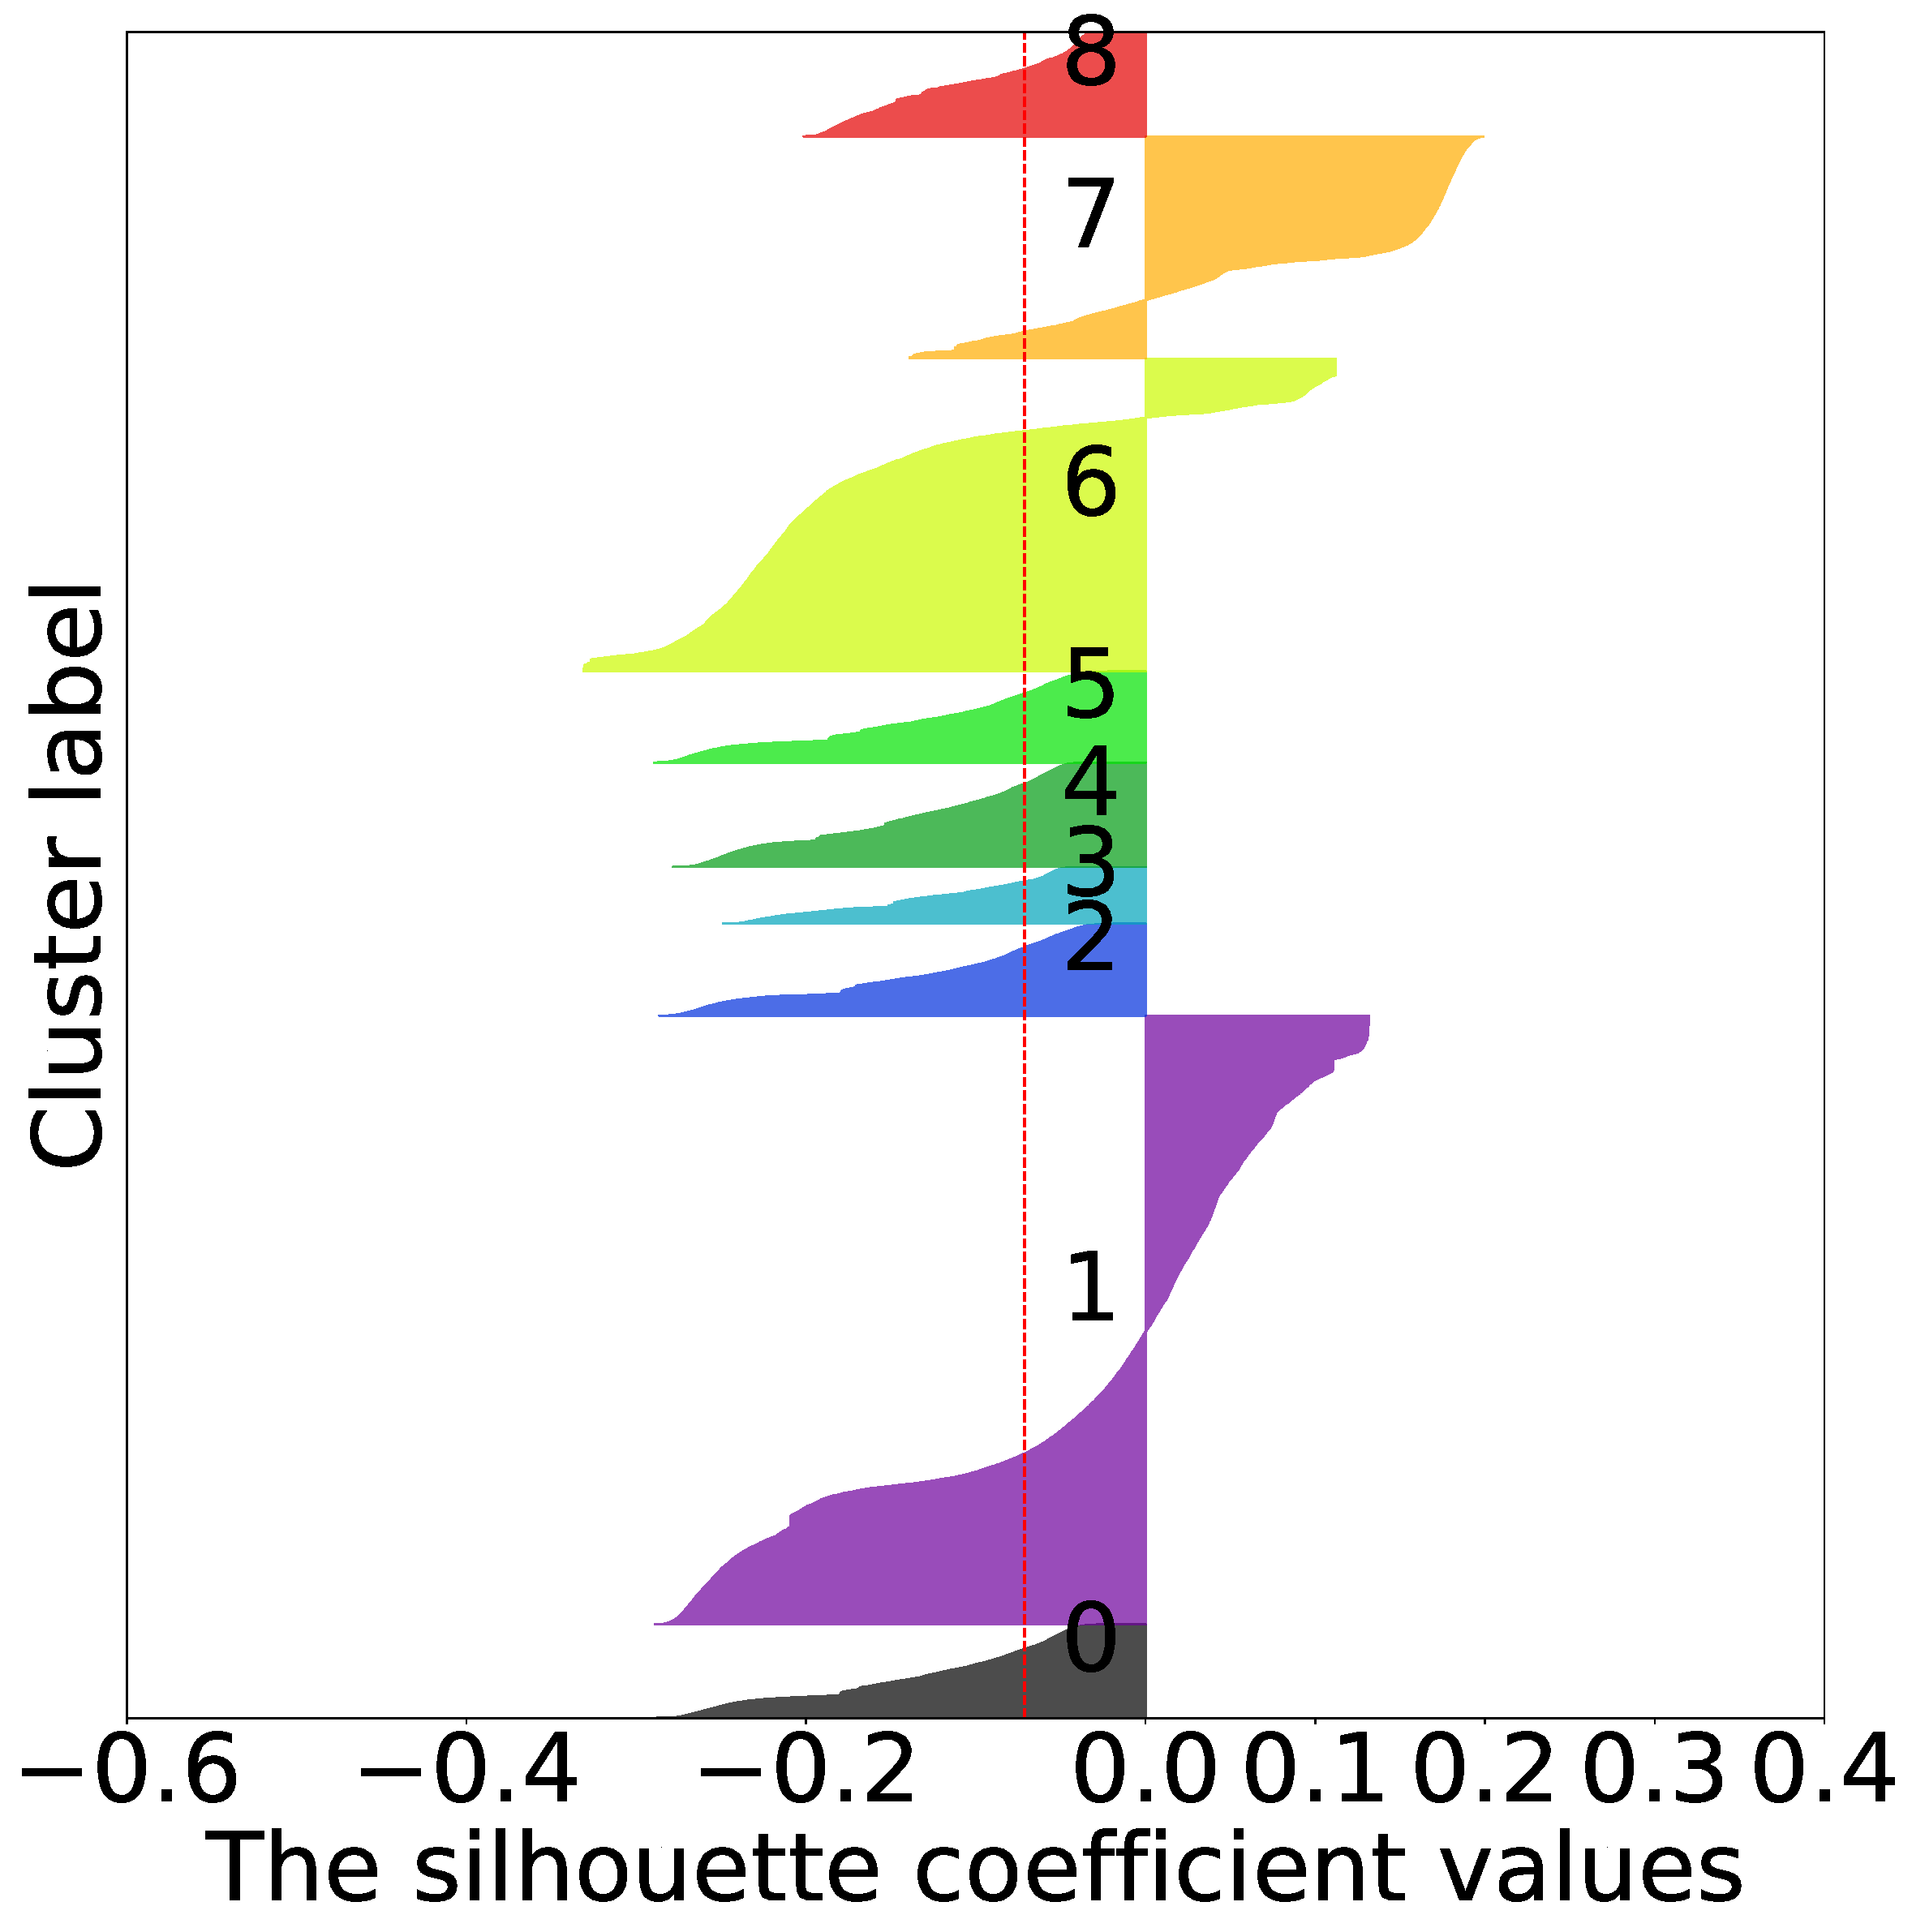
\includegraphics[width=0.33\textwidth]{figures/silhouette/silhouette_directly_9.pdf}
    }
        \subfloat[n\_clusters = 10]{
        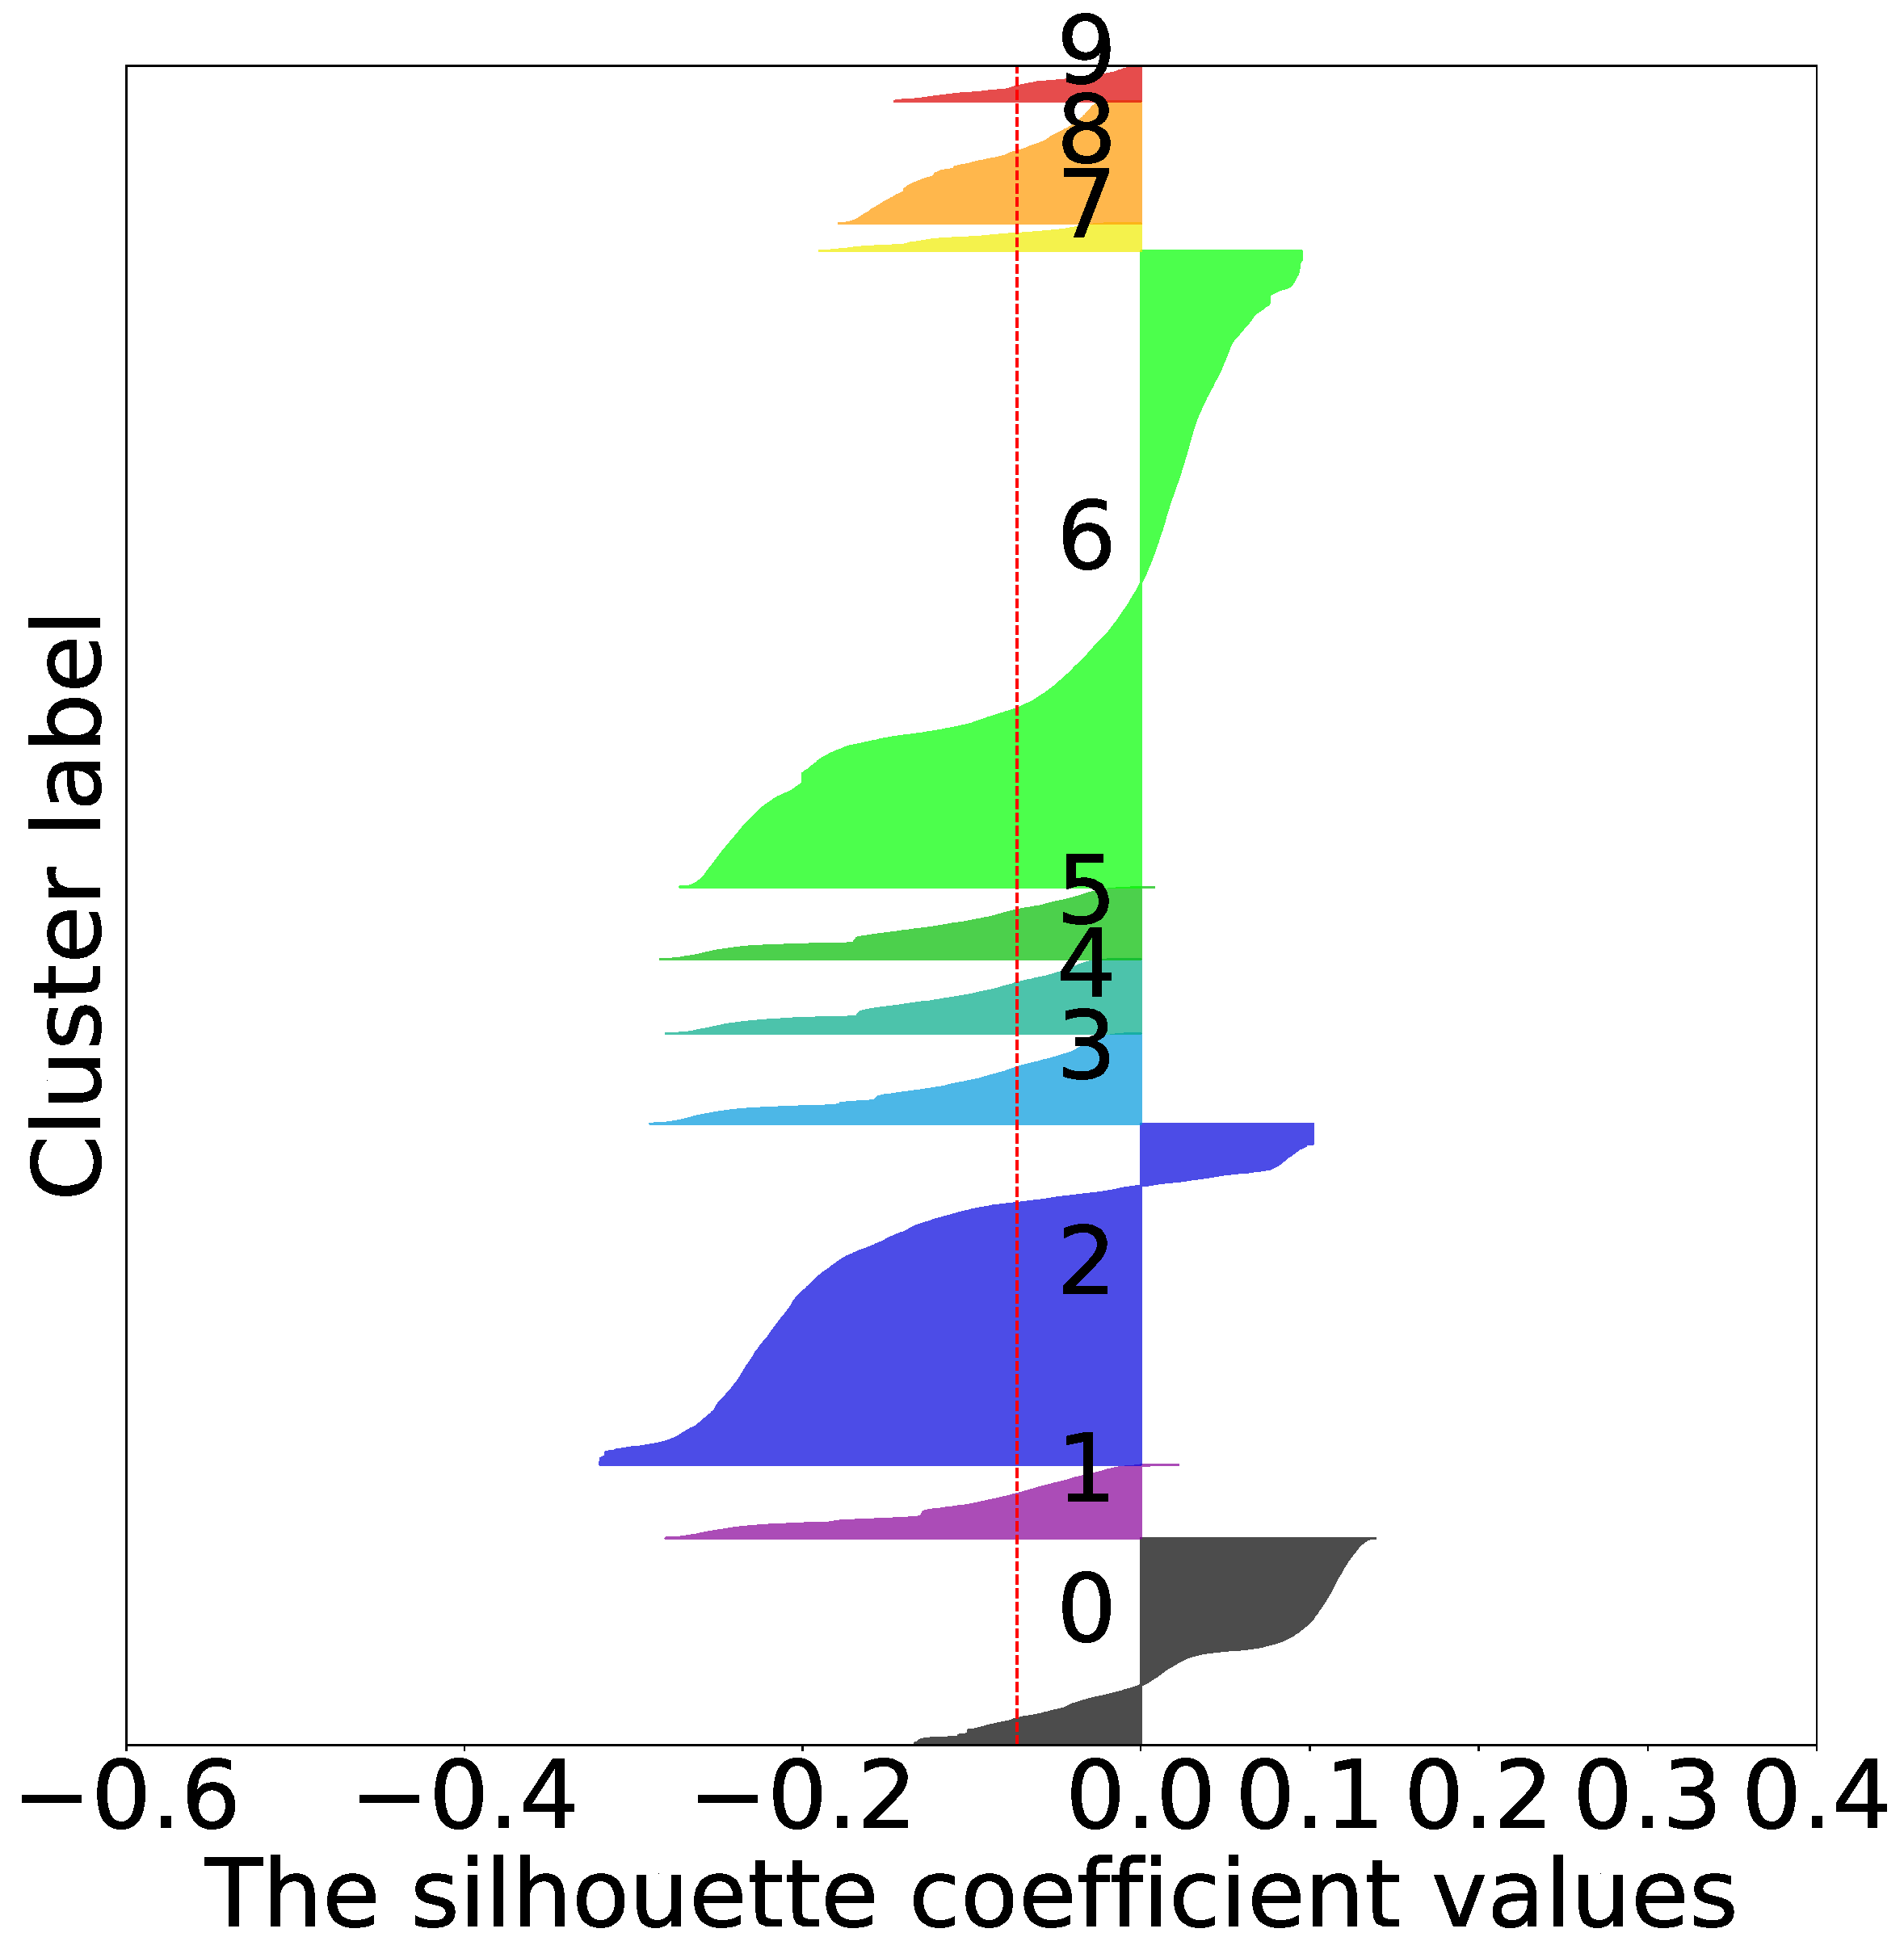
\includegraphics[width=0.33\textwidth]{figures/silhouette/silhouette_directly_10.pdf}
    }
    \caption{Silhouette analysis for KMeans clustering on windowed time-series data directly}
    \label{fig_silhouette_directly}
\end{figure}

\begin{figure}[H]
    \centering
        \subfloat[n\_clusters = 2]{
        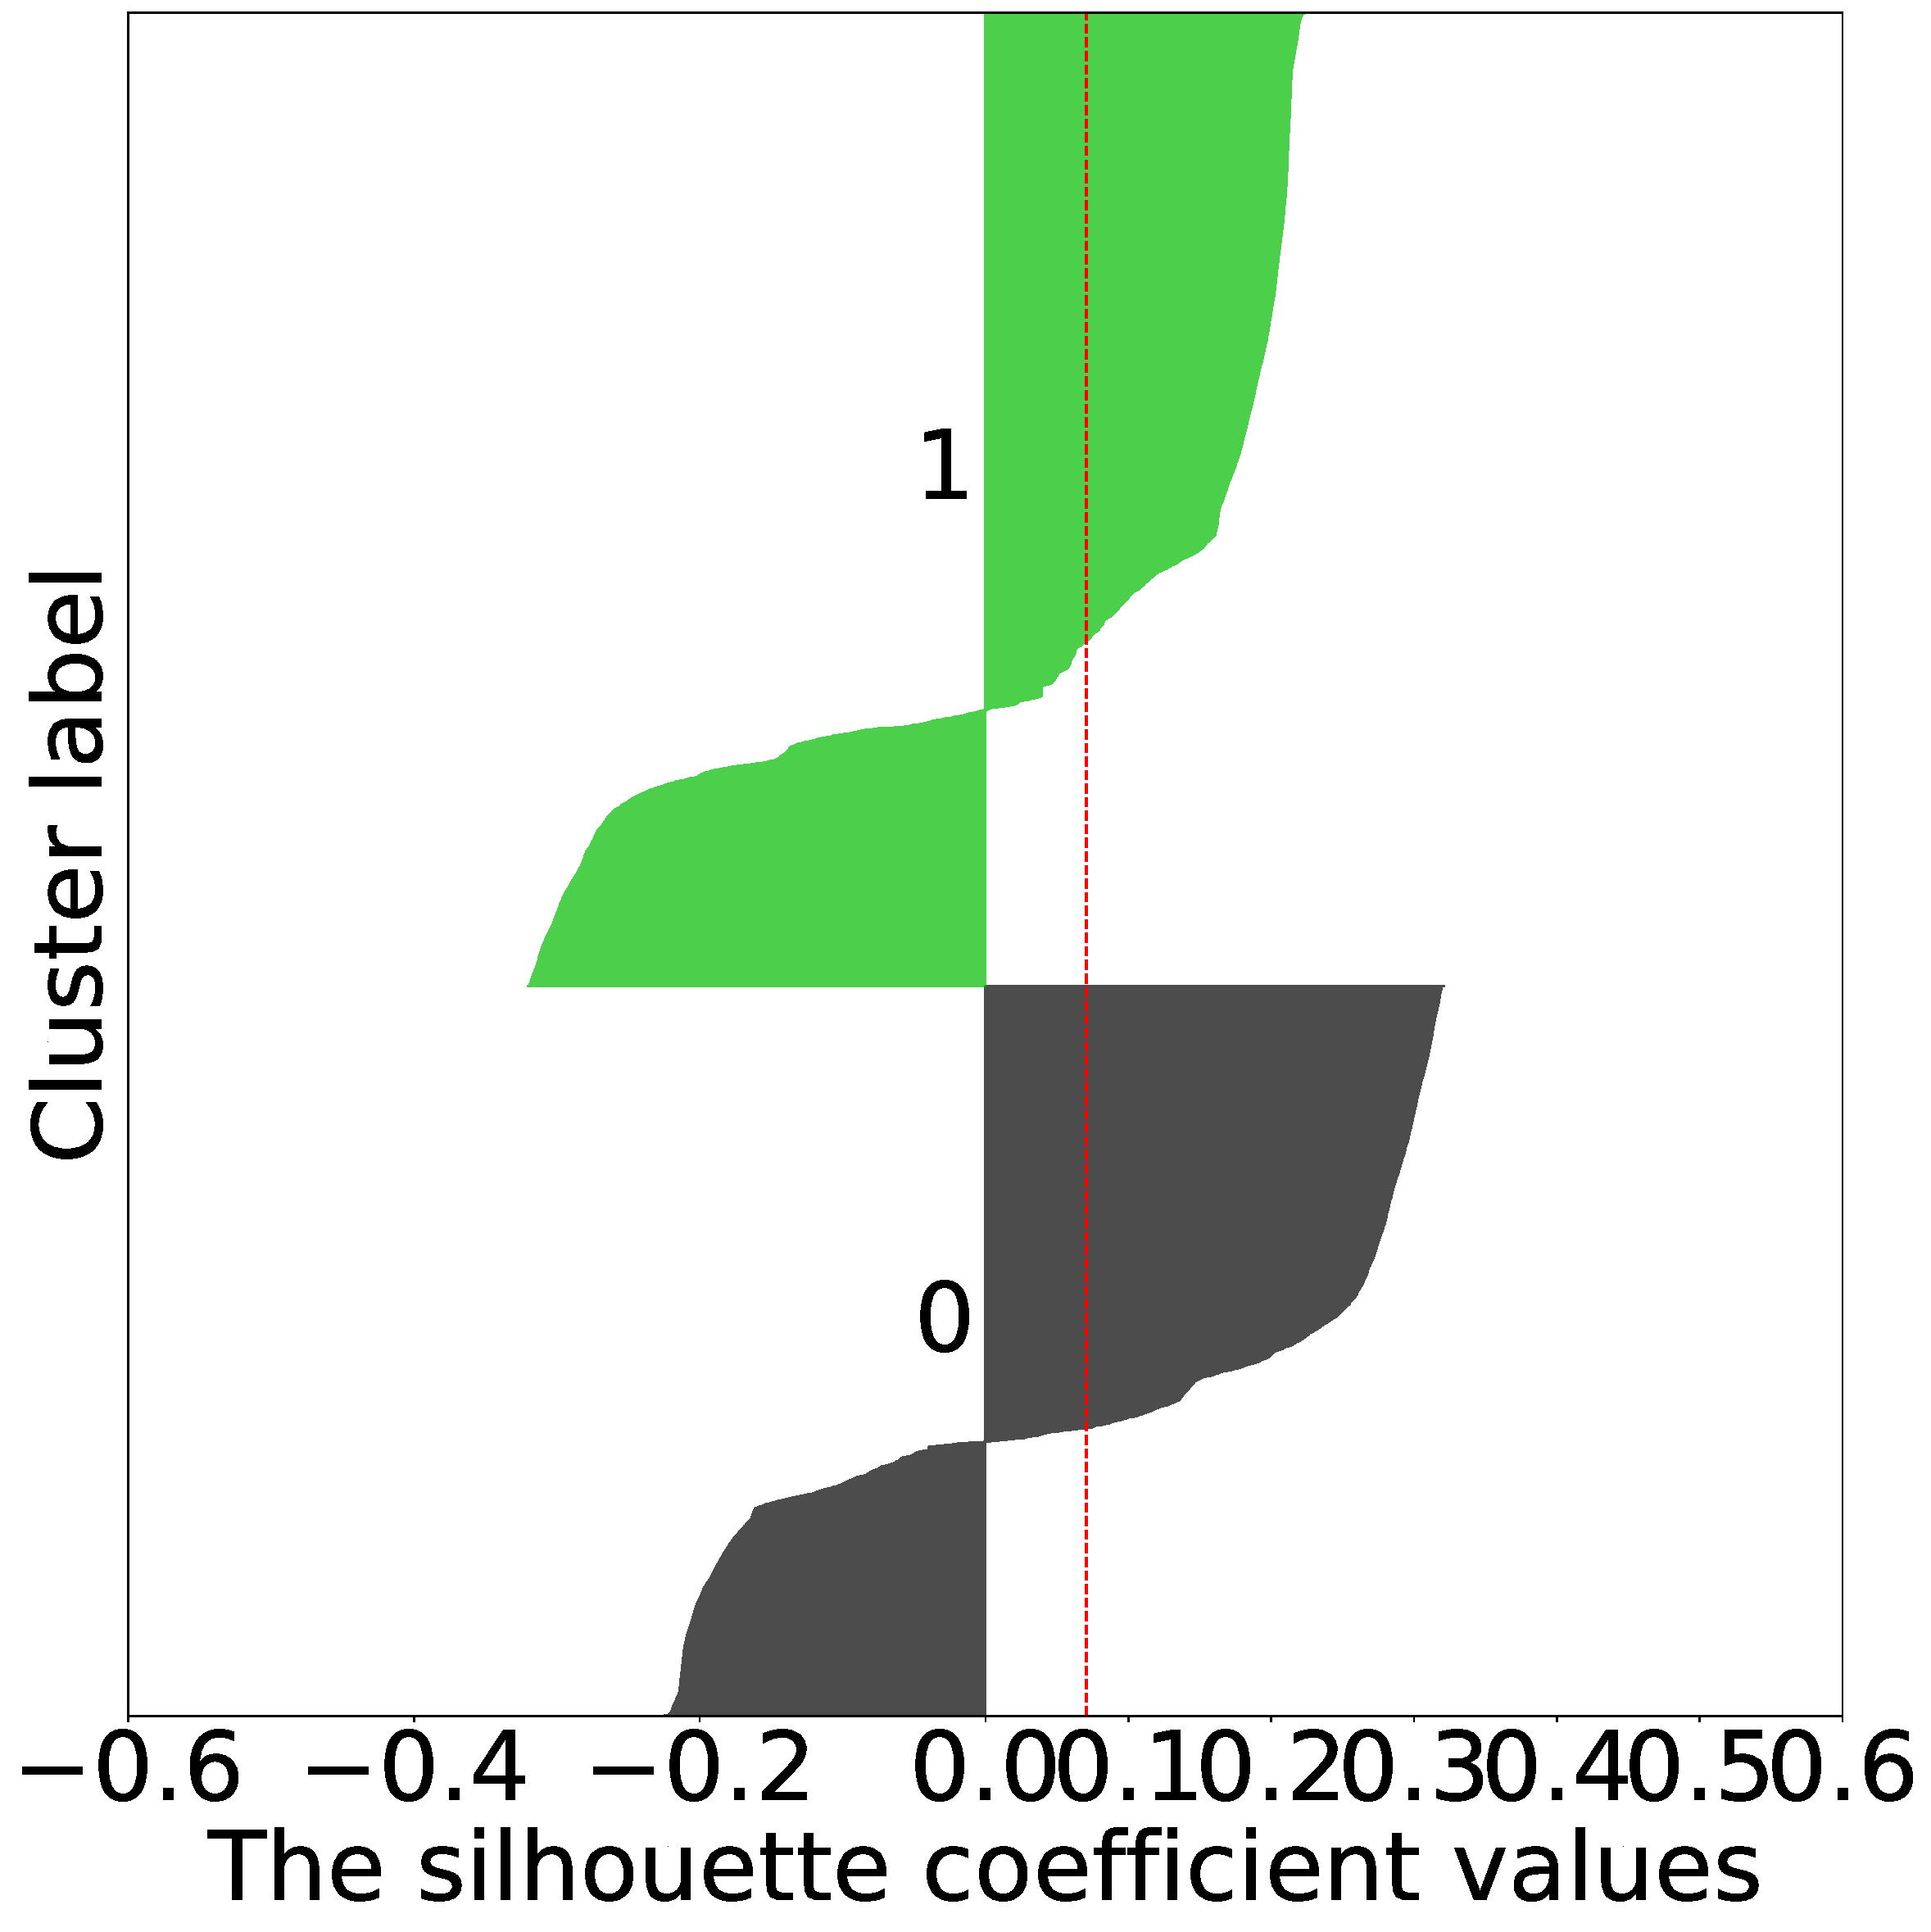
\includegraphics[width=0.33\textwidth]{figures/silhouette/silhouette_statistics_2.pdf}
    }
        \subfloat[n\_clusters = 3]{
        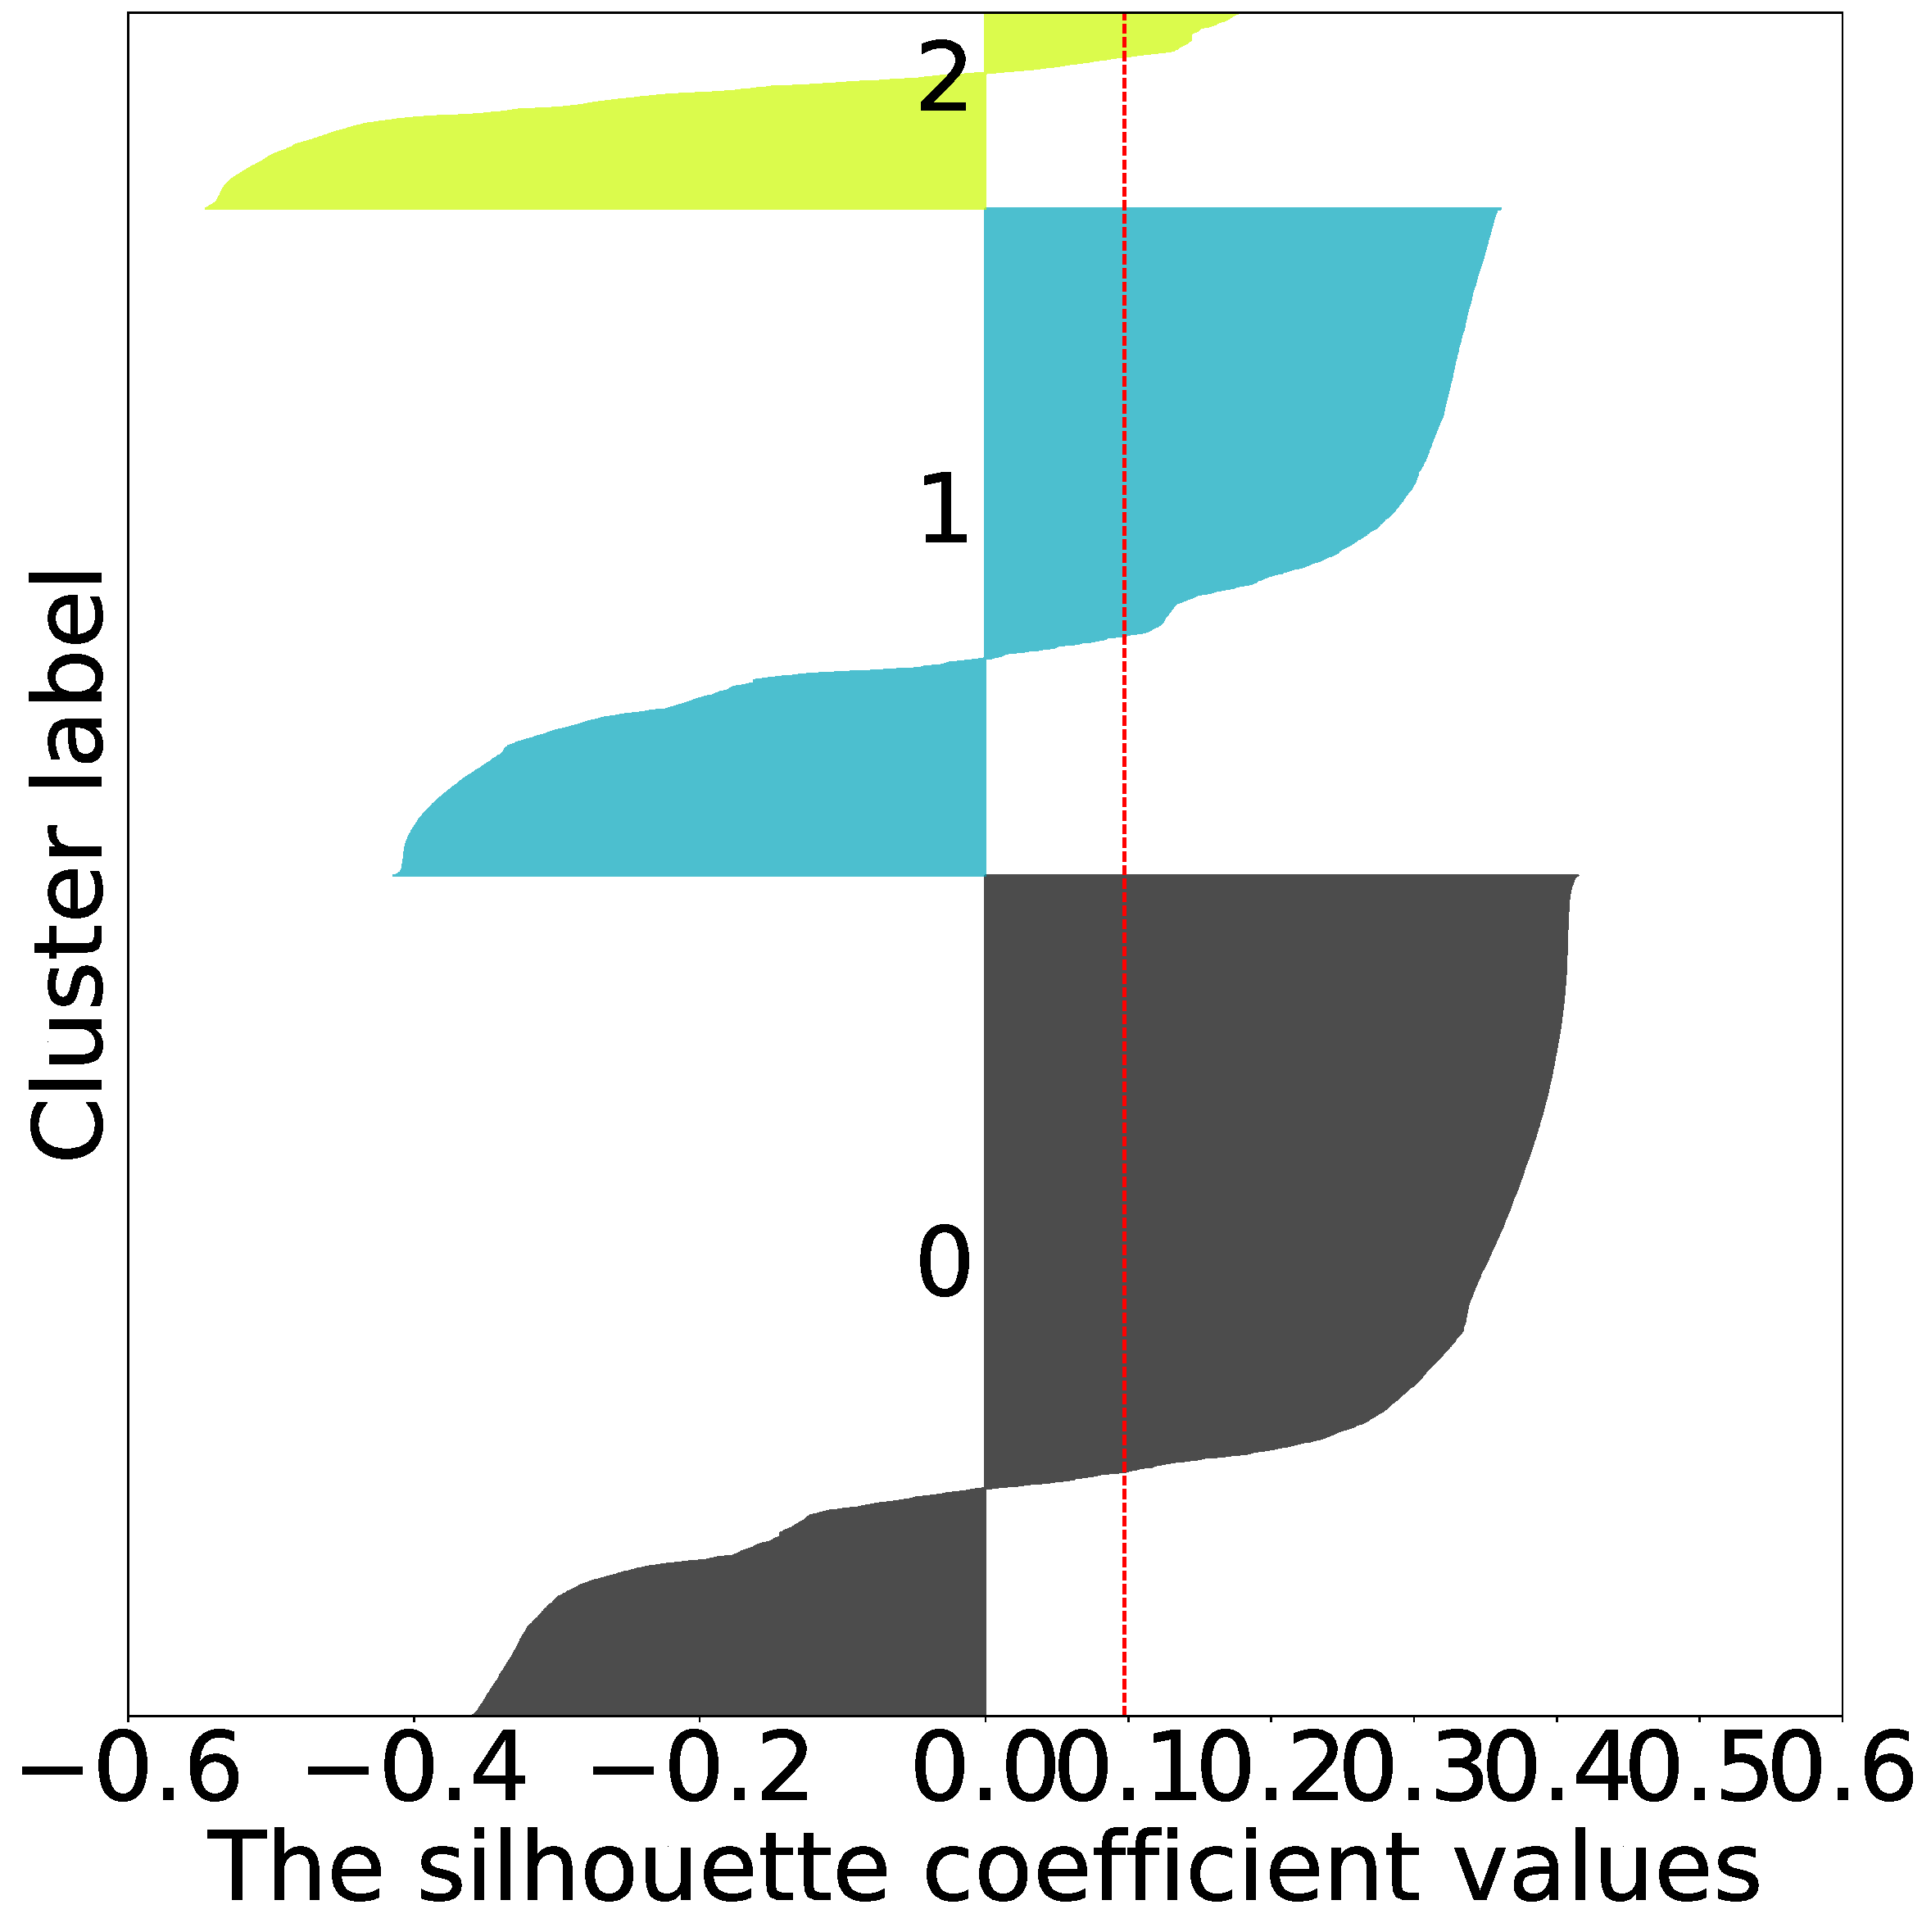
\includegraphics[width=0.33\textwidth]{figures/silhouette/silhouette_statistics_3.pdf}
    }
        \subfloat[n\_clusters = 4]{
        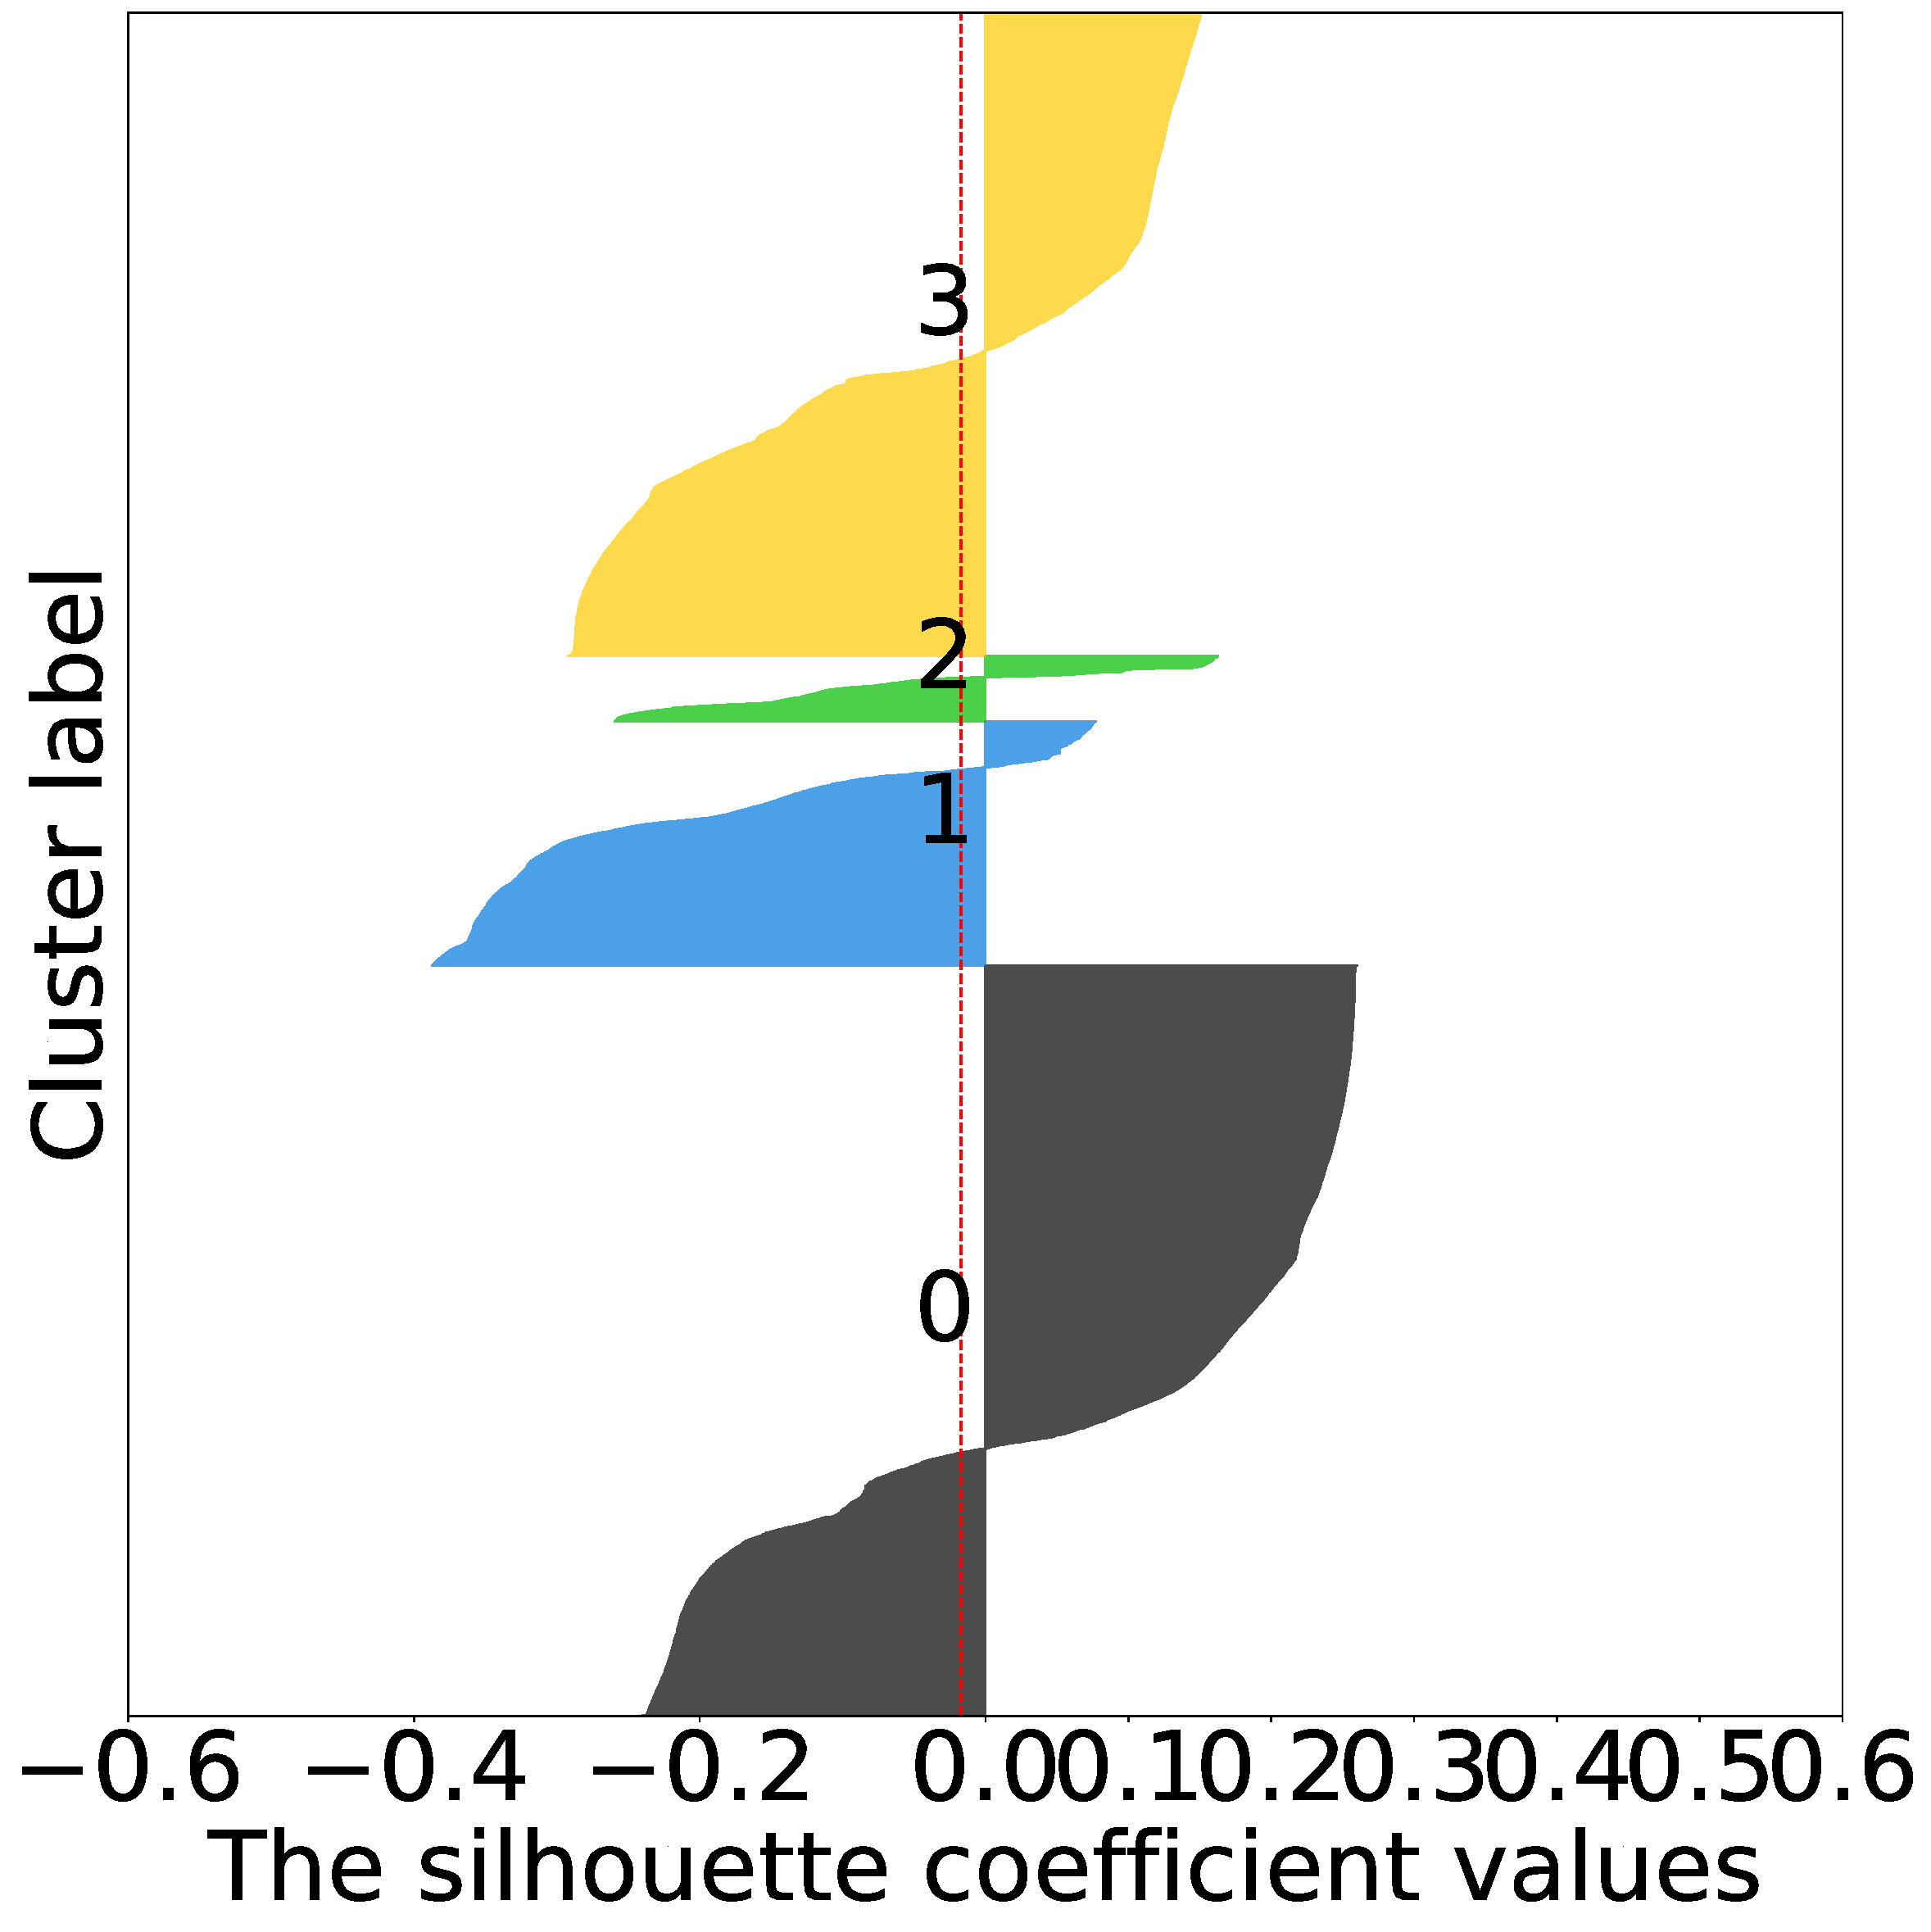
\includegraphics[width=0.33\textwidth]{figures/silhouette/silhouette_statistics_4.pdf}
    }\\
        \subfloat[n\_clusters = 5]{
        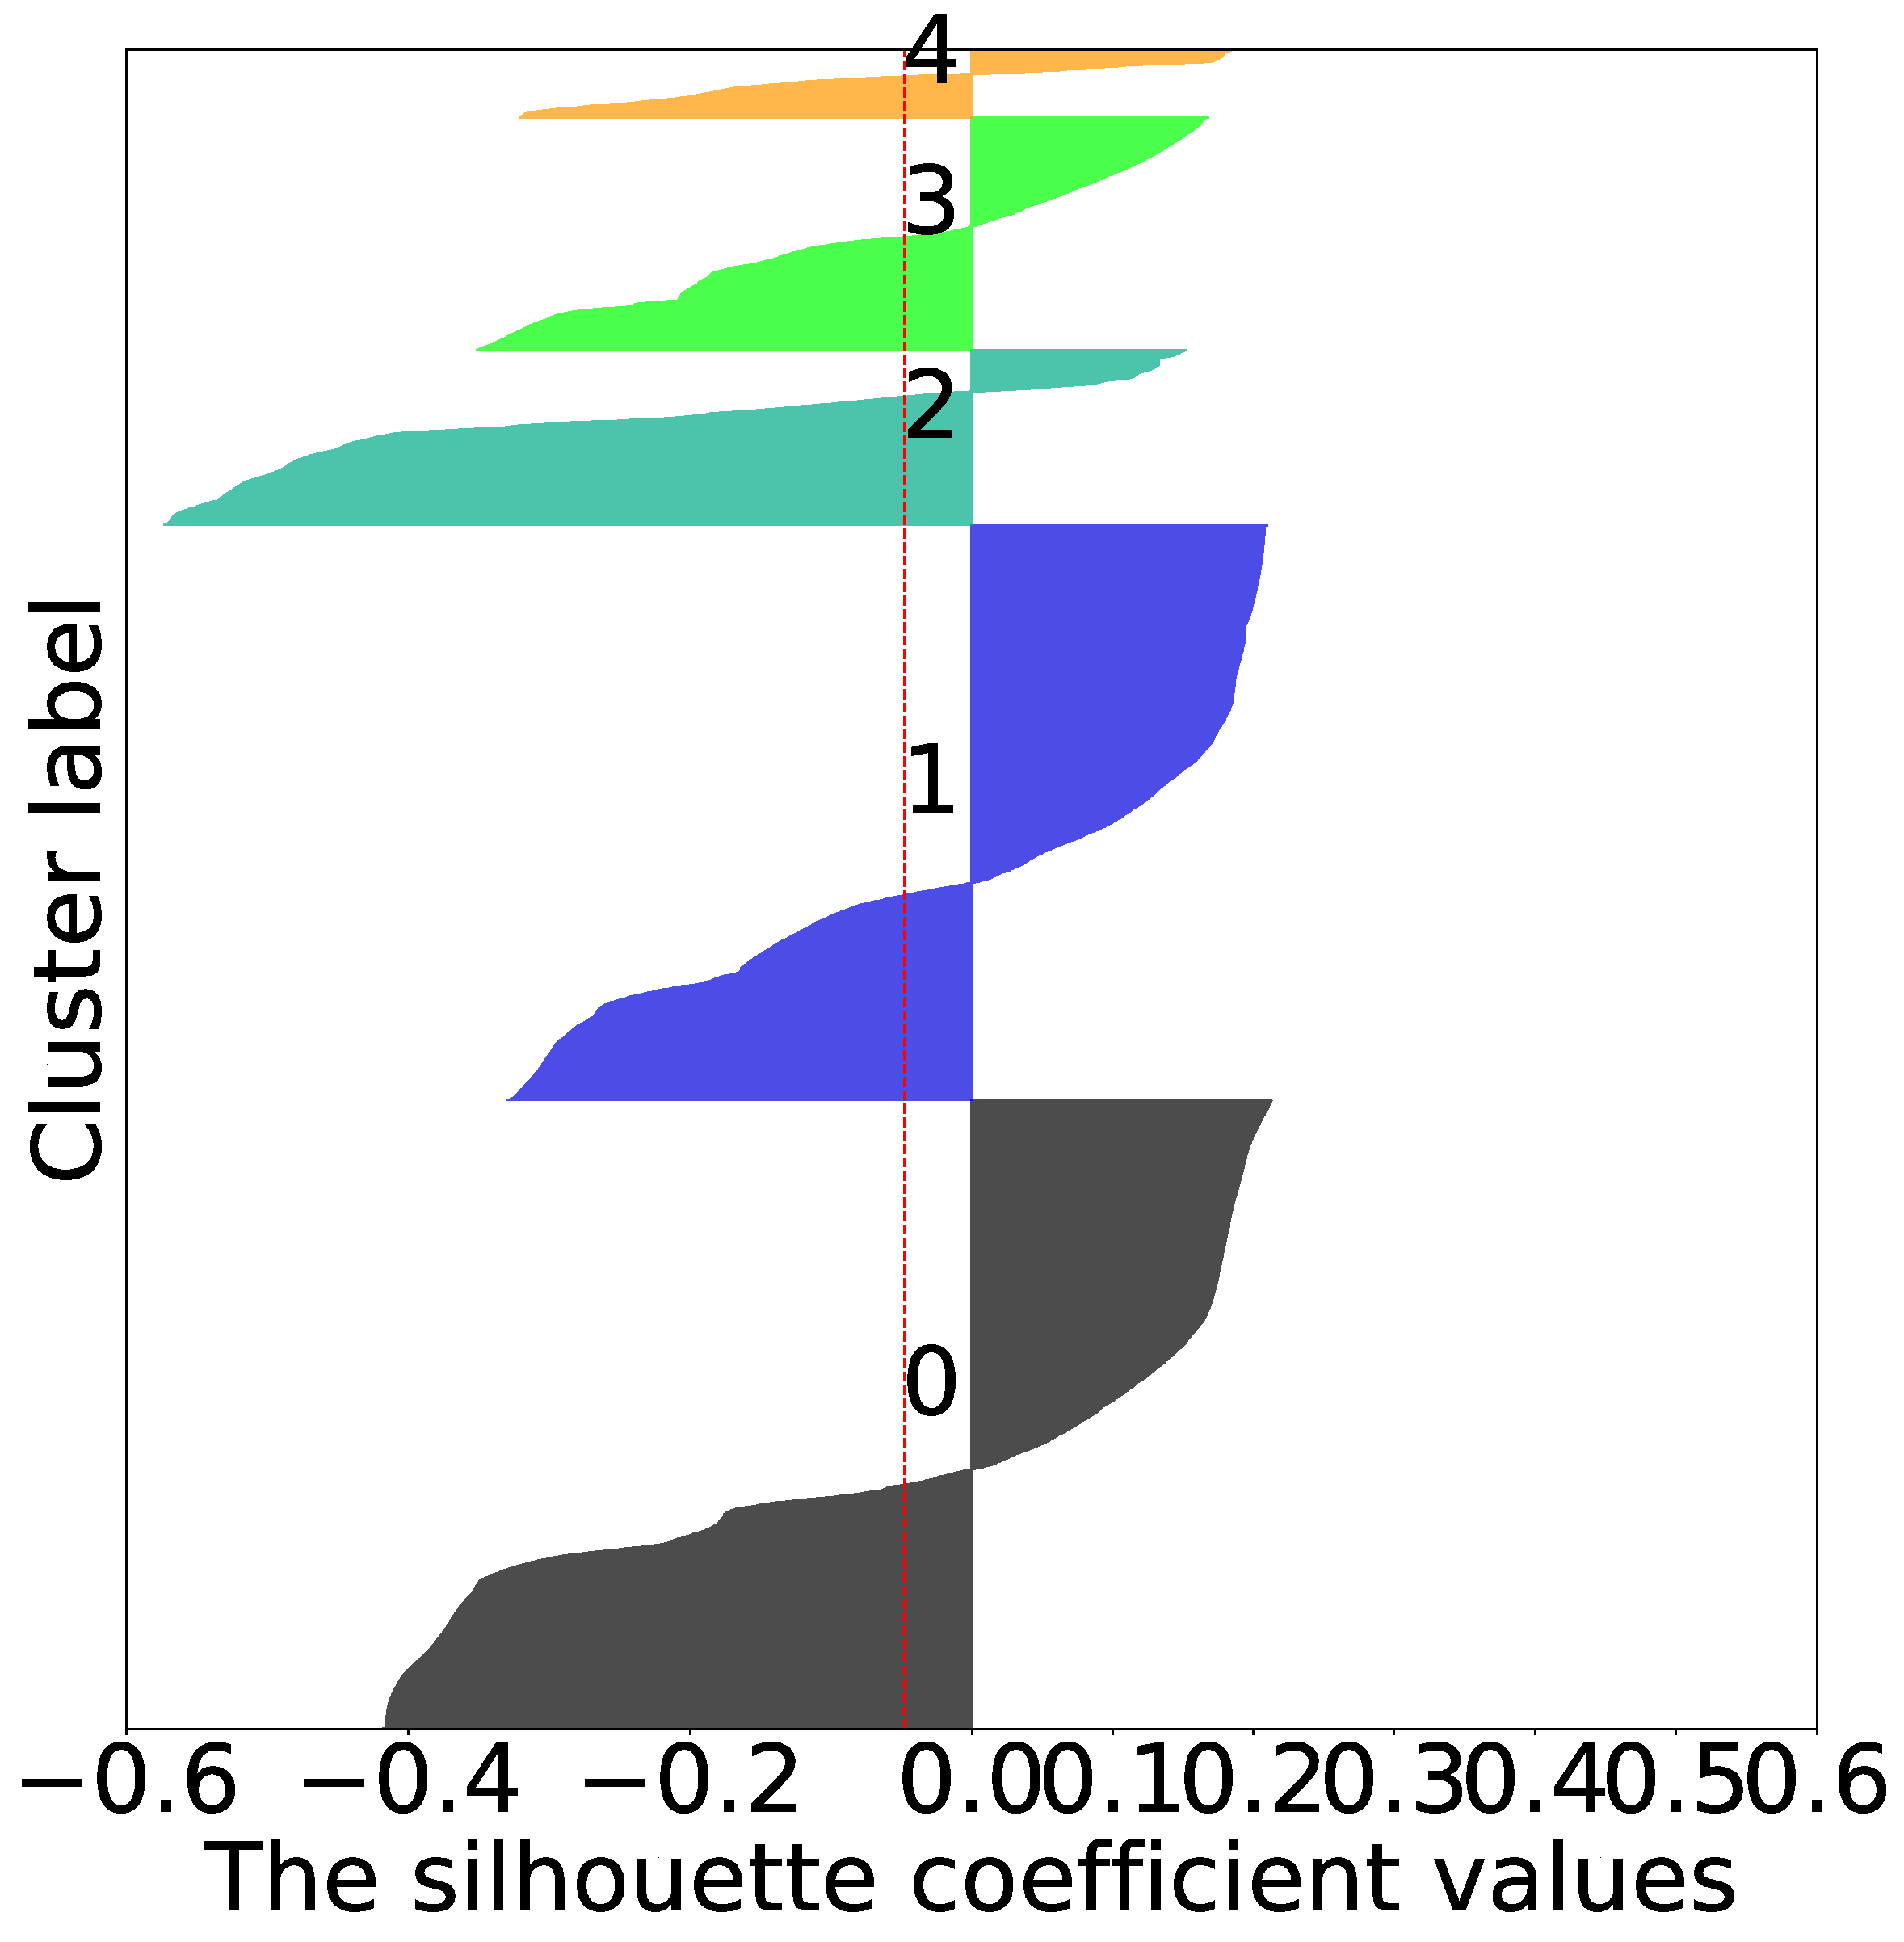
\includegraphics[width=0.33\textwidth]{figures/silhouette/silhouette_statistics_5.pdf}
    }
        \subfloat[n\_clusters = 6]{
        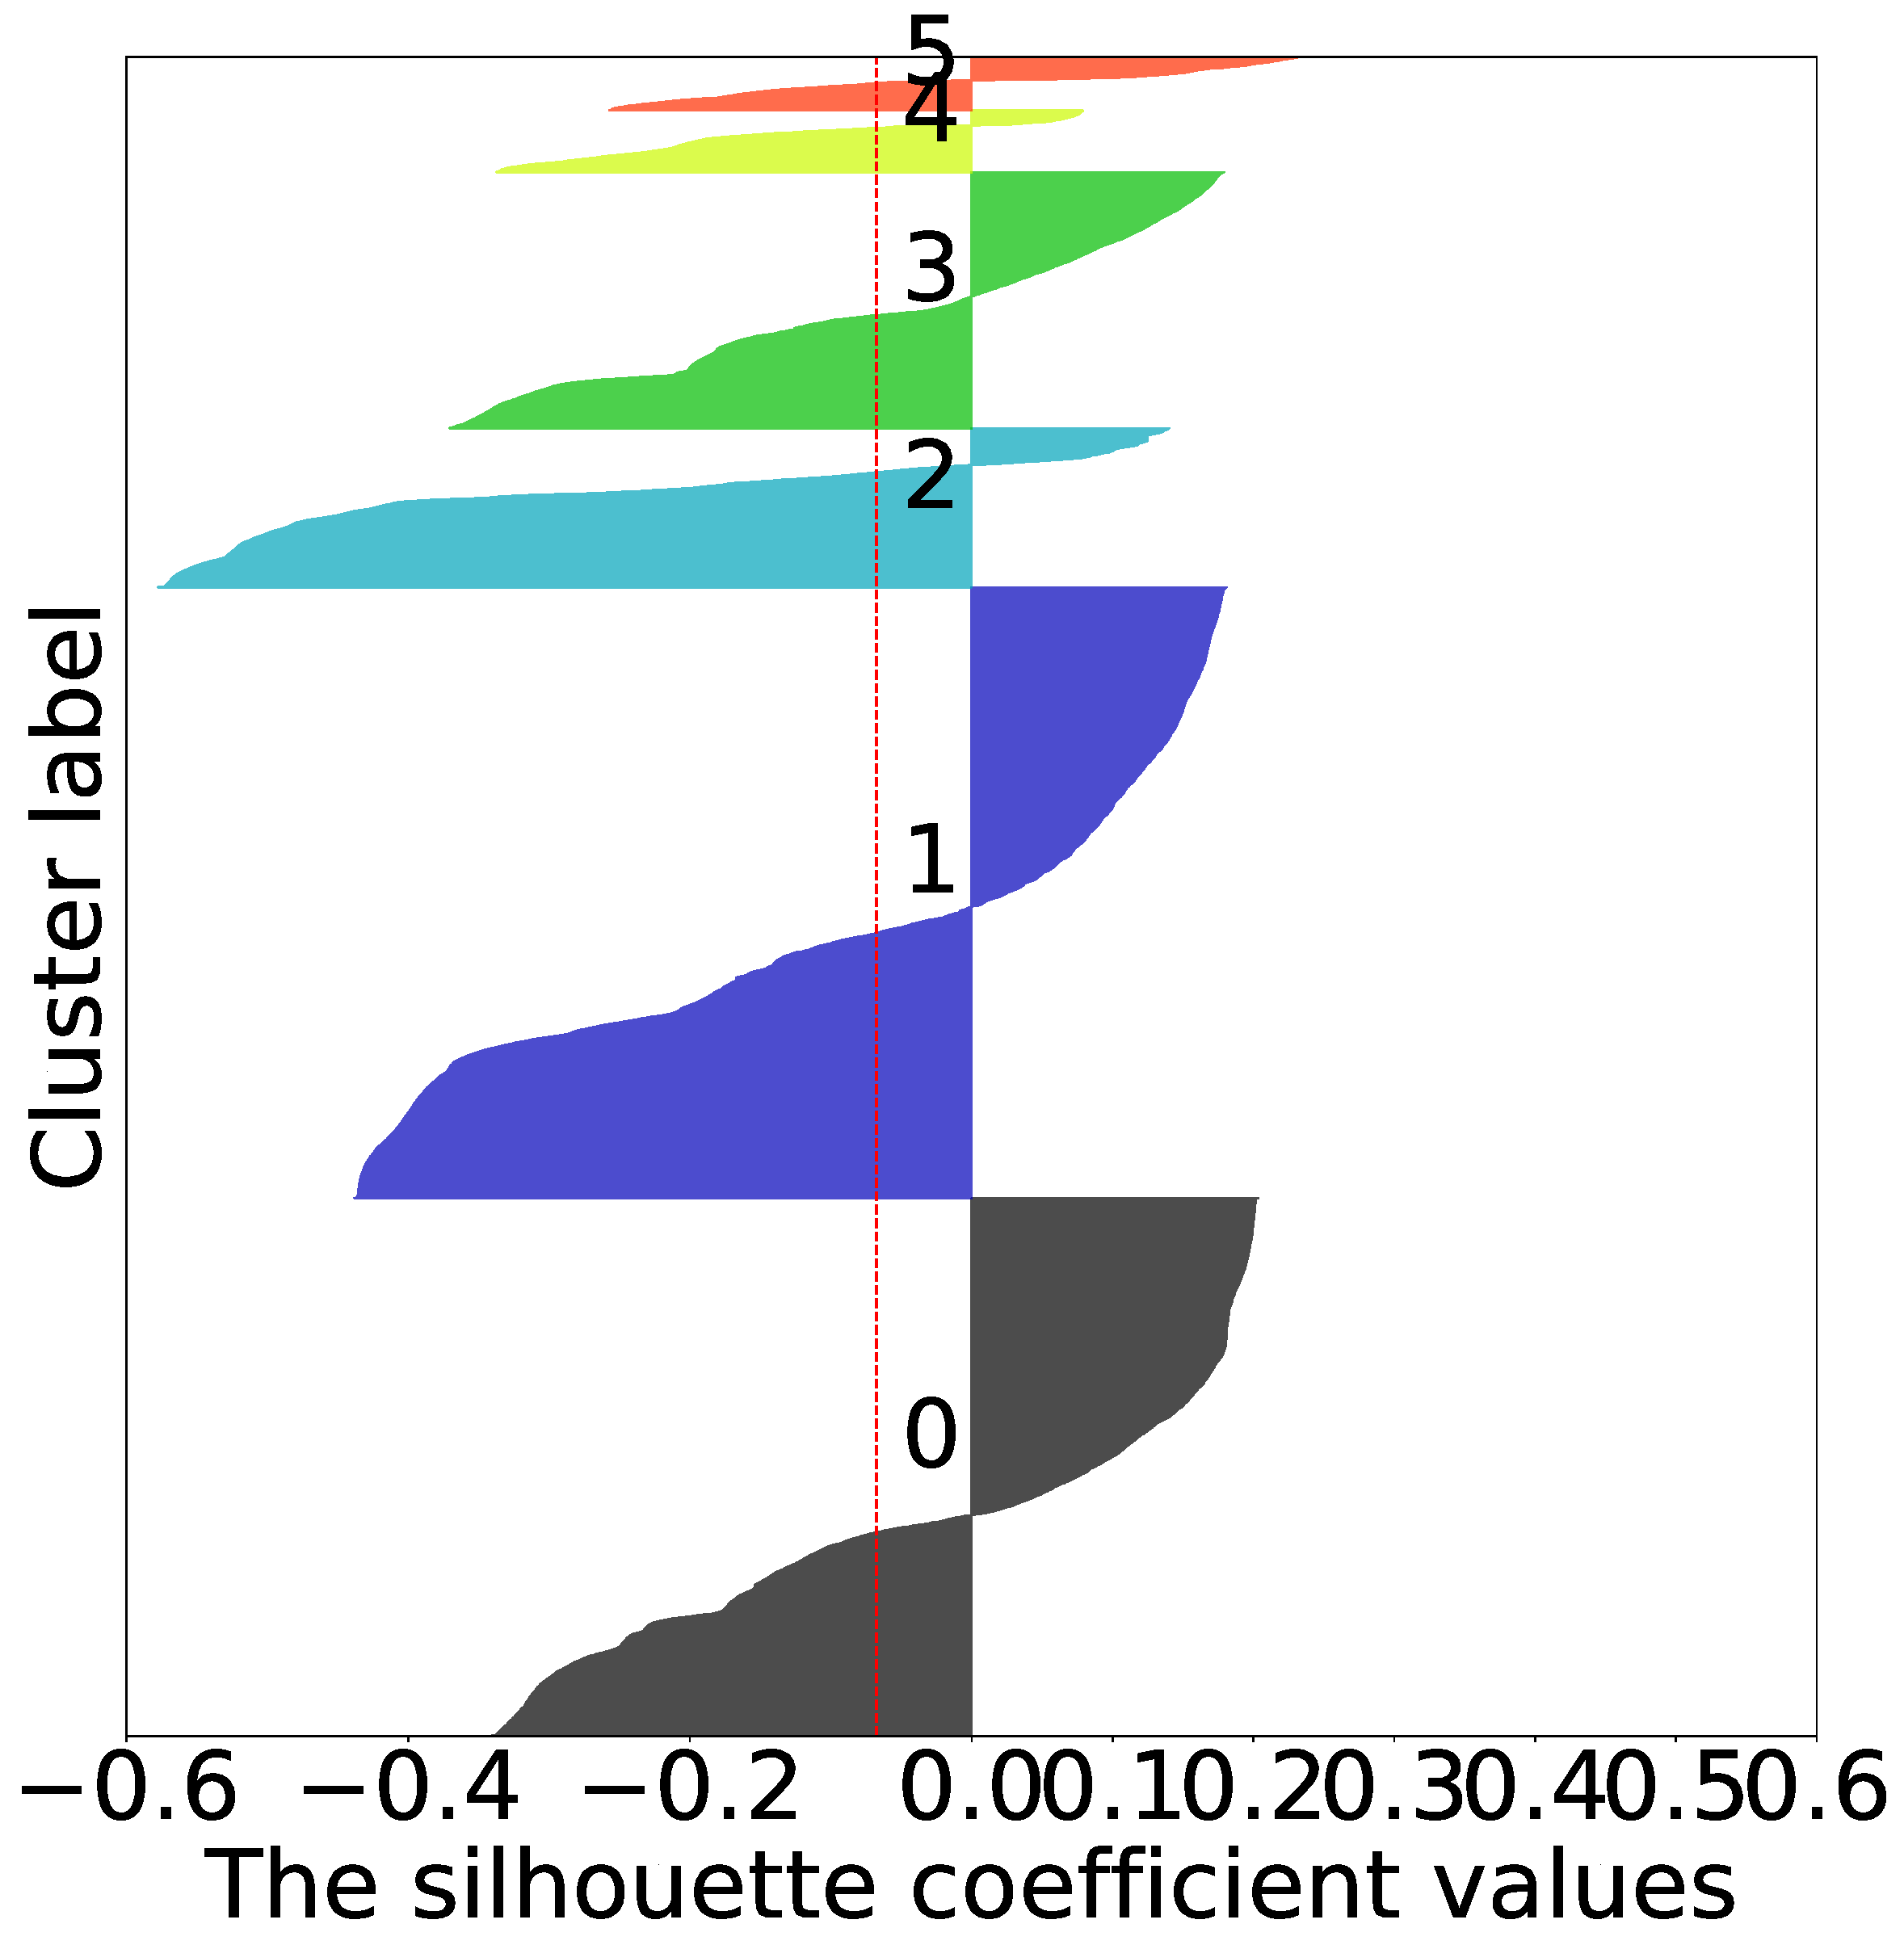
\includegraphics[width=0.33\textwidth]{figures/silhouette/silhouette_statistics_6.pdf}
    }
        \subfloat[n\_clusters = 7]{
        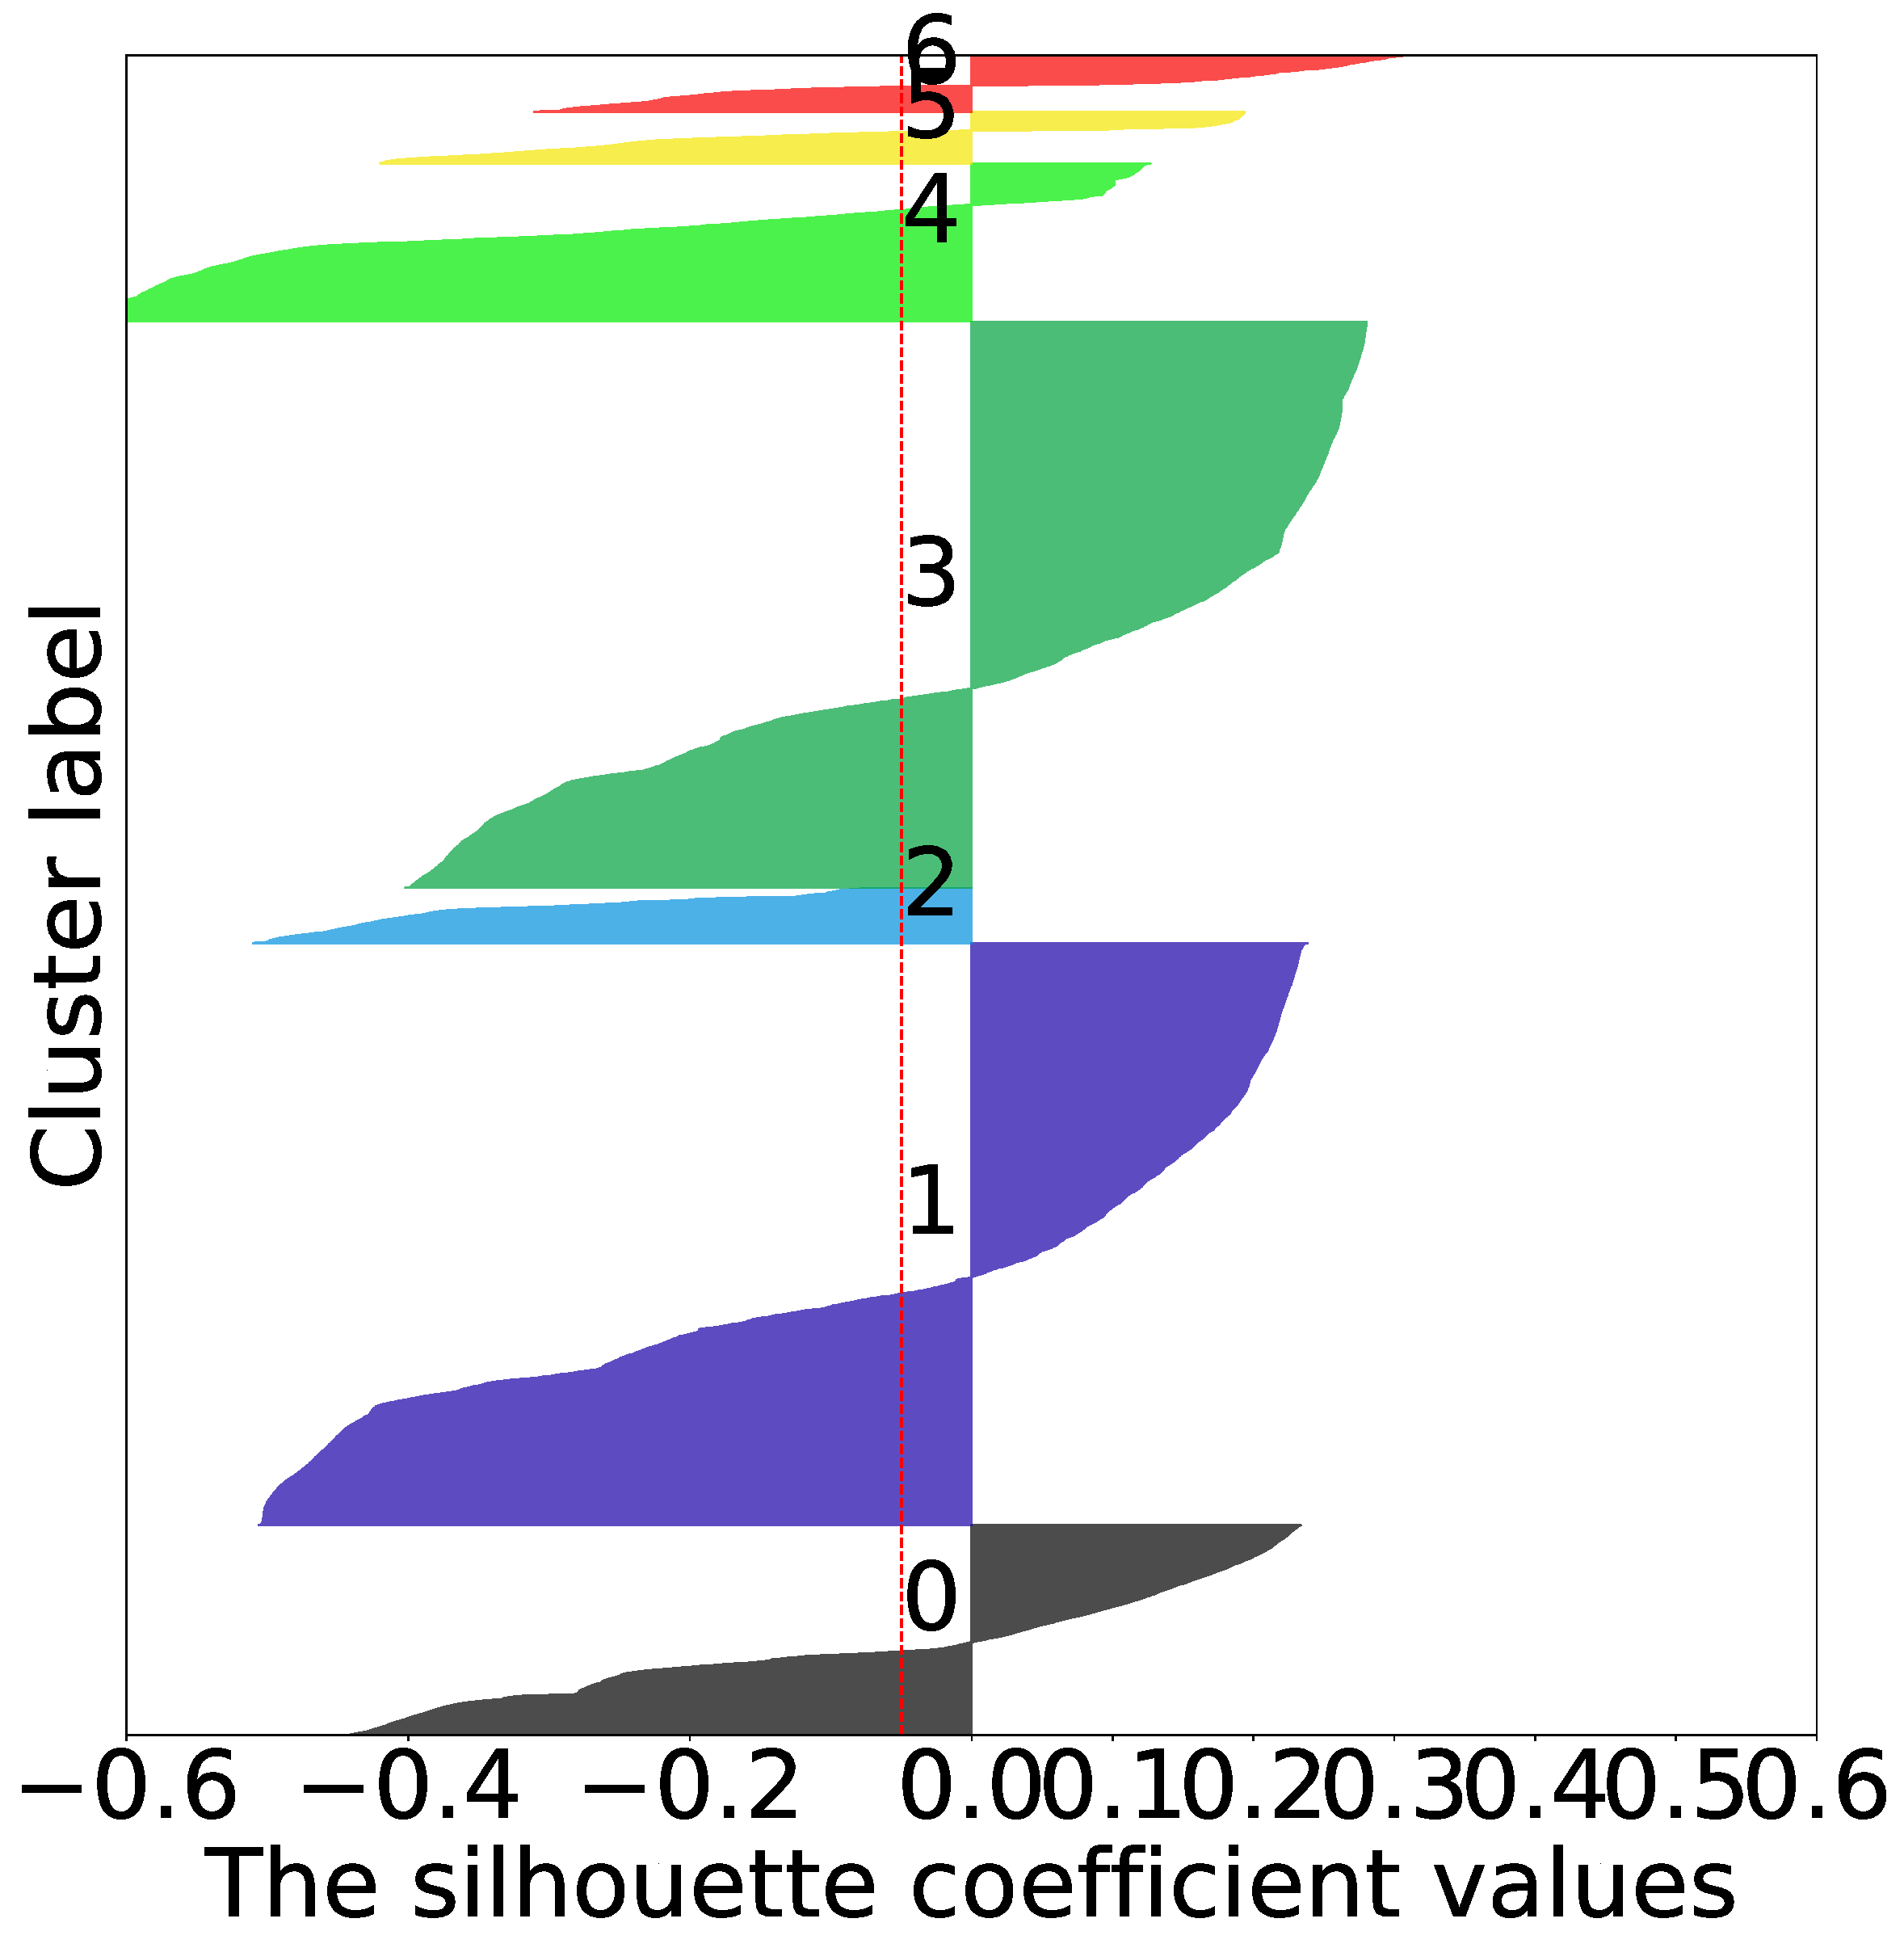
\includegraphics[width=0.33\textwidth]{figures/silhouette/silhouette_statistics_7.pdf}
    }
    \caption{Silhouette analysis for KMeans clustering on statistics analysis of windowed time-series data directly}
    \label{fig_silhouette_statistics}
\end{figure}

Ultimately, we used more descriptive statistics to help understand its central tendency, spread, and shape to aid alerting. We can use nine descriptive statistics metrics to provide valuable insights into the characteristics of the data: percentiles (25\%, 50\%, 75\%), kurtosis, maximum, minimum, skewness, standard deviation, and variance, as defined in Subsection \ref{subsec:statistics}.

The histogram distribution graph is shown in Figure \ref{fig_load_gpu_histogram}. The graph shows that kurtosis, mean, skewness, and standard deviation have a central tendency. We cannot find a good separation for these data, so these metrics cannot separate good and bad jobs. Combined with the analysis of the monitoring data in production and the actual need for job alerting, which is to find out the bad jobs that can be greatly improved, we eventually fine-tuned and discovered that 20 in the 75th percentile and 32 in the maximum are good separations, as defined in Algorithm \ref{algo:statistics}.

\begin{algorithm}[H]
\SetAlgoLined
\KwData{Array, Fixed-size sliding window of latest GPU usage history: $A$}
\KwResult{Boolean, indicating if an alert should be raised}
\SetKwFunction{FMain}{CheckAlert}
\SetKwFunction{FPercentile}{getPercentile}
\SetKwProg{Fn}{Function}{:}{}

\Fn{\FPercentile{$array$, $divide$}}{
    Sort $array$ in ascending order\;
    \Return $array[\lfloor(\text{len}(array) - 1) / divide\rfloor]$\;
}

\Fn{\FMain{$metrics$}}{
    $P_{75} \leftarrow \FPercentile(A, \frac{4}{3})$\;
    $M \leftarrow \FPercentile(A, 1.0)$\;
    \If{$P_{75} < 20$ \textbf{or} $M < 32$}{
        \Return true\;
    }
    \Else{
        \Return false\;
    }
}

\caption{Algorithm for checking GPU load alert based on percentile and maximum}
\label{algo:statistics}
\end{algorithm}

\begin{figure}[H]
    \centering
        \subfloat[25\%]{
        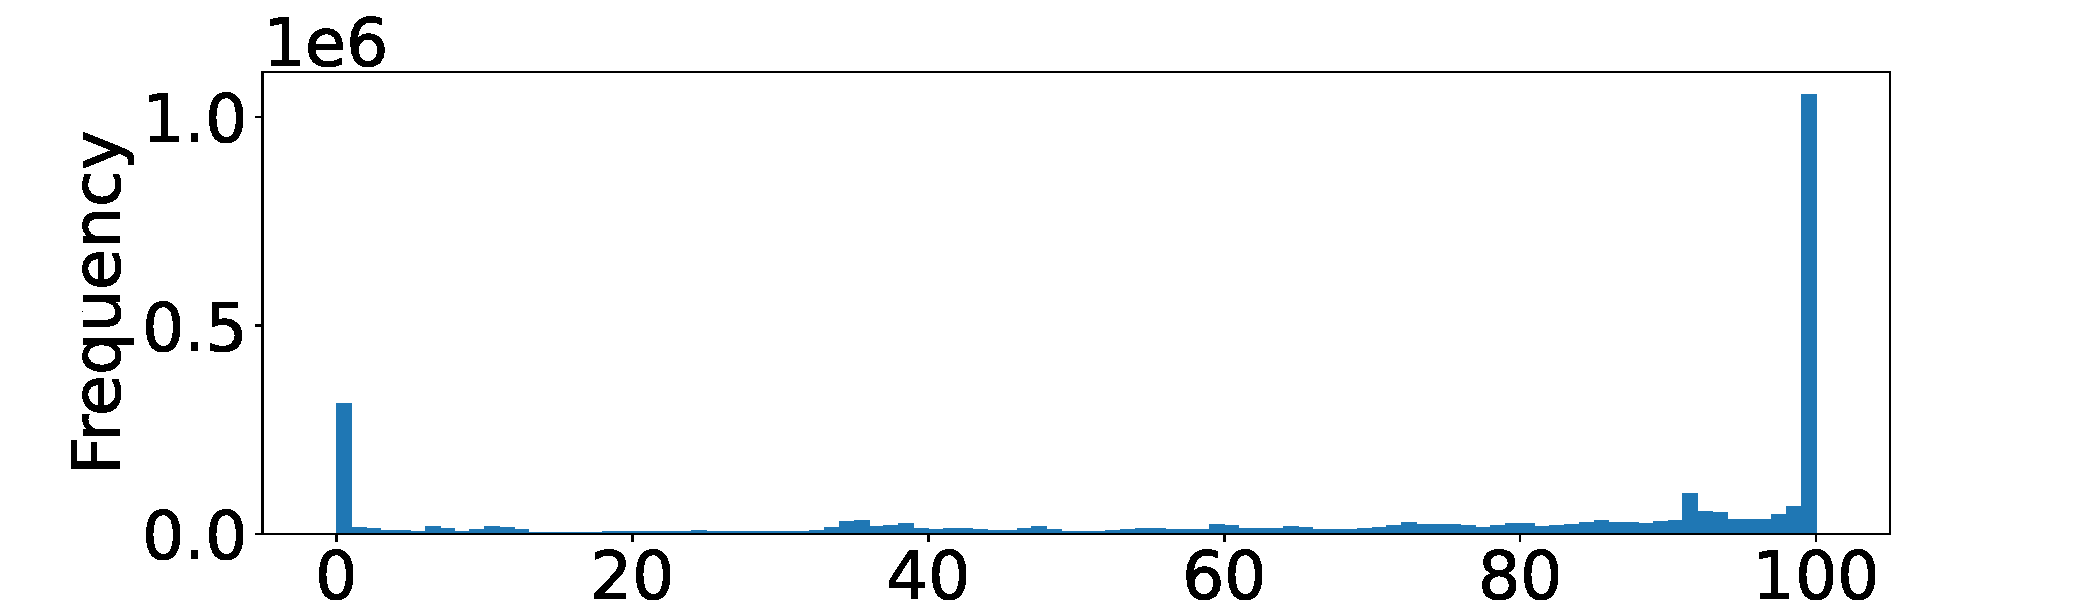
\includegraphics[width=0.5\textwidth]{figures/analysis/load_gpu_25_histogram.pdf}
    }
        \subfloat[50\%]{
        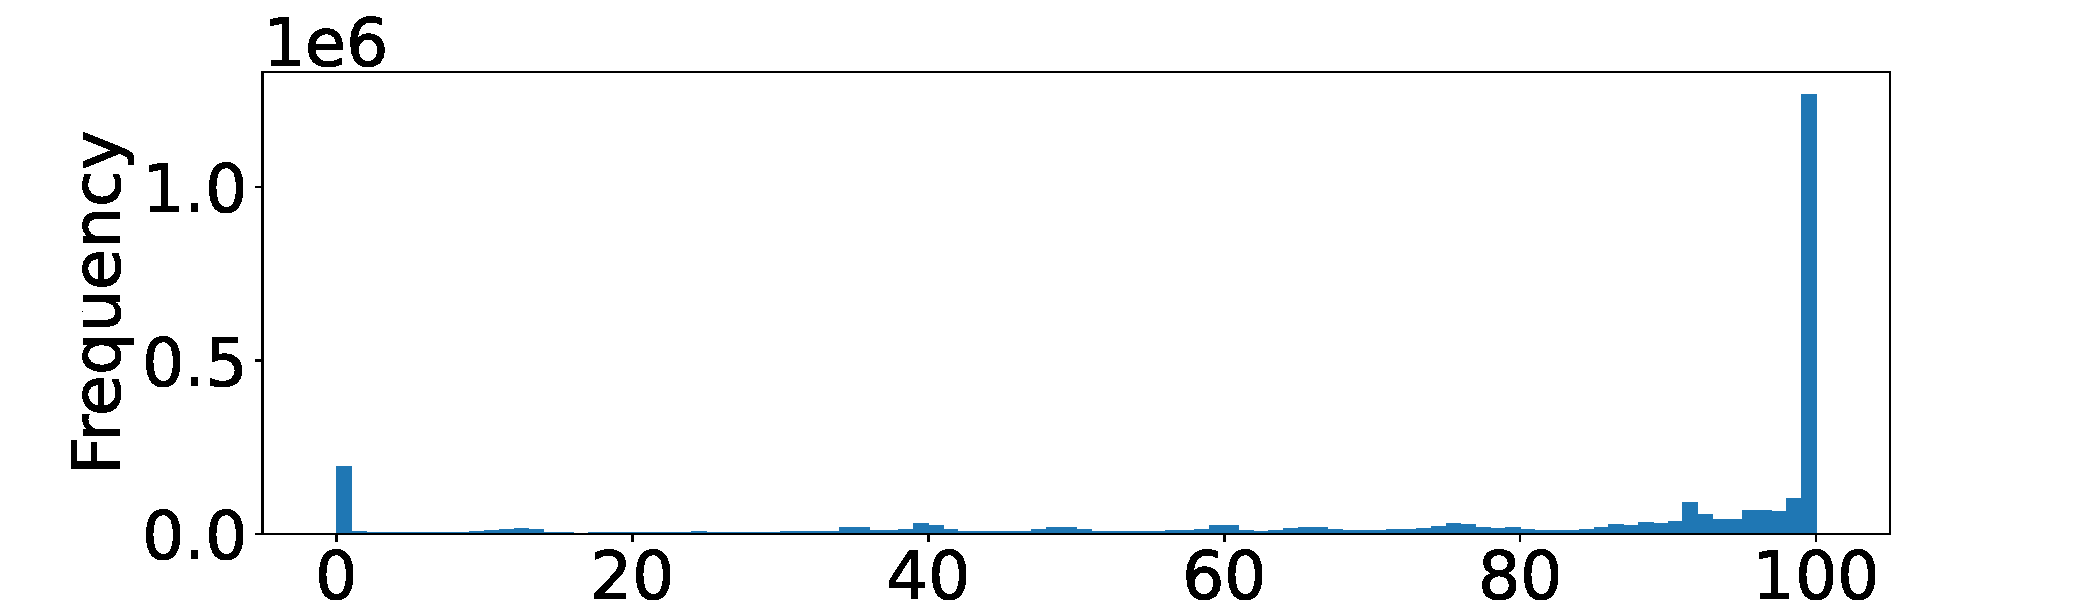
\includegraphics[width=0.5\textwidth]{figures/analysis/load_gpu_50_histogram.pdf}
    }\\
        \subfloat[75\%]{
        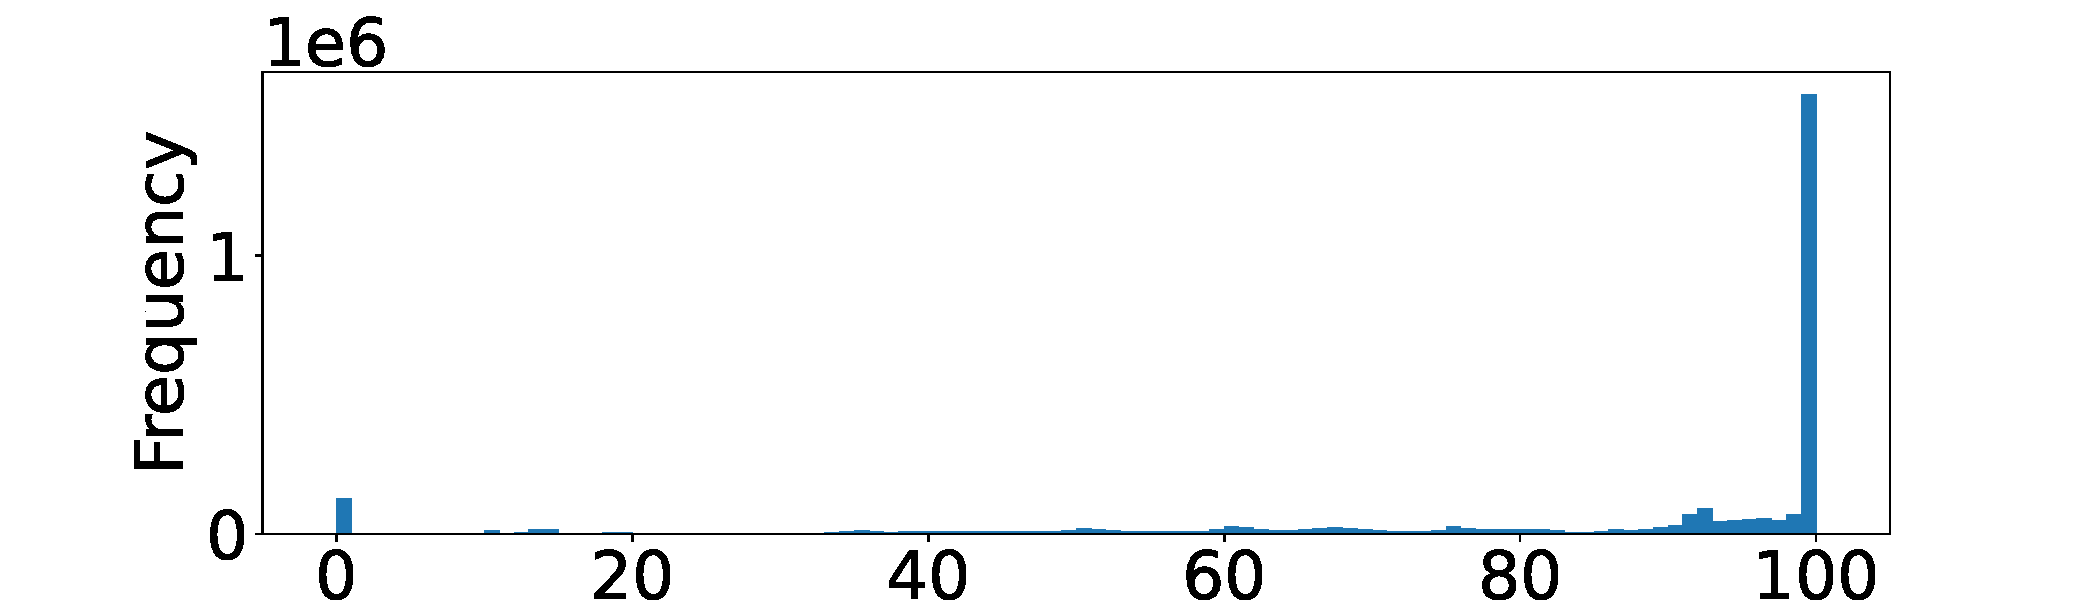
\includegraphics[width=0.5\textwidth]{figures/analysis/load_gpu_75_histogram.pdf}
    }
        \subfloat[Kurtosis]{
        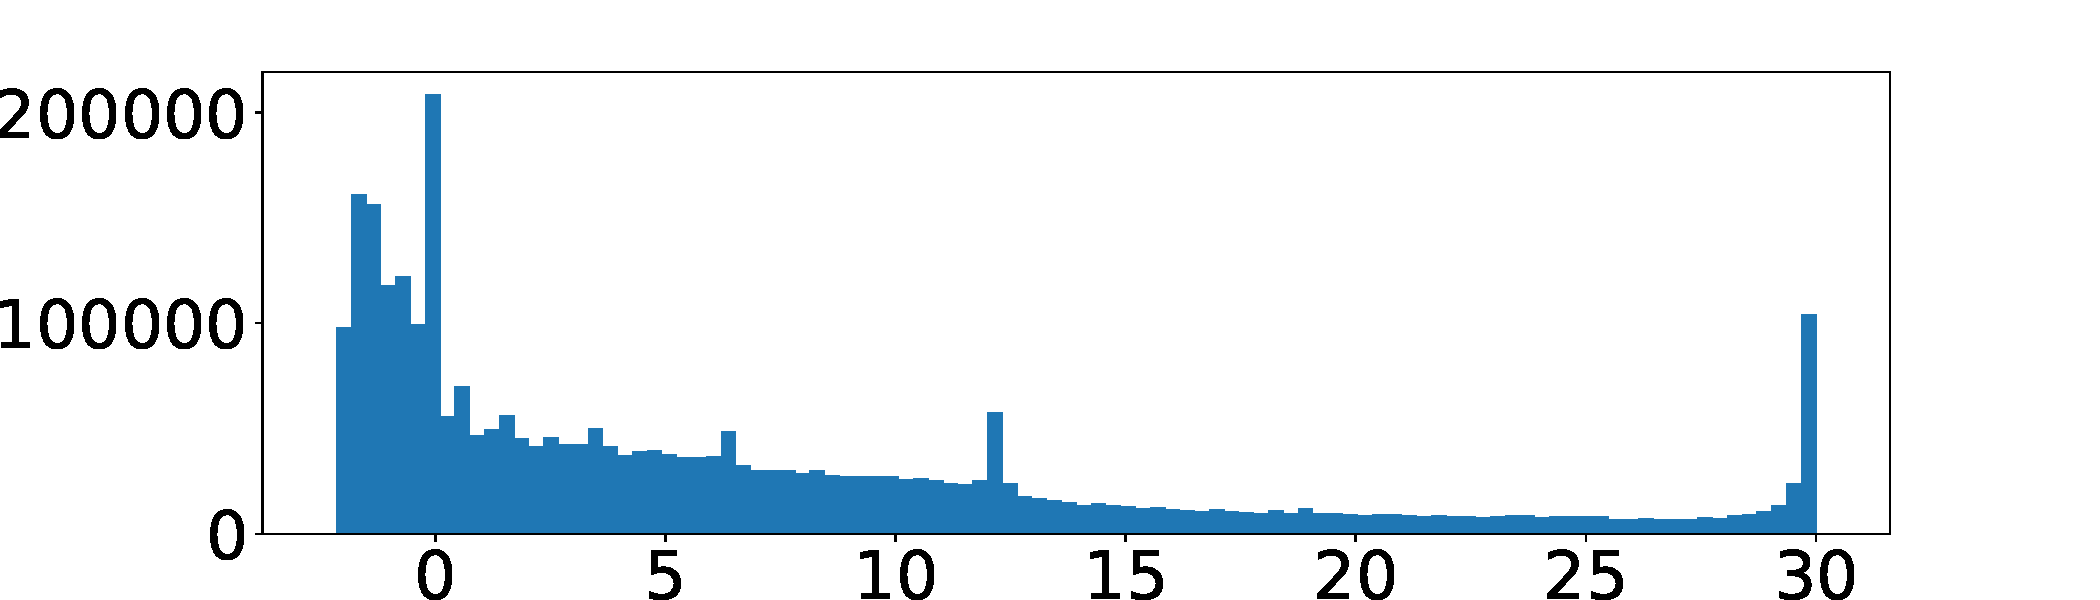
\includegraphics[width=0.5\textwidth]{figures/analysis/load_gpu_kurt_histogram.pdf}
    }\\
        \subfloat[Maximum]{
        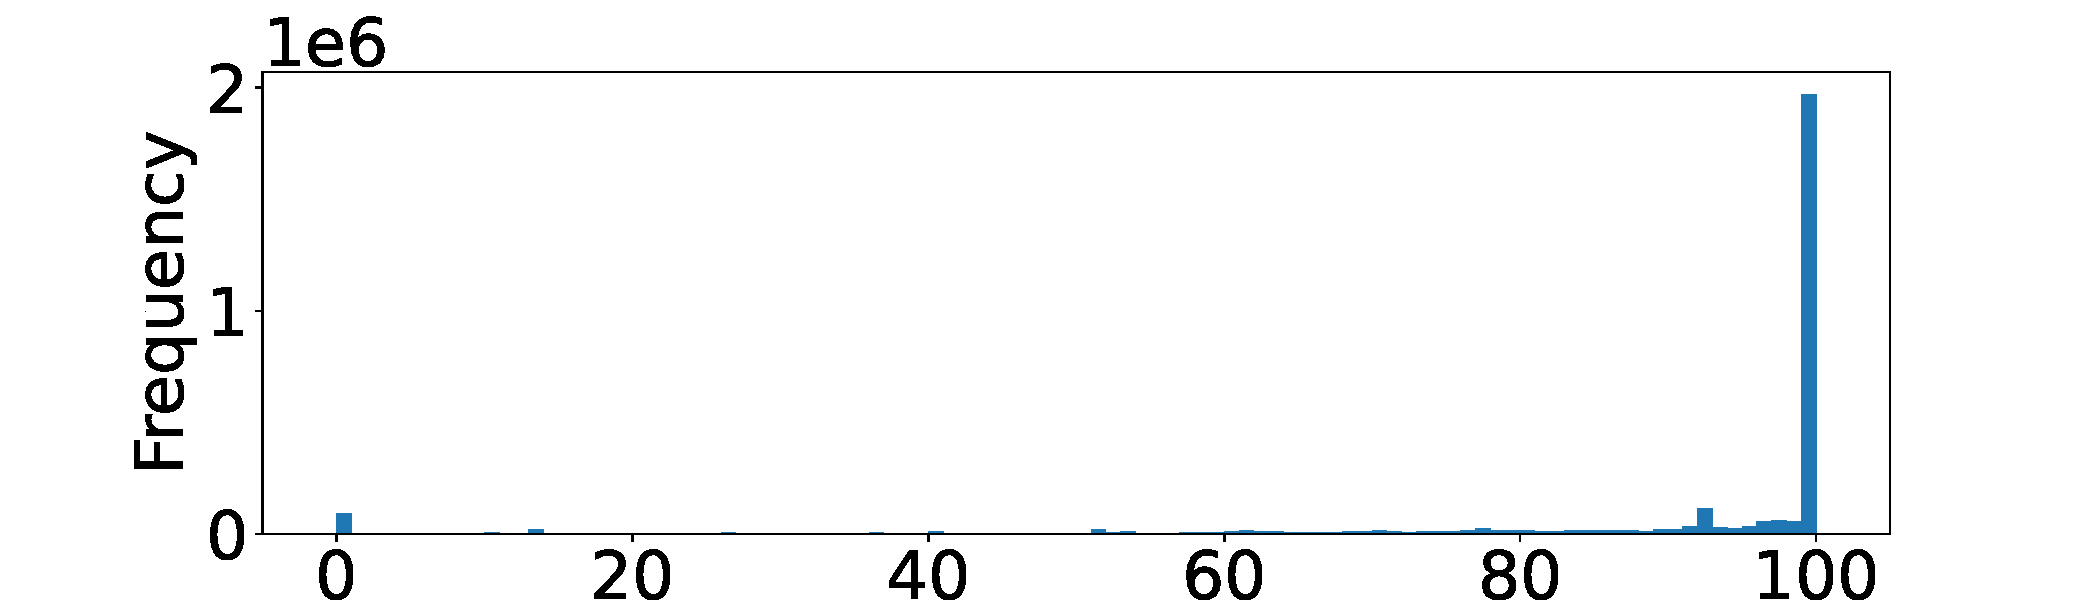
\includegraphics[width=0.5\textwidth]{figures/analysis/load_gpu_max_histogram.pdf}
    }
        \subfloat[Mean]{
        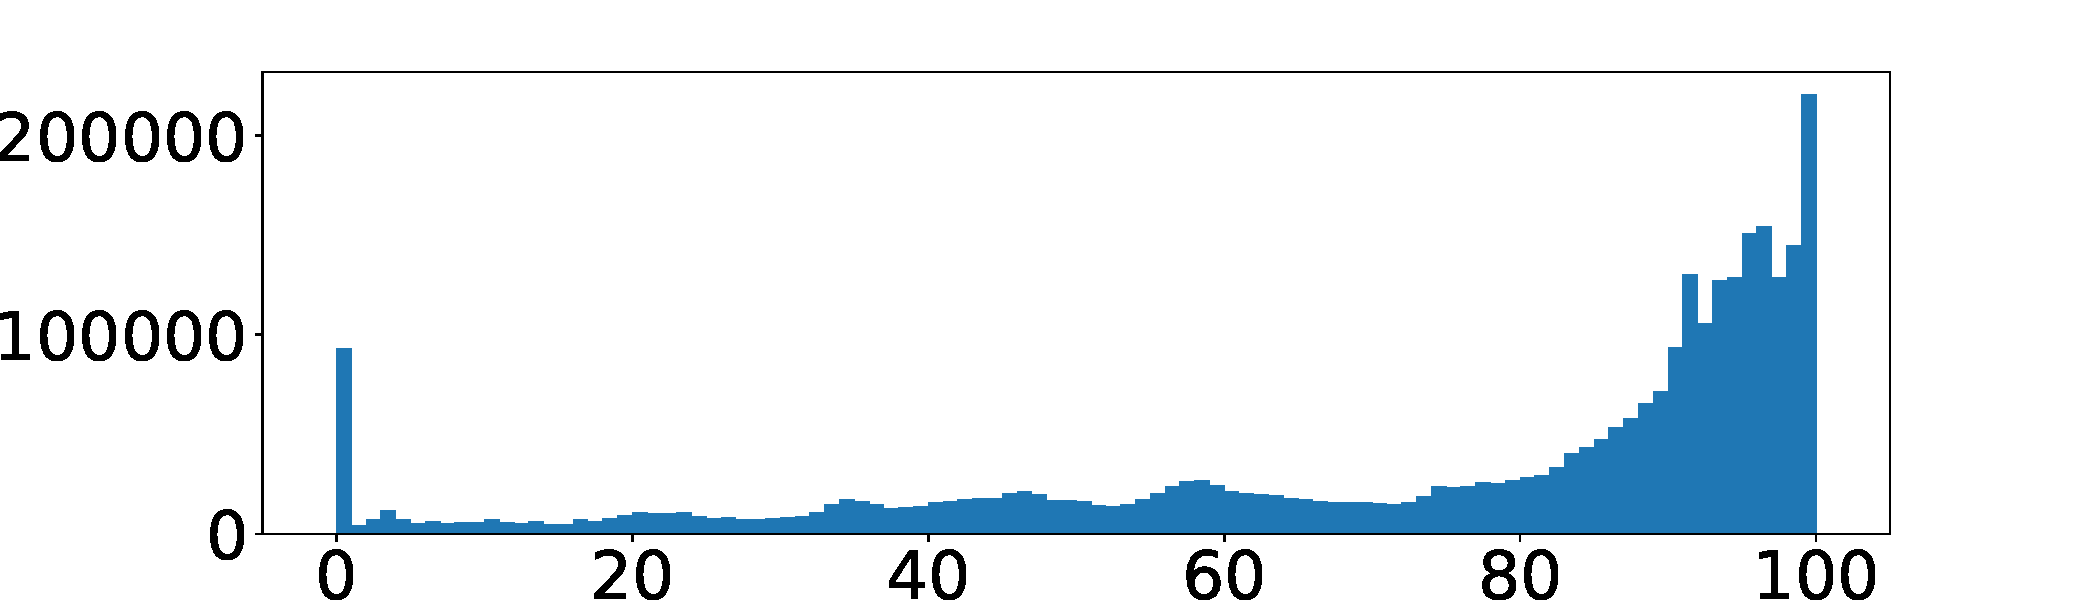
\includegraphics[width=0.5\textwidth]{figures/analysis/load_gpu_mean_histogram.pdf}
    }\\
        \subfloat[Minimum]{
        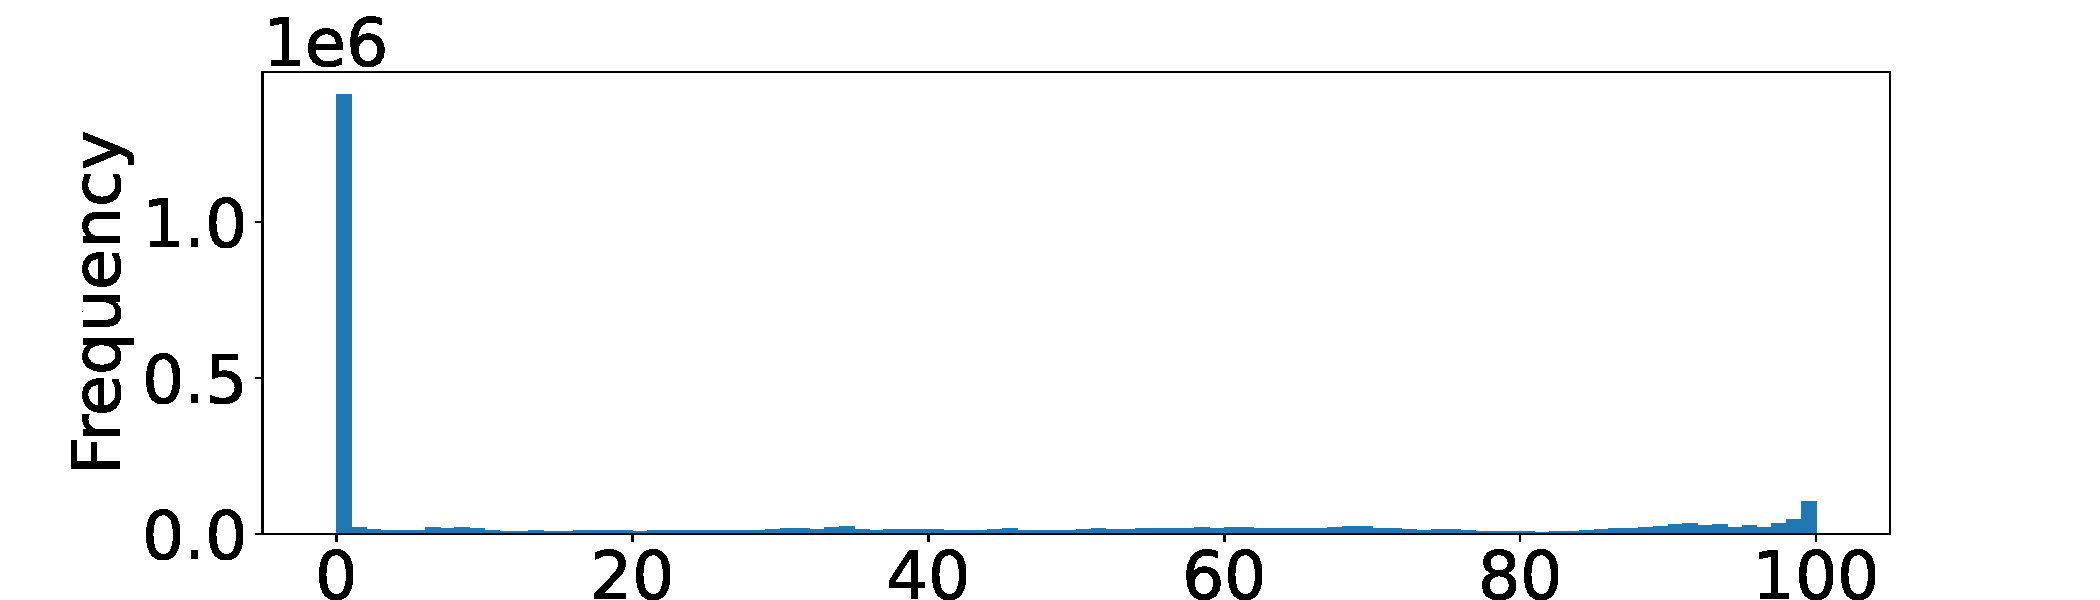
\includegraphics[width=0.5\textwidth]{figures/analysis/load_gpu_min_histogram.pdf}
    }
        \subfloat[Skewness]{
        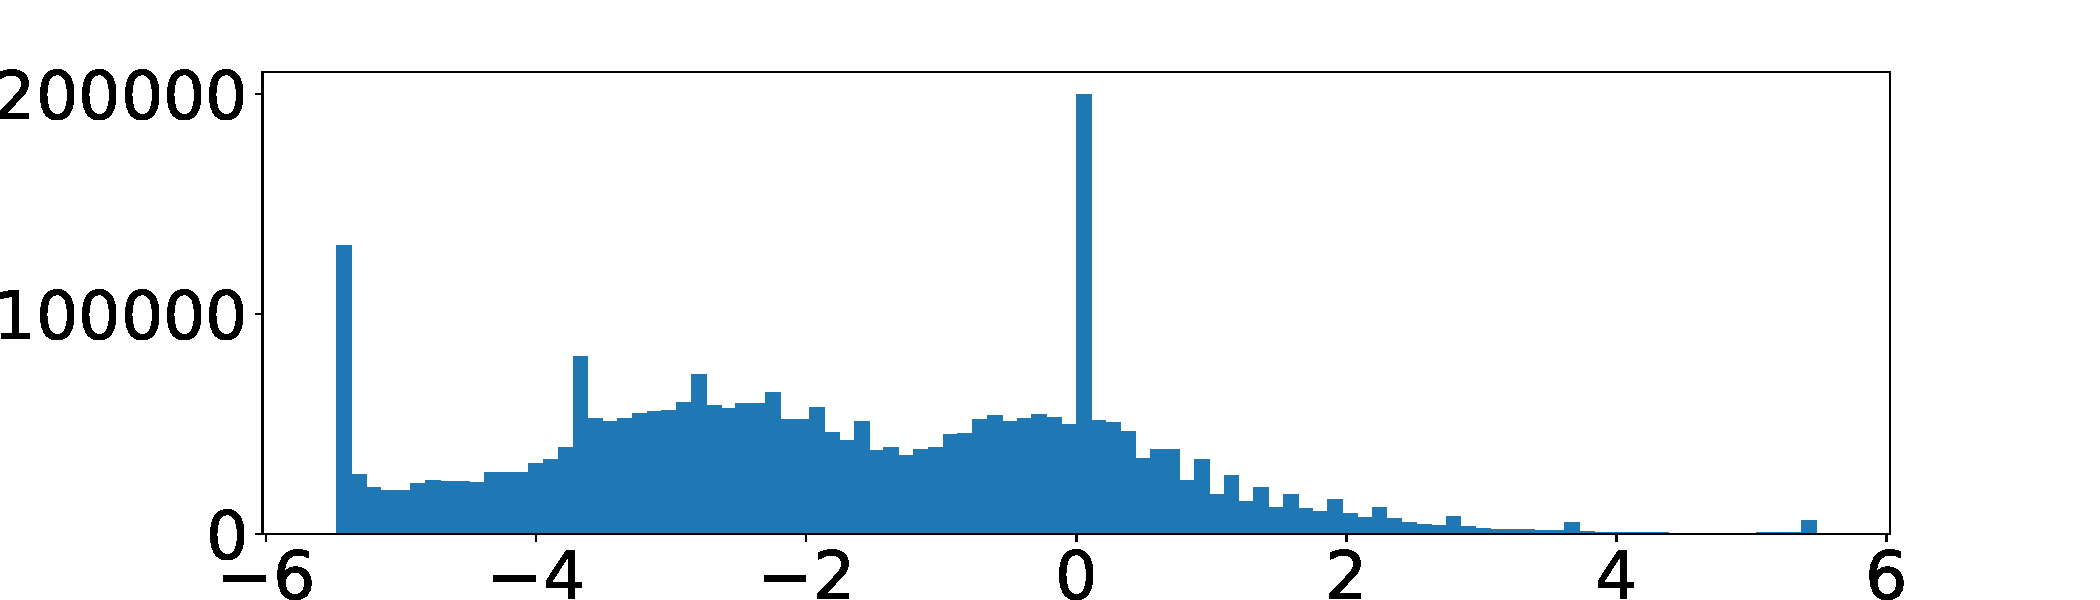
\includegraphics[width=0.5\textwidth]{figures/analysis/load_gpu_skew_histogram.pdf}
    }\\
        \subfloat[Standard deviation]{
        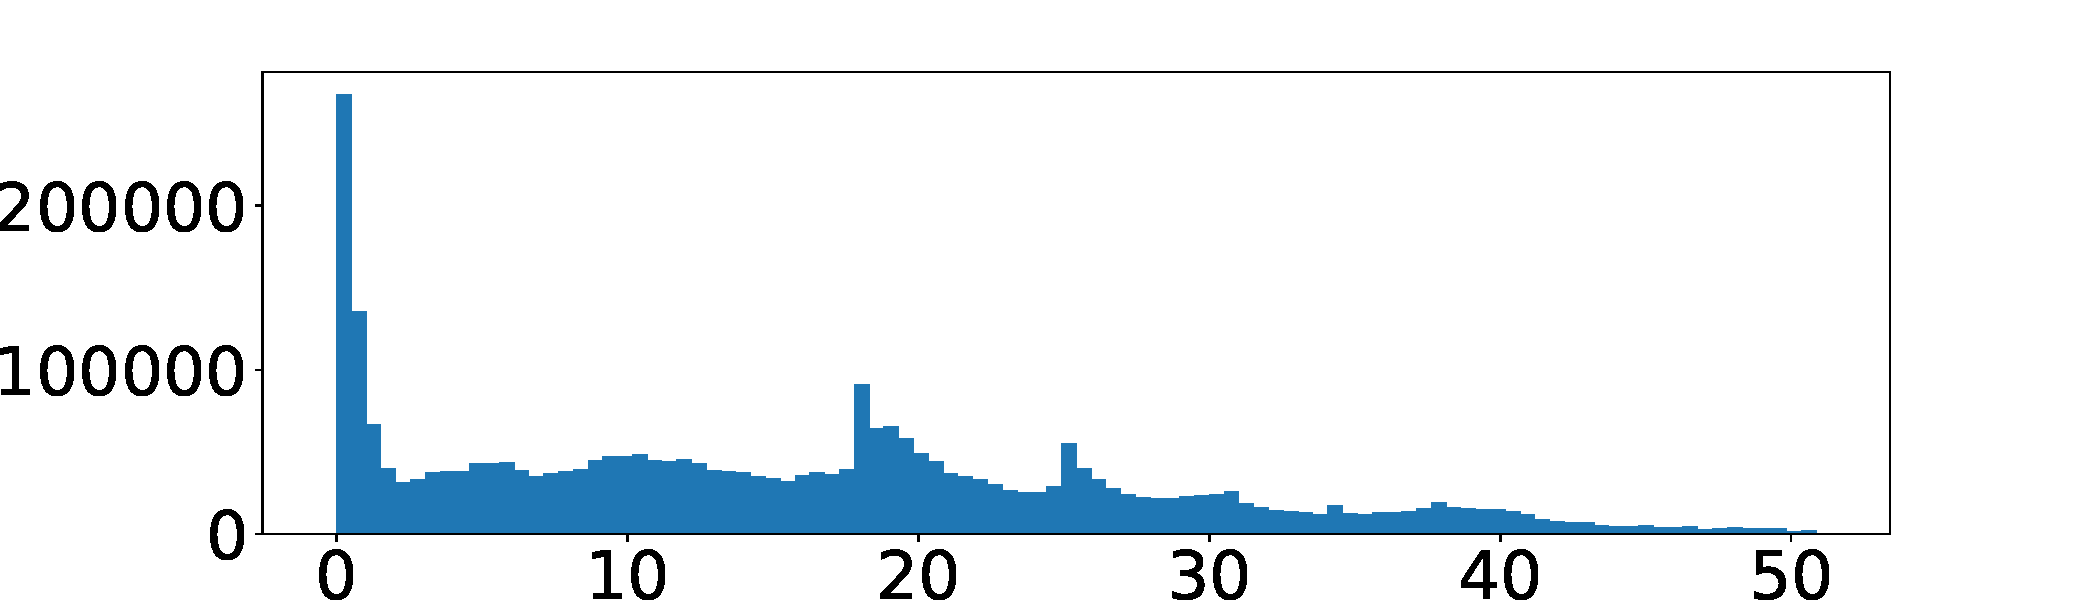
\includegraphics[width=0.5\textwidth]{figures/analysis/load_gpu_std_histogram.pdf}
    }
    \caption{Histogram of statistics analysis on windowed time-series load GPU data}
    \label{fig_load_gpu_histogram}
\end{figure}

\section{Alert service}
\label{sec:alertservice}
The alert service we implemented is built on the monitoring system. A good design is crucial for addressing all the research questions in Section \ref{sec:rqs}.

% communicates with the TimescaleDB through triggers to update the internal state in memory. 

Since message queues introduce a single point of failure, and can be challenging to debug, we decided not to use them. This increases the difficulty of our design, but aside from polling we do have an alternative: TimescaleDB, which is based on PostgreSQL. PostgreSQL has LISTEN and NOTIFY, so we can use triggers to execute NOTIFY after the insertion of each row, and Timescale Alert can LISTEN to the updates.

We also have continuous aggregates in TimescaleDB \cite{ConAggs}, Spark \cite{10.1145/2783258.2789993}, and Flink \cite{10.14778/3137765.3137777}, which can also be our choice.

As a result, we devised four solutions combining polling/triggers, and with or without continuous aggregates, to balance the \textbf{RQ1} and \textbf{RQ2} as mentioned in Section \ref{sec:rqs}.

\begin{itemize}
    \item \textbf{Polling with continuous aggregates}: Start/Stop polling as soon as job metadata updates. Use the continuous aggregates feature offered by TimescaleDB.

    \item \textbf{Polling with SQL aggregates}: Start/Stop polling as soon as job metadata updates, directly use SQL to do aggregates (without continuous aggregates and caching).

    \item \textbf{Triggers with continuous aggregates}: use the constant aggregates feature offered by TimescaleDB and query the aggregated result according to the information sent by the NOTIFY as soon as the message is received.

    \item \textbf{Triggers with in-memory aggregates}: Since our monitoring system can ensure that data arrives in order and has evenly distributed intervals, we can use a fixed-size container/ring (Circular Linked List) as the sliding window to store the history data, and do the aggregation by Golang. Here, we listen to the metrics data sent by the notification from the database and update the internal state in memory. % We dump the internal state by a fixed interval and send the dump to the user every time the user requests the current status over API.
\end{itemize}

Here is an empirical analysis of the four design choices mentioned above: We can choose either polling or triggers. With polling, the alert delay increases and will likely burden the database heavily with read operations. The alert delay is minimized with triggers, but we might slow down the database for writing operations.

We can also use the continuous aggregates in TimescaleDB. However, after investigation, we found they do not have sliding-window aggregation support with a high-level API. 

Since we want real-time alerts, we want to aggregate with a fixed-size sliding window that considers the latest data and drops the old data at any time, as shown in Figure \ref{fig_sliding_window}. However, TimescaleDB continuous aggregates, Spark, and Flink high-level API can only aggregate with a fixed start time, as shown in Figure \ref{fig_fixed_sliding_window}, which will work badly if we want to check the latest aggregation result at o'clock in this case since we will only have one data to aggregate in that window (only data at 11 o'clock as shown in the figure). Then, it is not very sensible to have an aggregation. Although the sliding window is not supported, we can overcome this issue by using a weighted average on the last two windows. However, it is still not a good candidate since triggers for continuous aggregates are not supported currently, as confirmed by the issue the author opened\footnote{https://github.com/timescale/timescaledb/issues/6500}. So we will have to burden the database by polling, which means many read operations plus many background jobs.

\begin{figure}[H]
    \centering
    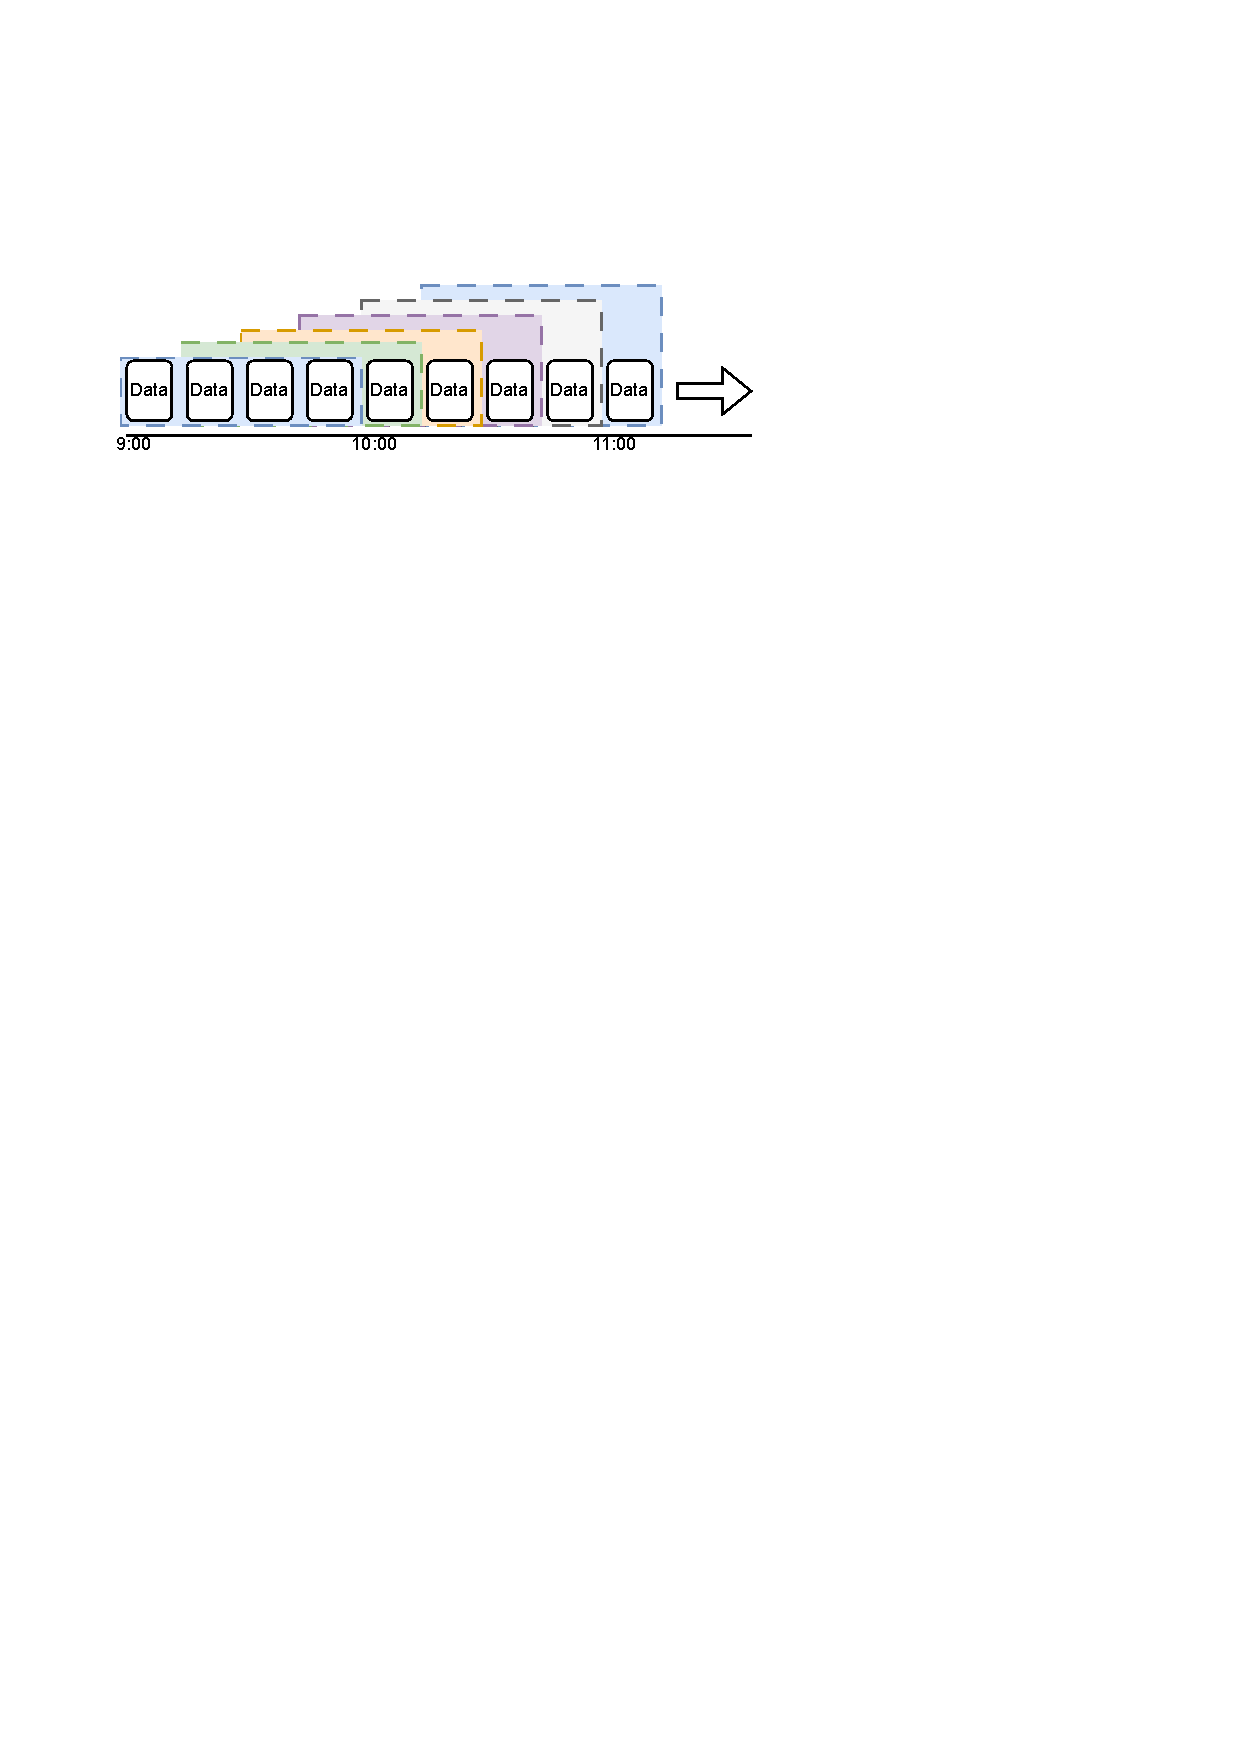
\includegraphics[width=1\textwidth]{figures/sliding-window.pdf}
    \caption{Sliding-window aggregation on the last 1 hour’s data}
    \label{fig_sliding_window}
\end{figure}

\begin{figure}[H]
    \centering
    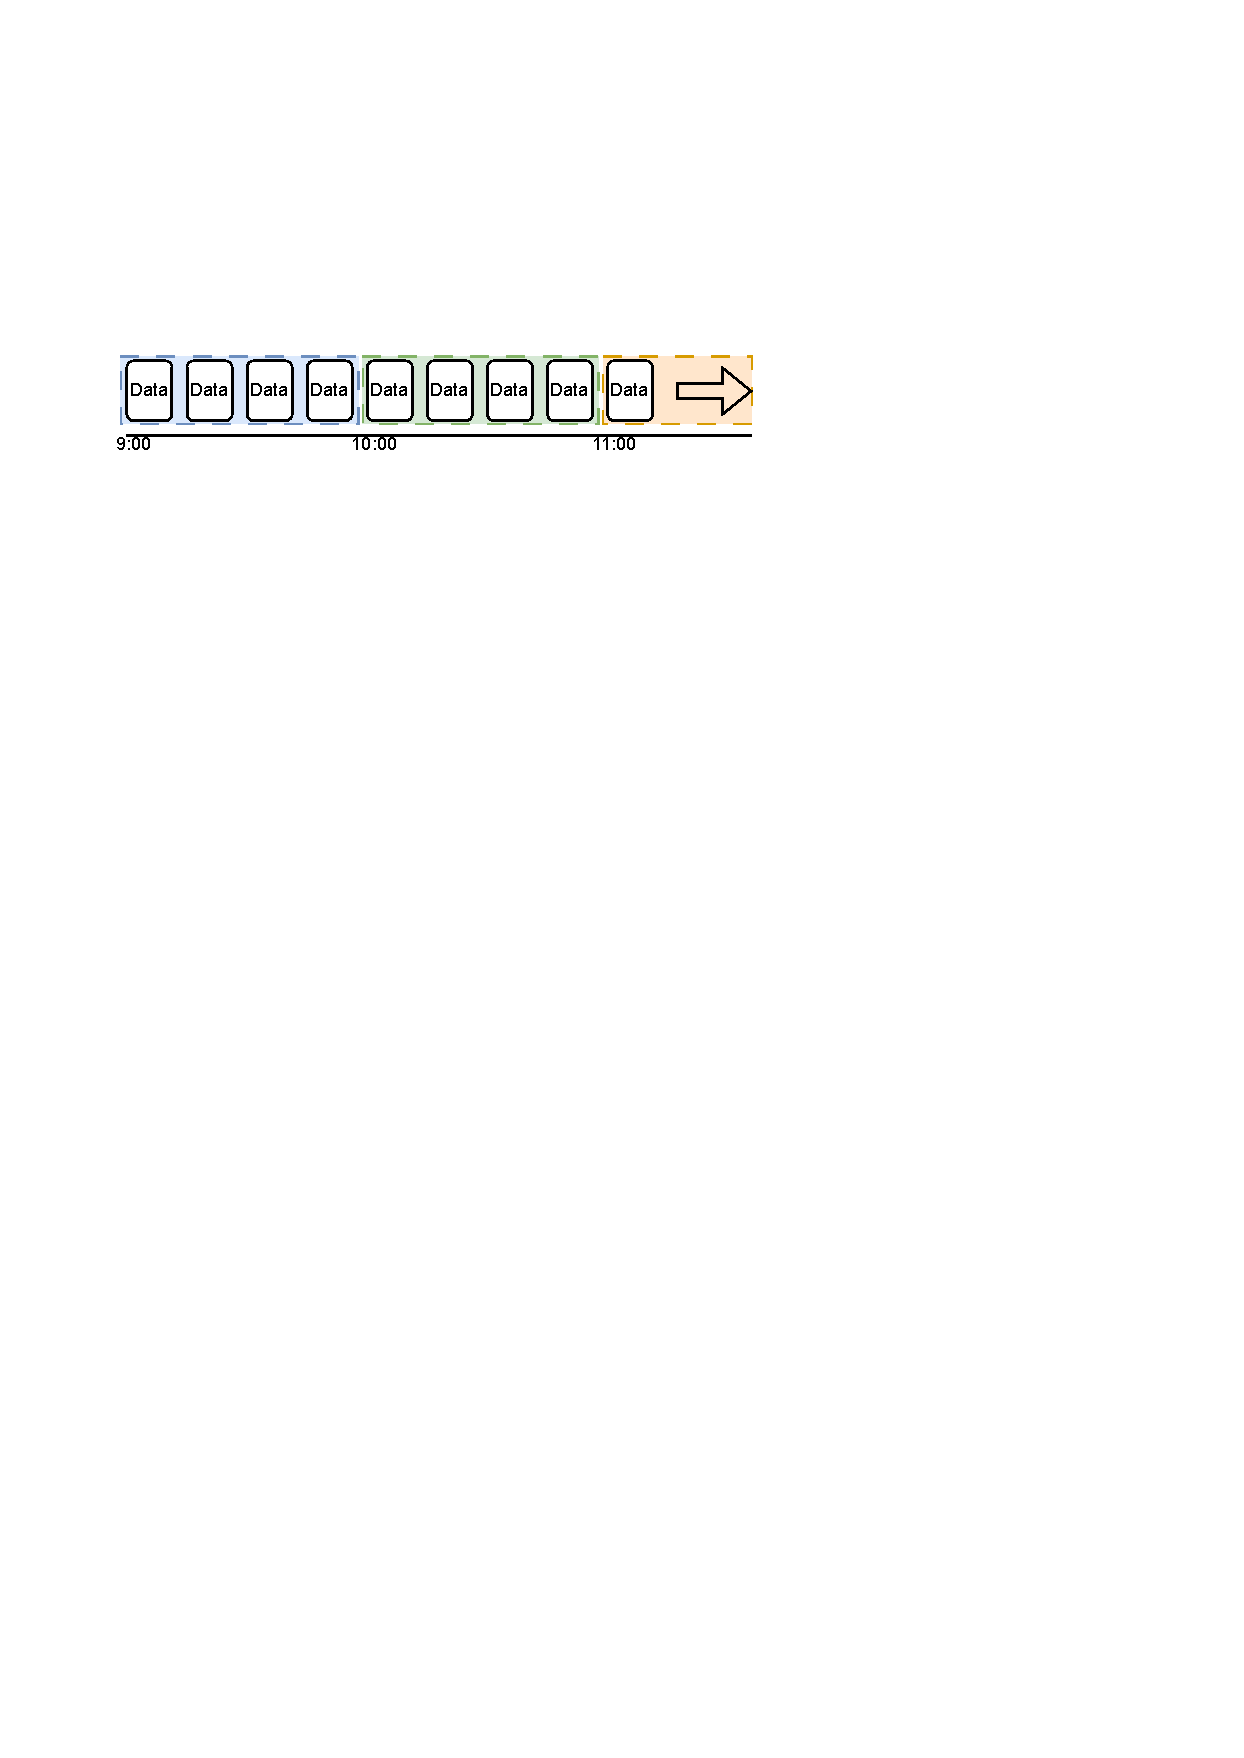
\includegraphics[width=1\textwidth]{figures/fixed-sliding-window.pdf}
    \caption{Aggregation with a fixed start time}
    \label{fig_fixed_sliding_window}
\end{figure}

We need to benchmark all 4 design choices to reach a final decision, which will be further discussed in SubSection \ref{subsec:performance}. Here are other specifications for the alert services:

The alert service can create or destroy the internal state for specific jobs by listening to job metadata updates generated by the database triggers. Whenever we have a new alert or the alert is dismissed, we write the event into logs. We garbage collect stale jobs to avoid memory leaks. We get the aggregation result as soon as data are inserted. For the dashboard RESTful API integration, handling the one-writer, multiple-reader problem can be very complex if we directly let the API server access our internal state, as starvation can quickly happen, and thus cause significantly reduced performance. In the end, we chose to convert the issue into the one-writer, one-reader problem by dumping the alert state with a thread separately at regular intervals into the JSON string, so that we can easily tackle the issue by simply using the thread-safe map and mutual exclusion lock, thus resolving \textbf{RQ3} in Section \ref{sec:rqs}.

% The triggers with an in-memory aggregates approach leverage in-memory processing capabilities to analyze GPU metrics in real-time. This involves maintaining an in-memory cache of aggregated metrics and facilitating rapid alerting based on live data without continuous queries to the time-series database. The in-memory cache balances real-time responsiveness and resource efficiency in the alerting system.


The API design of the Timescale Alert to provide the data for other services is as follows:

\begin{itemize}
    \item \textbf{/version}: Same as Timescale Ingest, it displays the version information and build time.
    \item \textbf{/healthStatus}: Checking connection status between the timescale ingest and the database.
    \item \textbf{/dismiss/:host/:job/:gpu}: Disable or enable the alert for the specified GPU on the host from a specific job ID.
    \item \textbf{/history}: Displaying a list of JSON objects or a table that shows the alert history. It can be filtered by the host, username, job ID, and type.
    \item \textbf{/}: Displaying the current alert status that host, username, and job ID can also filter.
\end{itemize}

Below is an example showing the GPU alert history output section of the \texttt{seff} command. The alert information is printed via the above-mentioned \texttt{/history} endpoint. Here, there are a few alert histories related to the GPU usage. Each entry shows the time when the alert happened, the hostname, and the GPU ID that generated the alert event. It also shows the 75th percentile aggregation result for the sliding window time frame that contributes to the alert status change, and the \texttt{Normal} column shows whether this entry generates a new alert (with \texttt{x}) or clears the old alert (with \texttt{v}).

\begin{lstlisting}
$ seff 5465
GPU Alert History
-------------------------------------------------------------------
GPU Usage
                     Time   Hostname   GPU Id   75% (%)   Normal
2024-04-25T17:05:55+03:00     r14g04        2        5      x
2024-04-25T17:06:41+03:00     r14g04        2       21      v
2024-04-25T17:10:49+03:00     r14g05        1        8      x
2024-04-25T17:11:17+03:00     r14g05        1       23      v
-------------------------------------------------------------------
\end{lstlisting}

\section{Alert dashboard}

The alert dashboard reads data to display, to learn about the current job status. It renders tables through the web page to internal users, such as CSC user support experts. As shown in Figure \ref{fig_status_dashboard}, the dashboard has a counter for the viewers to know the total number of GPUs in use, and how many are currently on alert. Aside from sorting the data, the dashboard also allows the viewers to filter the data by job ID, user name, hostname, and alert status, so that viewers can quickly target different entities in question. In addition, the dashboard allows users to disable or re-enable job alerts, so that admins can improve the alert manually and focus more on those jobs, that have not been checked or can be improved.

\begin{figure}[H]
    \centering
    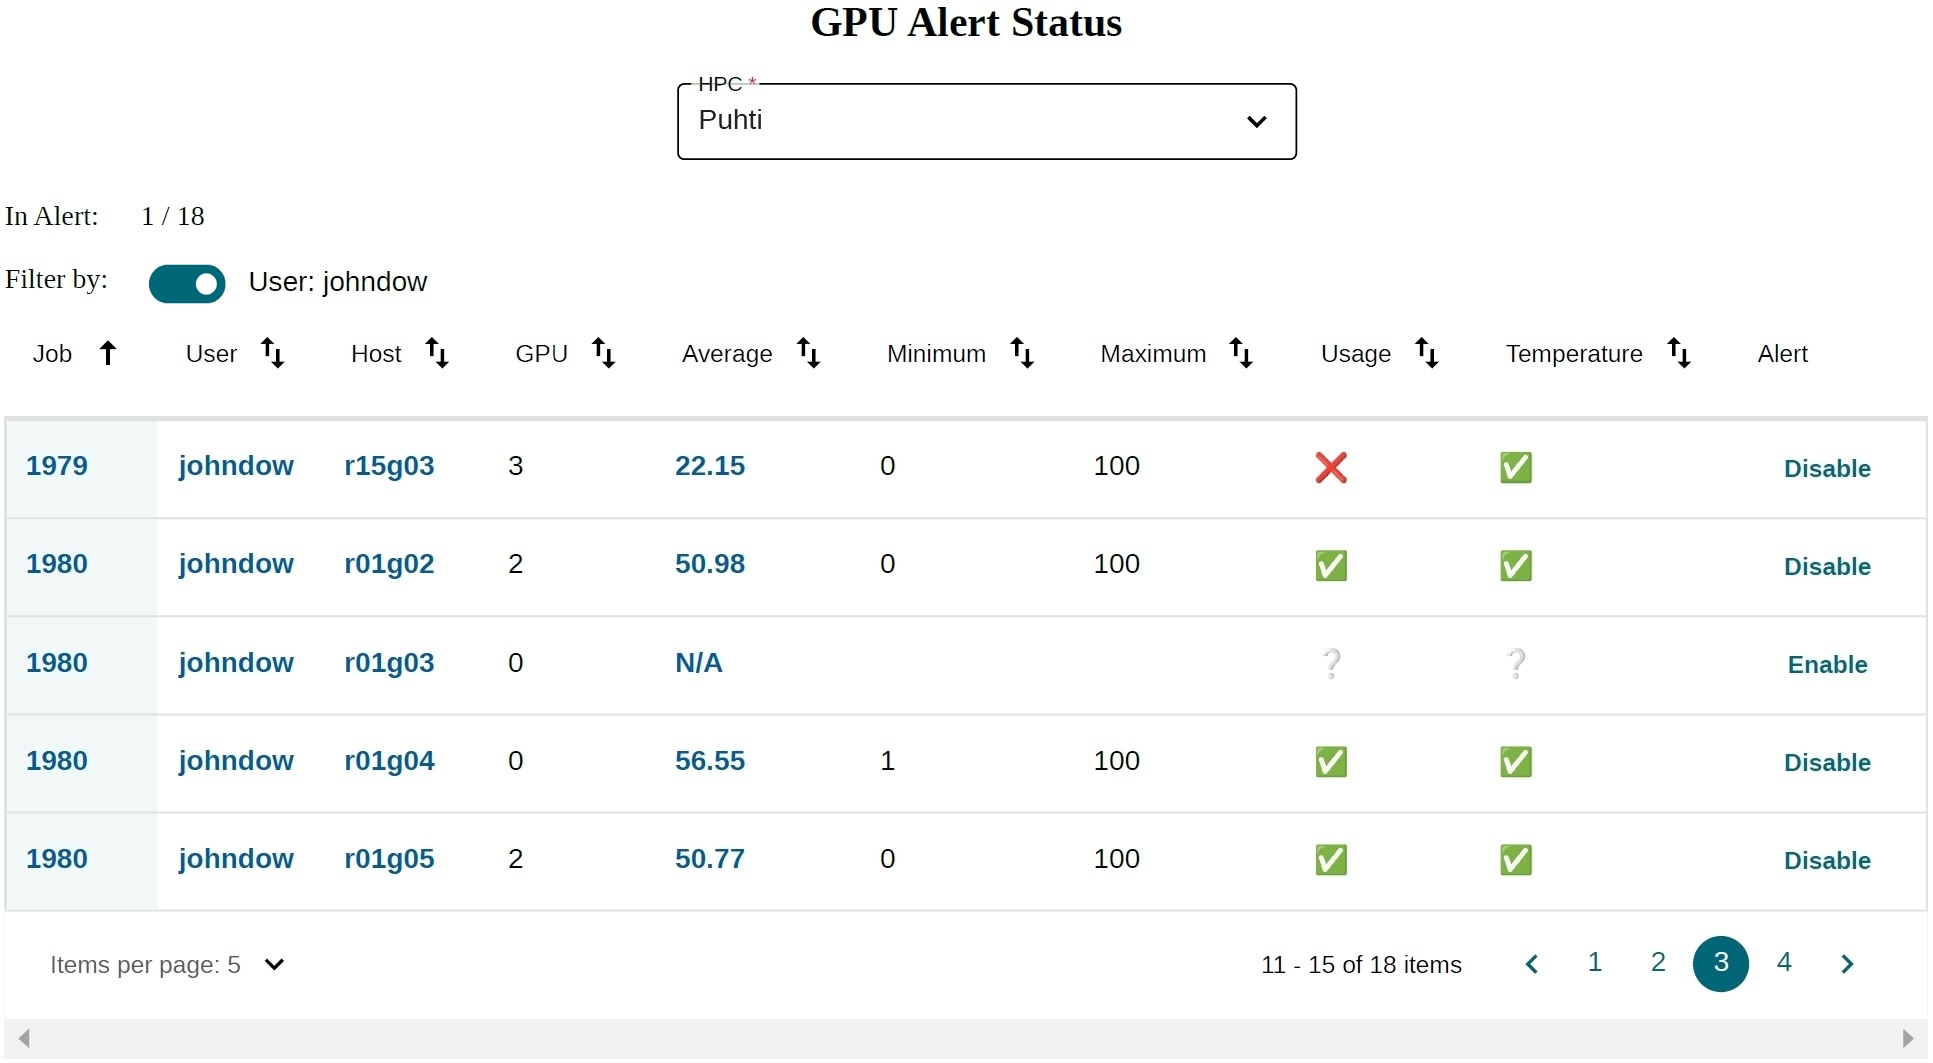
\includegraphics[width=1\textwidth]{figures/status-dashboard.jpeg}
    \caption{GPU alert status dashboard}
    \label{fig_status_dashboard}
\end{figure}

We also have a dashboard showing the alert history, as presented in Figure \ref{fig_history_dashboard}.

\begin{figure}[H]
    \centering
    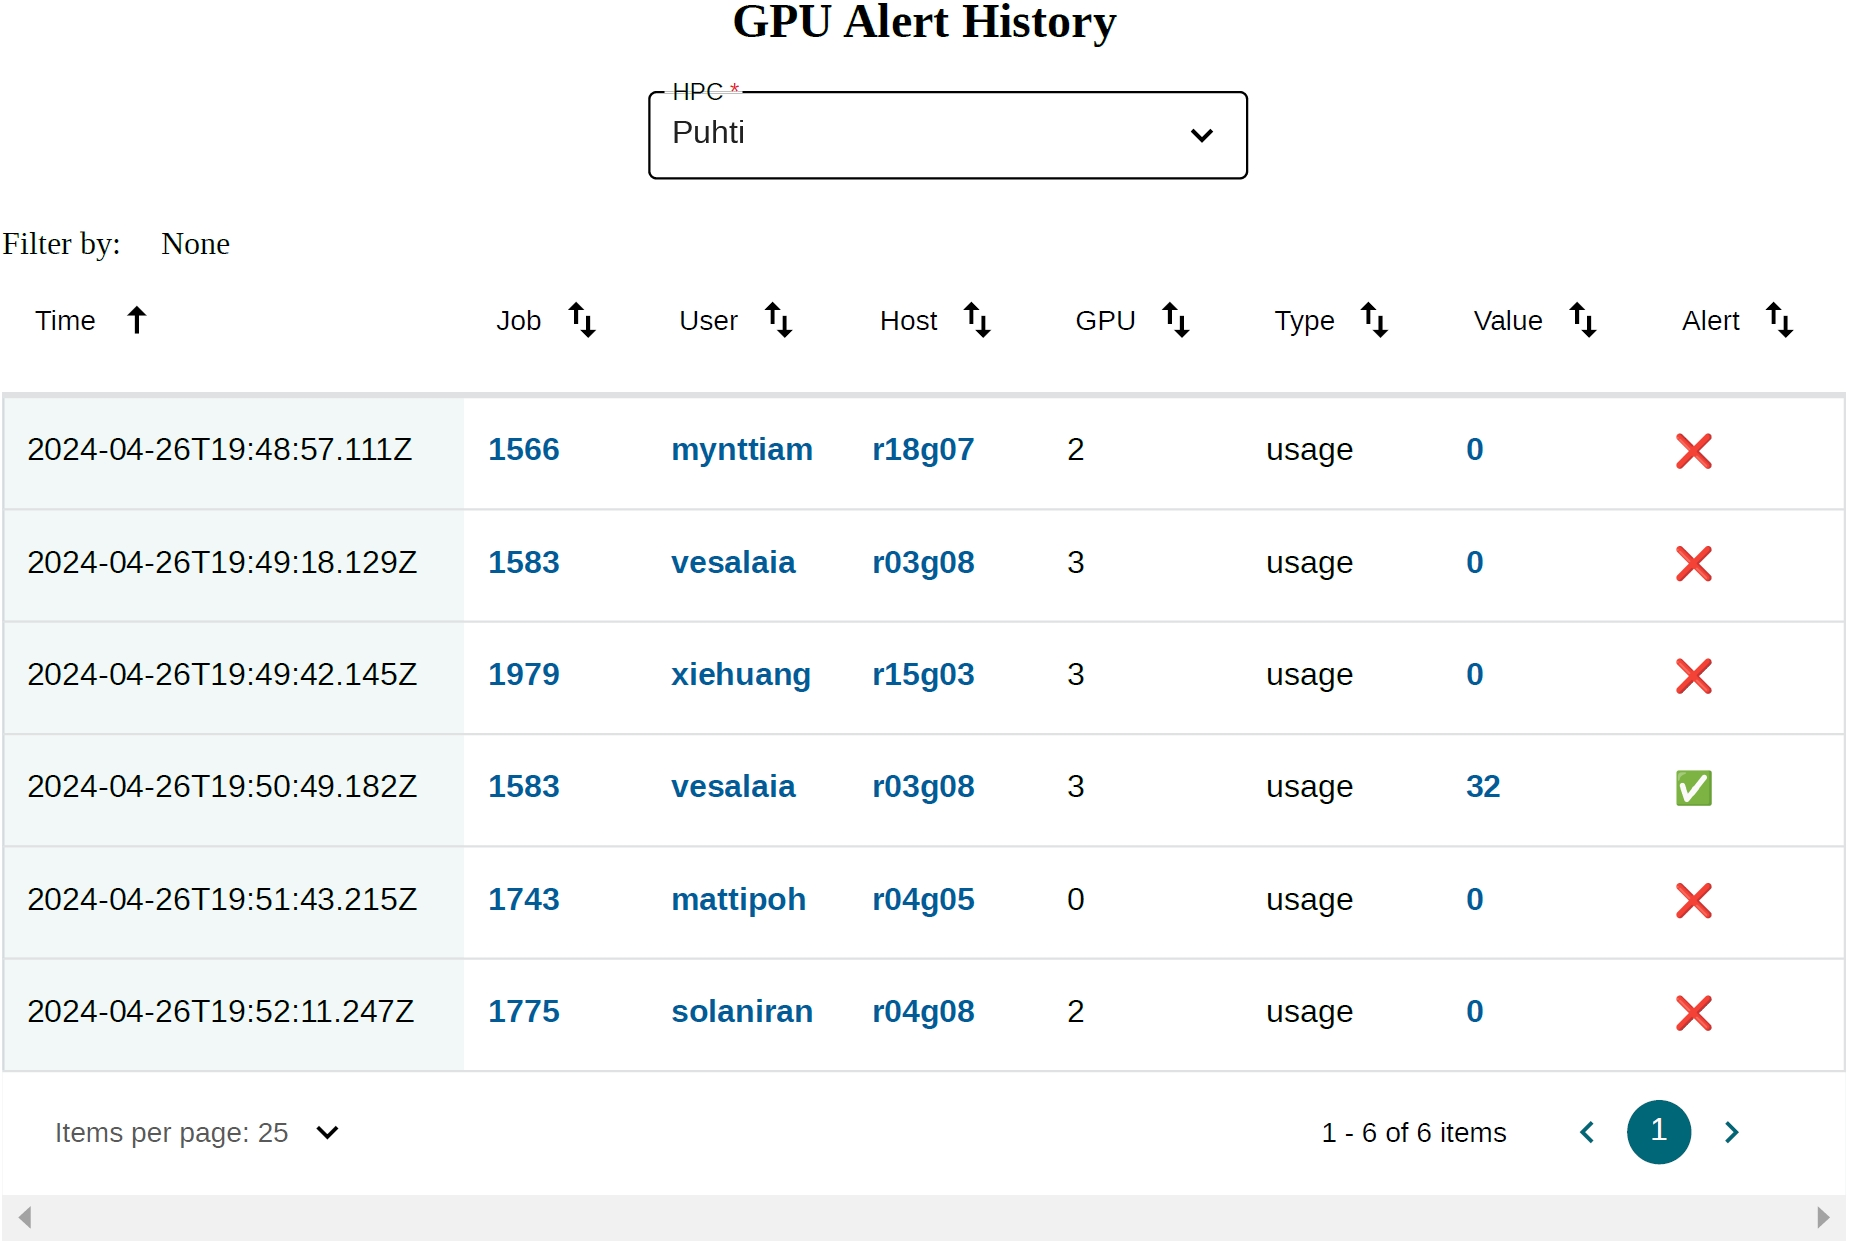
\includegraphics[width=1\textwidth]{figures/history-dashboard.png}
    \caption{GPU alert history dashboard}
    \label{fig_history_dashboard}
\end{figure}

\clearpage
%!TEX root = ../Thesis.tex
\chapter{Results and analysis}
\label{chap:result}
This chapter presents the results from benchmarking the real-time GPU resource monitoring and alerting system in experimental and production setups. The evaluation includes a comprehensive analysis of the system's performance, scalability, and impact on energy efficiency and resource utilization for production within High-Performance Computing (HPC) clusters.

\section{Benchmark}
\subsection{Experimental setup}
\label{subsection:experiment}
The experimental setup involves deploying the proposed GPU monitoring system in a controlled environment, that emulates the characteristics of a typical HPC cluster. The monitoring infrastructure continuously collects and analyzes the simulated GPU metrics, and an alert service is configured to notify any sub-optimal GPU resource utilization.

To integrate all the components for testing, we deployed Slurm in a containerized environment with an isolated network to simulate the actual HPC job context. Everything, including the software versions, replicates what we have in production. We use Podman as the container runtime and Rocky Linux 8 as the base container image to keep up with the operating system we use in Puhti and Mahti (RHEL 8).

We have two compute nodes in our test environment. All the containers are listed as follows:
 
\begin{itemize}
    \item \textbf{mysql}: Database for Slurm to store job data.
    \item \textbf{slurmctld}: Central controller daemon of Slurm monitors all other Slurm daemons and resources, accepts jobs, and allocates resources.
    \item \textbf{slurmdbd}: Interface to the MySQL database for Slurm can be used to archive accounting records.
    \item \textbf{cpn01}: Compute node 1 for executing actual jobs received by Slurm.
    \item \textbf{cpn02}: Compute node 2 for executing actual jobs received by Slurm.
    \item \textbf{frontend}: Similar to the login node in HPC for submitting jobs.
    \item \textbf{timescaledb}: TimescaleDB instance for storing the monitoring data.
    \item \textbf{timescaleingest}: Timescale Ingest instance for ingesting the monitoring data into TimescaleDB.
    \item \textbf{timescalereader}: Timescale Reader instance for fetching the monitoring data and serving as the API for displaying to end users.
    \item \textbf{timescalealert}: Timescale Alert instance for checking the alerts and displaying related information.
    \item \textbf{ondemand}: Open OnDemand serves as a web-based UI to computer clusters in HPC, in addition to SSH access, to help new users who are not familiar with Linux get started quickly. It offers an intuitive entry point for straightforward tasks and shell access for more intricate operations.
    \item \textbf{ldap}: Lightweight Directory Access Protocol (LDAP), required for access control in Open OnDemand.
\end{itemize}

To make testing easier with an arbitrary number of GPUs in a container without needing them, we created a fake Nvidia library that implements the Nvidia-ML interface for generating random metrics data.

We also have separate testing setups for each component, either by randomly generated data or by replaying the data we collected in production from the database dump.

\begin{itemize}
    \item For the random data benchmark, we spawn maximum 23824 (2978*8) Go routines that write to the database simultaneously, which is, i.e. the maximum GPU number we have in LUMI, to simulate the heaviest situation we can have in the pre-exascale supercomputer.
    \item For real data replaying, we read all the records from the database dump ordered by time stamp, and send it to timescale ingest with accelerated speed to reproduce the production situation.
\end{itemize}

\subsection{Performance}
\label{subsec:performance}
The benchmarking process focused on evaluating the system's responsiveness in detecting anomalies and the overall impact on system performance during monitoring, to assess the system's adaptability and robustness in different usage patterns.

We use the local environment to run the container setup mentioned in Subsection \ref{subsection:experiment} on the 12th Gen Intel Core i7-12700H CPU with SSD and 16 GB of RAM by writing random GPU metrics data to the database continuously in an infinite loop, without any interval for writing and dumping data. We run each solution for 10 minutes and take the average of the last 2-minute delay. The benchmark result is shown in Figure \ref{fig_benchmark}:

% import matplotlib.pyplot as plt

% # Data
% methods = ["Polling CAGG", "Polling Direct Query", "Trigger CAGG", "Trigger in Memory"]
% colors = ["#36A2EB", "#FF6384", "#FF9F40", "#9966FF"]
% gpu_write_delay = [
%     [0.321007643, 0.660196607, 1.279614867, 2.433749516, 5.131623884, 11.624568741],
%     [0.31859915, 0.625456453, 1.191235464, 2.350517039, 4.958478354, 9.977873813],
%     [0.765987412, 1.609155407, 2.73052539, 5.176909349, 10.908855175, 20.96940738],
%     [0.65528452, 1.285481557, 2.53125466, 5.007170087, 9.824896244, 19.604722893]
% ]
% read_iteration = [
%     [1.201504459, 2.102009134, 3.58900885, 7.282948943, 13.567867101, 18.581255946],
%     [2.245655323, 3.443534234, 6.191009134, 12.676023435, 26.139007435, 55.204802484],
%     [13.184558, 30.957367, 56.111442, 101.592729, 212.071778, 433.089509],
%     [12.250112, 30.117734, 52.671703, 91.90153, 188.53631, 388.158221]
% ]
% index = range(len(gpu_write_delay[0]))

% # Plot for GPU Write Delay
% fig, axes = plt.subplots(3, 1, figsize=(8, 12))

% for i, method in enumerate(methods):
%     axes[0].bar([x + i * 0.2 for x in index], gpu_write_delay[i], 0.2, label=method, color=colors[i])

% axes[0].set_xlabel('Node Count * GPU')
% axes[0].set_ylabel('Time (s)')
% axes[0].set_title('Delay in Database Writing Transaction Commit')
% axes[0].set_xticks([x + 0.2 * 3 / 2 for x in index])
% axes[0].set_xticklabels(['93*8', '186*8', '372*8', '744*8', '1489*8', '2978*8'])
% axes[0].legend()

% # Plot for Read Iteration
% for i in range(2):
%     method = methods[i]
%     axes[1].bar([x + i * 0.2 for x in index], read_iteration[i], 0.2, label=method, color=colors[i])

% axes[1].set_xlabel('Node Count * GPU')
% axes[1].set_ylabel('Time (s)')
% axes[1].set_title('Time Needed in Completing a Read Loop Iteration')
% axes[1].set_xticks([x + 0.2 * 3 / 2 for x in index])
% axes[1].set_xticklabels(['93*8', '186*8', '372*8', '744*8', '1489*8', '2978*8'])
% axes[1].legend()

% # Plot for Read Iteration
% for i in range(2, 4):
%     method = methods[i]
%     axes[2].bar([x + i * 0.2 for x in index], read_iteration[i], 0.2, label=method, color=colors[i])

% axes[2].set_xlabel('Node Count * GPU')
% axes[2].set_ylabel('Time (ms)')
% axes[2].set_title('Delay in Completing a Memory Status Dump')
% axes[2].set_xticks([x + 0.2 * 3 / 2 for x in index])
% axes[2].set_xticklabels(['93*8', '186*8', '372*8', '744*8', '1489*8', '2978*8'])
% axes[2].legend()

% plt.tight_layout()
% plt.savefig("benchmark-data.pdf")

\begin{figure}[H]
    \centering
    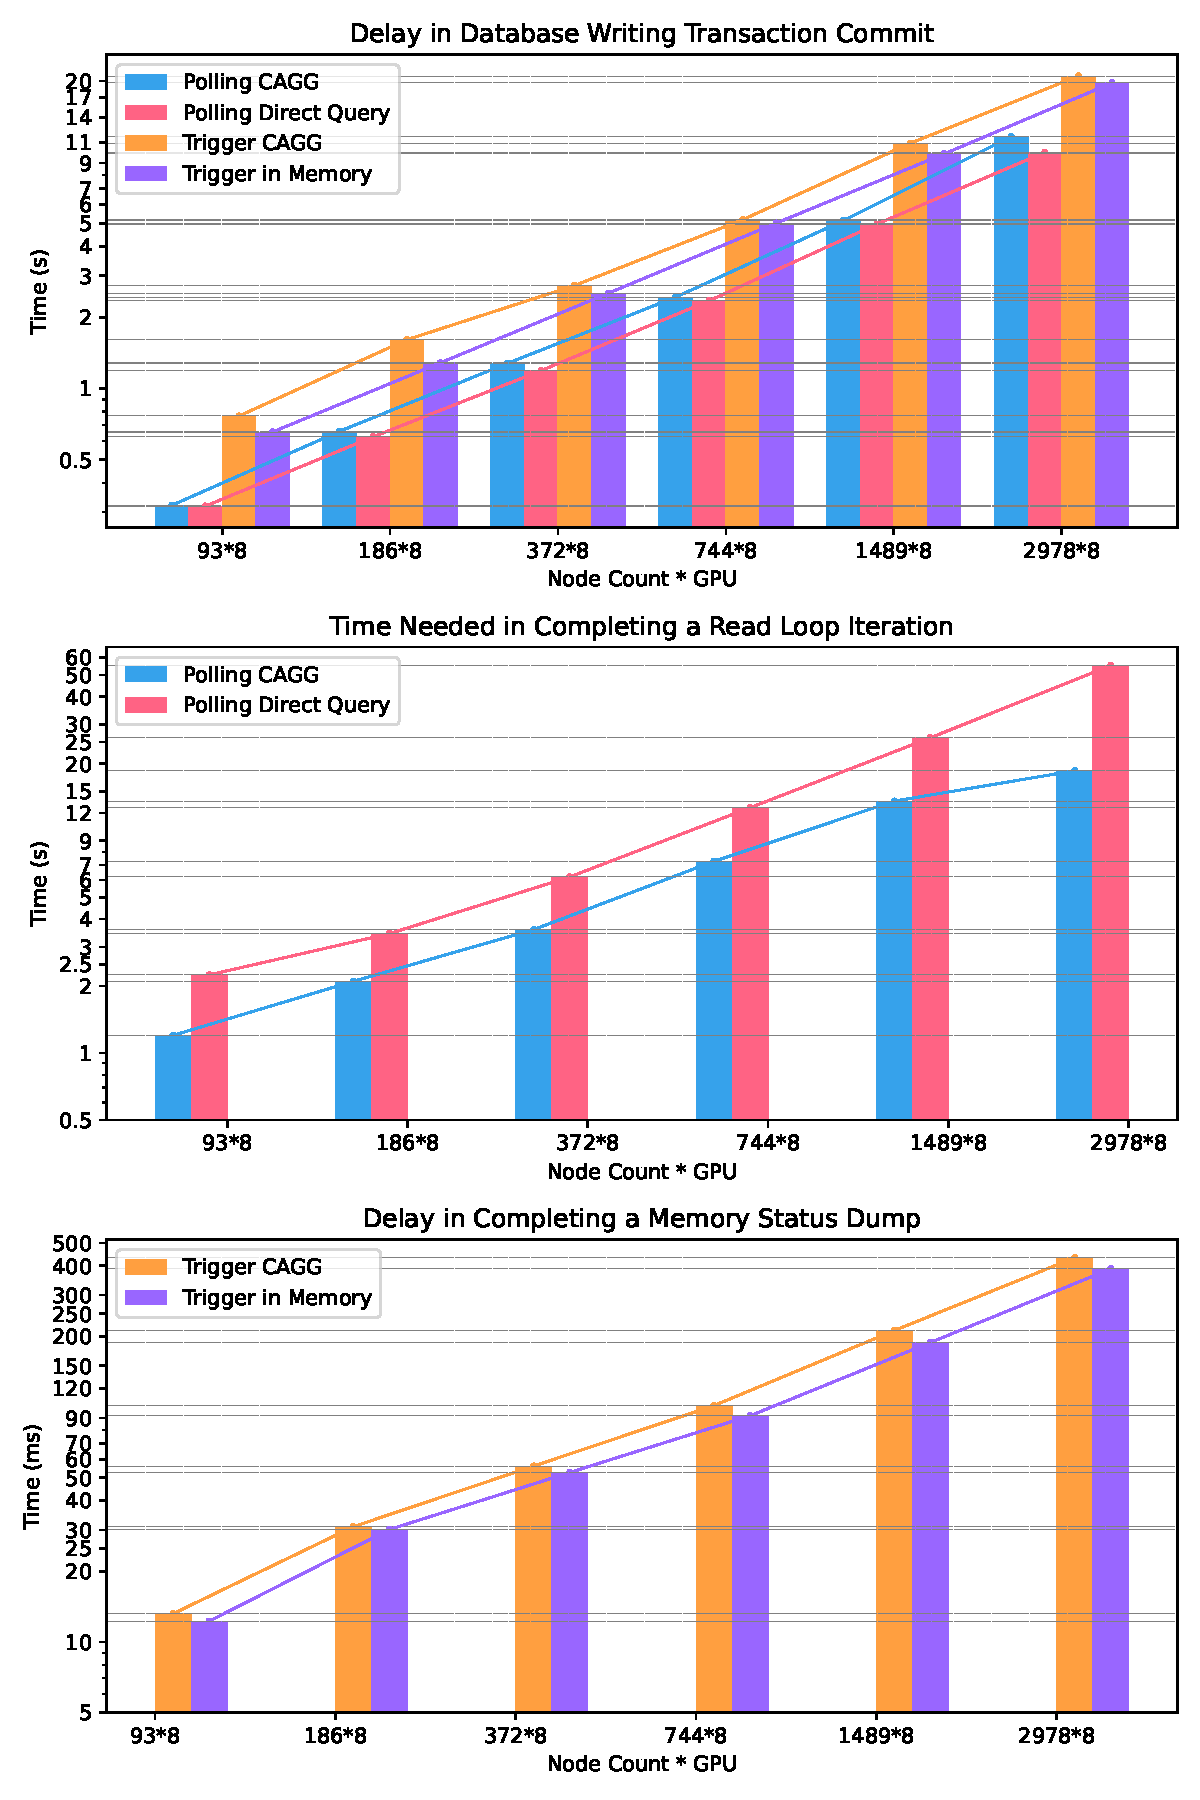
\includegraphics[width=1\textwidth]{figures/benchmark-data.pdf}
    \caption{Timescale Alert benchmark result}
    \label{fig_benchmark}
\end{figure}

From Figure \ref{fig_benchmark}, we can learn that:

\begin{itemize}
    \item Generally, all the delays scale linearly with the number of GPUs.
    \item Triggers generally double the delay in database transaction commit time for writing, which the overhead of NOTIFY should be the cause.
    \item Continuous aggregates (CAgg) cause a slight increase in writing delay and the memory status dump delay for the triggers solution, which is likely to be caused by the overhead of CAgg background jobs. However, CAgg accelerates the query speed dramatically compared to traditional SQL queries aggregate, as we can see a significant time reduction in completing a read loop among all the jobs available.
    \item Polling is very inefficient for accessing data in real-time, since it creates a delay that is almost 100x more than the triggers solution.
\end{itemize}

Hence, the results confirmed our empirical analysis in Section \ref{sec:alertservice} and led to the final design we used after comparison: \textbf{triggers without continuous aggregates}. The reason is that triggers have the best real-time access, while only doubling the delay in writing compared to polling, which is acceptable, and the in-memory solution has a better performance in both read and write delay. Most importantly, the in-memory solution allows us to access raw data for more complicated statistics calculations and use machine learning models. We used the Golang data race detector to ensure the correctness during benchmarking and testing. We also checked the memory usage during the benchmark: The maximum Resident Set Size (RSS) is around 84.6 MB, which is also acceptable.

%CPU %MEM    VSZ   RSS 21.0  0.5 3184092 84612

\section{Production}

The production evaluation involved deploying the real-time GPU monitoring system in a live HPC environment, specifically on the Puhti and Mahti systems at the CSC -- IT Center for Science, which allows us to test the practicability in alerting for real-world workloads from diverse scientific domains, including molecular dynamics simulations, computational chemistry, and machine learning. Unfortunately, due to the time limit for the thesis writing process, we are not able to finish the deployment of the whole monitoring and alert services in production for the pre-exascale HPC system, LUMI, but we have already verified this possibility in Section \ref{subsection:experiment} through a benchmark.

% We intended to deploy this whole infrastructure on LUMI as well. Unfortunately, we were unable to do so during the thesis writing period due to the shortage of administrators on the LUMI side.

The production evaluation focused on the practical implications of integrating the alerting and monitoring system into the daily operations of HPC clusters. Key performance indicators, such as the system's ability to facilitate timely alerts, were measured. Additionally, the impact on user experience was evaluated considering the introduction of real-time alerts to administrators.

\subsection{Setup}

As is presented in Figure \ref{fig_monitoring_production_development}, we have two copies of the monitoring infrastructure separately for Puhti and Mahti deployed as microservices inside containers:

\begin{figure}[H]
    \centering
    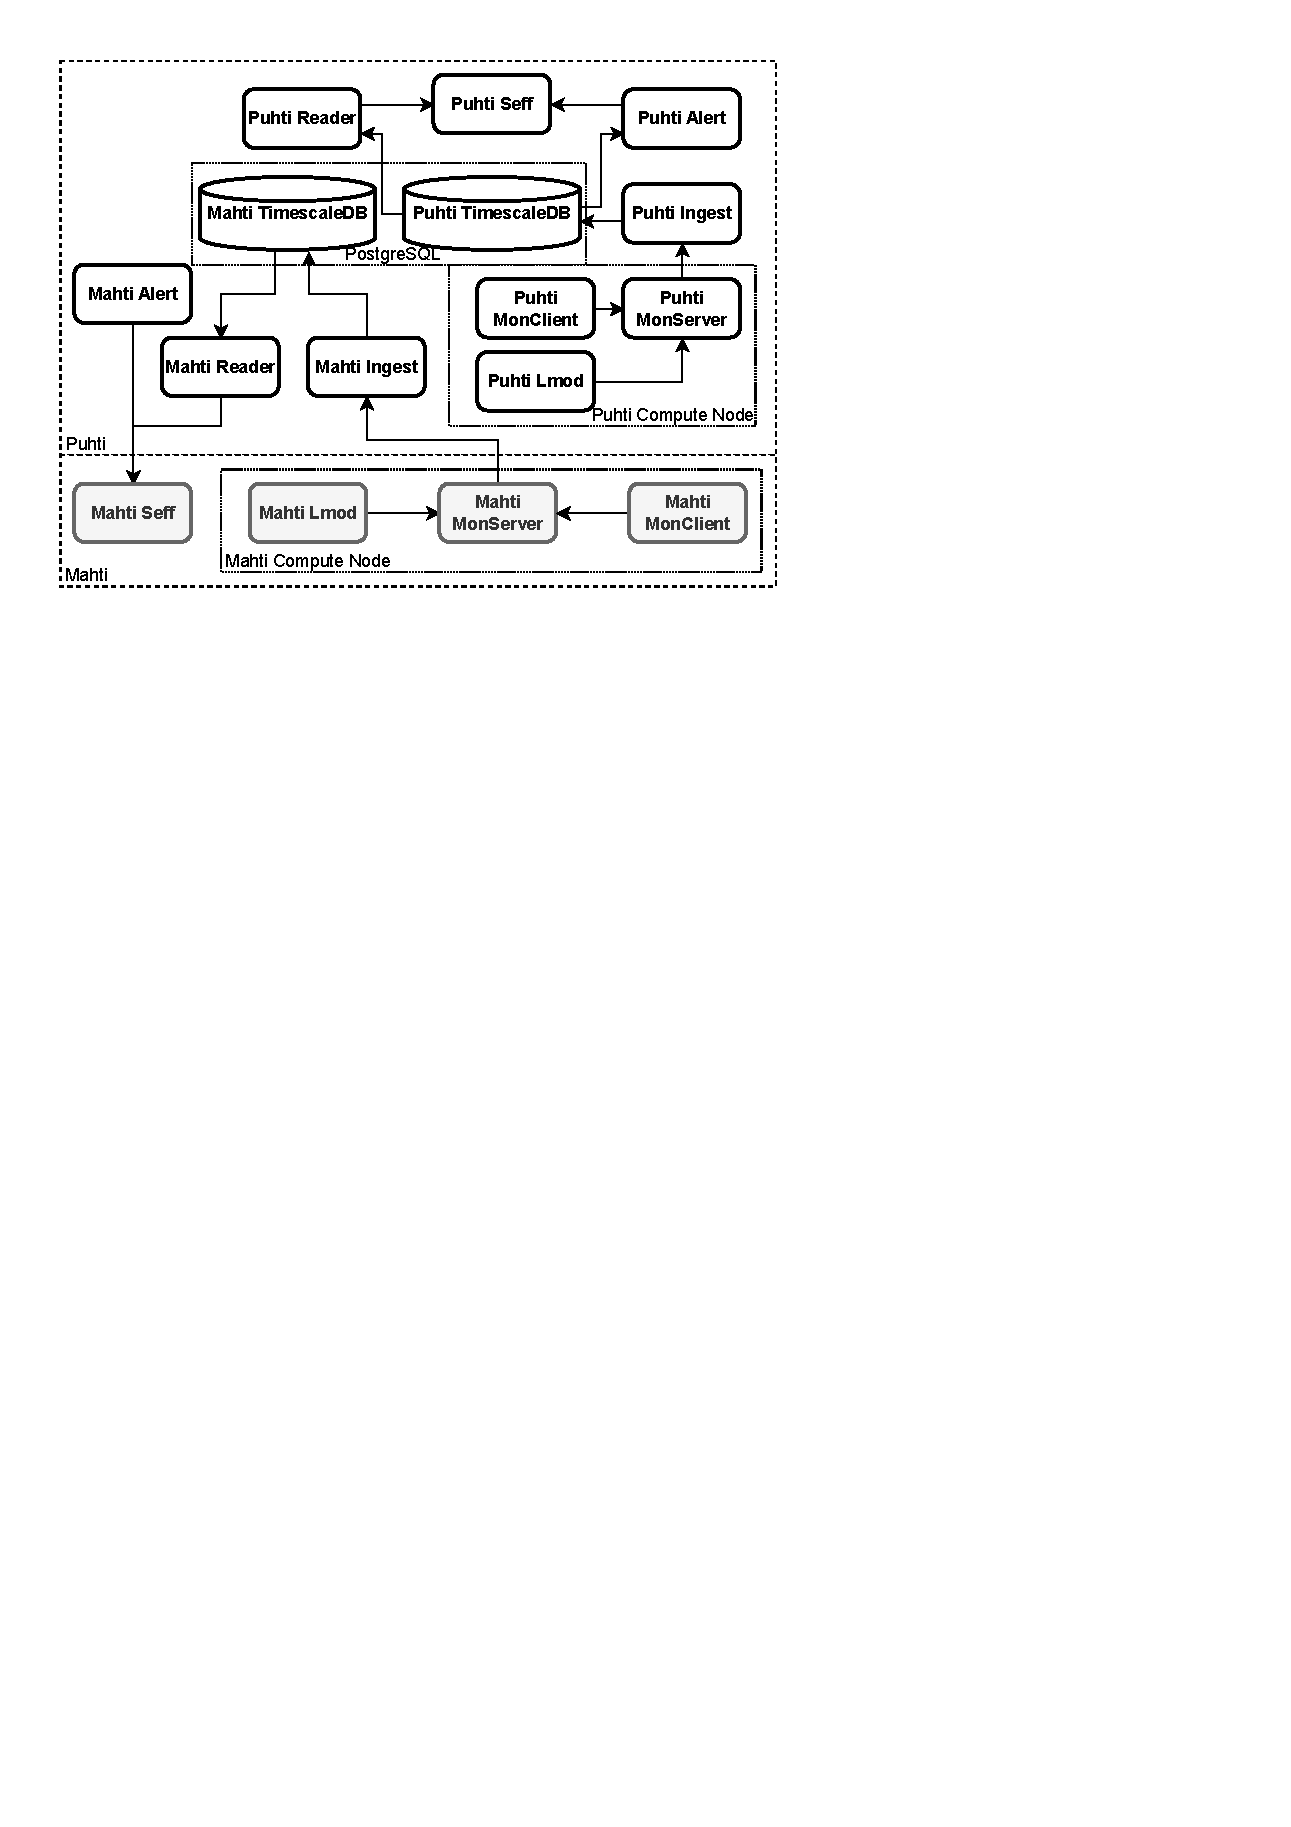
\includegraphics[width=1\textwidth]{figures/production-deployment.pdf}
    \caption{GPU monitoring infrastructure production setup for Puhti and Mahti}
    \label{fig_monitoring_production_development}
\end{figure}

\begin{itemize}
    \item \textbf{Monitoring Daemon} is written in C++ and deployed on each compute node for both Puhti and Mahti. The \textbf{Monitoring Server} is deployed as a systemd service. In contrast, the \textbf{Monitoring Client} is deployed as a CLI utility to be called by the Slurm prolog and epilog scripts.
    \item \textbf{Lmod} is the environment module system in Lua. It is deployed on each compute node as well.
    \item \textbf{Timescale Reader}, \textbf{Timescale Ingest}, and \textbf{Timescale Alert} are all written in Go and deployed as systemd services. Both copies for Mahti and Puhti are deployed on the Puhti MonDB Utility node.
    \item \textbf{TimescaleDB} is deployed as a plugin on the PostgreSQL node. We use different database names to isolate the monitoring data between Puhti and Mahti.
    \item \textbf{Seff} script is the CLI utility written in Perl. It is installed as an RPM package by admins in all the nodes and can be called by the user.
    \item Other \textbf{visualization} services, such as the job history and alert status dashboard, are deployed as Flask Apps for Open OnDemand.
\end{itemize}

We set the alert sliding window size at 30 minutes. Initially, we collected the monitoring data at 1-minute intervals, then increased that to 20 seconds, and the whole monitoring and alert system was still stable enough. We set the compression policy to compress the data after one day and do the retention every half-year. We also put an index on the hostname, job ID, and GPU ID to accelerate the querying speed on the database.

\subsection{Case studies}
Here are some real-world scenarios, where we use our monitoring infrastructure and Timescale Alert to help users solve issues when they submit jobs in HPC. These case studies illustrate how the system proposed in this thesis enables the support team to proactively identify, diagnose, and resolve issues, ensuring efficient utilization of HPC resources, reducing user queuing time, and improving user satisfaction.

\subsubsection{Configuration Error}
From the GPU alert status dashboard, the user support team was alerted by a job that reserved 2 full nodes, each with 4 A100 GPUs. It has nearly 100\% usage almost all the time for 1 GPU but zero usage for the remaining 7, as illustrated in Figure \ref{fig_job_config_error}. By checking the GPU alert history dashboard, the support team found that the alert began a long time ago, the disk I/O currently used by that job is low, so it shouldn't be the case that the job is still loading data. The situation leads them to suspect a configuration error or code bug. By examining the module load information stored in the job metadata, they discovered that Pytorch was loaded into the job context, which is a mature machine-learning library and shouldn't have such a situation if everything is configured right. The user support team then contacted the user to investigate possible configuration errors. It was eventually discovered that \texttt{CUDA\_VISIBLE\_DEVICES} was mistakenly set to \texttt{0} (utilizing only 1 GPU), and they didn't use \texttt{srun} to properly distribute the job step to all nodes they applied for with \texttt{torchrun}. To fix this, the job was terminated, and a new job with the correct configuration was subsequently submitted.

\begin{figure}[H]
    \centering
    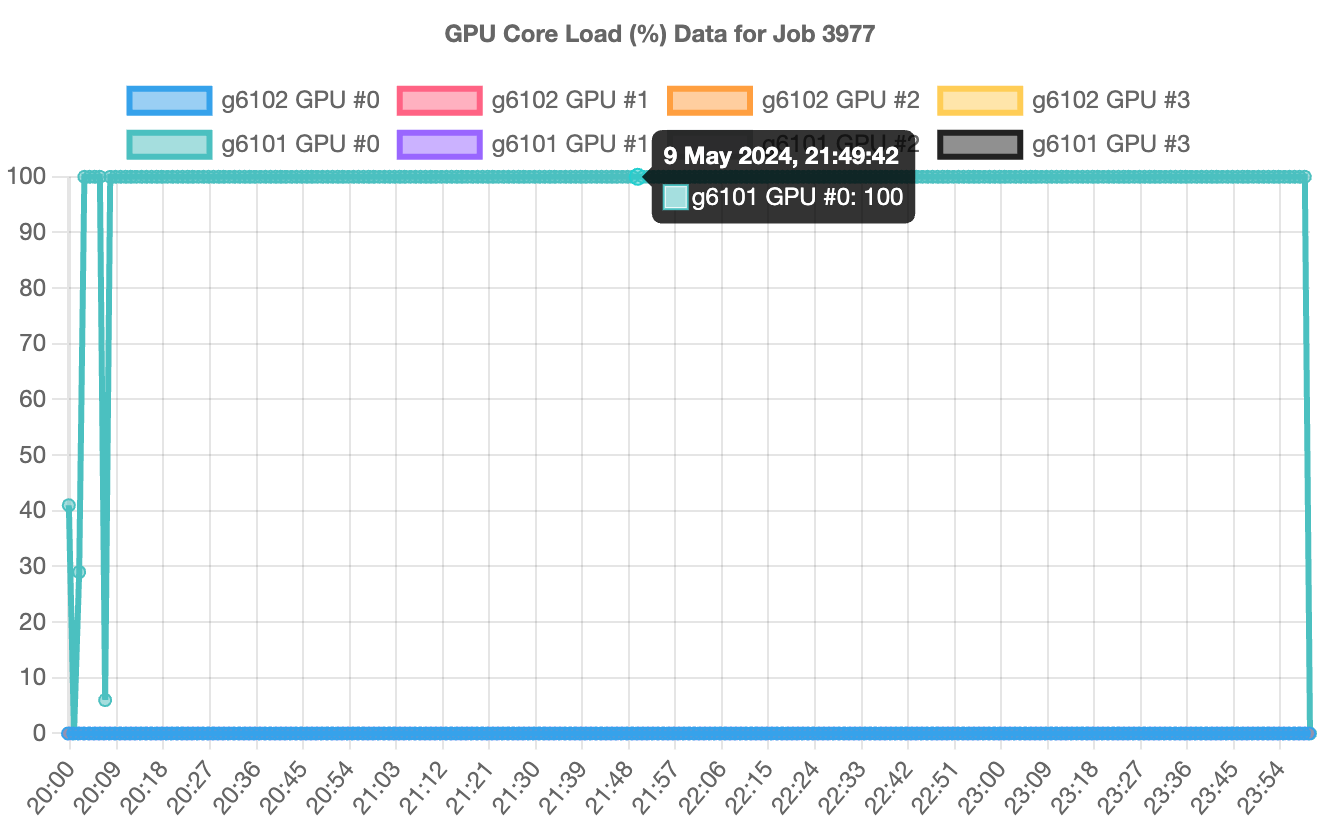
\includegraphics[width=1\textwidth]{figures/job-config-error.png}
    \caption{Job usage graph for the one with configuration error}
    \label{fig_job_config_error}
\end{figure}

\subsubsection{Code Bugs}
In another scenario, the support team received a similar situation of alerts described in the \textit{Configuration Error} about a job that was allocated multiple GPUs, but showed low utilization on all GPUs except a few of them, but those with high usage always change and take turns, as demonstrated in Figure \ref{fig_job_code_bugs}. By analyzing the job's execution patterns, as well as checking with the user, they found that the workload was not properly distributed across the GPUs because of code bugs and how the user's code was written. The user was advised on how to improve their code to better parallelize their tasks and fully utilize the allocated GPUs. This resulted in significantly improved performance and more efficient use of the cluster's GPU resources.

\begin{figure}[H]
    \centering
    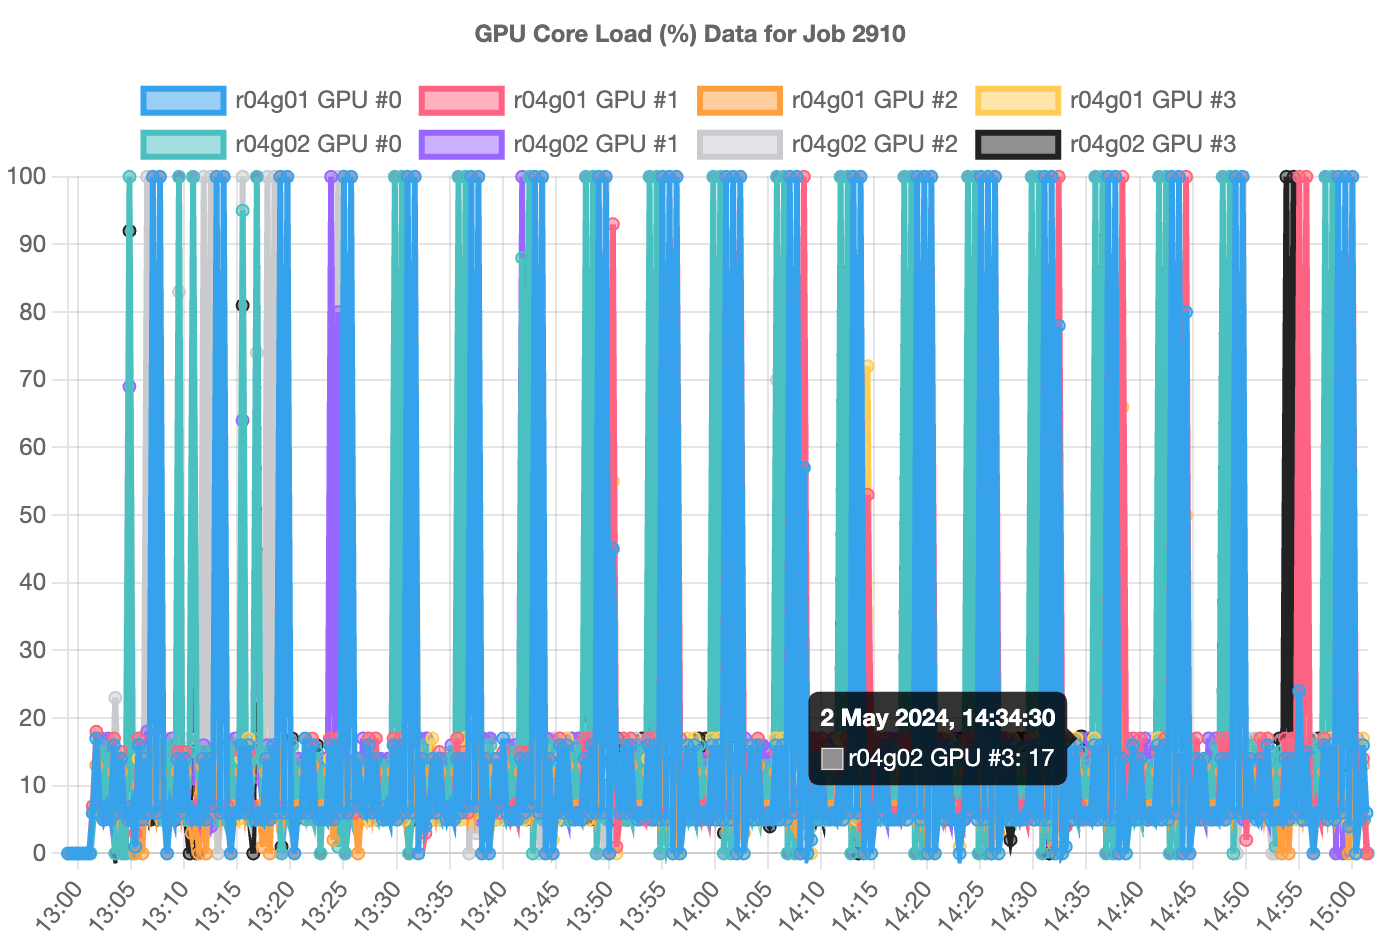
\includegraphics[width=1\textwidth]{figures/job-code-bugs.png}
    \caption{Job usage graph for the one with code bugs}
    \label{fig_job_code_bugs}
\end{figure}

\subsubsection{GPU Over-Provisioning}
For most cases, the support team was alerted by jobs with low overall GPU utilization across all allocated GPUs, as shown in Figure \ref{fig_gpu-usage-graph} and Figure \ref{fig_job_over_provison} for examples. After contacting the users, most of the time it was found that their applications did not scale well beyond a certain number of GPUs, which means they were allocated more GPUs than needed, resulting in under-utilization of the resources. In the end, the support team recommended shrinking the GPU requests to better match the application's needs, leading to more efficient resource usage and freeing up GPUs for other jobs.

\begin{figure}[H]
    \centering
    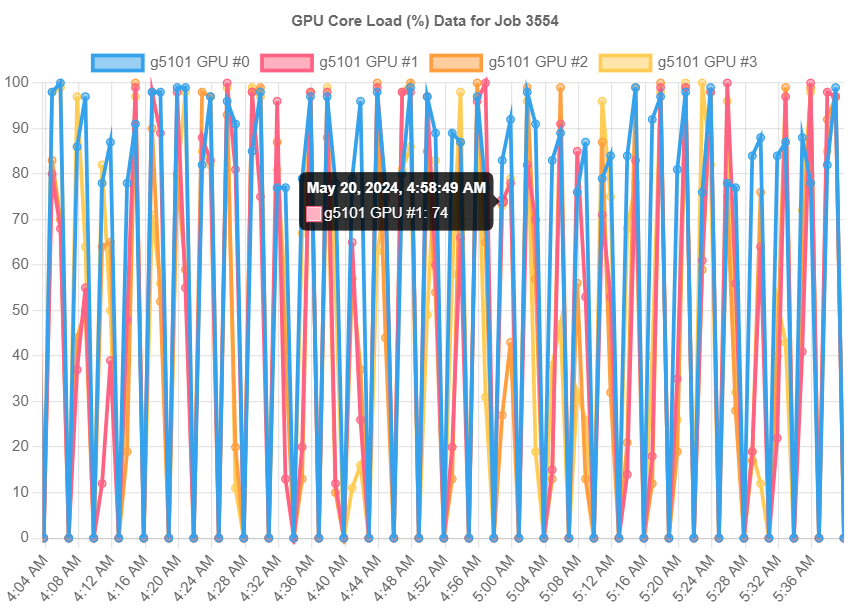
\includegraphics[width=1\textwidth]{figures/job-over-provison.png}
    \caption{Job usage graph for the one with over provision}
    \label{fig_job_over_provison}
\end{figure}

\subsubsection{Interactive use on GPU compute node}
For some cases, the support team also gets alerted by jobs that only requested 1 GPU but still with low GPU utilization, on partitions that were meant for heavy GPU computing jobs, as demonstrated in Figure \ref{fig_job_interactive} for one example. After checking with the users, most of the time it was found that they are developing their code interactively. The user then was suggested to switch their job to the partition that is meant for lightweight GPU computing.

\begin{figure}[H]
    \centering
    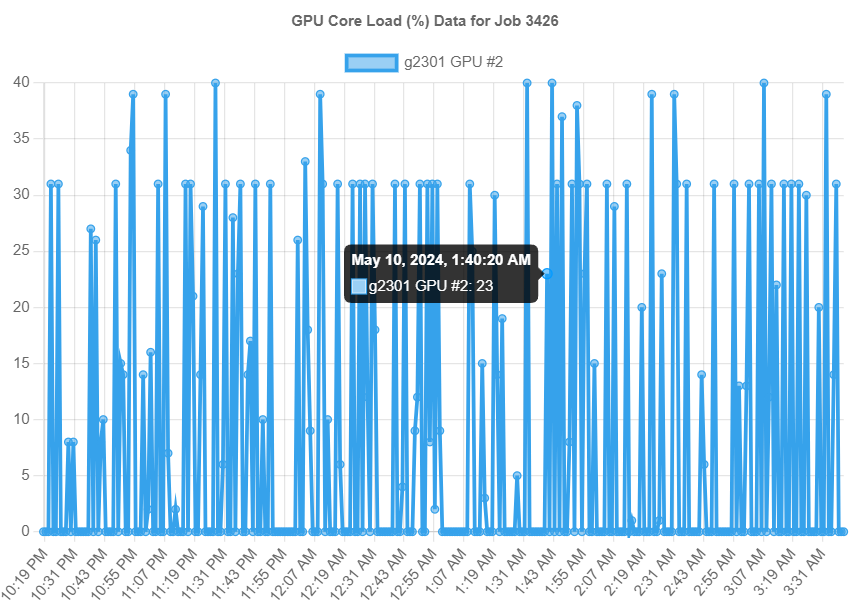
\includegraphics[width=1\textwidth]{figures/job-interactive.png}
    \caption{Job usage graph for the one with interactive usage on heavy GPU compute partition}
    \label{fig_job_interactive}
\end{figure}

\subsubsection{GPU Memory Leaks}
A user raised a ticket, asking for help from the user support team about why his long-running AI inference job eventually crashed after some time. After checking the monitoring history, as shown in Figure \ref{fig_job_memory_leak}, the support team found progressively increasing GPU memory usage, which ultimately led to the job being killed due to exceeding memory limits. The support team worked with the user to review the code and identified a memory leak caused by improper handling of GPU memory allocations in a loop. The memory usage was stabilized by fixing the code, allowing the job to be finished successfully without exceeding memory limits.

\begin{figure}[H]
    \centering
    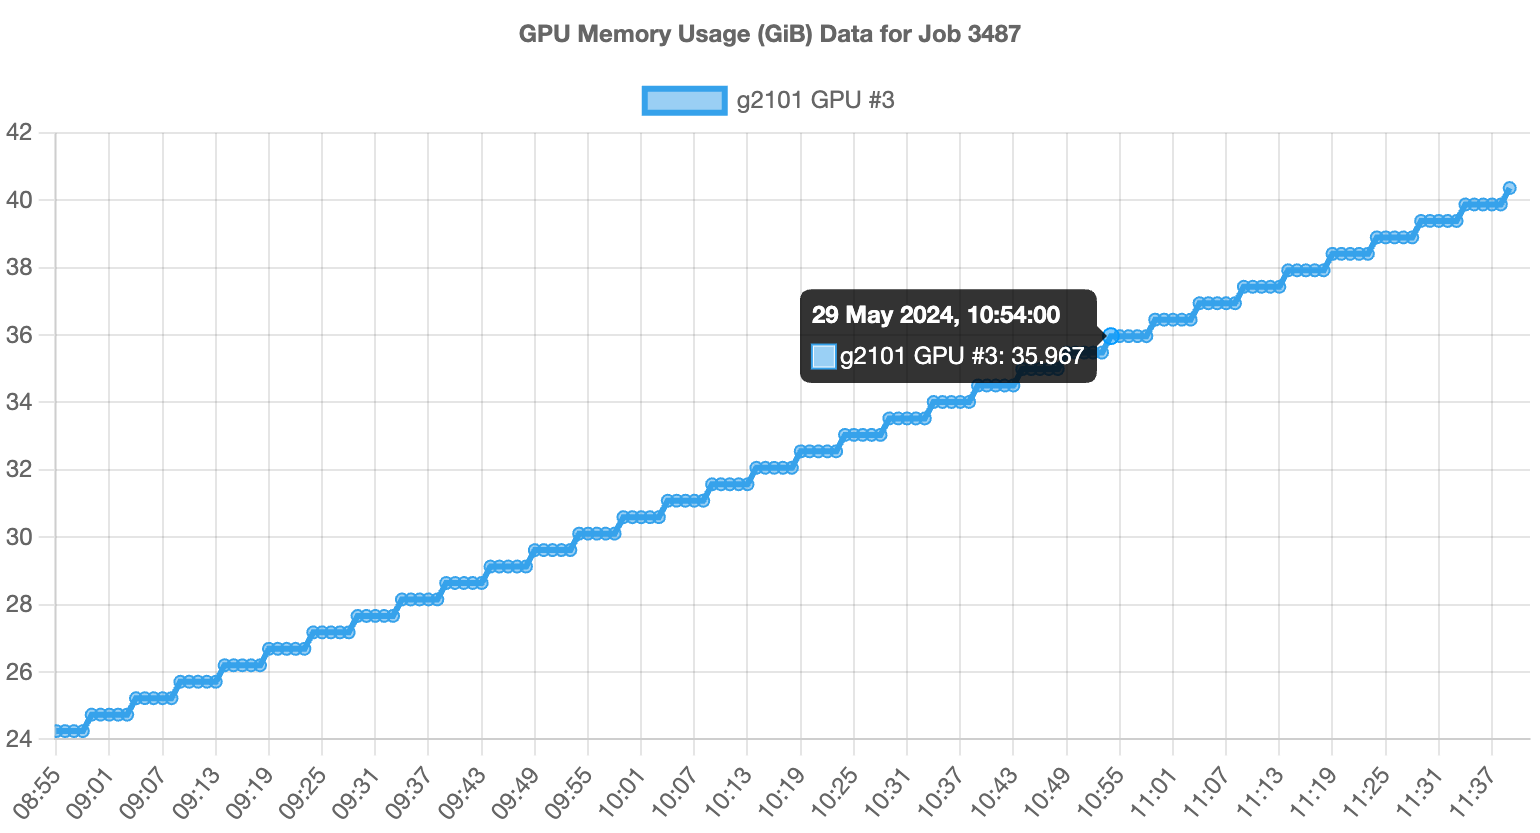
\includegraphics[width=1\textwidth]{figures/job-memory-leak.png}
    \caption{Job usage graph for the one with GPU memory leaks}
    \label{fig_job_memory_leak}
\end{figure}

\clearpage
%!TEX root = ../Thesis.tex
\chapter{Discussion}
\section{Findings}
Several key insights have been garnered through developing and implementing the monitoring system and alert service for GPU resource utilization in HPC clusters, paving the way for further exploration and advancement in this domain.

One of the primary findings of this research is the effectiveness of the implemented algorithms in detecting inefficient GPU resource usage. By analyzing real-time monitoring data, the system can identify instances where jobs are not effectively utilizing allocated GPU resources, potentially leading to performance bottlenecks or resource wastage. This capability is crucial for optimizing job scheduling and resource allocation in HPC environments, ultimately enhancing overall system efficiency and throughput.

Moreover, integrating GPU energy consumption data into the monitoring system offers valuable insights into the sustainability aspects of HPC operations. With increasing focus on energy efficiency and environmental sustainability, understanding and managing power consumption in HPC clusters is paramount. By monitoring GPU energy usage and identifying energy-intensive tasks or jobs, HPC users can implement strategies to reduce power consumption, lower operational costs, and minimize their environmental footprint.

Furthermore, the research's practical implications extend beyond HPC cluster management to various application domains, including AI development and scientific computing. The ability to monitor and analyze GPU resource utilization in real time provides researchers and practitioners with valuable insights into the performance of AI algorithms, computational simulations, and data analysis workflows. By optimizing GPU resource allocation and usage, HPC users can accelerate AI model training, improve scientific simulations, and drive innovation in various fields.

Additionally, we highlight the potential challenges and limitations we have tackled in the monitoring system and alert service, such as scalability issues with large-scale HPC clusters and compatibility with different hardware configurations (Nvidia/AMD).

\section{Related work}

Several job monitoring platforms for HPC have emerged in recent years, including Ganglia \cite{MASSIE2004817}, TACC Stats \cite{7081222}, XDMoD \cite{7106398}, LIKWID \cite{8049016}, LDMS \cite{10.1145/3225058.3225086}, PIKA \cite{9229636}, and MAP \cite{9229613,9556031}. However, these platforms lack GPU monitoring support, and few have real-time alerting and history visualization features.

Other notable works in this area use the Prometheus monitoring framework and the Grafana visualization toolkit, including Jobstats \cite{10.1145/3569951.3604396} and the work down by Jaelyn et al. \cite{10.1145/3569951.3597554}. These platforms are designed for both CPU and GPU clusters. It leverages the Prometheus monitoring framework \cite{208870} and the Grafana visualization toolkit \cite{Chakraborty2021} to provide job-level information on CPU/GPU efficiencies and CPU/GPU memory usage. However, these out-of-the-box solutions operate with high-level APIs, and it is hard to access the streaming raw data for alert customization, such as machine learning algorithms to identify jobs in real-time. Performance can also be an issue, and it is tough to debug if something goes wrong when we implement these solutions to pre-exascale supercomputers such as LUMI.

\clearpage
%!TEX root = ../Thesis.tex
\chapter{Conclusions and future work}
\label{chap:conclusions}
In this chapter, we critically analyze and interpret the findings presented in this thesis, focusing on their significance, implications, and potential applications. Then, we conclude with future work that we could not cover during the thesis period.

\section{Summary}

The thesis comprehensively explores designing, implementing, and evaluating a monitoring system and alert service for GPU resource utilization in High-Performance Computing (HPC) clusters. Through a systematic methodology, the research addresses critical challenges in efficiently analyzing jobs in HPC systems in real-time, focusing on minimizing alert delays and performance impacts on database systems, maintaining reliable data structures for job alert status checks, and identifying optimal algorithms for generating alerts, to address all research questions in Section \ref{sec:rqs}.

The thesis's contributions are multifaceted. First, a monitoring system and alert service are successfully created and deployed for Nvidia and AMD GPUs within Slurm-managed supercomputer systems. Then, an algorithm is developed to detect and alert jobs with inefficient GPU resource usage by investigating collected monitoring data. Additionally, the thesis provides insights into GPU resource utilization dynamics. It offers practical applications in advancing generative AI models while promoting sustainability in HPC cluster usage.

The thesis comprises sections dedicated to discussing techniques for building the monitoring system and alert service, detailing the implementation of the proposed system, presenting results from experimental benchmark and production setups, and offering concluding remarks. The methodology includes requirement analysis, system design and architecture, implementation and deployment, data collection and analysis, evaluation and validation, feedback and iterative improvement, documentation, and knowledge transfer.

The thesis illustrates the operationalization of the monitoring system and alert service through JSON strings and SQL code excerpts, showcasing the real-time mechanisms for capturing and processing job metadata and GPU usage data. Triggers and notification functions within the PostgreSQL database enable instantaneous communication and notification of relevant events, facilitating timely updates and actions based on incoming data.

Overall, the thesis contributes to advancing monitoring and alerting systems for GPU resource utilization in HPC clusters, with practical implications for optimizing job scheduling, resource allocation, and overall system efficiency. By addressing critical challenges and proposing innovative solutions, the research enhances the effectiveness and sustainability of GPU-accelerated computing environments, paving the way for future advancements in AI research and HPC infrastructure management.

\section{Future work}
There are several avenues for future research and improvements due to the limited time during this master's thesis project:

\begin{enumerate}
    \item \textbf{Integration with Additional Job Schedulers}: Extend support for real-time GPU monitoring to additional job schedulers commonly used in HPC environments, such as LSF \cite{10.1145/3569951.3597564}, TORQUE \cite{10.1145/1188455.1188464}, or UGE \cite{10.1145/3332186.3338408}, enhancing the compatibility with diverse cluster architectures.
    \item \textbf{More Monitoring Metrics}: Collect monitoring data from other hardware (e.g., CPU, disk I/O) and collectively contribute to the alert for the whole system. The monitoring infrastructure already has the capabilities for monitoring additional hardware, but they have not been tested in production due to performance considerations. In addition, we can also explore the possibility of capturing and analyzing fine-grained GPU usage metrics, including memory bandwidth, cache utilization, and instruction throughput. This granular level of monitoring can provide deeper insights into application performance and identify optimization opportunities at the code level.
    \item \textbf{Flexible Alerting}: Investigate adaptive alerting strategies that dynamically adjust thresholds we use in the alert algorithms currently based on workload characteristics, ensuring effective alerting across varying HPC workloads. It's also worth exploring the integration of possible other advanced machine learning algorithms to predict GPU resource usage patterns, enabling proactive alerting based on historical data analysis. We can also try to implement mechanisms to directly gather feedback from administrators or support teams regarding the effectiveness of the jobs, and improve our alert strategies automatically, so that we can have continuous refinement based on practical usage experiences.
    % Publish hints to HPC users regarding how to fix and improve their job utilization of hardware resources.
    \item \textbf{Resource Optimization}: Investigate optimization techniques for dynamically allocating GPU resources based on real-time workload demands and system utilization. This could involve developing algorithms for intelligent resource provisioning and load balancing to maximize overall cluster efficiency and performance. We can also investigate the predictive maintenance techniques for GPUs based on real-time monitoring data. Predictive maintenance models can anticipate failures or performance degradation by analyzing hardware health metrics and performance degradation, enabling proactive maintenance actions to minimize downtime and maximize system reliability. It's also worth investigating integrating the real-time GPU monitoring system with energy management systems to optimize power consumption and reduce environmental impact. By correlating GPU usage metrics with power consumption data, HPC administrators can implement energy-efficient computing strategies, such as dynamic voltage and frequency scaling, to minimize power consumption without sacrificing performance.
\end{enumerate}

\clearpage
\thesisbibliography

\bibliographystyle{plain}
\bibliography{Bibliography}

\clearpage

\thesisappendix
%!TEX root = ../Thesis.tex
\chapter{Code for drawing Figure \ref{fig_silhouette_directly} \& Figure \ref{fig_silhouette_statistics}}
In Section \ref{sec:algo_method}, we have the silhouette analysis on windowed GPU load data. Here is the code for the direct one, as in Figure \ref{fig_silhouette_directly}. Note that for \texttt{load\_gpu.csv}, we have the format as follows, where the data for each entry is the fixed-size (30) sliding window:

\begin{equation*}
hostname,job id,GPU id,data 0,data 1,....,data 28,data 29
\end{equation*}

\begin{lstlisting}[language=Python]
import pandas as pd

data = pd.read_csv('load_gpu.csv', usecols=[i for i in range(3, 33)])
X = data.to_numpy()

import matplotlib.cm as cm
import matplotlib.pyplot as plt
import numpy as np

from sklearn.cluster import KMeans
from sklearn.metrics import silhouette_samples, silhouette_score

range_n_clusters = [2, 3, 4, 5, 6, 7]

plt.rcParams.update({'font.size': 56})

for n_clusters in range_n_clusters:
    print("Start creating plot for n_clusters =", n_clusters)
    # Create a subplot with 1 row and 1 column
    fig, ax1 = plt.subplots(1, 1)
    fig.set_size_inches(18, 18)

    # The 1st subplot is the silhouette plot
    # The silhouette coefficient can range from -1, 1
    ax1.set_xlim([-0.6, 0.4])
    # The (n_clusters+1)*10 is for inserting blank space between silhouette
    # plots of individual clusters, to demarcate them clearly.
    ax1.set_ylim([0, len(X) + (n_clusters + 1) * 10])

    # Initialize the clusterer with n_clusters value and a random generator
    # seed of 10 for reproducibility.
    clusterer = KMeans(n_clusters=n_clusters)
    cluster_labels = clusterer.fit_predict(X)
    print(cluster_labels, cluster_labels.shape)

    # The silhouette_score gives the average value for all the samples.
    # This gives a perspective into the density and separation of the formed
    # clusters
    silhouette_avg = silhouette_score(X, cluster_labels)
    print(
        "For n_clusters =",
        n_clusters,
        "The average silhouette_score is :",
        silhouette_avg,
    )

    # Compute the silhouette scores for each sample
    sample_silhouette_values = silhouette_samples(X, cluster_labels)

    y_lower = 10
    for i in range(n_clusters):
        # Aggregate the silhouette scores for samples belonging to
        # cluster i, and sort them
        ith_cluster_silhouette_values = sample_silhouette_values[cluster_labels == i]

        ith_cluster_silhouette_values.sort()

        size_cluster_i = ith_cluster_silhouette_values.shape[0]
        y_upper = y_lower + size_cluster_i

        color = cm.nipy_spectral(float(i) / n_clusters)
        ax1.fill_betweenx(
            np.arange(y_lower, y_upper),
            0,
            ith_cluster_silhouette_values,
            facecolor=color,
            edgecolor=color,
            alpha=0.7,
        )

        # Label the silhouette plots with their cluster numbers at the middle
        ax1.text(-0.05, y_lower + 0.5 * size_cluster_i, str(i))

        # Compute the new y_lower for next plot
        y_lower = y_upper + 10  # 10 for the 0 samples

    # ax1.set_title("The silhouette plot for the various clusters.")
    ax1.set_xlabel("The silhouette coefficient values")
    ax1.set_ylabel("Cluster label")

    # The vertical line for average silhouette score of all the values
    ax1.axvline(x=silhouette_avg, color="red", linestyle="--")

    ax1.set_yticks([])  # Clear the yaxis labels / ticks
    ax1.set_xticks([-0.6, -0.4, -0.2, 0, 0.1, 0.2, 0.3, 0.4])

    plt.savefig("plot/directly/silhouette_directly_" + str(n_clusters) + ".pdf", format="pdf", bbox_inches="tight")

plt.show()
\end{lstlisting}

For the one with statistics analysis, as in Figure \ref{fig_silhouette_statistics}, the code for drawing it is similar, the only difference is that, we do an aggregation for each entry (fixed-size (30) sliding window), and append those result to the end of each entry, using the nine descriptive statistics metrics, as defined in Subsection \ref{subsec:statistics}: percentiles (25\%, 50\%, 75\%), kurtosis, maximum, minimum, skewness, standard deviation, as well as variance.

\clearpage
%!TEX root = ../Thesis.tex
\chapter{Code for drawing Figure \ref{fig_load_gpu_histogram_1} \& Figure \ref{fig_load_gpu_histogram_2}}
In Section \ref{sec:algo_method}, we also have the histogram of statistics analysis on windowed GPU load data. Here is the code for drawing those figures:

\begin{lstlisting}[language=Python]
import pandas as pd
import matplotlib.pyplot as plt
plt.rcParams.update({'font.size': 32})
plt.figure(figsize=(14,4))

data = pd.read_csv('load_gpu.csv', usecols=[i for i in range(3, 33)])
new_data = data.transpose()
stat = new_data.describe()
stat.loc['skew'] = new_data.skew()
stat.loc['kurt'] = new_data.kurt()
stat = stat.drop(['count'], axis=0)
stat = stat.transpose()
for kind in ["mean", "std", "min", "25%", "50%", "75%", "max", "skew", "kurt"]:
    pd.cut(stat[kind], bins=100).value_counts().sort_index().to_csv("load_gpu_" + kind + "_histogram.csv")
    figure = stat[kind].plot.hist(bins=100).get_figure()
    figure.savefig("load_gpu_" + kind + "_histogram.pdf")
    figure.clear()

# Verify the threshold selection
def getJobs(name, threshold):
    jobs = []
    for index in stat.index[stat[name] < threshold].tolist():
        jobs.append(data.iat[index, 1])
    jobs.sort()

    return set(jobs)

for job in (getJobs("75%", 20).union(getJobs("max", 32))):
    print(job)
\end{lstlisting}

\clearpage
%!TEX root = ../Thesis.tex
\chapter{Code and raw data for drawing Figure \ref{fig_benchmark}}
In Subsection \ref{subsec:performance}, we have a performance benchmark, here is the code for drawing Figure \ref{fig_benchmark}, you can also find the raw data for the benchmark result in the code below:

\begin{lstlisting}[language=Python]
import matplotlib.pyplot as plt
import numpy as np

# Data
methods = ["Polling CAGG", "Polling Direct Query", "Trigger CAGG", "Trigger in Memory"]
colors = ["#36A2EB", "#FF6384", "#FF9F40", "#9966FF"]
gpu_write_delay = [
    [0.321007643, 0.660196607, 1.279614867, 2.433749516, 5.131623884, 11.624568741],
    [0.31859915, 0.625456453, 1.191235464, 2.350517039, 4.958478354, 9.977873813],
    [0.765987412, 1.609155407, 2.73052539, 5.176909349, 10.908855175, 20.96940738],
    [0.65528452, 1.285481557, 2.53125466, 5.007170087, 9.824896244, 19.604722893]
]
read_iteration = [
    [1.201504459, 2.102009134, 3.58900885, 7.282948943, 13.567867101, 18.581255946],
    [2.245655323, 3.443534234, 6.191009134, 12.676023435, 26.139007435, 55.204802484],
    [13.184558, 30.957367, 56.111442, 101.592729, 212.071778, 433.089509],
    [12.250112, 30.117734, 52.671703, 91.90153, 188.53631, 388.158221]
]
index = range(len(gpu_write_delay[0]))

# Plot for GPU Write Delay
fig, axes = plt.subplots(3, 1, figsize=(8, 12))

for i, method in enumerate(methods):
    axes[0].bar([x + i * 0.2 for x in index], gpu_write_delay[i], 0.2, label=method, color=colors[i])
    axes[0].plot([x + i * 0.2 for x in index], gpu_write_delay[i], color=colors[i], marker='o', linewidth=1, markersize=2)
    # Add horizontal lines to the first plot
    for tick in gpu_write_delay[i]:
        axes[0].axhline(y=tick, color='grey', linestyle='dotted', linewidth=0.3)

axes[0].set_xlabel('Node Count * GPU')
axes[0].set_ylabel('Time (s)')
axes[0].set_title('Delay in Database Writing Transaction Commit')
axes[0].set_yscale('log')
axes[0].set_xticks([x + 0.2 * 3 / 2 for x in index])
axes[0].set_xticklabels(['93*8', '186*8', '372*8', '744*8', '1489*8', '2978*8'])
axes[0].legend()

# Set y-axis ticks and labels for GPU Write Delay plot
y_ticks_0 = [0.5, 1, 2, 3, 4, 5, 6, 7, 9, 11, 14, 17, 20]
axes[0].set_yticks(y_ticks_0)
axes[0].set_yticklabels([str(tick) for tick in y_ticks_0])


# Plot for Read Iteration
for i in range(2):
    method = methods[i]
    axes[1].bar([x + i * 0.2 for x in index], read_iteration[i], 0.2, label=method, color=colors[i])
    axes[1].plot([x + i * 0.2 for x in index], read_iteration[i], color=colors[i], marker='o', linewidth=1, markersize=2)
    # Add horizontal lines to the second plot
    for tick in read_iteration[i]:
        axes[1].axhline(y=tick, color='grey', linestyle='dotted', linewidth=0.3)

axes[1].set_xlabel('Node Count * GPU')
axes[1].set_ylabel('Time (s)')
axes[1].set_title('Time Needed in Completing a Read Loop Iteration')
axes[1].set_yscale('log')
axes[1].set_xticks([x + 0.2 * 3 / 2 for x in index])
axes[1].set_xticklabels(['93*8', '186*8', '372*8', '744*8', '1489*8', '2978*8'])
axes[1].legend()

# Set y-axis ticks and labels for Read Iteration plot
y_ticks_1 = [0.5, 1, 2, 2.5, 3, 4, 5, 6, 7, 9, 12, 15, 20, 25, 30, 40, 50, 60]
axes[1].set_yticks(y_ticks_1)
axes[1].set_yticklabels([str(tick) for tick in y_ticks_1])


# Plot for Memory Status Dump
for i in range(2, 4):
    method = methods[i]
    axes[2].bar([x + i * 0.2 for x in index], read_iteration[i], 0.2, label=method, color=colors[i])
    axes[2].plot([x + i * 0.2 for x in index], read_iteration[i], color=colors[i], marker='o', linewidth=1, markersize=2)
    # Add horizontal lines to the third plot
    for tick in read_iteration[i]:
        axes[2].axhline(y=tick, color='grey', linestyle='dotted', linewidth=0.3)

axes[2].set_xlabel('Node Count * GPU')
axes[2].set_ylabel('Time (ms)')
axes[2].set_title('Delay in Completing a Memory Status Dump')
axes[2].set_yscale('log')
axes[2].set_xticks([x + 0.2 * 3 / 2 for x in index])
axes[2].set_xticklabels(['93*8', '186*8', '372*8', '744*8', '1489*8', '2978*8'])
axes[2].legend()

# Set y-axis ticks and labels for Memory Status Dump plot
y_ticks_2 = [5, 10, 20, 25, 30, 40, 50, 60, 70, 90, 120, 150, 200, 250, 300, 400, 500]
axes[2].set_yticks(y_ticks_2)
axes[2].set_yticklabels([str(tick) for tick in y_ticks_2])


plt.tight_layout()
plt.savefig("benchmark-data.pdf")
\end{lstlisting}

\clearpage

\end{document}
